%!TEX TS-program = pdflatex
%!TEX encoding = UTF-8 Unicode

\PassOptionsToPackage{table}{xcolor} % to use colors in tables
\PassOptionsToPackage{pdfa}{hyperref}
\documentclass{unipd-thesis-modern} % src: https://github.com/baronefr/unipd-thesis-modern
%  print layout: two-sided with binding on the left


% I recommend to validate/convert the PDF/A file with the following tool:
% https://www.pdfforge.org/online/en/validate-pdfa


% additional packages
\usepackage{lipsum} % for DEMO only
%Bibliography package
\usepackage[numbers, sort&compress]{natbib}

%% (optional) to add a draft watermark, uncomment the following:
%\usepackage[color={[gray]{0.85}}]{draftwatermark} 
% NOTE: high values -> less visible

% ToC customization
\usepackage[titles]{tocloft} % to modify spacing in toc chapters
\setlength{\cftbeforechapskip}{7pt}
\setcounter{tocdepth}{4} % ToC depth


% titles
\title{Efficient emulation of reaction-diffusion systems using SciML}
\thesisHeader{University of Padua, Department of Physics and Astronomy ``G. Galilei''\\Master Thesis in Physics of Data}
\academicYear{2025/2026}

% student
\author{Gabriele Poccianti}
\studentId{2159076}

% supervisor(s)Zürich
\advisor{Prof. Duccio Fanelli}{University of Florence} % (mandatory)
%\coadvisor{Dr. Duccio Fanelli}{University of Florence} % (optional, comment to remove)
%\otheradvisor{Prof. Paolino Paperino}{University of Padua} % (optional, comment to remove)
% ^ NOTE: you can use optional arg to customize the label "Internal Supervisor"
%   example:   \otheradvisor[The best supervisor!]{Prof. Paolino Paperino}{University of Padua}
\otheradvisor[Internal Supervisor]{Prof. Michele Allegra}{University of Padua}



% add notes at the bottom of the second page (optional)
\secondpage{\input{docs/secondcover}}

% dedication (comment to remove)
%\dedication{\textit{Ringrazio Teresa Iorio, che ha scritto tutto il mio codice}}


% custom symbols (optional)
\input{custom-symbols}

% bibliography file
%\addbibresource{refs.bib}



%% SUGGESTION: to print only the cover page with larger fonts and without watermark, uncomment the following:
%\begin{document}
%    \makecover
%\end{document}



\begin{document}
    % cover, ToC, abstract
    \frontmatter

    % main content
    \mainmatter

    % introduction -------------
    %!TEX root = ../main.tex

\chapter*{\label{ch:introduction}Introduction}
\markboth{Introduction}{}
\addcontentsline{toc}{chapter}{Introduction} 
% NOTE: Introduction and Conclusions are special chapters: they are not
%       marked by a section number, so we need to add it manually to the
%       ToC, as done above.


Historically, theoretical and computational scientific analyses have been carried out using \textbf{explicit} mathematical models, which have grown progressively more sophisticated over time. In recent decades, however, we have witnessed a potential paradigm shift: Machine Learning (ML), and Deep Learning (DL) in particular, have enabled the \textbf{implicit} modeling of real-world phenomena, bypassing the need for many simplifying assumptions. While this has endowed Neural Networks (NNs) with unprecedented fitting power, it has also drastically compromised their interpretability.

This thesis seeks to bridge the gap between these two methodologies. Embracing the new DL paradigm should not necessitate discarding our accumulated domain knowledge; this is precisely where Scientific Machine Learning (SciML) comes into play. 
\newline
The core modeling approach of this work involves developing DL models capable of accurately emulating target systems, whether synthetic or derived from real-world data.
In this context, emulation is defined as the construction of a fast, data-driven surrogate model that faithfully reproduces the dynamics and the input-output mapping of a more complex, computationally expensive mechanistic model or physical system.

The manuscript is structured as follows: in Chapter 1 we will introduce the foundational neuroscientific ionic models that will serve as a basis for subsequent analyses. In Chapter 2 we will provide a comprehensive overview of the SciML framework. In Chapter 3, we will apply the techniques developed in the previous chapter to the emulation of neuroscientific systems using both simulated and real data. Finally, in Chapter 4 we will focus on a highly versatile mathematical framework with applications ranging from morphogenesis to disease modeling: reaction-diffusion equations, originally formalized by Alan Turing in 1952 \cite{turing1952chemical}.
    \glsresetall  % reset gls after introduction (suggested, but optional)
    \chapter{Chapter 1}
\label{Chp:1}

\section{Introduction}

Studying the brain is a profoundly complex challenge. With approximately $10^{11}$ neurons, each forming around $10^{3}$ synaptic connections---yielding a staggering total of roughly $10^{14}$ connections---a whole-brain analysis at single-neuron resolution remains computationally intractable\footnote{At least with currently available computational power.}. To navigate this complexity, computational neuroscience has emerged as an interdisciplinary field that relies on advanced mathematical models and simulation tools to decode brain dynamics.

For medium-to large-scale analyses, researchers typically employ coarse-grained models. Rather than resolving the microscopic details of individual cells, these models adopt more complex structures, such as entire neural populations, as their fundamental units. The resulting macroscopic or mesoscopic dynamics can then be validated against empirical data from functional imaging, such as fMRI or EEG.

Despite the necessity of these large-scale abstractions, single-neuron ionic models remain indispensable. A microscopic understanding of neural dynamics is not only of fundamental scientific interest in its own right, but it also serves as the rigorous foundation from which accurate coarse-grained models can be mathematically derived.
\newline
We will now analyze two prominent ionic models and use one of them on a network setup in order to describe larger spatial areas.

%Aggiungere un riferimento bibliografico?

\section{The Hodgkin-Huxley model}
One of the most prominent ionic models is the Hodgkin-Huxley (HH) model. It was first introduced by Alan Hodgkin and Andrew Huxley in 1952 \cite{hodgkin1952quantitative}, who received the 1963 Nobel Prize in Physiology or Medicine for this work.
\newline
It leverages a system of nonlinear ordinary differential equations that describes the generation and propagation of action potentials in neurons. The model simulates the dynamics of the membrane potential $V(t)$ as a function of the ionic currents crossing the cell membrane: a sodium current ($Na^+$), a potassium current ($K^+$), and a leakage current ($L$).

The system is governed by the following equation for the potential:

\begin{equation}
    C_{m}\frac{dV}{dt} = -(g_{Na}m^{3}h(V-V_{Na}) + g_{K}n^{4}(V-V_{K}) + g_{L}(V-V_{L})) + I_{app}
    \label{eq:HH_voltage}
\end{equation}

where $C_m$ is the membrane capacitance, $g_i$ are the maximum conductances, and $V_i$ are the reversal potentials for the respective ion channels. $I_{app}$ represents the applied external current.

The gating variables $m$, $h$, and $n$ represent the probability for each ionic species to pass through the cellular membrane and they evolve according to the following first-order differential equations:

\begin{equation}
    \begin{aligned}
        \frac{dm}{dt} &= \alpha_{m}(V)(1-m) - \beta_{m}(V)m \\
        \frac{dh}{dt} &= \alpha_{h}(V)(1-h) - \beta_{h}(V)h \\
        \frac{dn}{dt} &= \alpha_{n}(V)(1-n) - \beta_{n}(V)n
    \end{aligned}
    \label{eq:HH_gating}
\end{equation}


The voltage-dependent transition rates $\alpha_i(V)$ and $\beta_i(V)$ are empirically determined functions of the membrane potential, given by the following equations:

\begin{equation}
    \begin{aligned}
        \alpha_{m}(V) &= \frac{0.1(V+50)}{1 - \exp\left(-\frac{V+50}{10}\right)} \\[2ex]
        \alpha_{h}(V) &= 0.07 \exp\left(-\frac{V+75}{20}\right) \\[2ex]
        \alpha_{n}(V) &= \frac{0.01(V+65)}{1 - \exp\left(-\frac{V+65}{10}\right)}
    \end{aligned}
    \qquad\qquad
    \begin{aligned}
        \beta_{m}(V) &= 4 \exp\left(-\frac{V+75}{18}\right) \\[2ex]
        \beta_{h}(V) &= \frac{1}{1 + \exp\left(-\frac{V+45}{10}\right)} \\[2ex]
        \beta_{n}(V) &= 0.125 \exp\left(-\frac{V+75}{80}\right)
    \end{aligned}
    \label{eq:HH_rates}
\end{equation}

For the numerical simulations, reported for instance in Figure \ref{fig:hh_dynamics}, the parameters described in \cite{centofanti2024cma} were adopted: $C_m = 1 \, \mu\text{F/cm}^2$, $V_{Na} = 40 \, \text{mV}$, $V_{K} = -87 \, \text{mV}$, $V_{L} = -64.387 \, \text{mV}$, $g_{Na} = 120 \, \text{mS/cm}^2$, $g_{K} = 36 \, \text{mS/cm}^2$, $g_{L} = 0.3 \, \text{mS/cm}^2$ and the initial conditions: $V_0= -75 \text{mV}$, $n_0=0.317$, $m_0=0.05$, $h_0=0.595$.
Since a single neuron is not isolated it is interesting to analyze its response to external currents.

\subsection*{Asymptotic behavior}
The behavior of the HH model in response to a constant applied current $I_{app}$ exhibits distinct phase transitions depending on the stimulus intensity \cite{centofanti2024cma}:

\begin{itemize}
    \item \textbf{Quiescent regime} ($I_{app} \lesssim 2.21 \, \mu\text{A/cm}^2$):
    For current values below the critical threshold, the system has a unique stable equilibrium point corresponding to the resting potential. The neuron does not generate repetitive spikes.
    
    \item \textbf{Repetitive firing} ($2.21 \lesssim I_{app} \lesssim 150 \, \mu\text{A/cm}^2$):
    Once the threshold of $2.21 \, \mu\text{A/cm}^2$ is exceeded, the equilibrium point loses stability (Hopf bifurcation) and the system is attracted to a stable limit cycle. In this regime, the neuron discharges continuous trains of action potentials.
    
    \item \textbf{Depolarization block} ($I_{app} \gtrsim 150 \, \mu\text{A/cm}^2$):
    For extremely high currents, the limit cycle disappears and the system stabilizes again at a high-voltage fixed point (stable depolarized state), ceasing to oscillate.
\end{itemize}

This model is realistic, but somewhat convoluted for our objectives. In fact, our primary aim (as discussed by subsequent chapters) is to simulate a network of neurons and emulate it through Machine Learning (ML). To this end, we need a system that is as simple as possible, while it exhibits, like a physically realistic neuron, oscillations for currents that exceed a critical threshold.

\begin{figure}[htbp]
    \centering
    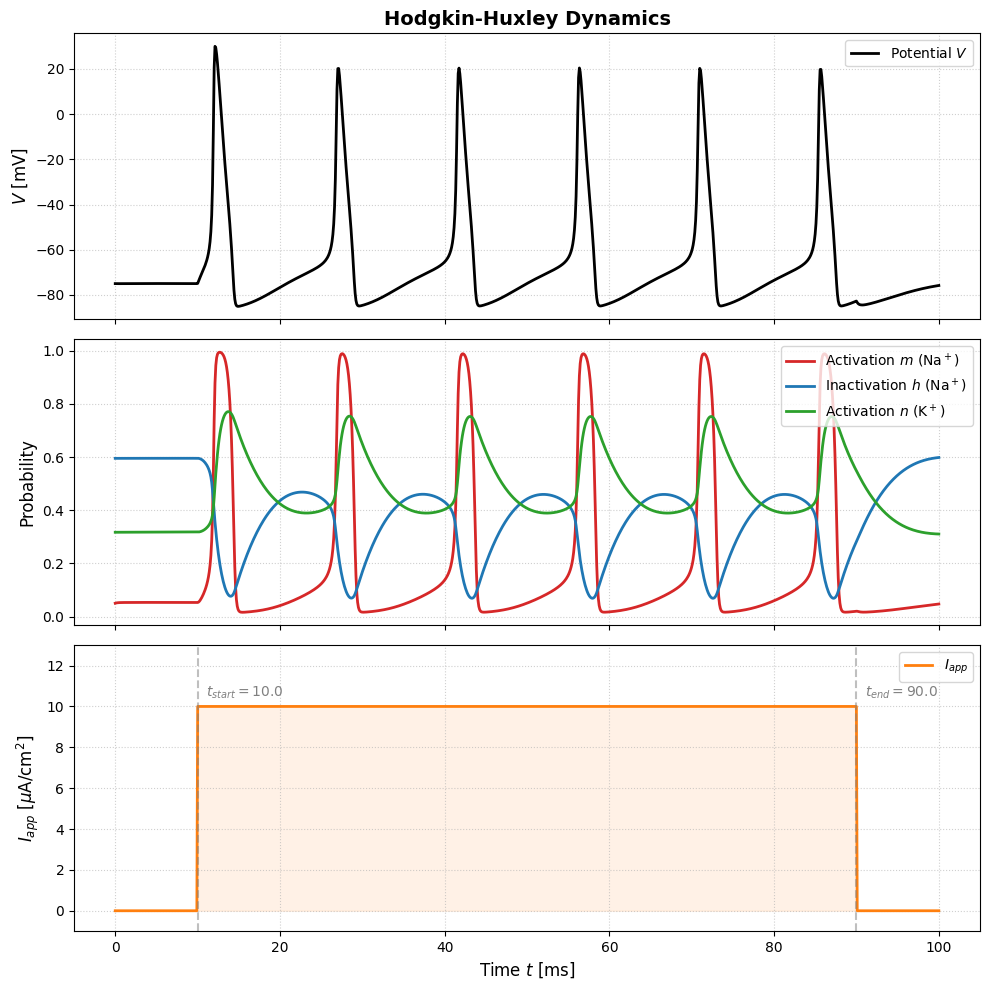
\includegraphics[width=\textwidth]{img/FH_model/HH_dynamics.png}
    \caption{Simulated dynamics of the Hodgkin-Huxley model. The plots illustrate the temporal evolution of the transmembrane potential $V$ along with the gating variables $m, h$, and $n$ under the influence of an applied external current $I_{app}(t)$.}
    \label{fig:hh_dynamics}
\end{figure}

\newpage
\section{The FitzHugh-Nagumo model}
The FitzHugh-Nagumo (FH) model \cite{centofanti2024comconf} is a two-dimensional simplification of the HH model that preserves the essential characteristics of excitability. The dynamical equations for the fast variable $V$ (potential) and the slow variable $w$ (recovery) are:

\begin{equation}
    \begin{aligned}
        \frac{dV}{dt} &= bV(V-\beta)(\delta-V) - cw + I_{app} \\
        \frac{dw}{dt} &= \epsilon(V - \gamma w)
    \end{aligned}
    \label{eq:FHN}
\end{equation}

The parameters used in all the FH simulations throughout this thesis are $b = 5$, $c = 1$, $\beta = 0.1$, $\delta = 1$, $\epsilon = 0.1$, $\gamma = 0.25$ \cite{centofanti2024comconf}.

\subsection*{Asymptotic behavior}
\label{sec:FHN_dynamics}
The dynamics of the FHN system depends on the value of $I_{app}$, which vertically translates the cubic nullcline, modifying the position and stability of the fixed point:

\begin{itemize}
    \item \textbf{Stable equilibrium regime ($I_{app} \lesssim 0.2$):} 
    The system presents a unique stable fixed point located on the left branch of the cubic nullcline (near the resting state). For small stimuli, the system returns to equilibrium without generating oscillations.
    
    \item \textbf{Oscillatory regime ($0.2 \lesssim I_{app} \lesssim 2.1$):} 
    When the current exceeds the first critical threshold ($I_{th1} \approx 0.21$), the fixed point enters the unstable region of the nullcline (between the two knees of the cubic). The equilibrium loses stability and a stable limit cycle emerges. The system produces sustained periodic oscillations, as highlighted in Figure \ref{fig:fhn_time_series} - \ref{fig:fhn_phase_space}.
    
    \item \textbf{Saturation regime ($I_{app} \gtrsim 2.1$):} 
    Increasing the current beyond the second critical threshold ($I_{th2} \approx 2.1$), the intersection of the nullclines shifts to the stable right branch. The limit cycle vanishes, and the system stabilizes at a high-potential equilibrium (permanent excited state).
\end{itemize}

\begin{figure}[H]
    \centering
    \begin{minipage}[b]{0.58\textwidth}
        \centering
        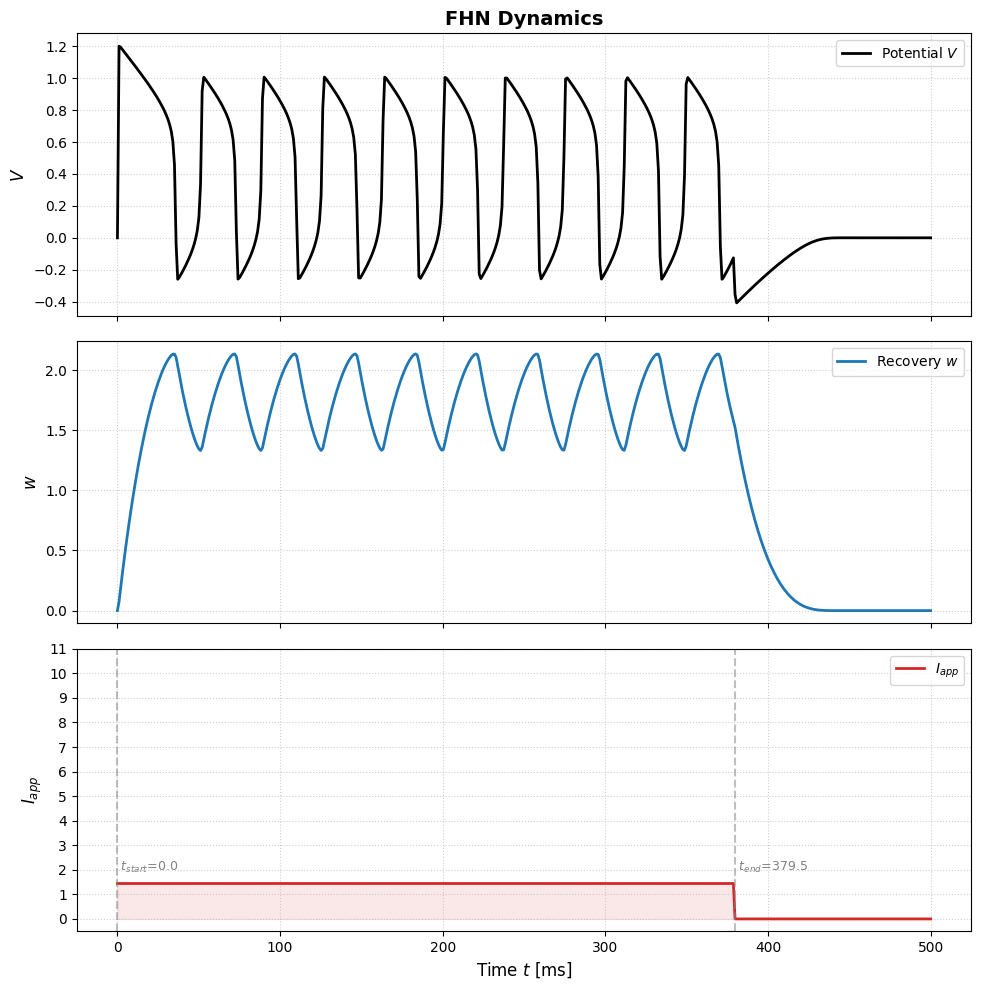
\includegraphics[width=\textwidth]{img/FH_model/No_Network/limit_cycle.png}
        \caption{Time evolution of $V$ and $w$ in the oscillatory regime.}
        \label{fig:fhn_time_series}
    \end{minipage}
    \hfill
    \begin{minipage}[b]{0.38\textwidth}
        \centering
        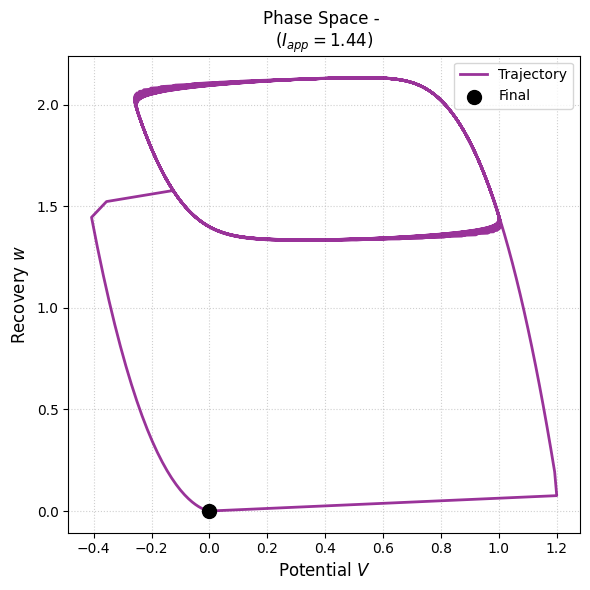
\includegraphics[width=\textwidth]{img/FH_model/No_Network/limit_cycle_phase_space.png}
        \caption{Trajectory in the phase plane $(V, w)$.}
        \label{fig:fhn_phase_space}
    \end{minipage}
    \caption*{Dynamics of the FitzHugh-Nagumo model with $I_{app} \approx 1.44$ (left: space-time, right: phase space). After a transient the system exhibits a stable limit cycle. Note that since the perturbation (bottom left) is a square wave once it goes off the system returns to the only stable equilibrium $(0,0)$.}
    \label{fig:fhn_dynamics}
\end{figure}


In Fig \ref{fig:fhn_time_series} we can see a response of the system to a square wave perturbation. In particular, we observe an oscillatory dynamics while the external current is on.
Since our ML analysis (chapter \ref{Chpt3}) is based on mapping  functions (perturbations) to functions (responses), we considered the square wave perturbation class as it provides an easy-to-study function basis

Starting from these premises, we turned to study the spatial extension of the FH model and analyzed its response to a square wave perturbation localized in space (i.e. applied to a single node).


\newpage
\section{From single neuron to spatially extended systems}
\label{sec:extended_network}
The framework discussed thus far has focused on the dynamics of an isolated single node. In order to transition from a microscopic to a mesoscopic description of neural dynamics, we embedded the FitzHugh-Nagumo (FHN) model within a network topology. Our primary objective was to investigate whether the resulting high-dimensional system of ordinary differential equations (ODEs) could be effectively approximated by a single neural operator trained via deep learning techniques, which will be detailed in Chapter \ref{Chp:2}.

To this end, we considered a spatially extended system characterized by a specific input-output mapping. An external stimulus, modeled as a square-wave current, was injected into a designated \textcolor{blue}{\textbf{input node}}. The signal then propagated through the network via diffusive coupling, while each node underwent local reaction dynamics governed by the FHN equations. Finally, the response of the system was recorded by extracting the membrane potential of a designated \textcolor{red}{\textbf{output node}}. This setup is illustrated by two examples in Figure \ref{fig:fh_comparison}.


Formally, let $\mathcal{G} = (\mathcal{V}, \mathcal{E})$ be an unweighted graph representing the neural network topology. The diffusive coupling between neurons are modeled using the elements $L_{ij}$ of the graph Laplacian matrix $\mathbf{L} = \mathbf{D}_{deg} - \mathbf{A}$, where $\mathbf{D}_{deg}$ is the diagonal degree matrix and $\mathbf{A}$ is the adjacency matrix. The elements of the Laplacian are explicitly defined as:
\begin{equation}
L_{ij} = 
\begin{cases} 
\text{deg}(i) & \text{if } i = j \\
-1 & \text{if } (i,j) \in \mathcal{E} \\
0 & \text{otherwise}
\end{cases}
\end{equation}

The dynamics of the coupled system are therefore governed by the following set of equations for each node $i \in \mathcal{V}$:
\begin{equation}
\label{eq:coupled_FHN}
\begin{aligned}
\frac{dV_i}{dt} &= b V_i (V_i - \beta)(\delta - V_i) - c w_i + I_{app, i}(t) - \sigma \sum_{j=1}^{|\mathcal{V}|} L_{ij} V_j \\
\frac{dw_i}{dt} &= \epsilon (V_i - \gamma w_i)
\end{aligned}
\end{equation}
where the coefficient $\sigma$ modulates the global coupling strength (i.e., the intensity of diffusion) across the network.
\begin{figure}[htbp]
    \centering
    % --- Prima immagine (sopra) ---
    \begin{subfigure}[b]{1.0\textwidth}
        \centering
        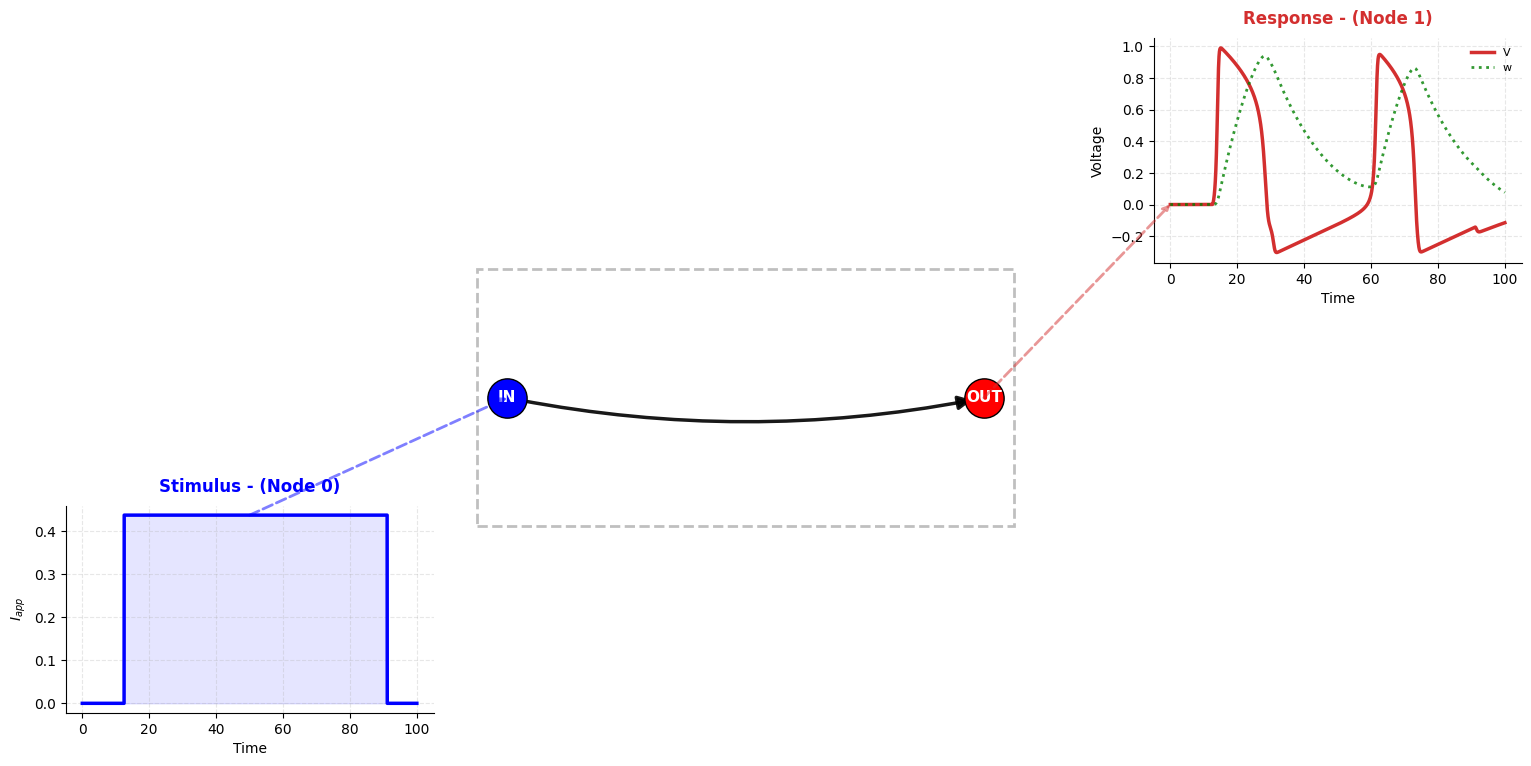
\includegraphics[width=\textwidth]{img/FH_model/1to2/output0to1_v2.png}
        \caption{Minimal setup: Input $\rightarrow$ Output}
        \label{fig:fh_output}
    \end{subfigure}
    
    \vspace{0.5cm} % Spazio verticale tra le due figure
    
    % --- Seconda immagine (sotto) ---
    \begin{subfigure}[b]{1.0\textwidth}
        \centering
        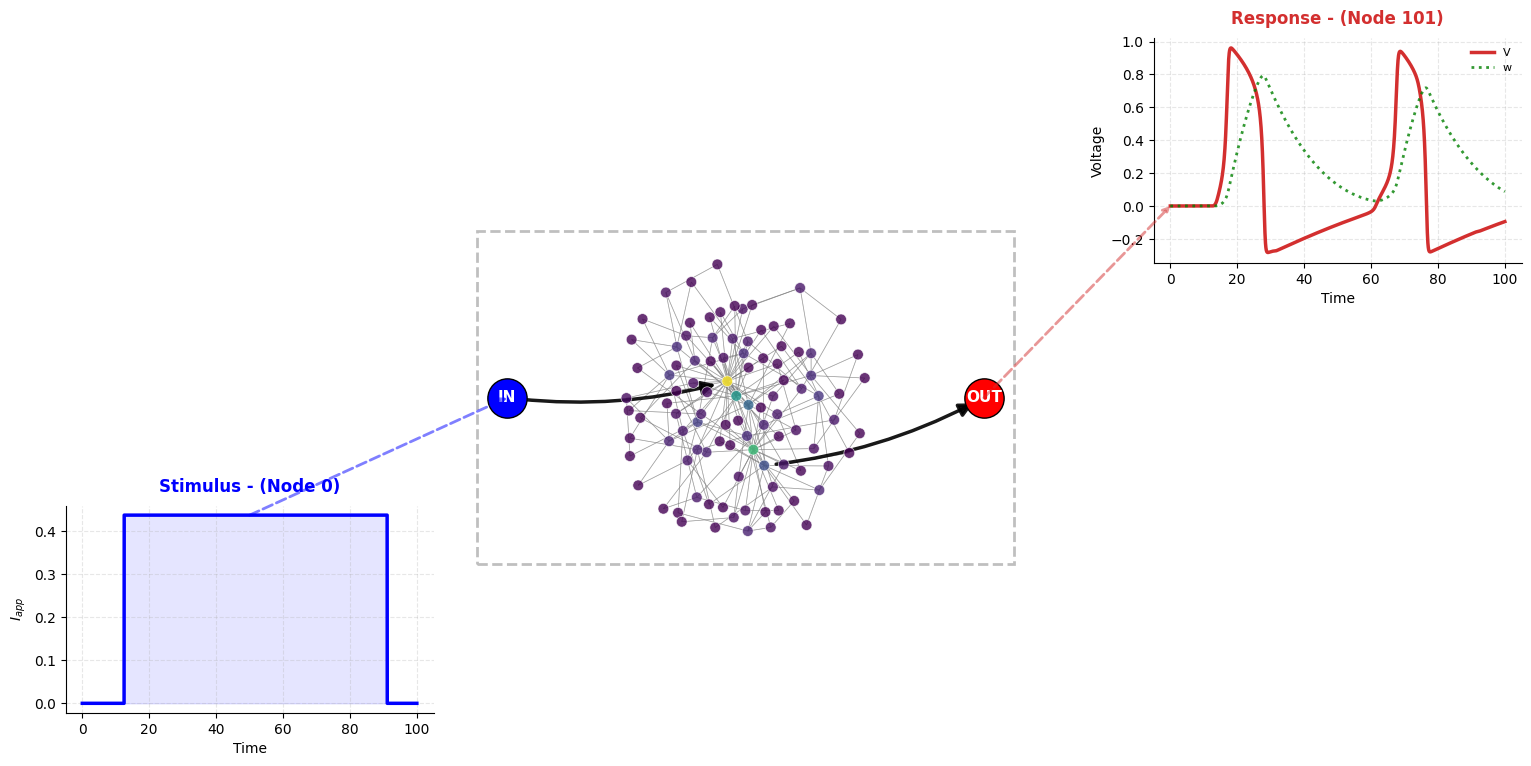
\includegraphics[width=\textwidth]{img/FH_model/BA_Network/network_plot_BA_N=100_v2.png}
        \caption{Extended topology: Input $\rightarrow$ Network $\rightarrow$ Output}
        \label{fig:fh_dynamics}
    \end{subfigure}
    
    \caption{Schematic representation of the network setup. (a) A minimal configuration illustrating the direct signal transmission from an input to an output node. (b) A more complex topology utilizing a Barabási-Albert (BA) scale-free network ($N=100$, $m=2$), demonstrating how the input stimulus propagates through a mesoscopic structure before reaching the output node.}
    \label{fig:fh_comparison}
\end{figure}

Having established the mathematical formulation of the coupled system, in the next chapter we will introduce the principles of Scientific Machine Learning (SciML). Specifically, we will focus on the operator learning techniques employed to emulate the input-output mapping of the spatially extended system—that is, predicting the continuous temporal evolution of the \textcolor{red}{\textbf{output node}}'s potential as a direct consequence of a specific perturbation applied to the \textcolor{blue}{\textbf{input node}}.

    \chapter{Chapter 2}
\label{Chp:2}
\section{A brief introduction to Machine Learning}
Machine Learning (ML) encompasses a broad set of methods that enable algorithms to learn complex patterns and relationships from data. While traditional approaches rely on manually engineering features, ML techniques automatically adjust their internal parameters to improve performance on a specific task. Here we specifically focus here on the application of Deep Learning, characterized by the utilization of Artificial Neural Networks (ANNs).

\begin{figure}[htbp]
    \centering
    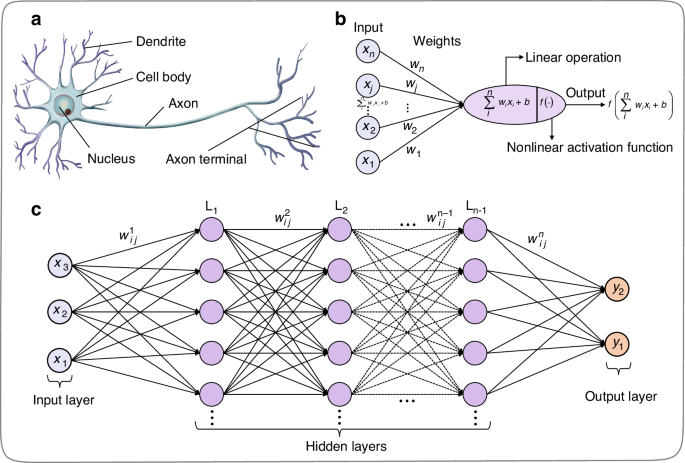
\includegraphics[width=0.95\textwidth]{img/ANN.png}
    \caption{Visual overview of neural networks. Panel a: A detailed illustration of a biological neuron with key structural components. Panel b: A schematic of an artificial neuron (Perceptron), demonstrating how weighted inputs are combined linearly and then passed through a non-linear activation function. Panel c: A Deep Neural Network, composed of stacked layers of artificial neurons, showing input, hidden, and output layers.}
    \label{fig:ann_overview}
\end{figure}

ANNs are computational models inspired by the structure and function of biological neural systems, which communicate via vast networks of neurons (fig.~\ref{fig:ann_overview}a). The fundamental computational unit is the artificial neuron (Fig.~\ref{fig:ann_overview}b). A single neuron computes a linear combination of its inputs $\mathbf{x}$ using a set of learnable weights $\mathbf{w}$ and a bias term $b$. This sum is then transformed by a non-linear activation function, $f(\cdot)$, which is essential for capturing complex, non-linear mappings.

By stacking these fundamental units into multiple layered structures, we create Deep Neural Networks (DNNs) (Fig.~\ref{fig:ann_overview}c). These architectures have proven highly effective in mapping high-dimensional function spaces and solving problems in diverse fields like computer vision, natural language processing, and physical modeling. A key theoretical foundation of ANNs is the \textit{Universal Approximation Theorem}. This theorem states that a feedforward network with a single hidden layer and a non-linear activation function can, in principle, approximate any continuous function on a compact set, given a sufficient number of neurons. First proven by Cybenko~\cite{cybenko1989approximation} and Hornik~\cite{hornik1989multilayer} in 1989, this principle highlights the fundamental expressive power of neural network architectures. Modern deep networks extend this concept by composing multiple non-linear transformations across numerous layers.


\section{Operator Learning}

Scientific Machine Learning (SciML) has emerged as a rapidly developing field that bridges the versatility of data-driven techniques—designed 
to recognize complex patterns from observations—with the rigor of traditional modeling based on partial differential equations (PDEs).

According to recent categorizations \cite{boulle2023mathematical}, the SciML landscape can be broadly divided into three main areas:
\begin{enumerate}
    \item \textbf{PDE Discovery}, which focuses on inverse problems to uncover governing equations from data;
    \item \textbf{Neural PDE Solvers}, which leverage neural networks to approximate the solution of specific PDE instances;
    \item \textbf{Operator Learning}, the most recent development, aimed at learning mappings between infinite-dimensional function spaces.
\end{enumerate}

The second area is related to direct problems and has proven effective in accelerating traditional solvers.
A revolution in this field was marked by the introduction of Physics-Informed Neural Networks (PINNs) and their variants \cite{raissi2019physics}. 
These architectures privilege a physics-oriented approach, embedding physical laws directly into the optimization process, rather than relying solely on data.
However, PINNs are typically trained to solve a \textit{single} problem instance efficiently. Since the solution depends on specific input parameters
or boundary conditions, changing these inputs often requires retraining the network, limiting their applicability in many-query scenarios.

To address this limitation, the third branch—\textbf{Operator Learning}—has been developed over the last few years \cite{lu2021learning, li2020fourier}.
 Unlike traditional solvers, operator learning algorithms aim to approximate the underlying operator itself, 
 mapping an entire class of input functions to their corresponding solutions. This approach has been successfully applied to complex PDE systems 
 involving parametric dependencies and forcing terms, as well as in industrial applications \cite{osorio2022forecasting}.

Among the emerging approaches, two architectures stand out: the Deep Operator Network (DeepONet) \cite{lu2021learning}, 
based on the universal approximation theorem for operators, and Neural Operators \cite{kovachki2023neural}. Specifically, 
integral kernel-based methods such as the Fourier Neural Operator (FNO) \cite{li2020fourier}
have demonstrated remarkable capabilities in learning non-linear operators on regular or equispaced domains.

\begin{figure}[htbp]
    \centering
    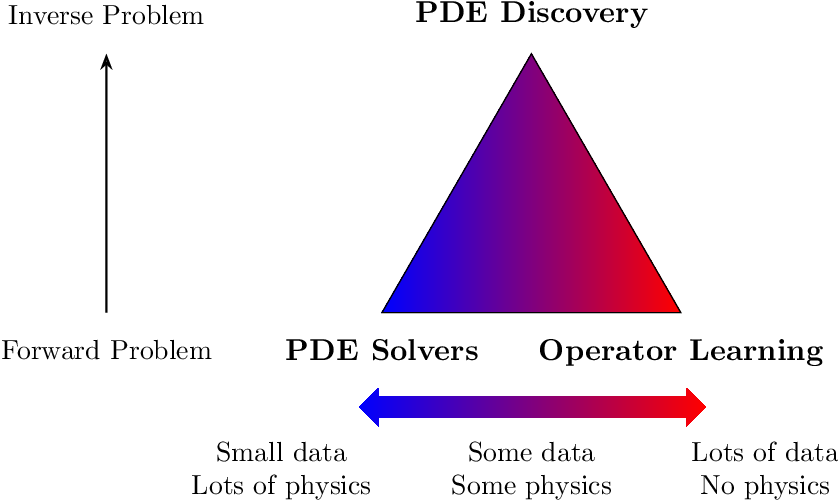
\includegraphics[width=0.75\textwidth]{img/Operator_learning.png}
    \caption{Visual representation of the Scientific Machine Learning (SciML) landscape.}
    \label{fig:sciml_landscape}
\end{figure}

\newpage

\subsection{Neural Architectures}
\subsubsection{Deep Operator Network (DeepONet)}
The DeepONet, introduced by Lu et al. \cite{lu2021learning}, was the first architecture explicitly designed as a concrete realization of the universal approximation theorem for operators by Chen and Chen \cite{Chen_Chen_1995}.
The architecture, schematized in Figure \ref{fig:deeponet_schema}, is composed of two distinct neural subnetworks working in parallel:
\begin{itemize}
    \item \textbf{Branch Network:} encodes the input function $f$ evaluated at a finite number of sensor points $x_1, \dots, x_m$.
    \item \textbf{Trunk Network:} encodes the domain coordinates $y$ where the solution is to be evaluated.
\end{itemize}
The output of the approximated operator is obtained through the dot product of the outputs of these two networks, allowing the solution to generalize across the entire continuous domain \cite{lu2021learning}:
\begin{equation}
    \hat{G}_{\theta}(f)(y) = \sum_{k=1}^{p} \underbrace{b_k(f(x_1), \dots, f(x_m))}_{\text{Branch Net}} \cdot \underbrace{t_k(y)}_{\text{Trunk Net}}
\end{equation}

\begin{figure}[H]
    \centering
    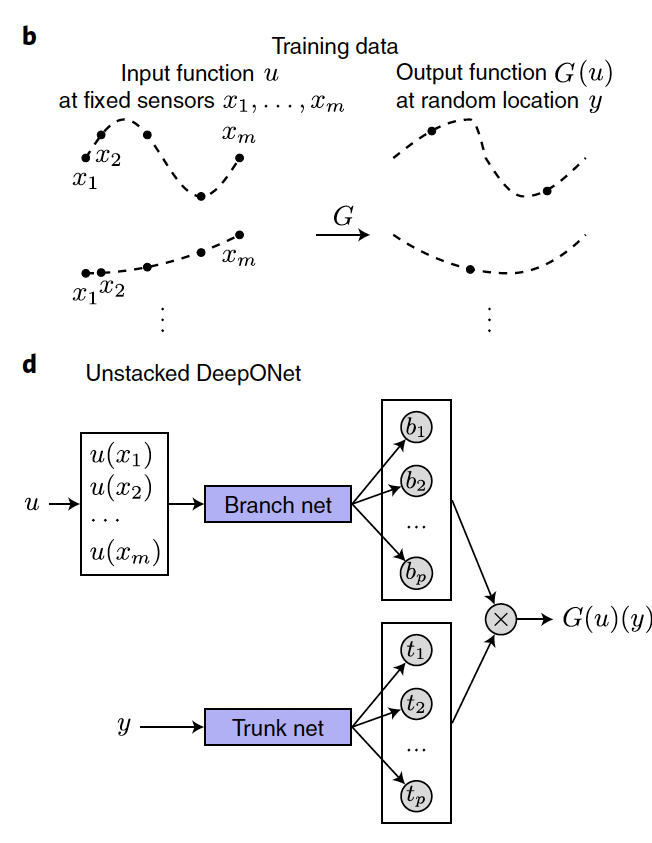
\includegraphics[width=0.8\textwidth]{img/FH_model/DeepONet.png}
    \caption{Schematic of the DeepONet architecture. The \textit{branch net} processes the discretized input function, while the \textit{trunk net} processes the domain coordinates. Their outputs are combined via a dot product. Adapted from \cite{lu2021learning}.}
    \label{fig:deeponet_schema}
\end{figure}

\subsubsection{Fourier Neural Operator (FNO)}
The Fourier Neural Operator (FNO), proposed by Li et al. \cite{li2020fourier}, tackles the approximation problem by parameterizing the integral operator directly in the frequency domain. Unlike standard networks, FNO learns a mapping between infinite-dimensional function spaces, guaranteeing discretization independence (\textit{resolution-invariance}).

As shown in Figure \ref{fig:fno_schema}, the architecture follows three main phases:
\begin{enumerate}
    \item \textbf{Lifting:} The input $a(x)$ is lifted to a higher-dimensional hidden representation $v_0(x)$ via a local transformation $P$ (typically a shallow fully connected network with activation $\sigma_1$): \\
    $v_0(x) = P(a(x)) = \sigma_1(W_{\text{in}} a(x) + b_{\text{in}}), \quad x \in D.$
    
    \item \textbf{Iterative Kernel Updates:} For $t = 0, \dots, T-1$, the hidden representation is updated using a pointwise linear operator $W_t$, an integral kernel operator with parameterized kernel $\kappa_t$, and the non-linear activation function $\sigma_2$: \\
    $\displaystyle v_{t+1}(x) = \sigma_2 \left( W_t v_t(x) + \int_{D} \kappa_t(x,y) v_t(y) \, dy + b_t \right).$
    
    \item \textbf{Projection:} The final hidden representation $v_T$ is projected back to the target space defined on $D'$ using another local transformation $Q$ (with activation $\sigma_3$): \\
    $\mathcal{G}(a)(x) = Q(v_T(x)) = \sigma_3(W_{\text{out}} v_T(x) + b_{\text{out}}), \quad x \in D'.$
\end{enumerate}

In the specific case of the Fourier Neural Operator (FNO) \cite{li2020fourier}, the integral kernel is parameterized directly in the frequency domain. By leveraging the convolution theorem, the continuous integral operation is efficiently resolved by computing the Fourier transform of the input, performing a pointwise multiplication with a learnable complex-valued weight tensor over a truncated set of low-frequency modes,
%Devo parlare della relazione che deve intercorrere tra le frequenze considerate $k_max$ ed il numero di campioni $N$ (Teorema di Nysquist-Shannon?)
 and finally applying the inverse Fourier transform. Mathematically, the integral term in the iterative update is replaced by:
\[ 
\int_{D} \kappa_t(x,y) v_t(y) \, dy = \mathcal{F}^{-1} \left( R_t \cdot \mathcal{F}(v_t) \right)(x) 
\]
where $\mathcal{F}$ and $\mathcal{F}^{-1}$ denote the forward and inverse Fourier transforms, respectively, and $R_t$ is the learnable complex tensor acting as the Fourier kernel at layer $t$. The truncation of higher frequencies acts as a low-pass filter, ensuring both discretization invariance and high computational efficiency.

\begin{figure}[H]
    \centering
    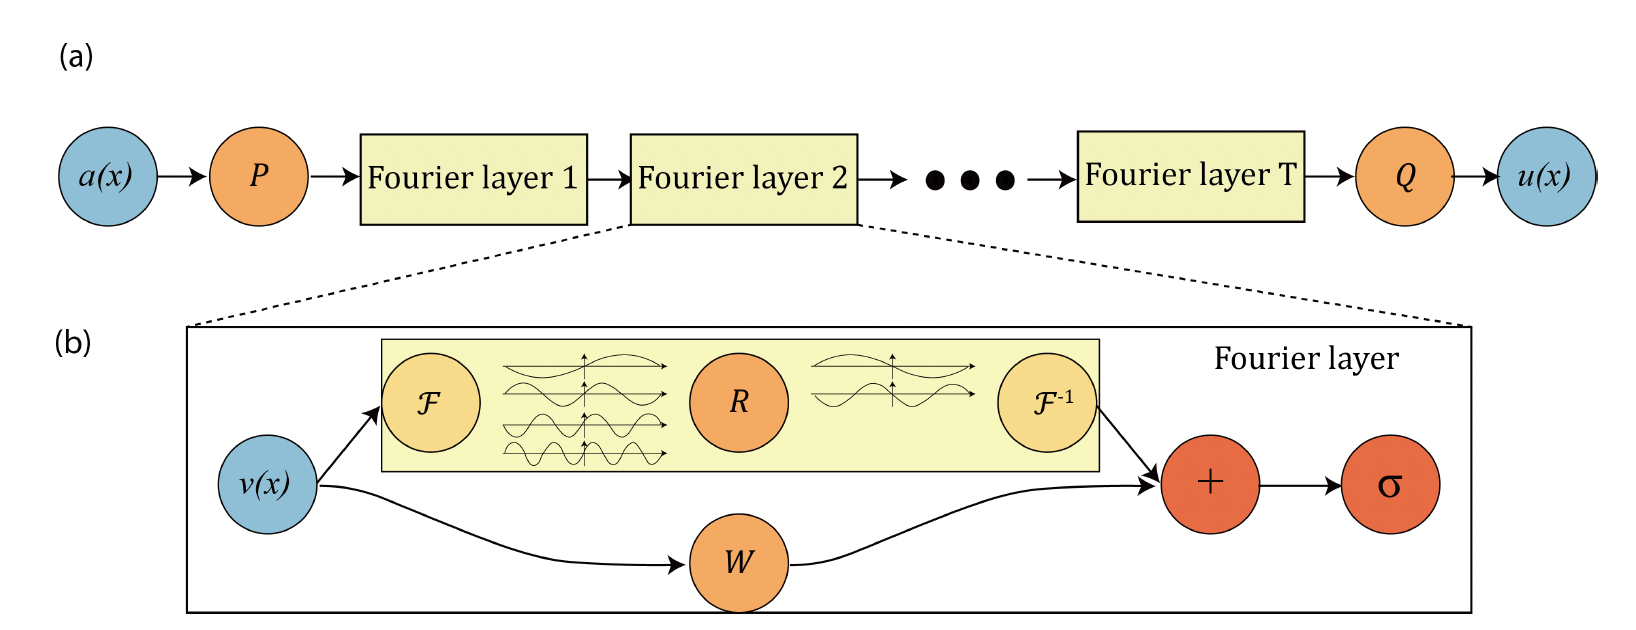
\includegraphics[width=\textwidth]{img/FH_model/FNO.png}
    \caption{Schematic of the FNO architecture. (a) General structure with lifting ($P$), iterative layers ($T$), and projection ($Q$). (b) Detail of a single Fourier layer. Adapted from \cite{li2020fourier}.}
    \label{fig:fno_schema}
\end{figure}

\newpage
\section{Approximation theorems}
\subsection{Universal approximation of functions}
To fully understand the universal approximation capabilities of Artificial Neural Networks, we first need to introduce the formal mathematical framework and notation established by Hornik, Stinchcombe, and White \cite{hornik1989multilayer}. 

Let $r \in \mathbb{N}$ be the dimension of the input space. We define $A^r$ as the set of all affine functions mapping $\mathbb{R}^r$ to $\mathbb{R}$:
$$ A^r = \{ A: \mathbb{R}^r \to \mathbb{R} \mid A(x) = w \cdot x + b, \; w, x \in \mathbb{R}^r, \; b \in \mathbb{R} \} $$
In a neural network context, $x$ represents the network input, $w$ the weights from the input to the intermediate layer, and $b$ the bias term.

A fundamental component of these architectures is the activation function, specifically a \textbf{squashing function}. A function $\Psi: \mathbb{R} \to [0, 1]$ is defined as a squashing function if it is \textit{non-decreasing}, $ \mathit{\lim_{\lambda \to \infty} \Psi(\lambda) = 1}$, and $\mathit{\lim_{\lambda \to -\infty} \Psi(\lambda) = 0}$.

Using these components, we define the class of output functions for a single hidden layer feedforward network. For any squashing function $\Psi$, the set $\Sigma^r(\Psi)$ is defined as:
$$ \Sigma^r(\Psi) = \left\{ f: \mathbb{R}^r \to \mathbb{R} \mathrel{\Big|} f(x) = \sum_{j=1}^q \beta_j \Psi(A_j(x)), \; \beta_j \in \mathbb{R}, \; A_j \in A^r, \; q \in \mathbb{N} \right\} $$
This represents the familiar class of output functions for networks with squashing at the hidden layer and a linear output layer, where the scalars $\beta_j$ correspond to the weights from the hidden to the output layer.

To rigorously evaluate how well these networks approximate other functions, we introduce the relevant mathematical spaces defined over the domain $\mathbb{R}^r$:
\begin{itemize}
    \item $\mathcal{B}^r$: The Borel $\sigma$-algebra on $\mathbb{R}^r$.
    \item $M^r$: The set of all Borel measurable functions $f: \mathbb{R}^r \to \mathbb{R}$.
    \item $C^r$: The set of all continuous functions $f: \mathbb{R}^r \to \mathbb{R}$ (note that $C^r \subset M^r$).
\end{itemize}

Finally, we define the approximation metrics:
\begin{itemize}
    \item \textbf{Uniformly dense on compacta:} A subset $S$ is uniformly dense on compacta in $C^r$ if, for every compact subset $K \subset \mathbb{R}^r$, $S$ is dense in $C^r$ with respect to the supremum metric $\rho_K(f, g) = \sup_{x \in K} |f(x) - g(x)|$.
    \item \textbf{$\rho_\mu$-dense:} Given a probability measure $\mu$ on $(\mathbb{R}^r, \mathcal{B}^r)$, which describes the relative frequency of occurrence of input patterns, we define the metric $\rho_\mu(f, g) = \inf\{\epsilon > 0 : \mu\{|f(x) - g(x)| > \epsilon\} < \epsilon\}$. Two functions are close in this metric if they differ significantly only on a set of inputs with a vanishingly small probability.
\end{itemize}

With this framework, we can state the fundamental approximation theorem for standard ANNs:

\begin{theorem}[Hornik, Stinchcombe, White, 1989]
For every squashing function $\Psi$, every $r$, and every probability measure $\mu$ on $(\mathbb{R}^r, \mathcal{B}^r)$, $\Sigma^r(\Psi)$ is uniformly dense on compacta in $C^r$ and $\rho_\mu$-dense in $M^r$.
\end{theorem}

%Il teorema generale è per più layers (almeno uno hidden). Lascio questa versione?

\subsection{Universal approximation of operators}

The universal approximation theorem by Hornik et al. guarantees that standard neural networks can approximate any continuous function between finite-dimensional spaces. However, many physical systems and partial differential equations (PDEs) require mapping an infinite-dimensional space to another infinite-dimensional space (e.g., mapping a parametric initialization or a boundary condition to a complete solution field over time). To address this, the operator learning paradigm extends the concept of universal approximation to operators.

The foundational theoretical work for operator approximation was established by Chen and Chen \cite{Chen_Chen_1995}, who demonstrated that a neural network with a specific architecture can approximate any continuous nonlinear operator. This theorem directly inspired the DeepONet architecture \cite{lu2021learning}.

Let $K_1 \subset \mathbb{R}^{d_1}$ and $K_2 \subset \mathbb{R}^{d_2}$ be compact sets. Let $V$ be a compact set in the space of continuous functions $C(K_1)$. We define a continuous nonlinear operator $\mathcal{G} : V \to C(K_2)$. 

\begin{theorem}[Universal Approximation Theorem for Operators, Chen \& Chen, 1995]
Suppose $\sigma$ is a continuous non-polynomial function. For any $\epsilon > 0$, there exist positive integers $n, m$, points $x_1, \dots, x_m \in K_1$, and constants $c_i, \xi_{ij}, \theta_i, \zeta_i \in \mathbb{R}$, $w_i \in \mathbb{R}^{d_2}$ (for $i=1,\dots,n$ and $j=1,\dots,m$) such that:
$$ \left| \mathcal{G}(u)(y) - \sum_{i=1}^n c_i \sigma \left( \sum_{j=1}^m \xi_{ij} u(x_j) + \theta_i \right) \sigma(w_i \cdot y + \zeta_i) \right| < \epsilon $$
holds for all $u \in V$ and $y \in K_2$.
\end{theorem}

This theorem explicitly reflects the dual-network structure of DeepONet. The term $\sigma\left(\sum_{j=1}^m \xi_{ij} u(x_j) + \theta_i\right)$ is parameterized by the \textit{branch net}, which takes discrete evaluations of the input function $u$ at sensor locations $x_j$. Conversely, the term $\sigma(w_i \cdot y + \zeta_i)$ is parameterized by the \textit{trunk net}, which evaluates the continuous spatial or temporal coordinates $y$.


\subsection{Universal approximation of operators II}

While the theorem by Chen and Chen \cite{Chen_Chen_1995} provides a fundamental result for continuous functions on compact sets, modern Scientific Machine Learning tasks often require learning operators under specific physical constraints, working with Lebesgue or Sobolev spaces, and minimizing the expected error over a specific probability measure of the initial conditions or parameters.

Kovachki et al. \cite{kovachki2023neural} provide a comprehensive approximation theory for Neural Operators, proving that an architecture based on alternating integral kernel operators and pointwise non-linearities is a universal approximator for operators between general Banach spaces. 

To formally state the theorems, we first need to define the function spaces for which these results hold.

\subsection{Function Space Assumptions}

The theory relies on the input and output spaces possessing the \textit{Banach Space Approximation Property (AP)}, which allows infinite-dimensional operators to be approximated by finite-rank operators. The authors restrict the analysis to the following widely used spaces.

\begin{assumption}[Input Space $\mathcal{A}$]
Let $D \subset \mathbb{R}^d$ be a Lipschitz domain. The input Banach space $\mathcal{A}$ satisfies one of the following:
\begin{enumerate}
    \item $\mathcal{A} = L^{p_1}(D)$ for some $1 \le p_1 < \infty$;
    \item $\mathcal{A} = W^{m_1,p_1}(D)$ for some $1 \le p_1 < \infty$ and $m_1 \in \mathbb{N}$;
    \item $\mathcal{A} = C(\overline{D})$.
\end{enumerate}
\end{assumption}

\begin{assumption}[Output Space $\mathcal{U}$]
Let $D' \subset \mathbb{R}^{d'}$ be a Lipschitz domain. The output Banach space $\mathcal{U}$ satisfies one of the following:
\begin{enumerate}
    \item $\mathcal{U} = L^{p_2}(D')$ for some $1 \le p_2 < \infty$ and $m_2 = 0$;
    \item $\mathcal{U} = W^{m_2,p_2}(D')$ for some $1 \le p_2 < \infty$ and $m_2 \in \mathbb{N}$;
    \item $\mathcal{U} = C^{m_2}(\overline{D}')$ with $m_2 \in \mathbb{N}_0$.
\end{enumerate}
\end{assumption}

The theoretical architecture of the Neural Operator, denoted as $NO_N(\sigma_1, \sigma_2, \sigma_3; D, D')$, represents the class of neural operators where $N \in \mathbb{N}$ is the number of integral layers (the depth of the network), $\sigma_1, \sigma_2, \sigma_3$ are the non-linear activation functions used respectively for the initial lifting mapping, the iterative kernel layers, and the final projection mapping, while $D$ and $D'$ are the input and output spatial domains. This architecture is specifically constructed so that its continuous layers can seamlessly approximate infinite-dimensional mappings with arbitrary precision. Note that for FNO $D=D'$.

\begin{theorem}[Uniform Universal Approximation, Kovachki et al. \cite{kovachki2023neural}]
Suppose the spaces $\mathcal{A}$ and $\mathcal{U}$ satisfy the aforementioned Assumptions and let $\mathcal{G}^{\dagger} : \mathcal{A} \to \mathcal{U}$ be a continuous operator. Let $\sigma_1, \sigma_2, \sigma_3$ be suitable non-polynomial continuous activation functions. 
Then, for any compact set $K \subset \mathcal{A}$ and any $\epsilon > 0$, there exists an integer $N \in \mathbb{N}$ and a Neural Operator $\mathcal{G} \in NO_N(\sigma_1, \sigma_2, \sigma_3; D, D')$ such that:
\[ 
\sup_{a \in K} \left\| \mathcal{G}^{\dagger}(a) - \mathcal{G}(a) \right\|_{\mathcal{U}} \le \epsilon 
\]
Furthermore, if $\mathcal{U}$ is a Hilbert space and there exists $M > 0$ such that $\|\mathcal{G}^{\dagger}(a)\|_{\mathcal{U}} \le M$ for all $a \in \mathcal{A}$, then $\mathcal{G}$ can be chosen such that uniformly $\|\mathcal{G}(a)\|_{\mathcal{U}} \le 4M$ for all $a \in \mathcal{A}$.
\end{theorem}

\newpage
\section{Discretization invariance and resolution independence}

A defining characteristic of Neural Operators, which distinguishes them from classical deep learning architectures such as Convolutional Neural Networks (CNNs), is the property of \textit{discretization invariance}. In standard architectures, model parameters are intrinsically tied to the specific discretization of the input data (e.g., the number of pixels in an image or the grid size of a simulation). Conversely, Neural Operators are defined as mappings between infinite-dimensional function spaces, meaning the learned parameters are independent of the underlying mesh used during training \cite{kovachki2023neural}.

\subsection{Intuition}

An operator learning architecture is said to be discretization-invariant if the model parameters $\theta$ are defined in a continuous function space and can be applied to any discretization of the input and output domains $D, D'$. 

Following Li et al. \cite{li2020fourier}, let $a \in \mathcal{A}$ be the input function. In a practical setting, we only observe $a$ at a finite set of points $\{x_1, \dots, x_n\} \subset D$. While a standard neural network would learn a mapping $\mathbb{R}^n \to \mathbb{R}^m$, the Neural Operator learns an operator $\mathcal{G}_{\theta}: \mathcal{A} \to \mathcal{U}$. The discretization $a_n$ of the function $a$ is used only to approximate the continuous integral:
\[ 
\int_{D} \kappa(x,y) v(y) \, dy \approx \sum_{j=1}^{n} \kappa(x, y_j) v(y_j) \Delta y_j 
\]
Because the kernel $\kappa$ (or its Fourier representation $R$ in FNOs) is a continuous object, the same parameters $\theta$ can be evaluated on a different set of points $\{x'_1, \dots, x'_k\}$ without retraining.

\subsection{Formal definition}

Since our data $a^{(i)}$ and $u^{(i)}$ are, in general, functions, to work with them numerically, we assume access only to their point-wise evaluations. To illustrate this, we will continue with the example of the preceding paragraph. For simplicity, assume $D = D'$ and suppose that the input and output functions are both real-valued. Let $D_L = \{x_{\ell}\}_{\ell=1}^L \subset D$ be an $L$-point discretization of the domain $D$ and assume we have observations $a^{(i)}|_{D_L}, u^{(i)}|_{D_L} \in \mathbb{R}^L$, for a finite collection of input-output pairs indexed by $i$. 

In the next section, we propose a kernel-inspired graph neural network architecture which, while trained on the discretized data, can produce the solution $u(x)$ for any $x \in D$ given an input $a \sim \mu$. In particular, our discretized architecture maps into the space $\mathcal{U}$ and not into a discretization thereof. Furthermore, our parametric operator class is consistent, in that, given a fixed set of parameters, refinement of the input discretization converges to the true function space operator. We make this notion precise in what follows and refer to architectures that possess it as \textit{function space architectures}, \textit{mesh-invariant architectures}, or \textit{discretization-invariant architectures}.

\begin{definition}[Discrete refinement]
We call a discrete refinement of the domain $D \subset \mathbb{R}^d$ any sequence of nested sets $D_1 \subset D_2 \subset \dots \subset D$ with $|D_L| = L$ for any $L \in \mathbb{N}$ such that, for any $\epsilon > 0$, there exists a number $L = L(\epsilon) \in \mathbb{N}$ such that
\[
D \subseteq \bigcup_{x \in D_L} \{y \in \mathbb{R}^d : \|y - x\|_2 < \epsilon\}.
\]
\end{definition}

\begin{definition}[Discretization]
Given a discrete refinement $(D_L)_{L=1}^{\infty}$ of the domain $D \subset \mathbb{R}^d$, any member $D_L$ is called a discretization of $D$.
\end{definition}

Since $a : D \subset \mathbb{R}^d \to \mathbb{R}^m$, pointwise evaluation of the function (discretization) at a set of $L$ points gives rise to the data set $\{(x_{\ell}, a(x_{\ell}))\}_{\ell=1}^L$. Note that this may be viewed as a vector in $\mathbb{R}^{L \times d} \times \mathbb{R}^{L \times m}$.

\begin{definition}[Discretized uniform risk]
Suppose $\mathcal{A}$ is a Banach space of $\mathbb{R}^m$-valued functions on the domain $D \subset \mathbb{R}^d$. Let $G : \mathcal{A} \to \mathcal{U}$ be an operator, $D_L$ be an $L$-point discretization of $D$, and $\hat{G} : \mathbb{R}^{L \times d} \times \mathbb{R}^{L \times m} \to \mathcal{U}$ some map. For any $K \subset \mathcal{A}$ compact, we define the discretized uniform risk as:
\[
R_K(G, \hat{G}, D_L) = \sup_{a \in K} \| \hat{G}(D_L, a|_{D_L}) - G(a) \|_{\mathcal{U}}.
\]
\end{definition}

\begin{definition}[Discretization-invariant]
Let $\Theta \subseteq \mathbb{R}^p$ be a finite dimensional parameter space and $G : \mathcal{A} \times \Theta \to \mathcal{U}$ a map representing a parametric class of operators with parameters $\theta \in \Theta$. Given a discrete refinement $(D_n)_{n=1}^{\infty}$ of the domain $D \subset \mathbb{R}^d$, we say $G$ is discretization-invariant if there exists a sequence of maps $\hat{G}_1, \hat{G}_2, \dots$ where $\hat{G}_L : \mathbb{R}^{L \times d} \times \mathbb{R}^{L \times m} \times \Theta \to \mathcal{U}$ such that, for any $\theta \in \Theta$ and any compact set $K \subset \mathcal{A}$,
\[
\lim_{L \to \infty} R_K(G(\cdot, \theta), \hat{G}_L(\cdot, \cdot, \theta), D_L) = 0.
\]
\end{definition}

Such a property is highly desirable as it allows a transfer of solutions between different grid geometries and discretization sizes with a single architecture that has a fixed number of parameters. From the construction of neural operators, when the input and output functions are evaluated on fixed grids, the architecture of neural operators on these fixed grids coincide with the class of neural networks.

\subsection{Zero-Shot Super-Resolution}

The immediate consequence of discretization invariance is the ability to perform \textit{zero-shot super-resolution}. The neural operator is mesh-invariant, so it can be trained on a lower resolution and evaluated at a
higher resolution, without seeing any higher resolution data. 

As demonstrated in the numerical experiments for parametric PDEs \cite{li2020fourier}, the error of a discretization-invariant model remains consistent across different resolutions. This is formally expressed by the property that as the discretization becomes finer ($n \to \infty$), the discrete approximation converges to the continuous operator:
\[ 
\lim_{n \to \infty} \mathcal{G}_{\theta}(a_n) = \mathcal{G}_{\theta}(a) 
\]
This feature is particularly valuable in neuroscience and complex systems modeling, where neural field dynamics or networked ODEs may be simulated at different spatial scales. A Neural Operator trained on a low-resolution brain atlas or a small neural network can, in principle, generalize its learned dynamics to higher-resolution representations or larger networks without requiring new training data.




    % --------------------------
    \part{\label{prt:First section}Emulation of a Neuronal System} % NOTE: dividing in parts is optional
    \chapter{Chapter 3}

\section{Problem definition}
\label{chpt: Problem definition}
In this work we expand on the results presented in \cite{centofanti2024comconf}, and developed in \cite{centofanti2024cma} and \cite{pellegrini2025mlcse}. In these articles an operator learning architecture (with a particular focus on FNO \footnote{see section ...}) has been used to learn the dynamics of a neuronal system, described by a ionic model (the FitzHugh-Nagumo or Hudgin-Huxely model \footnote{see section ...}). 
First of all the reaction has been simulated numerically by solving the underlying stiff systems of ordinary differential equations (ODEs). In the earlier works \cite{centofanti2024comconf, centofanti2024cma}, the MATLAB routine \texttt{ode15s} was utilized to integrate the equations over a fixed timespan (e.g., 100 ms) and the solutions were sampled on a uniform equispaced grid of 500 points. In the most recent development \cite{pellegrini2025mlcse}, which extends the study to higher-dimensional systems like the O'Hara-Rudy model, a Runge-Kutta method was employed. In all cases, the systems were perturbed using time-dependent applied currents, typically in the form of square pulses with varying intensities and durations, to explore the threshold-dependent dynamics and complex oscillatory behaviors of the cells.

The numerical solutions were then collected to construct the datasets for the operator learning task. Specifically, in the initial studies on the FitzHugh-Nagumo and Hodgkin-Huxley models, the authors generated a total of 2000 trajectories, split into 1600 samples for the training set and 400 for the test set \cite{centofanti2024comconf, centofanti2024cma}. Subsequently, to handle the increased complexity and ensure comprehensive coverage of the dynamical behaviors in higher-dimensional spaces, the dataset size was expanded to a total of 3750 trajectories, comprising 3000 training examples, 375 for validation, and 375 for testing \cite{pellegrini2025mlcse}.

Using these datasets, a Fourier Neural Operator (FNO) was trained to learn the non-linear mapping from the applied input current to the system's state variables (i.e., transmembrane potential, recovery, and gating variables). By leveraging the Fast Fourier Transform (FFT) on the uniform discretization grid, the FNO architecture computes the integral kernel operator directly in the frequency domain. This approach proved highly effective in capturing the global dependencies and multiscale temporal behaviors of the stiff ionic models, maintaining stable training and achieving very low relative $L^2$ errors across all the investigated dimensionalities.

The results across these studies demonstrate that FNOs are highly effective in learning the dynamics of stiff ionic models, consistently achieving low relative $L^2$ errors. Specifically, the optimized FNO architectures attained test errors of approximately 2.0\% for the FitzHugh-Nagumo model \cite{centofanti2024comconf}, 1.4\% for the Hodgkin-Huxley model \cite{centofanti2024cma}, and around 2.0\% even for the highly complex 41-variable O'Hara-Rudy model \cite{pellegrini2025mlcse}. Furthermore, the most recent findings emphasize the remarkable scalability of this approach: despite the substantial increase in system dimensionality, properly tuned FNOs maintain bounded training and test errors, with memory usage and training time scaling only linearly \cite{pellegrini2025mlcse}. This confirms the capability of FNOs to accurately and efficiently capture complex multiscale electrophysiological dynamics, gracefully overcoming the curse of dimensionality that typically affects artificial neural networks in high-dimensional settings.

% Versione senza "curse of dimensionality"
%This confirms the capability of FNOs to accurately and efficiently capture complex multiscale electrophysiological dynamics, exhibiting a linear scaling of memory and training time with respect to the system's dimensionality, while maintaining bounded parameters and relative errors \cite{pellegrini2025mlcse}.


\begin{figure}[htbp]
    \centering
    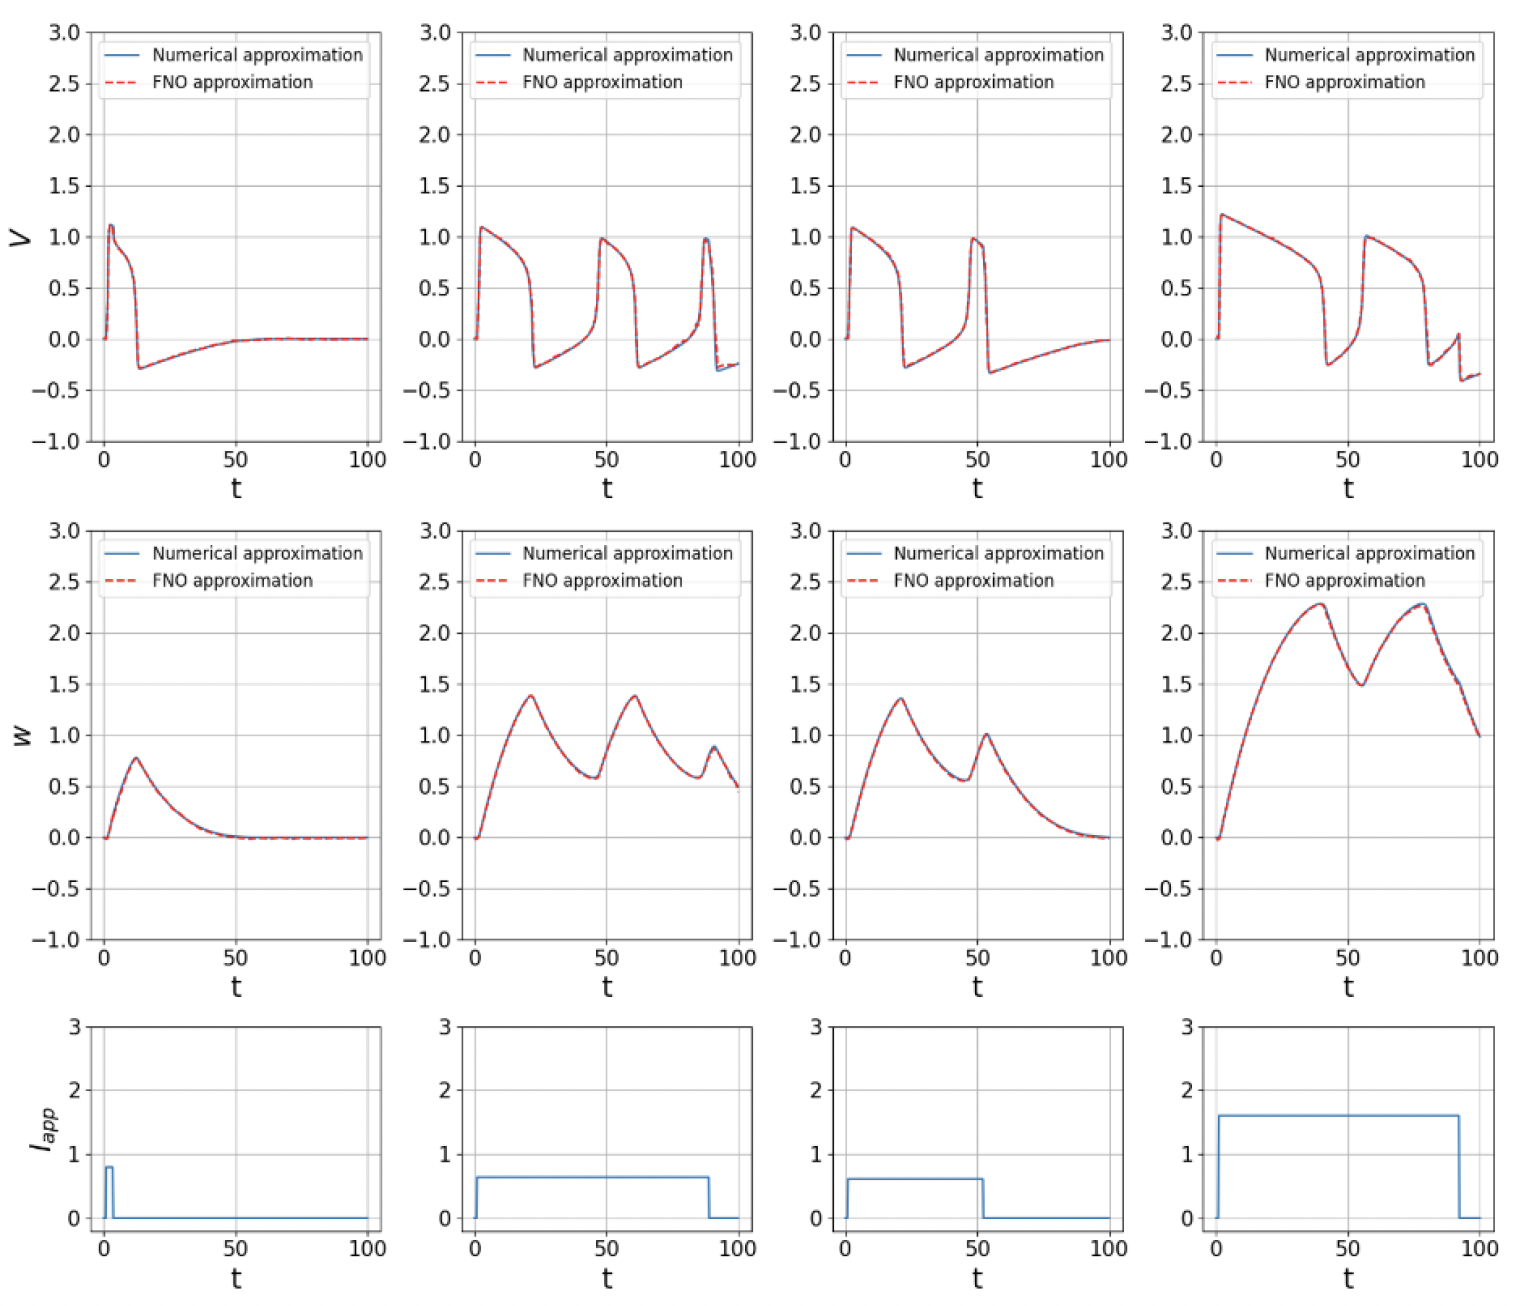
\includegraphics[width=0.55\textwidth]{img/FH_model/No_Network/Centofanti_article_figure.png}
    \caption{Numerical and FNO approximations in four tests (one per column): output potential $V$ (top), output recovery variable $w$ (center) and corresponding input current $I_{app}$ (bottom).}
    \label{fig:centofanti_dynamics}
\end{figure}

\newpage
\section{From single neuron to spatially extended systems}
However, the setup considered is that of a single node.
We generalized this approach by analyzing a spatial extended system: a current (in the form of square wave) is given as input to an \textcolor{blue}{\textbf{input node}}, information is transmitted through diffusion (where each node has a local reaction term following FitzHugh-Nagumo, see eq \eqref{eq:coupled_FHN}), and the potential is read/ predicted by the NN for the \textcolor{red}{\textbf{output node}}.


\begin{figure}[htbp]
    \centering
    % --- Prima immagine (sinistra) ---
    \begin{subfigure}[b]{0.48 \textwidth}
        \centering
        
\includegraphics[width=\textwidth]{img/FH_model/1to2/output0to1.png}
        \caption{Input $\rightarrow$ Output}
        \label{fig:fh_output}
    \end{subfigure}
    \hfill % <--- Questo inserisce uno spazio elastico tra le due immagini
    % --- Seconda immagine (destra) ---
    \begin{subfigure}[b]{0.48\textwidth}
        \centering
        
\includegraphics[width=\textwidth]{img/FH_model/Simple_cycle/dynamics_cycle.png}
        \caption{Input $\rightarrow$ Network $\rightarrow$ Output}
        \label{fig:fh_dynamics}
    \end{subfigure}
    
    % Didascalia principale e label per l'intera figura
    \caption{Examples of our setup}
    \label{fig:fh_comparison}
\end{figure}


%%%

Our system is described by the following set of equations on a graph $\mathcal{G} = (\mathcal{V}, \mathcal{E})$:
\begin{equation}
\label{eq:coupled_FHN}
\begin{aligned}
\frac{dV_i}{dt} &= b V_i (V_i - \beta)(\delta - V_i) - c w_i + I_{app, i}(t) - \sigma \sum_{j=1}^{|\mathcal{V}|} L_{ij} V_j \\
\frac{dw_i}{dt} &= \epsilon (V_i - \gamma w_i)
\end{aligned}
\end{equation}

Where the parameters are $b = 5$, $c = 1$, $\beta = 0.1$, $\delta = 1$, $\epsilon = 0.1$, $\gamma = 0.25$, as in \cite{centofanti2024comconf} and $i \in \{1, \dots, |\mathcal{V}|\}$ represents the node of interest.

The coupling term is expressed through the elements $L_{ij}$ of the graph Laplacian matrix, defined as $\mathbf{L} = \mathbf{D}_{deg} - \mathbf{A}$, where $\mathbf{D}_{deg}$ is the diagonal degree matrix and $\mathbf{A}$ is the adjacency matrix. Explicitly \footnote{We assume that the graph is unweighted}:
\begin{equation}
L_{ij} = 
\begin{cases} 
\text{deg}(i) & \text{if } i = j \\
-1 & \text{if } (i,j) \in \mathcal{E} \\
0 & \text{otherwise}
\end{cases}
\end{equation}
The coefficient $\sigma$ modulates the global intensity of diffusion across the network.

\newpage

%%%%
%Ci vuole un capitolo di spiegazione tecnica di come ho trainato FNO in questo setup?
%%%

\section{Training procedure}


\section{Study of different topologies}
We will now discuss the result across different "hidden" \footnote{The FNO architecture doesn't recieve any information about them} networks structures.


Please note the setup is the following \footnote{Unless otherwise specified}: the \textcolor{blue}{\textbf{input node}} is connected by a direct link to a random node of a network. The hidden network is simple \footnote{Devo spiegare undirected + unweighted ?}. Finally another random node is connected by another direct link to the \textcolor{red}{\textbf{output node}}.





\subsection{No network}
This is the first step for spatial extension of the setup of section \ref{chpt: Problem definition} (see fig. \ref{fig:fh_output}). 

To evaluate the performance of our Fourier Neural Operator in this extended configuration, we analyzed both the global error metrics (MSE\footnote{even if the authors of \cite{centofanti2024comconf} used relative $L^2$ errors, we preferred to use an absolute metric to avoid exploding gradients when the solution approaches the equilibrium point at $0$}) and (qualitatively) the network's ability to accurately capture the threshold dynamics. Figure \ref{fig:1to2_peaks} illustrates some instances of the test set. We can clearly see that the network was able to correctly predict the action potential peaks for the vast majority of the test samples, which is a crucial requirement for excitable models.

Furthermore, the training process exhibits stable convergence without signs of overfitting, as depicted by the training and test loss curves in Figure \ref{fig:1to2_performance}a. Finally, Figure \ref{fig:1to2_performance}b reports the distribution of the MSE error evaluated across the test set. The histogram confirms that the network maintains a highly concentrated and low error profile, proving that the operator learning approach remains robust and reliable even in this first spatial extension step.

% --- Figura singola (Picchi) ---
\begin{figure}[htbp]
    \centering
    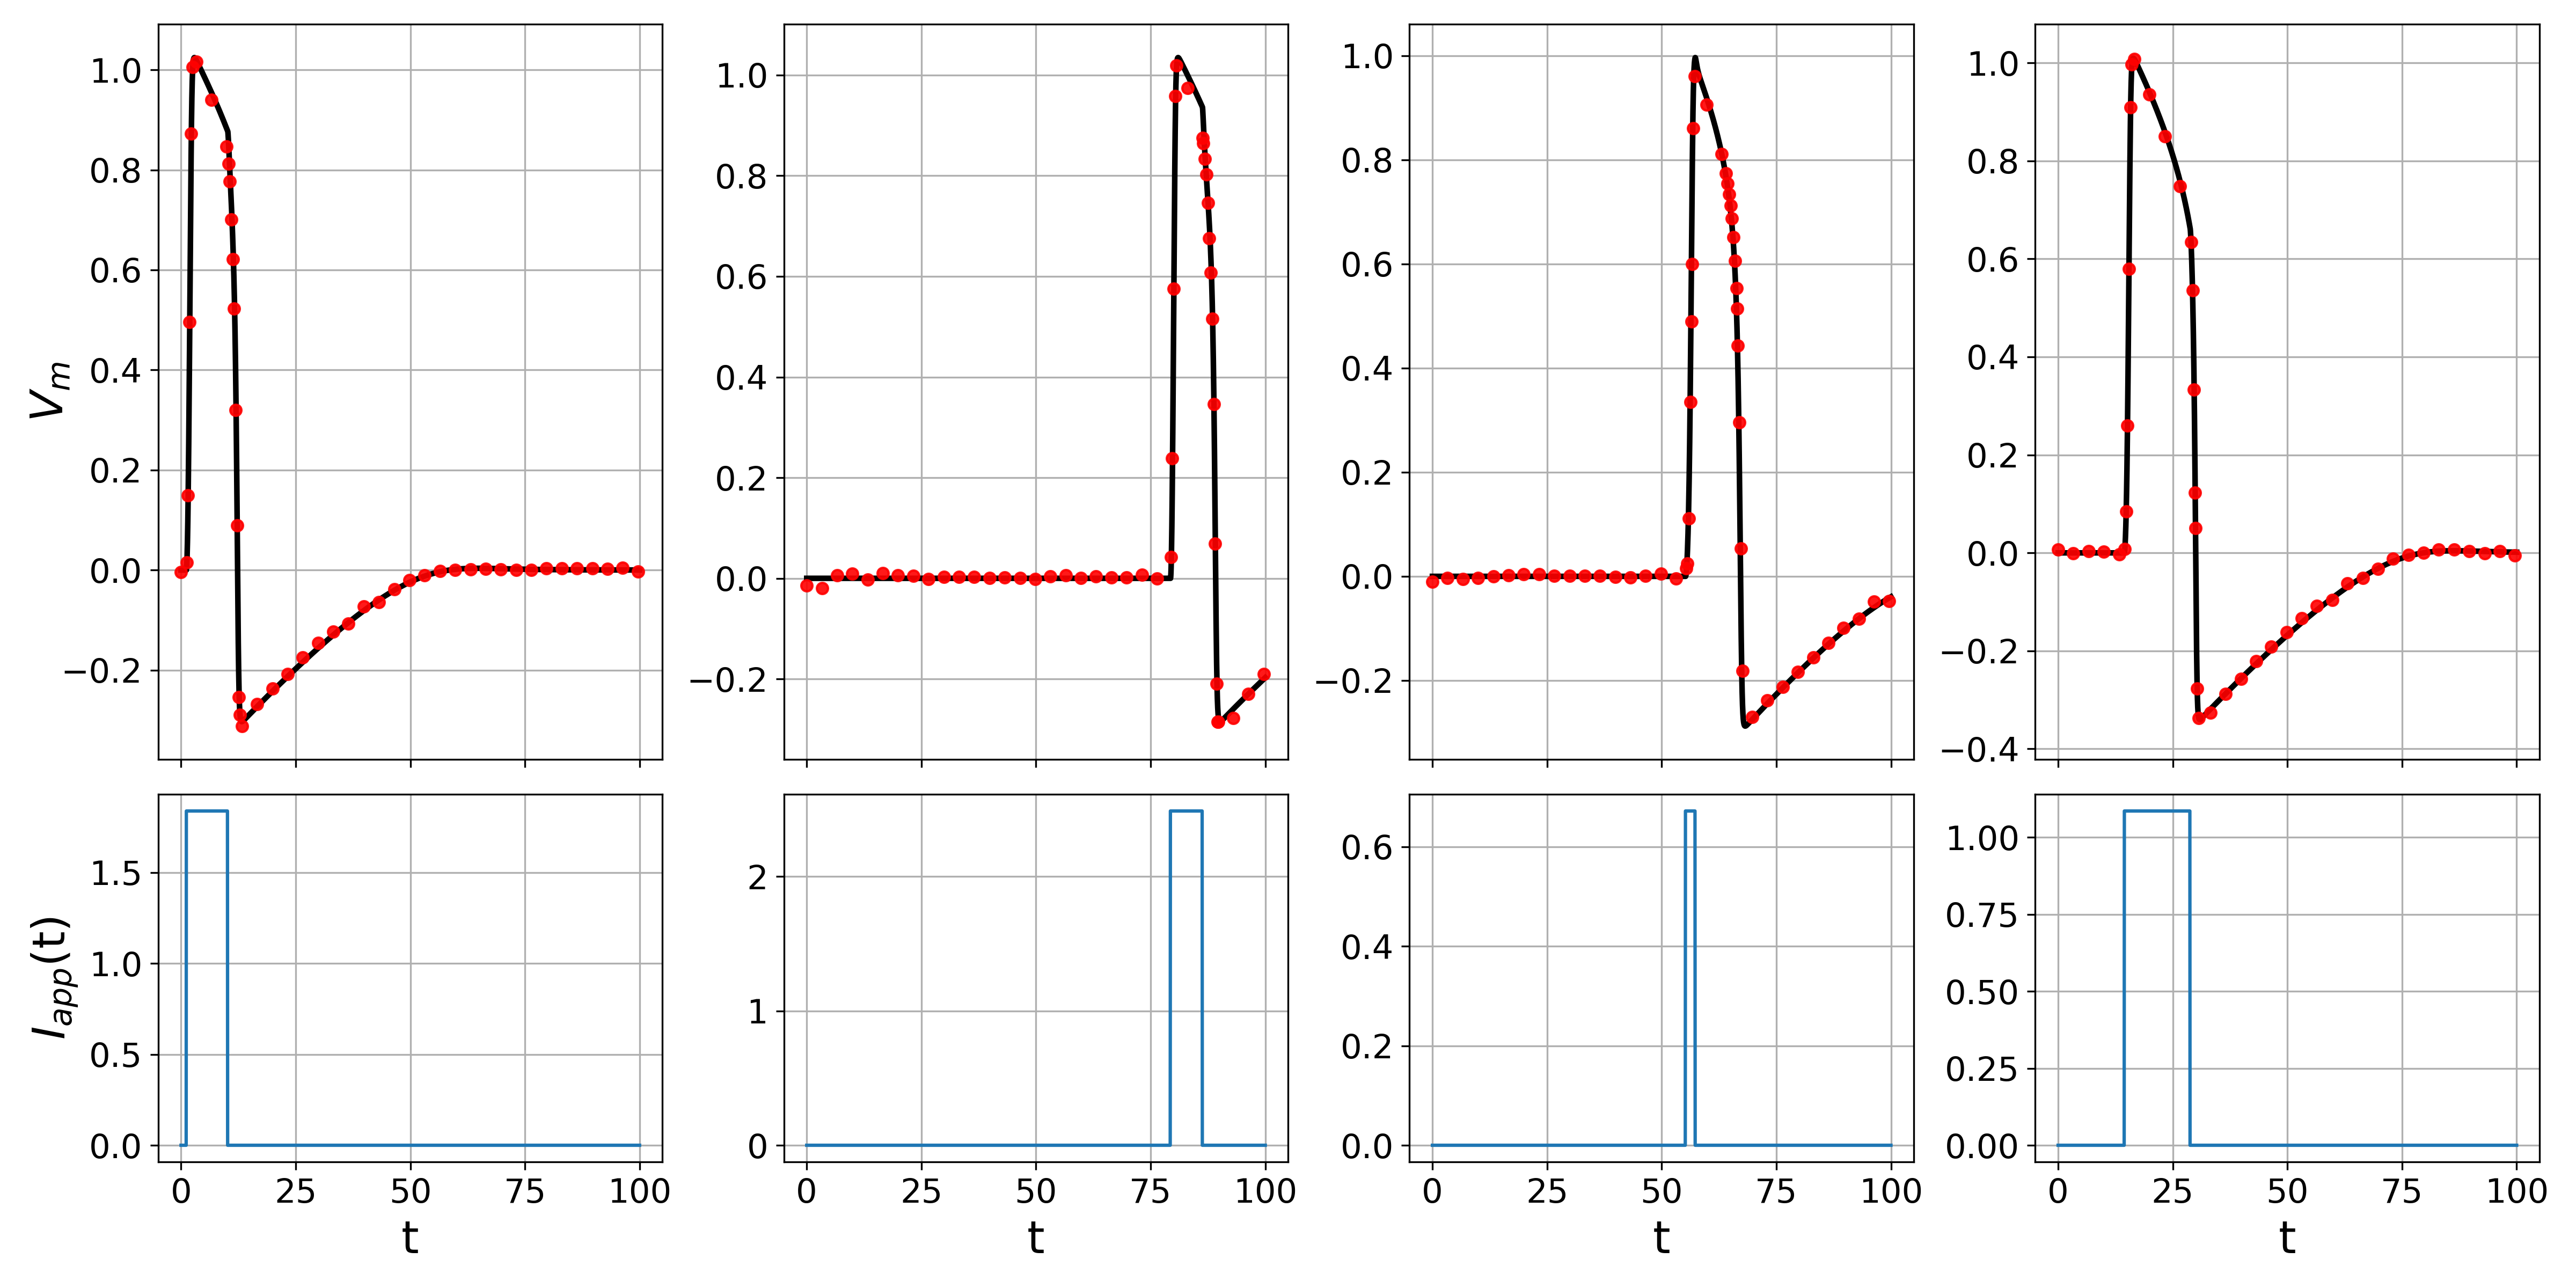
\includegraphics[width=0.7\textwidth]{img/FH_model/1to2/HHpeaks.png}
    \caption{Four instances of the test set. For each column we can see the Input current (bottom) with its corresponding potential response (top): the blue line represents the result of the simulations, whereas the dotted red line indicates the output of the NN}
    \label{fig:1to2_peaks}
\end{figure}

% --- Due figure affiancate (Loss e Istogramma L2) ---
\begin{figure}[htbp]
    \centering
    \begin{subfigure}[b]{0.48\textwidth}
        \centering
        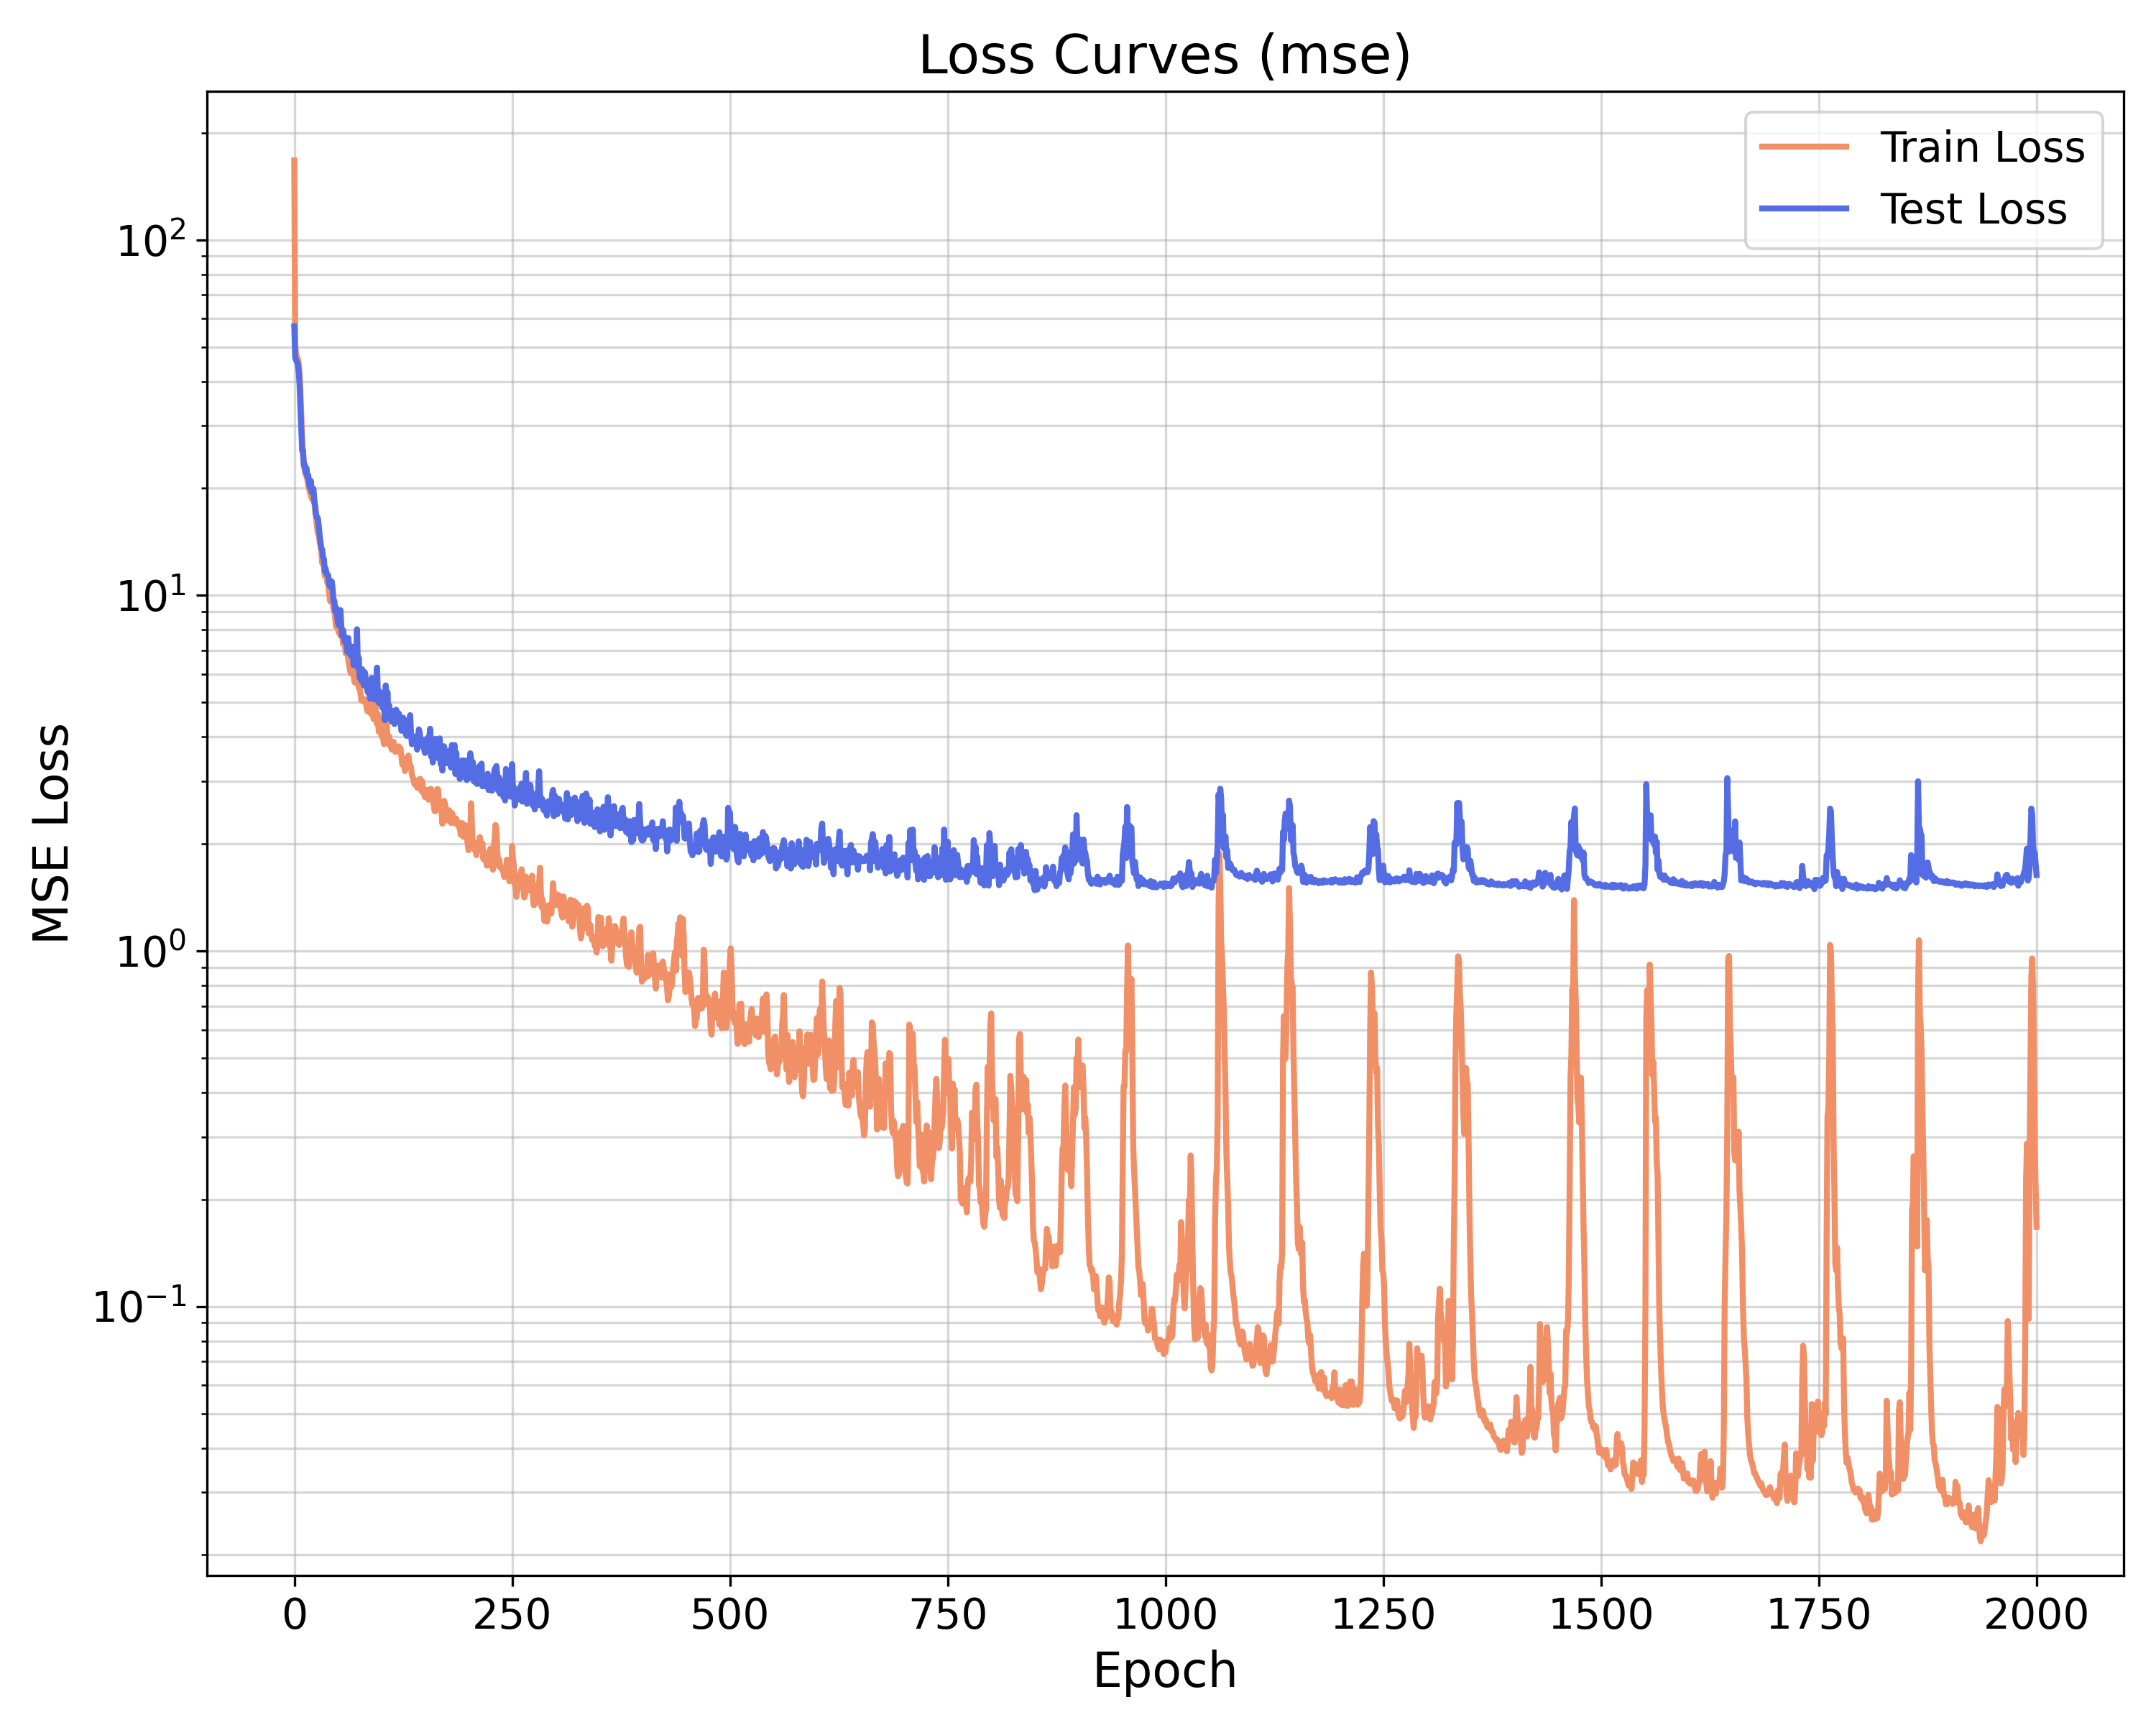
\includegraphics[width=\textwidth]{img/FH_model/1to2/loss_plot_fixed.png}
        \caption{Training and test loss}
        \label{fig:1to2_loss}
    \end{subfigure}
    \hfill
    \begin{subfigure}[b]{0.48\textwidth}
        \centering
        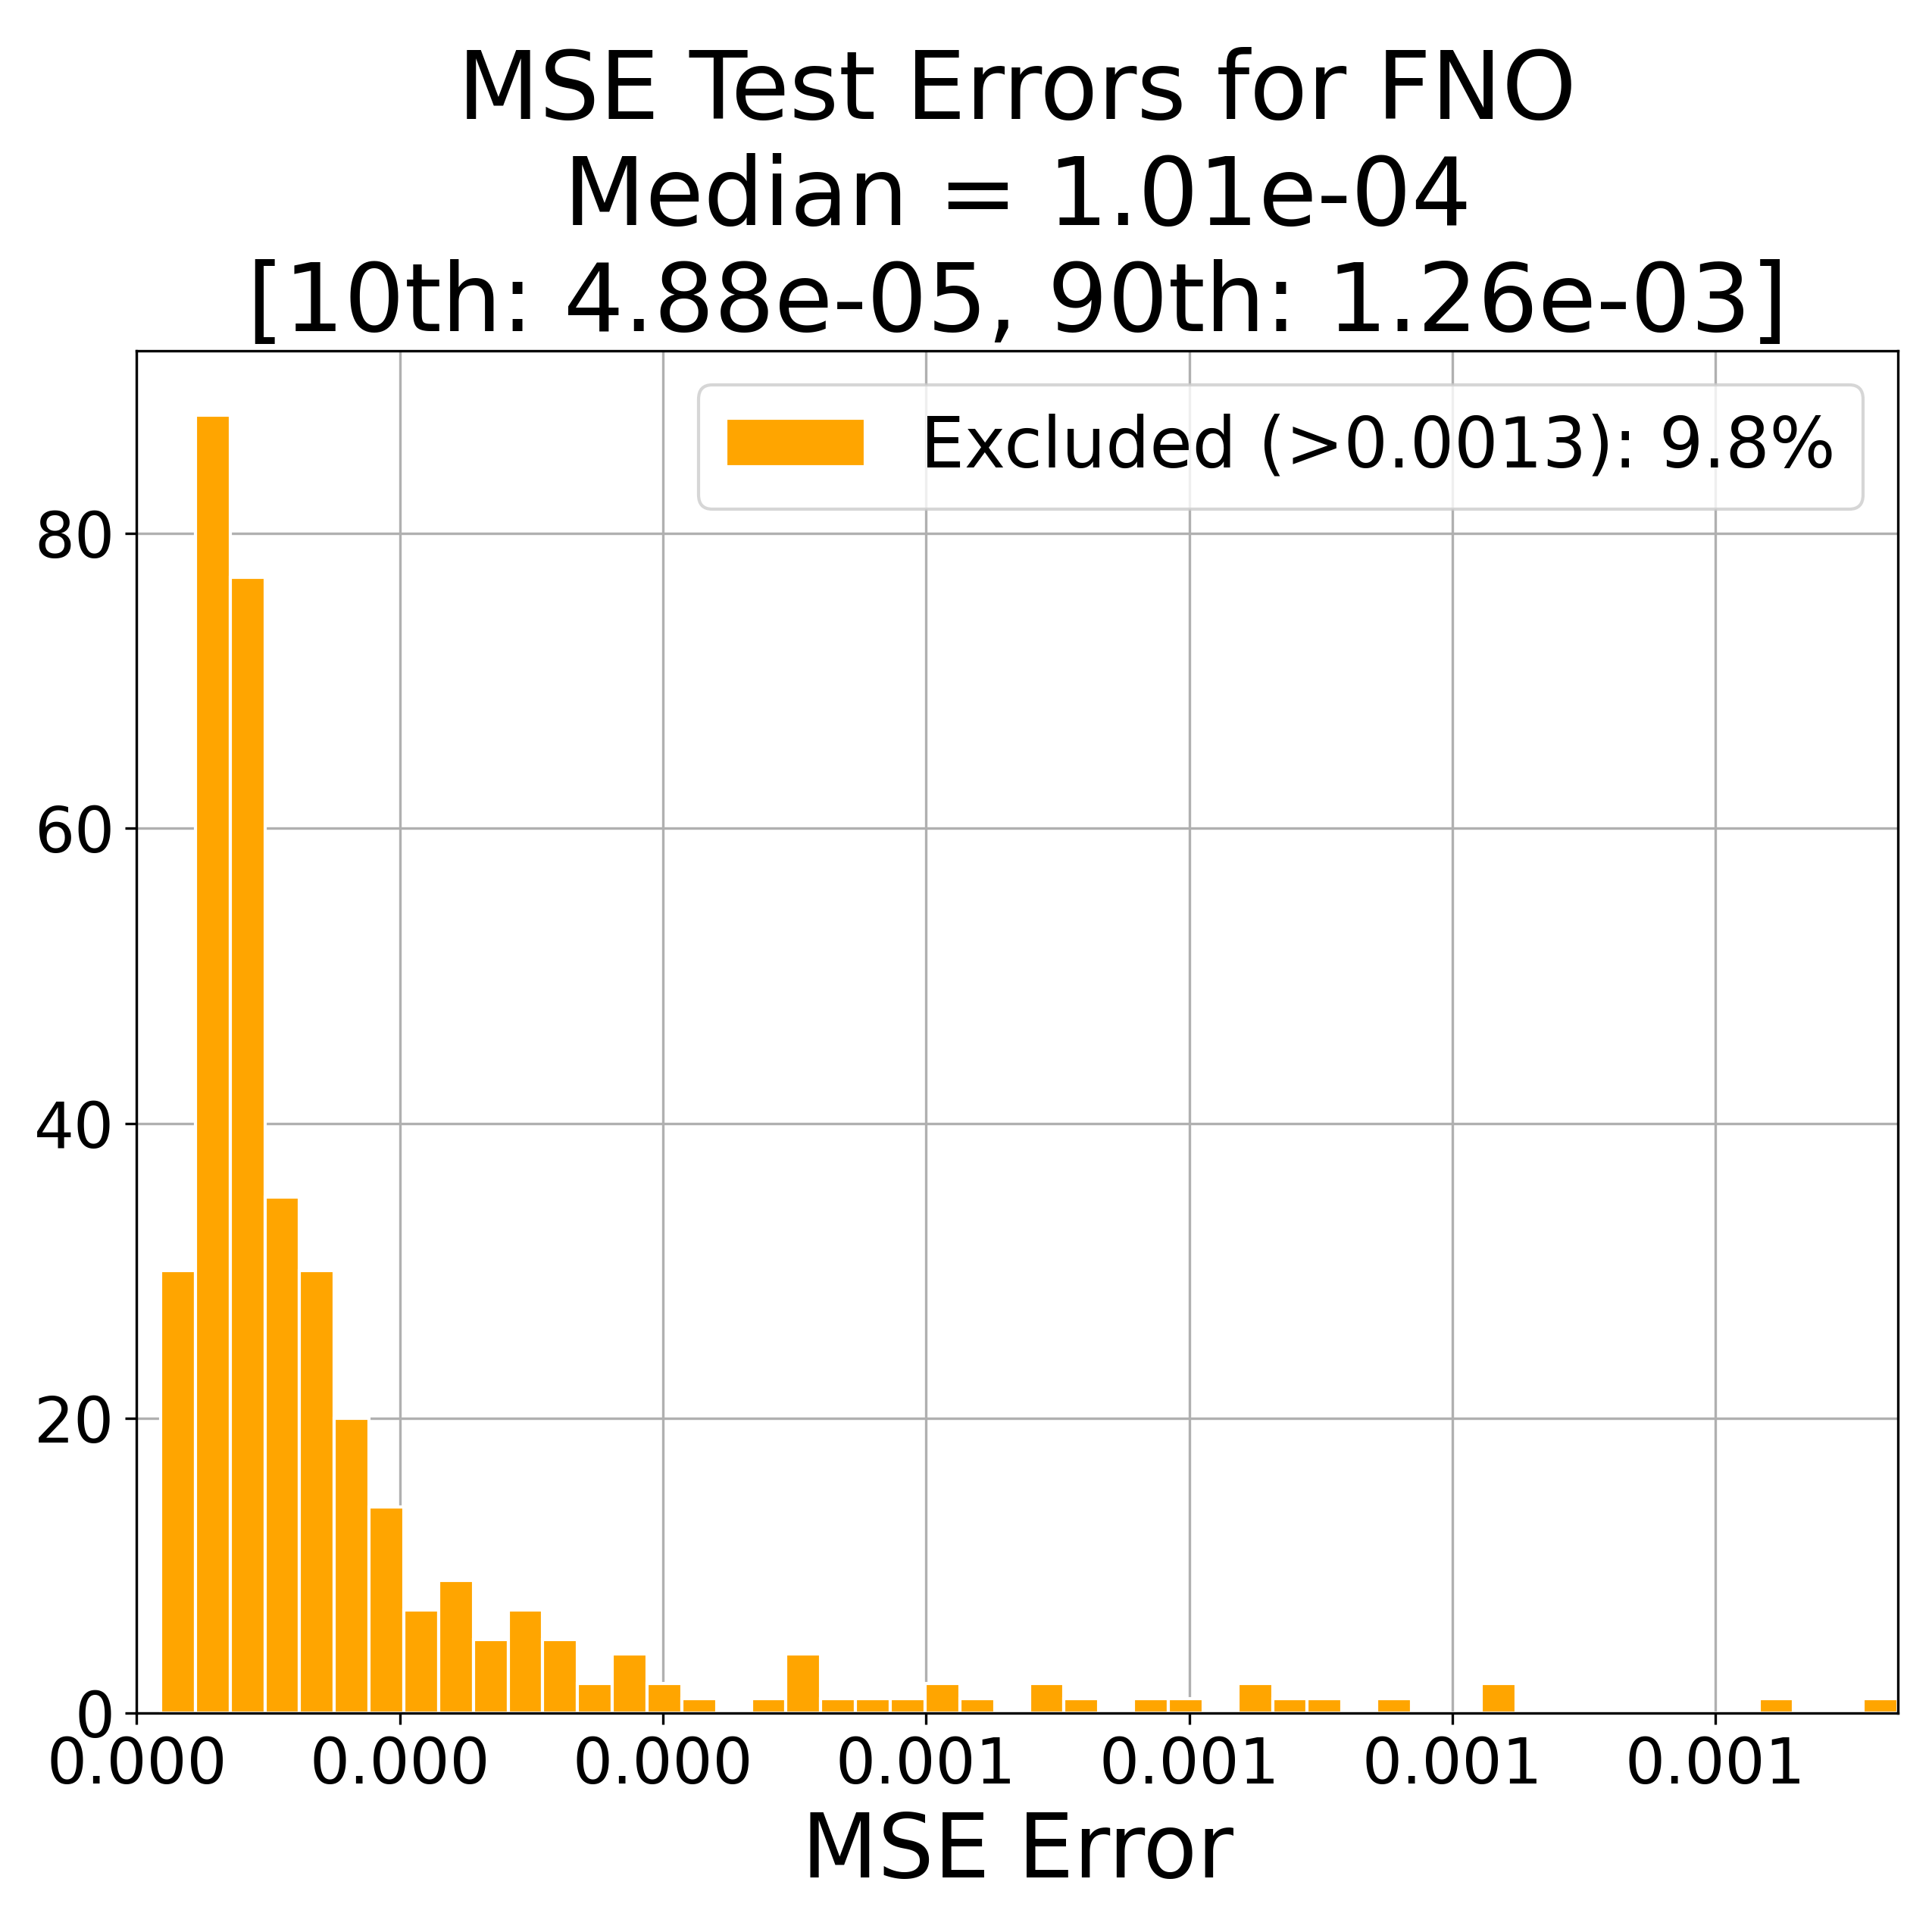
\includegraphics[width=\textwidth]{img/FH_model/1to2/L2histoFNO.png}
        \caption{MSE error distribution}
        \label{fig:1to2_l2histo}
    \end{subfigure}
    
    \caption{Loss convergence during the training process (a) and histogram of the MSE errors evaluated on the test set (b).}
    \label{fig:1to2_performance}
\end{figure}

\subsection{Toy network}
Following the same approach, we evaluated the FNO performance on a more complex spatial configuration, introducing a simple cycle topology (see fig. \ref{fig:fh_dynamics}). 

Consistent with the findings of the previous section, the network proves to be highly capable of capturing the underlying threshold dynamics. Figure \ref{fig:cycle_peaks} illustrates some instances of the test set for this new configuration. As we can see, the predicted dynamics strictly follow the numerical simulations, successfully reproducing the spiking behavior and the delay introduced by the diffusion over the cycle.

The global error metrics exhibit a behavior analogous to the "no network" scenario. As shown in Figure \ref{fig:cycle_performance}a, the training and test loss converge smoothly without any signs of overfitting. Furthermore, the MSE distribution across the test set (Figure \ref{fig:cycle_performance}b) remains tightly concentrated at very low values. This confirms that the operator learning approach is robust and its accuracy does not degrade when dealing with a small ($4$ nodes) network diffusion.

% --- Figura singola (Picchi Ciclo) ---
\begin{figure}[htbp]
    \centering
    
\includegraphics[width=0.7\textwidth]{img/FH_model/Simple_cycle/HHpeaks.png}
    \caption{Four instances of the test set for the simple cycle configuration. For each column we can see the applied input current (bottom) with its corresponding potential response (top): the blue line represents the result of the simulations, whereas the dotted red line indicates the output of the NN.}
    \label{fig:cycle_peaks}
\end{figure}

% --- Due figure affiancate (Loss e Istogramma Ciclo) ---
\begin{figure}[htbp]
    \centering
    \begin{subfigure}[b]{0.48\textwidth}
        \centering
        
\includegraphics[width=\textwidth]{img/FH_model/Simple_cycle/loss_plot_fixed.png}
        \caption{Training and test loss}
        \label{fig:cycle_loss}
    \end{subfigure}
    \hfill
    \begin{subfigure}[b]{0.48\textwidth}
        \centering
        
\includegraphics[width=\textwidth]{img/FH_model/Simple_cycle/L2histoFNO.png}
        \caption{MSE error distribution}
        \label{fig:cycle_l2histo}
    \end{subfigure}
    
    \caption{Loss convergence during the training process (a) and histogram of the MSE errors evaluated on the test set (b) for the simple cycle setup.}
    \label{fig:cycle_performance}
\end{figure}

\newpage
\subsection{ER network}
%devo fare un paragrafo in cui spiego cos'è l'ER network?
We proceeded with the study of larger networks. In particular, we wanted to observe if the performance of FNO degraded with the growing size ($N$) of the hidden network.
To conduct this experiment we performed our analysis for different size of the ER network $N= 10,100,200,300,400,500,600,700,800,900,1000,2000$ (with connection probability $p = \frac{3}{N}$).
Since the connection node for the input and output node are randomly chosen we repeated each experiments with different seeds $=0,42,100$ to distinguish if some effects are only due to chance of the particular topology/ sample of input/ output.

Here we reported only figures for the seed$=0$.

As a representative example of the system's behavior, Figure \ref{fig:er_setup_100} reports the potential dynamics for a network of size $N=100$ generated with seed $100$.

\begin{figure}[htbp]
    \centering
    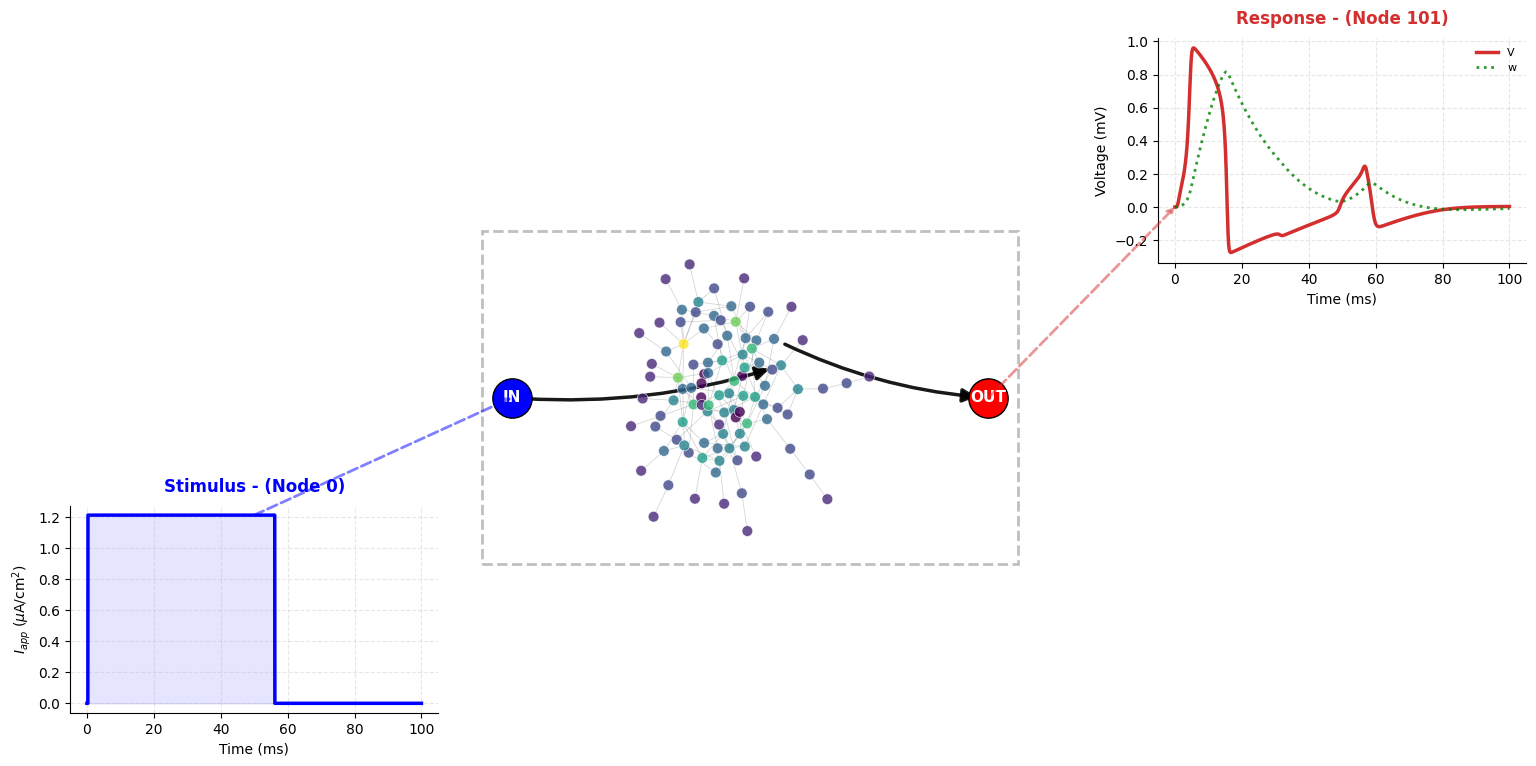
\includegraphics[width=\textwidth]{img/FH_model/ER_Network/dynamics_network_ER_N=100_seed=42.png}
    \caption{Our setup for an Erd\H{o}s-R\'enyi network of size $N=100$ (seed $100$)}
    \label{fig:er_setup_100}
\end{figure}

%%%
To systematically evaluate the threshold dynamics across all network dimensions, Figure \ref{fig:er_peaks_grid} reports the error distribution regarding the predicted number of action potential peaks for each size $N$. As we can observe from this comprehensive grid, the FNO robustly maintains its high accuracy: the vast majority of test instances exhibit zero error in the spike count, regardless of the significant increase in the network dimensionality. This confirms that the model's ability to capture the exact spiking behavior is not compromised by the growing scale of the spatial diffusion.

\begin{figure}[htbp]
    \centering
    % --- Prima riga ---
    \begin{subfigure}[b]{0.32\textwidth}
        \centering
        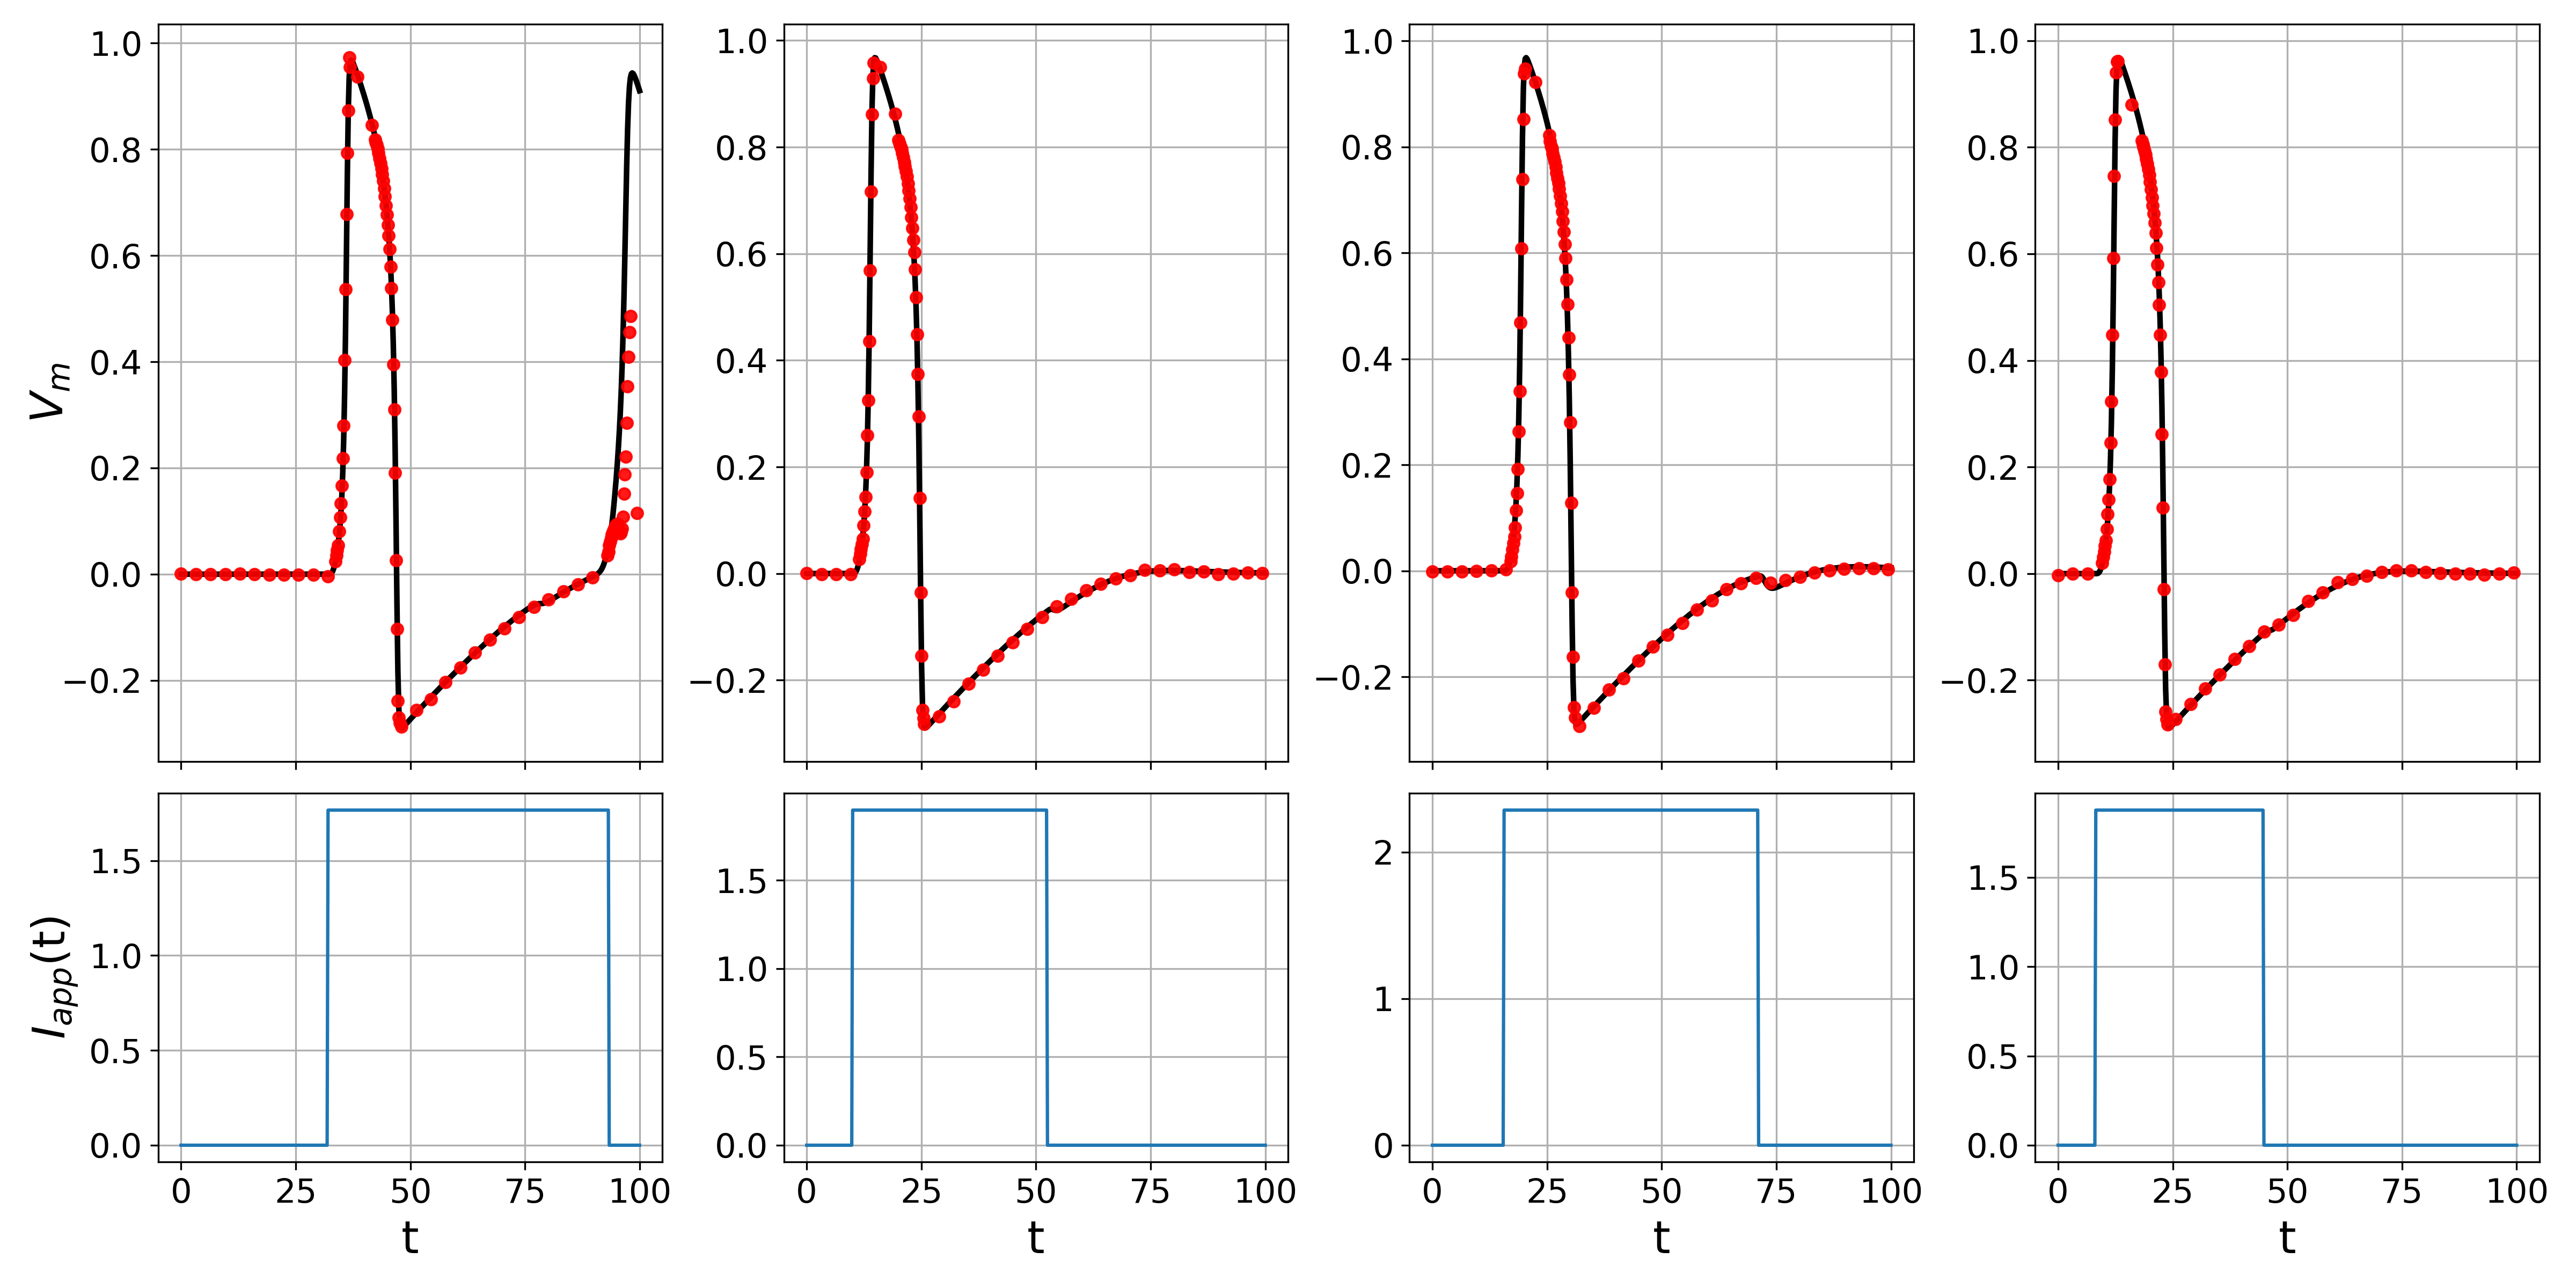
\includegraphics[width=\textwidth]{img/FH_model/ER_Network/FNO/HHpeaks_N=10.png}
        \caption{$N=10$}
    \end{subfigure}
    \hfill
    \begin{subfigure}[b]{0.32\textwidth}
        \centering
        
\includegraphics[width=\textwidth]{img/FH_model/ER_Network/FNO/HHpeaks_N=100.png}
        \caption{$N=100$}
    \end{subfigure}
    \hfill
    \begin{subfigure}[b]{0.32\textwidth}
        \centering
        
\includegraphics[width=\textwidth]{img/FH_model/ER_Network/FNO/HHpeaks_N=200.png}
        \caption{$N=200$}
    \end{subfigure}
    
    \vspace{0.4cm} % Spazio verticale tra le righe
    
    % --- Seconda riga ---
    \begin{subfigure}[b]{0.32\textwidth}
        \centering
        
\includegraphics[width=\textwidth]{img/FH_model/ER_Network/FNO/HHpeaks_N=300.png}
        \caption{$N=300$}
    \end{subfigure}
    \hfill
    \begin{subfigure}[b]{0.32\textwidth}
        \centering
        
\includegraphics[width=\textwidth]{img/FH_model/ER_Network/FNO/HHpeaks_N=400.png}
        \caption{$N=400$}
    \end{subfigure}
    \hfill
    \begin{subfigure}[b]{0.32\textwidth}
        \centering
        
\includegraphics[width=\textwidth]{img/FH_model/ER_Network/FNO/HHpeaks_N=500.png}
        \caption{$N=500$}
    \end{subfigure}
    
    \vspace{0.4cm}
    
    % --- Terza riga ---
    \begin{subfigure}[b]{0.32\textwidth}
        \centering
        
\includegraphics[width=\textwidth]{img/FH_model/ER_Network/FNO/HHpeaks_N=600.png}
        \caption{$N=600$}
    \end{subfigure}
    \hfill
    \begin{subfigure}[b]{0.32\textwidth}
        \centering
        
\includegraphics[width=\textwidth]{img/FH_model/ER_Network/FNO/HHpeaks_N=700.png}
        \caption{$N=700$}
    \end{subfigure}
    \hfill
    \begin{subfigure}[b]{0.32\textwidth}
        \centering
        
\includegraphics[width=\textwidth]{img/FH_model/ER_Network/FNO/HHpeaks_N=800.png}
        \caption{$N=800$}
    \end{subfigure}
    
    \vspace{0.4cm}
    
    % --- Quarta riga ---
    \begin{subfigure}[b]{0.32\textwidth}
        \centering
        
\includegraphics[width=\textwidth]{img/FH_model/ER_Network/FNO/HHpeaks_N=900.png}
        \caption{$N=900$}
    \end{subfigure}
    \hfill
    \begin{subfigure}[b]{0.32\textwidth}
        \centering
        
\includegraphics[width=\textwidth]{img/FH_model/ER_Network/FNO/HHpeaks_N=1000.png}
        \caption{$N=1000$}
    \end{subfigure}
    \hfill
    \begin{subfigure}[b]{0.32\textwidth}
        \centering
        
\includegraphics[width=\textwidth]{img/FH_model/ER_Network/FNO/HHpeaks_N=2000.png}
        \caption{$N=2000$}
    \end{subfigure}
    
    \caption{Some instances of the test set for different Erd\H{o}s-R\'enyi network sizes ($N$).  For each column we can see the applied input current (bottom) with its corresponding potential response (top): the blue line represents the result of the simulations, whereas the dotted red line indicates the output of the NN.}
    \label{fig:er_peaks_grid}
\end{figure}


%%%
% ==========================================
% GRIGLIA 1: MSE HISTOGRAMS

%Devo rifarli ? alcune cifre sull'asse x si sovrappongono e forse dovrei usare la notazione scientifica per Mean=. ???
% ==========================================

\begin{figure}[htbp]
    \centering
    % --- Prima riga ---
    \begin{subfigure}[b]{0.32\textwidth}
        \centering
        
\includegraphics[width=\textwidth]{img/FH_model/ER_Network/FNO/L2histoFNO_N=10.png}
        \caption{$N=10$}
    \end{subfigure}
    \hfill
    \begin{subfigure}[b]{0.32\textwidth}
        \centering
        
\includegraphics[width=\textwidth]{img/FH_model/ER_Network/FNO/L2histoFNO_N=100.png}
        \caption{$N=100$}
    \end{subfigure}
    \hfill
    \begin{subfigure}[b]{0.32\textwidth}
        \centering
        
\includegraphics[width=\textwidth]{img/FH_model/ER_Network/FNO/L2histoFNO_N=200.png}
        \caption{$N=200$}
    \end{subfigure}
    
    \vspace{0.4cm}
    
    % --- Seconda riga ---
    \begin{subfigure}[b]{0.32\textwidth}
        \centering
        
\includegraphics[width=\textwidth]{img/FH_model/ER_Network/FNO/L2histoFNO_N=300.png}
        \caption{$N=300$}
    \end{subfigure}
    \hfill
    \begin{subfigure}[b]{0.32\textwidth}
        \centering
        
\includegraphics[width=\textwidth]{img/FH_model/ER_Network/FNO/L2histoFNO_N=400.png}
        \caption{$N=400$}
    \end{subfigure}
    \hfill
    \begin{subfigure}[b]{0.32\textwidth}
        \centering
        
\includegraphics[width=\textwidth]{img/FH_model/ER_Network/FNO/L2histoFNO_N=500.png}
        \caption{$N=500$}
    \end{subfigure}
    
    \vspace{0.4cm}
    
    % --- Terza riga ---
    \begin{subfigure}[b]{0.32\textwidth}
        \centering
        
\includegraphics[width=\textwidth]{img/FH_model/ER_Network/FNO/L2histoFNO_N=600.png}
        \caption{$N=600$}
    \end{subfigure}
    \hfill
    \begin{subfigure}[b]{0.32\textwidth}
        \centering
        
\includegraphics[width=\textwidth]{img/FH_model/ER_Network/FNO/L2histoFNO_N=700.png}
        \caption{$N=700$}
    \end{subfigure}
    \hfill
    \begin{subfigure}[b]{0.32\textwidth}
        \centering
        
\includegraphics[width=\textwidth]{img/FH_model/ER_Network/FNO/L2histoFNO_N=800.png}
        \caption{$N=800$}
    \end{subfigure}
    
    \vspace{0.4cm}
    
    % --- Quarta riga ---
    \begin{subfigure}[b]{0.32\textwidth}
        \centering
        
\includegraphics[width=\textwidth]{img/FH_model/ER_Network/FNO/L2histoFNO_N=900.png}
        \caption{$N=900$}
    \end{subfigure}
    \hfill
    \begin{subfigure}[b]{0.32\textwidth}
        \centering
        
\includegraphics[width=\textwidth]{img/FH_model/ER_Network/FNO/L2histoFNO_N=1000.png}
        \caption{$N=1000$}
    \end{subfigure}
    \hfill
    \begin{subfigure}[b]{0.32\textwidth}
        \centering
        
\includegraphics[width=\textwidth]{img/FH_model/ER_Network/FNO/L2histoFNO_N=2000.png}
        \caption{$N=2000$}
    \end{subfigure}
    
    \caption{MSE error distributions across the test set for different Erd\H{o}s-R\'enyi network sizes ($N$).}
    \label{fig:er_histo_grid}
\end{figure}

% ==========================================
% GRIGLIA 2: LOSS PLOTS
% ==========================================
\begin{figure}[htbp]
    \centering
    % --- Prima riga ---
    \begin{subfigure}[b]{0.32\textwidth}
        \centering
        
\includegraphics[width=\textwidth]{img/FH_model/ER_Network/FNO/loss_plot_fixed_N=10.png}
        \caption{$N=10$}
    \end{subfigure}
    \hfill
    \begin{subfigure}[b]{0.32\textwidth}
        \centering
        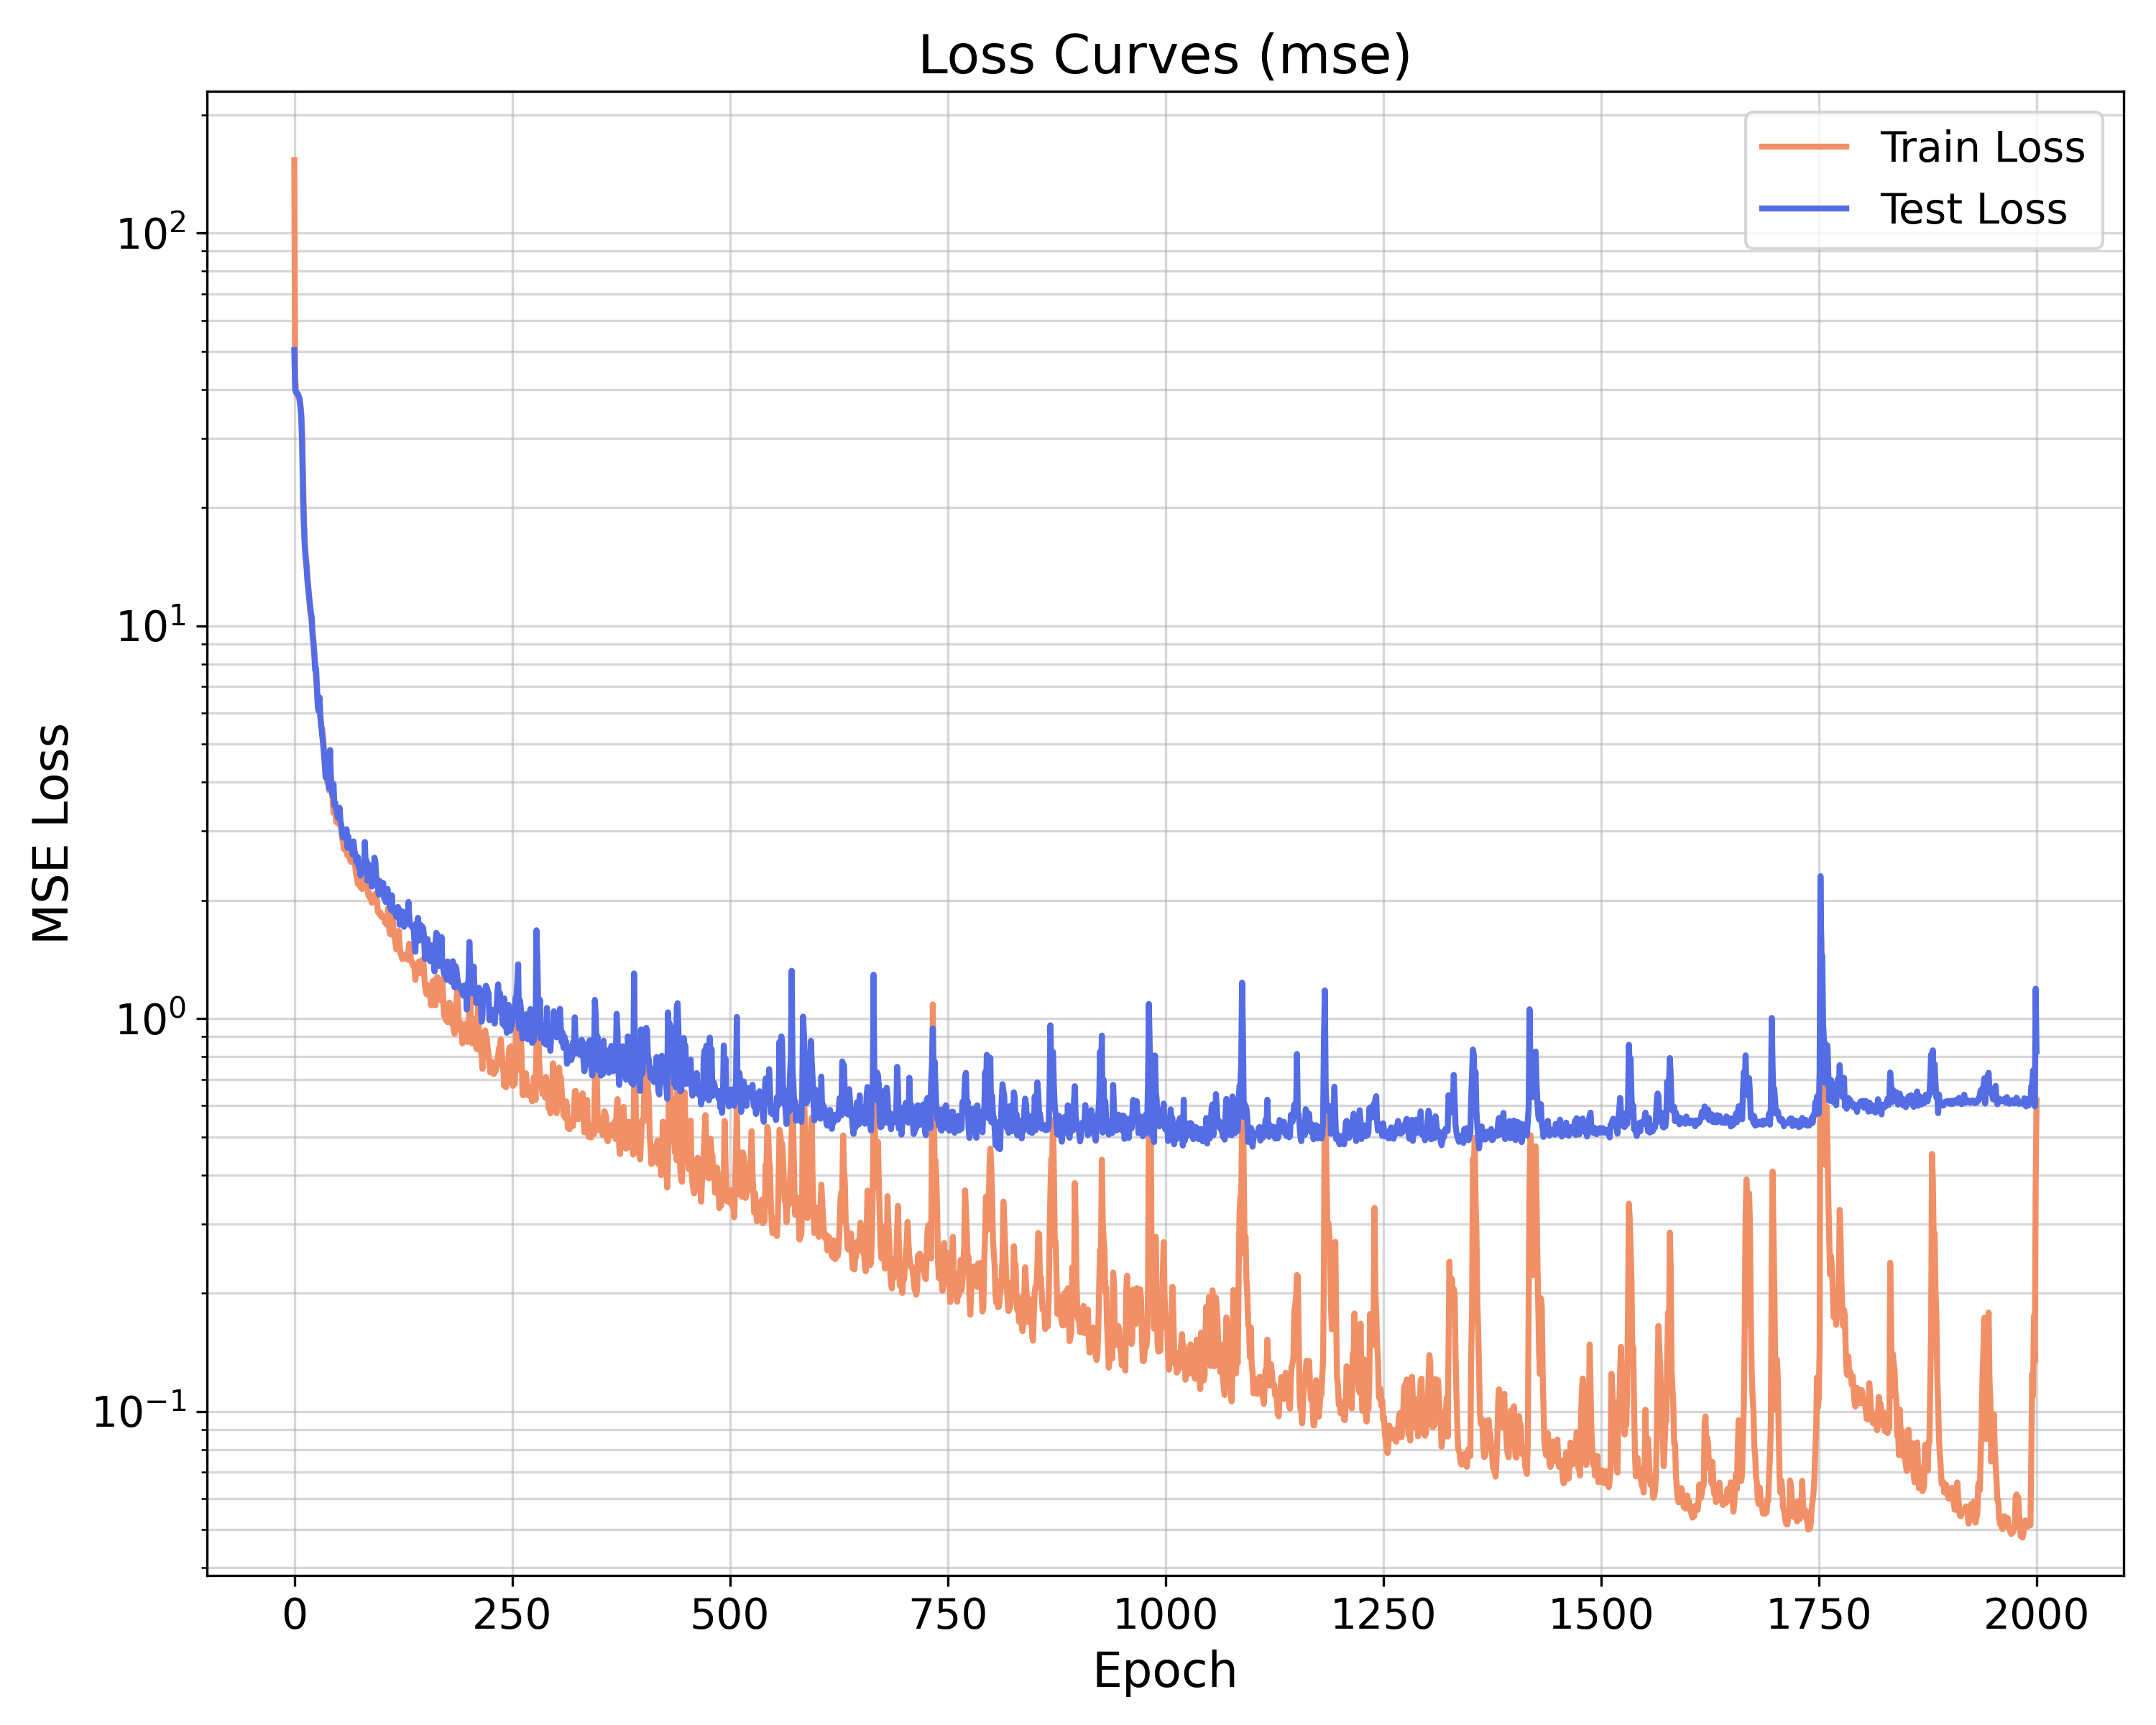
\includegraphics[width=\textwidth]{img/FH_model/ER_Network/FNO/loss_plot_fixed_N=100.png}
        \caption{$N=100$}
    \end{subfigure}
    \hfill
    \begin{subfigure}[b]{0.32\textwidth}
        \centering
        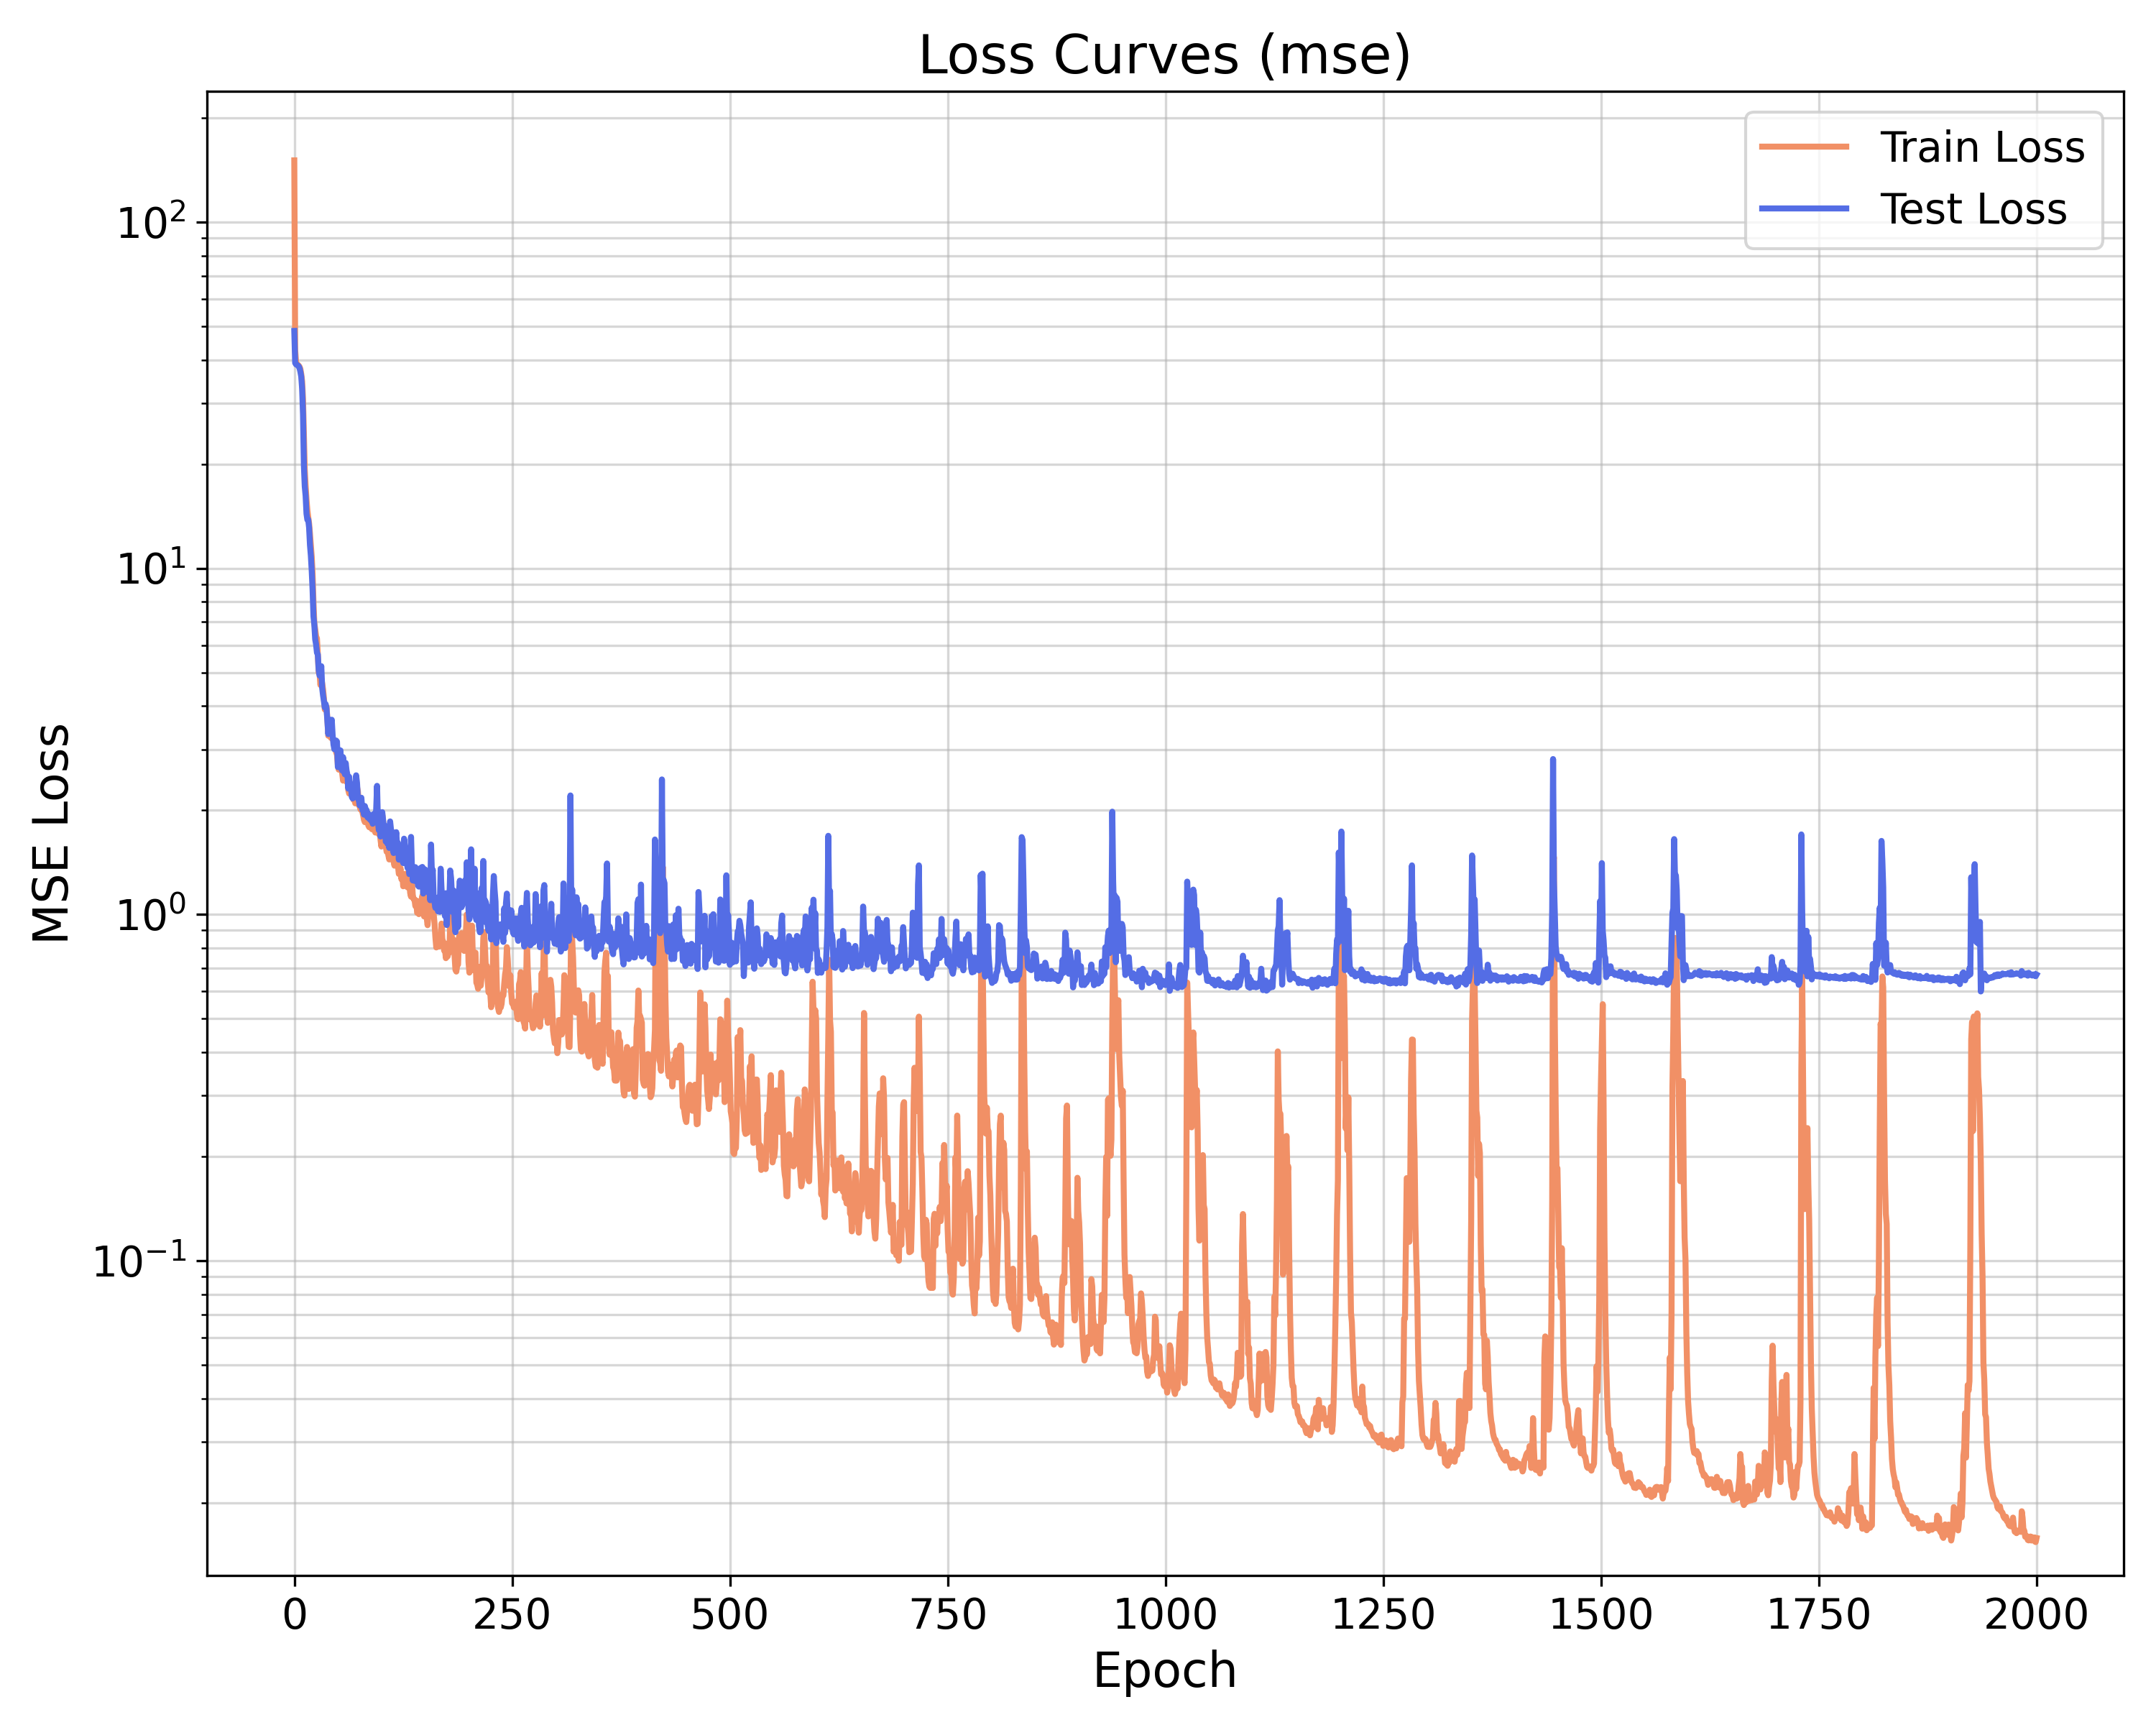
\includegraphics[width=\textwidth]{img/FH_model/ER_Network/FNO/loss_plot_fixed_N=200.png}
        \caption{$N=200$}
    \end{subfigure}
    
    \vspace{0.4cm}
    
    % --- Seconda riga ---
    \begin{subfigure}[b]{0.32\textwidth}
        \centering
        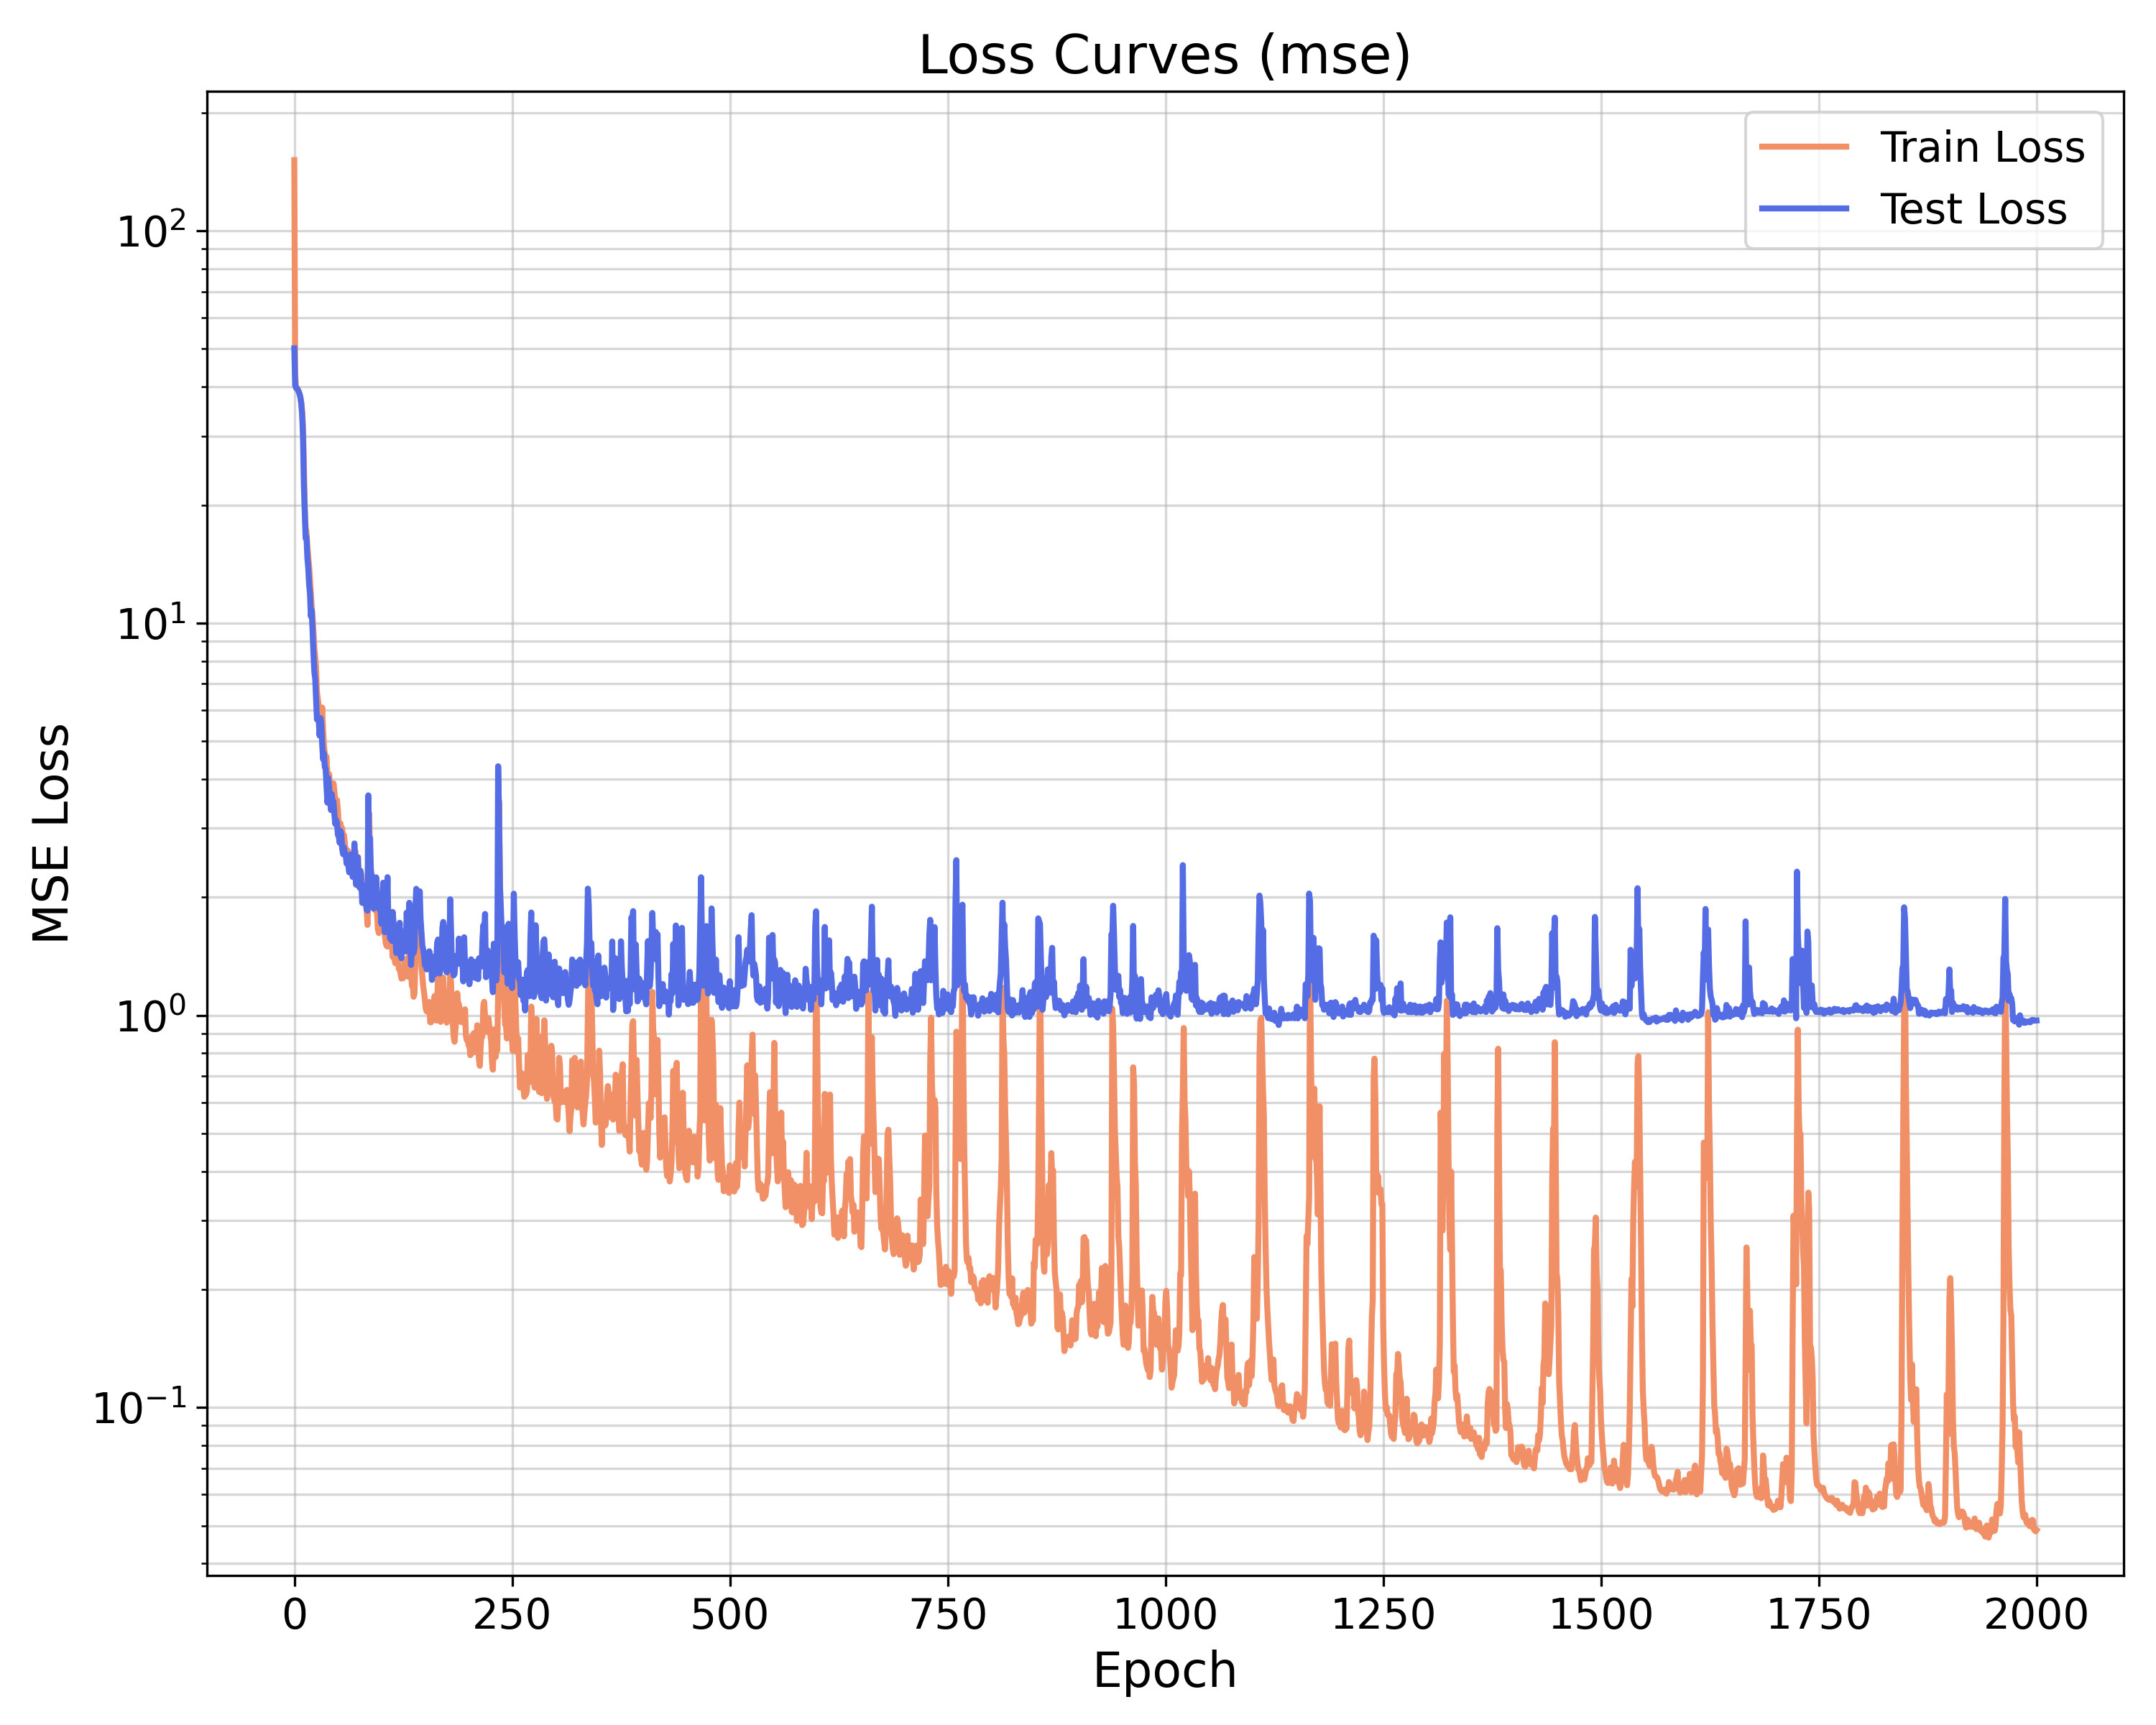
\includegraphics[width=\textwidth]{img/FH_model/ER_Network/FNO/loss_plot_fixed_N=300.png}
        \caption{$N=300$}
    \end{subfigure}
    \hfill
    \begin{subfigure}[b]{0.32\textwidth}
        \centering
        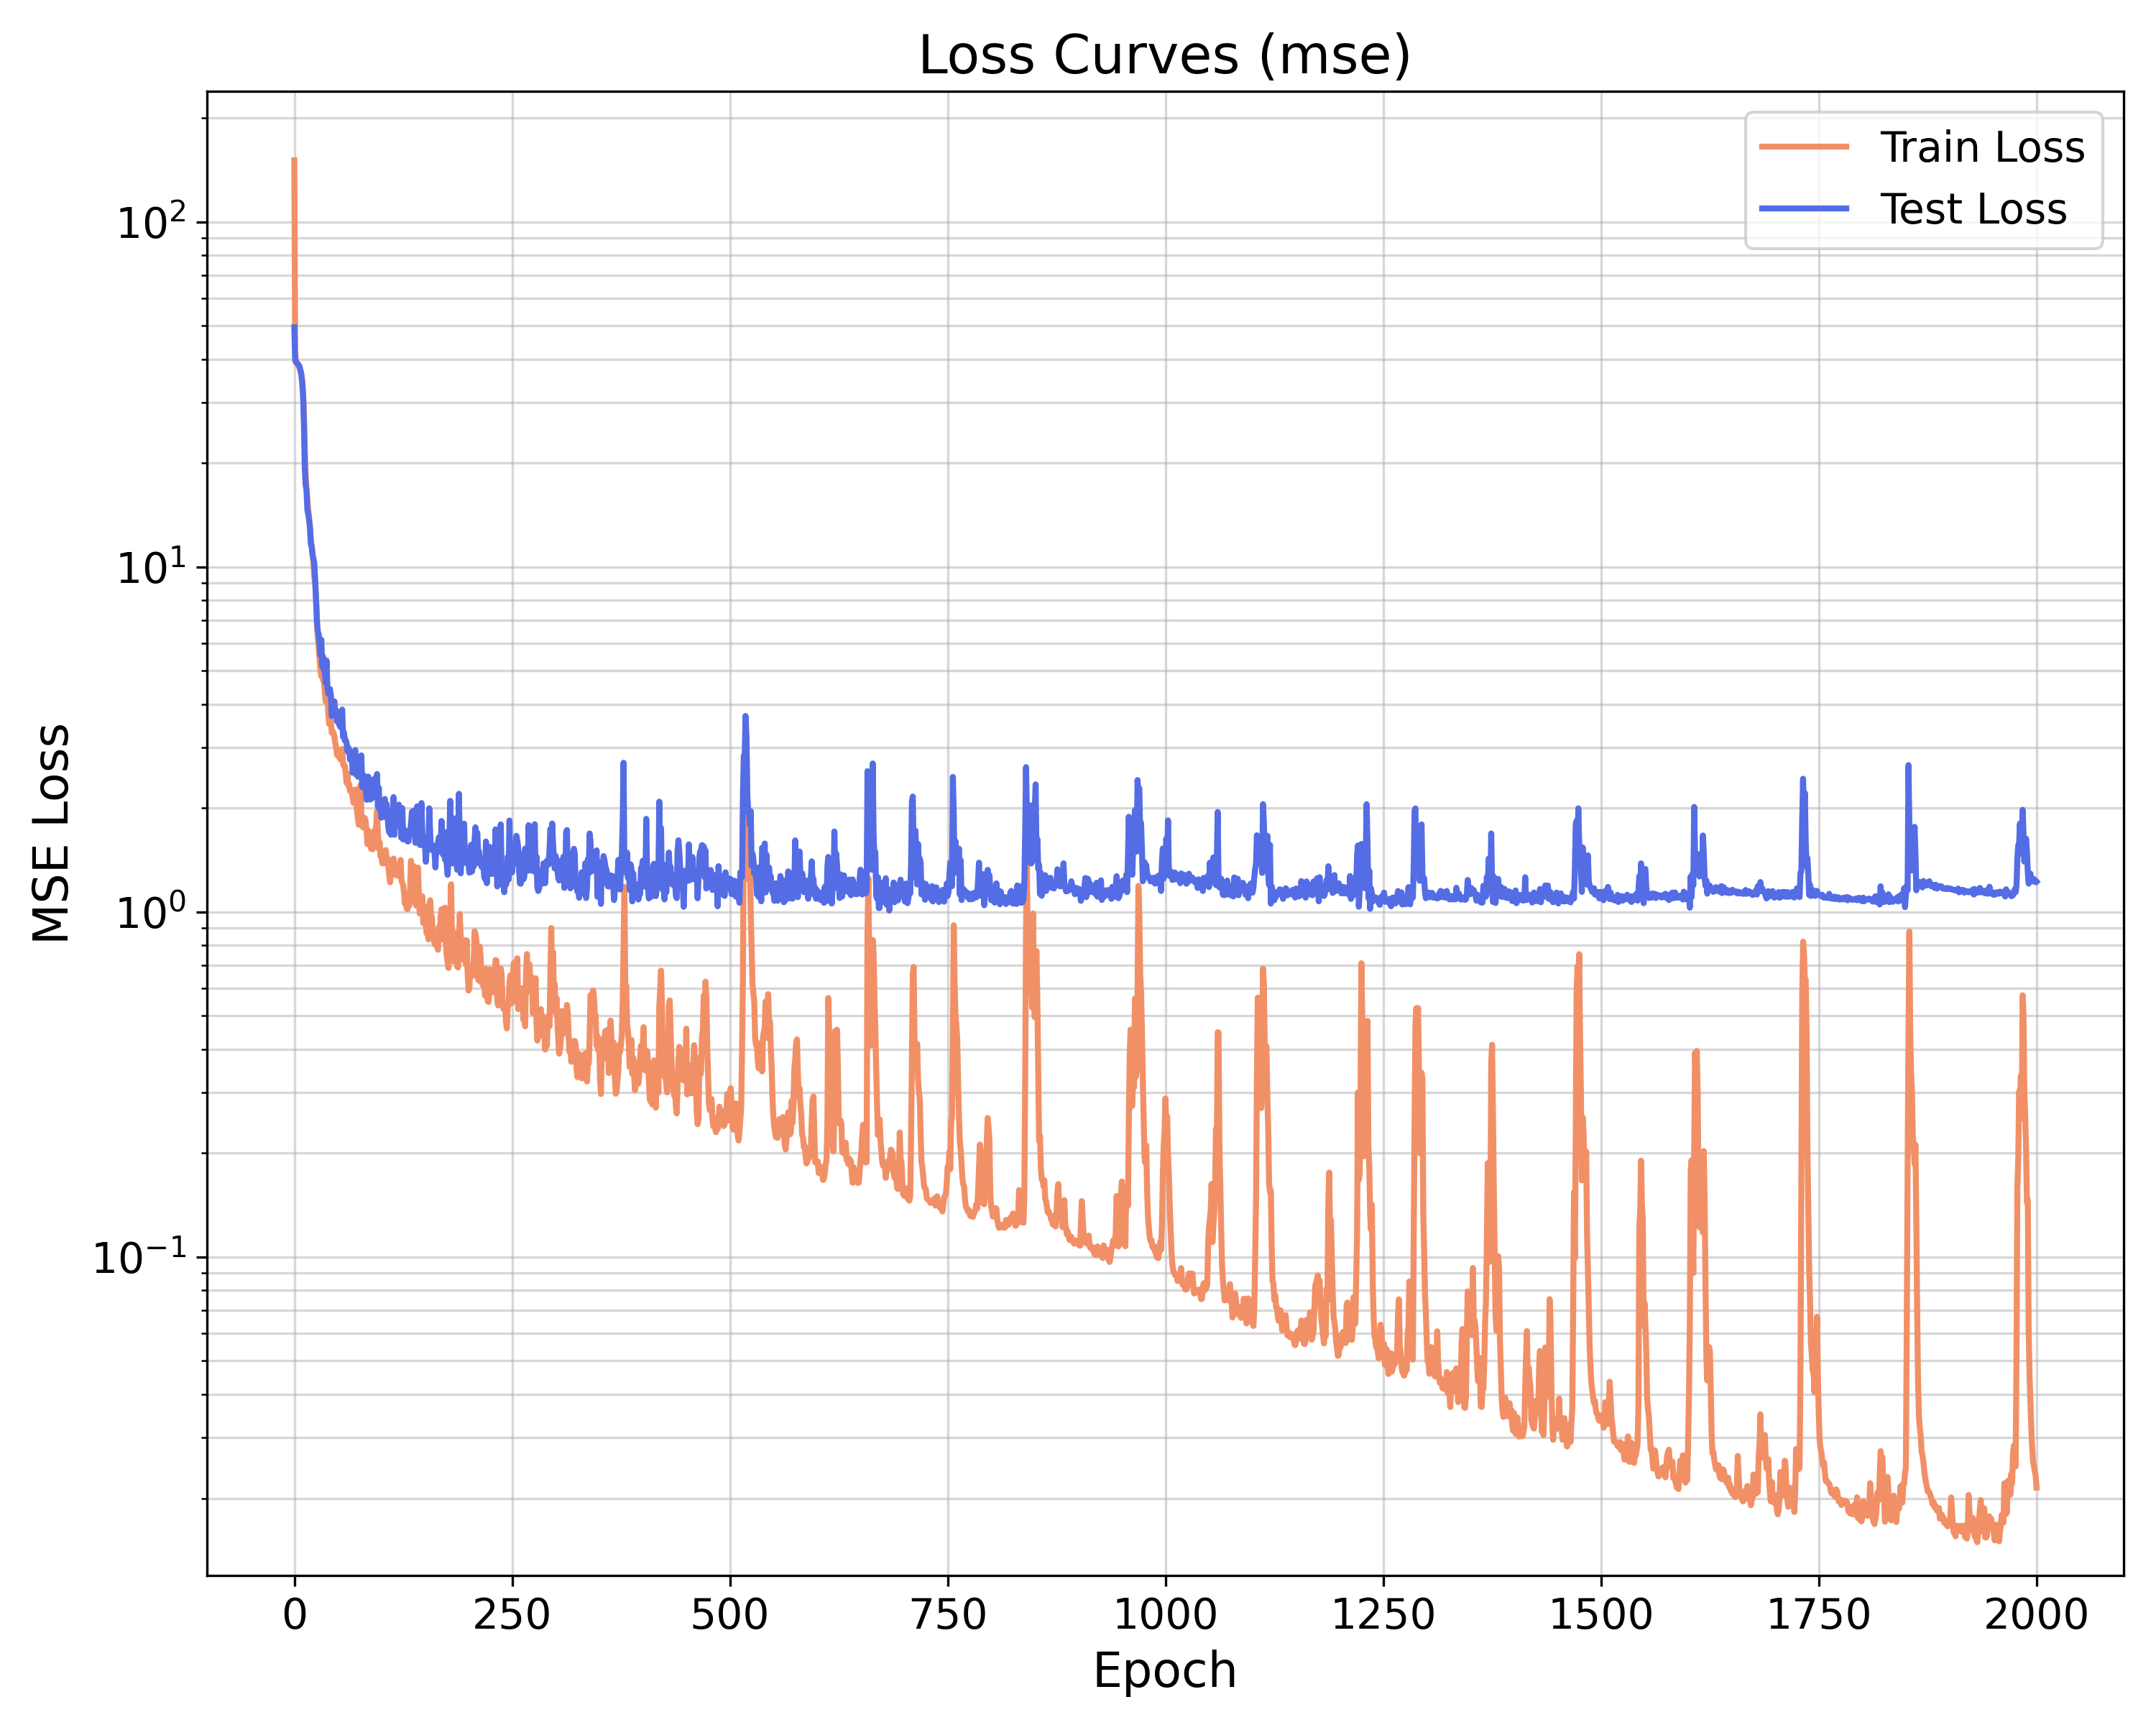
\includegraphics[width=\textwidth]{img/FH_model/ER_Network/FNO/loss_plot_fixed_N=400.png}
        \caption{$N=400$}
    \end{subfigure}
    \hfill
    \begin{subfigure}[b]{0.32\textwidth}
        \centering
        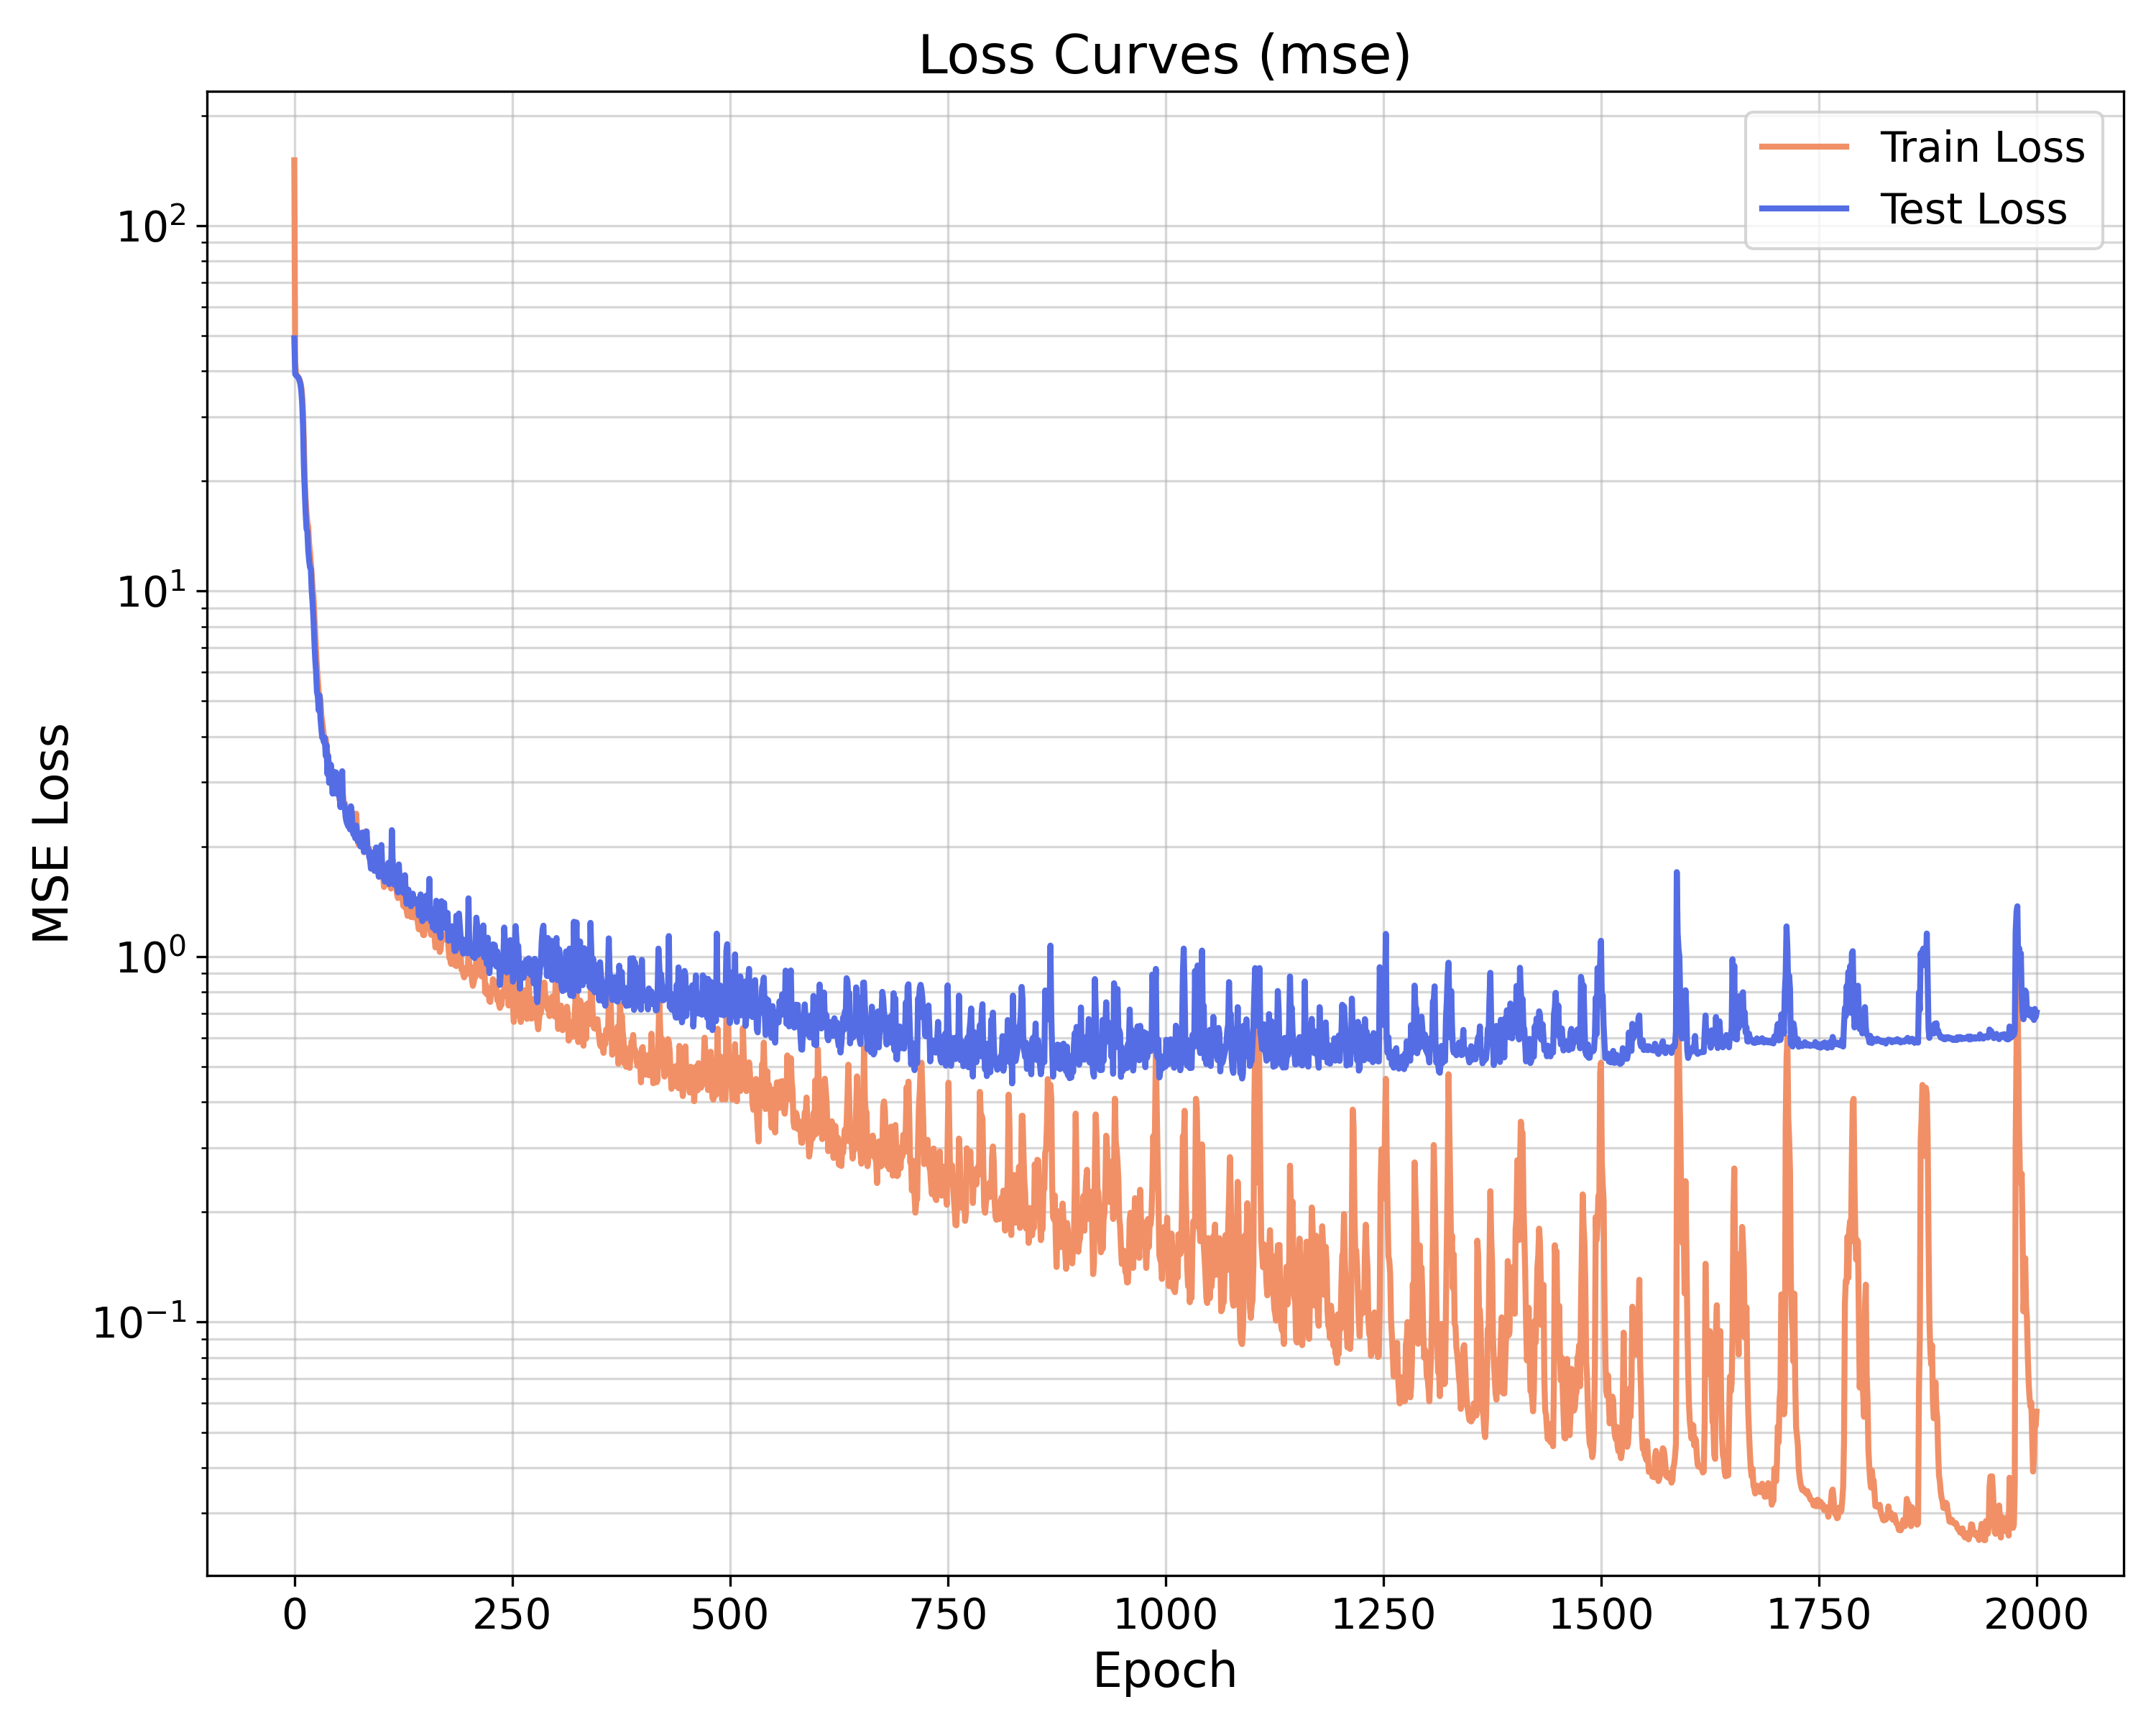
\includegraphics[width=\textwidth]{img/FH_model/ER_Network/FNO/loss_plot_fixed_N=500.png}
        \caption{$N=500$}
    \end{subfigure}
    
    \vspace{0.4cm}
    
    % --- Terza riga ---
    \begin{subfigure}[b]{0.32\textwidth}
        \centering
        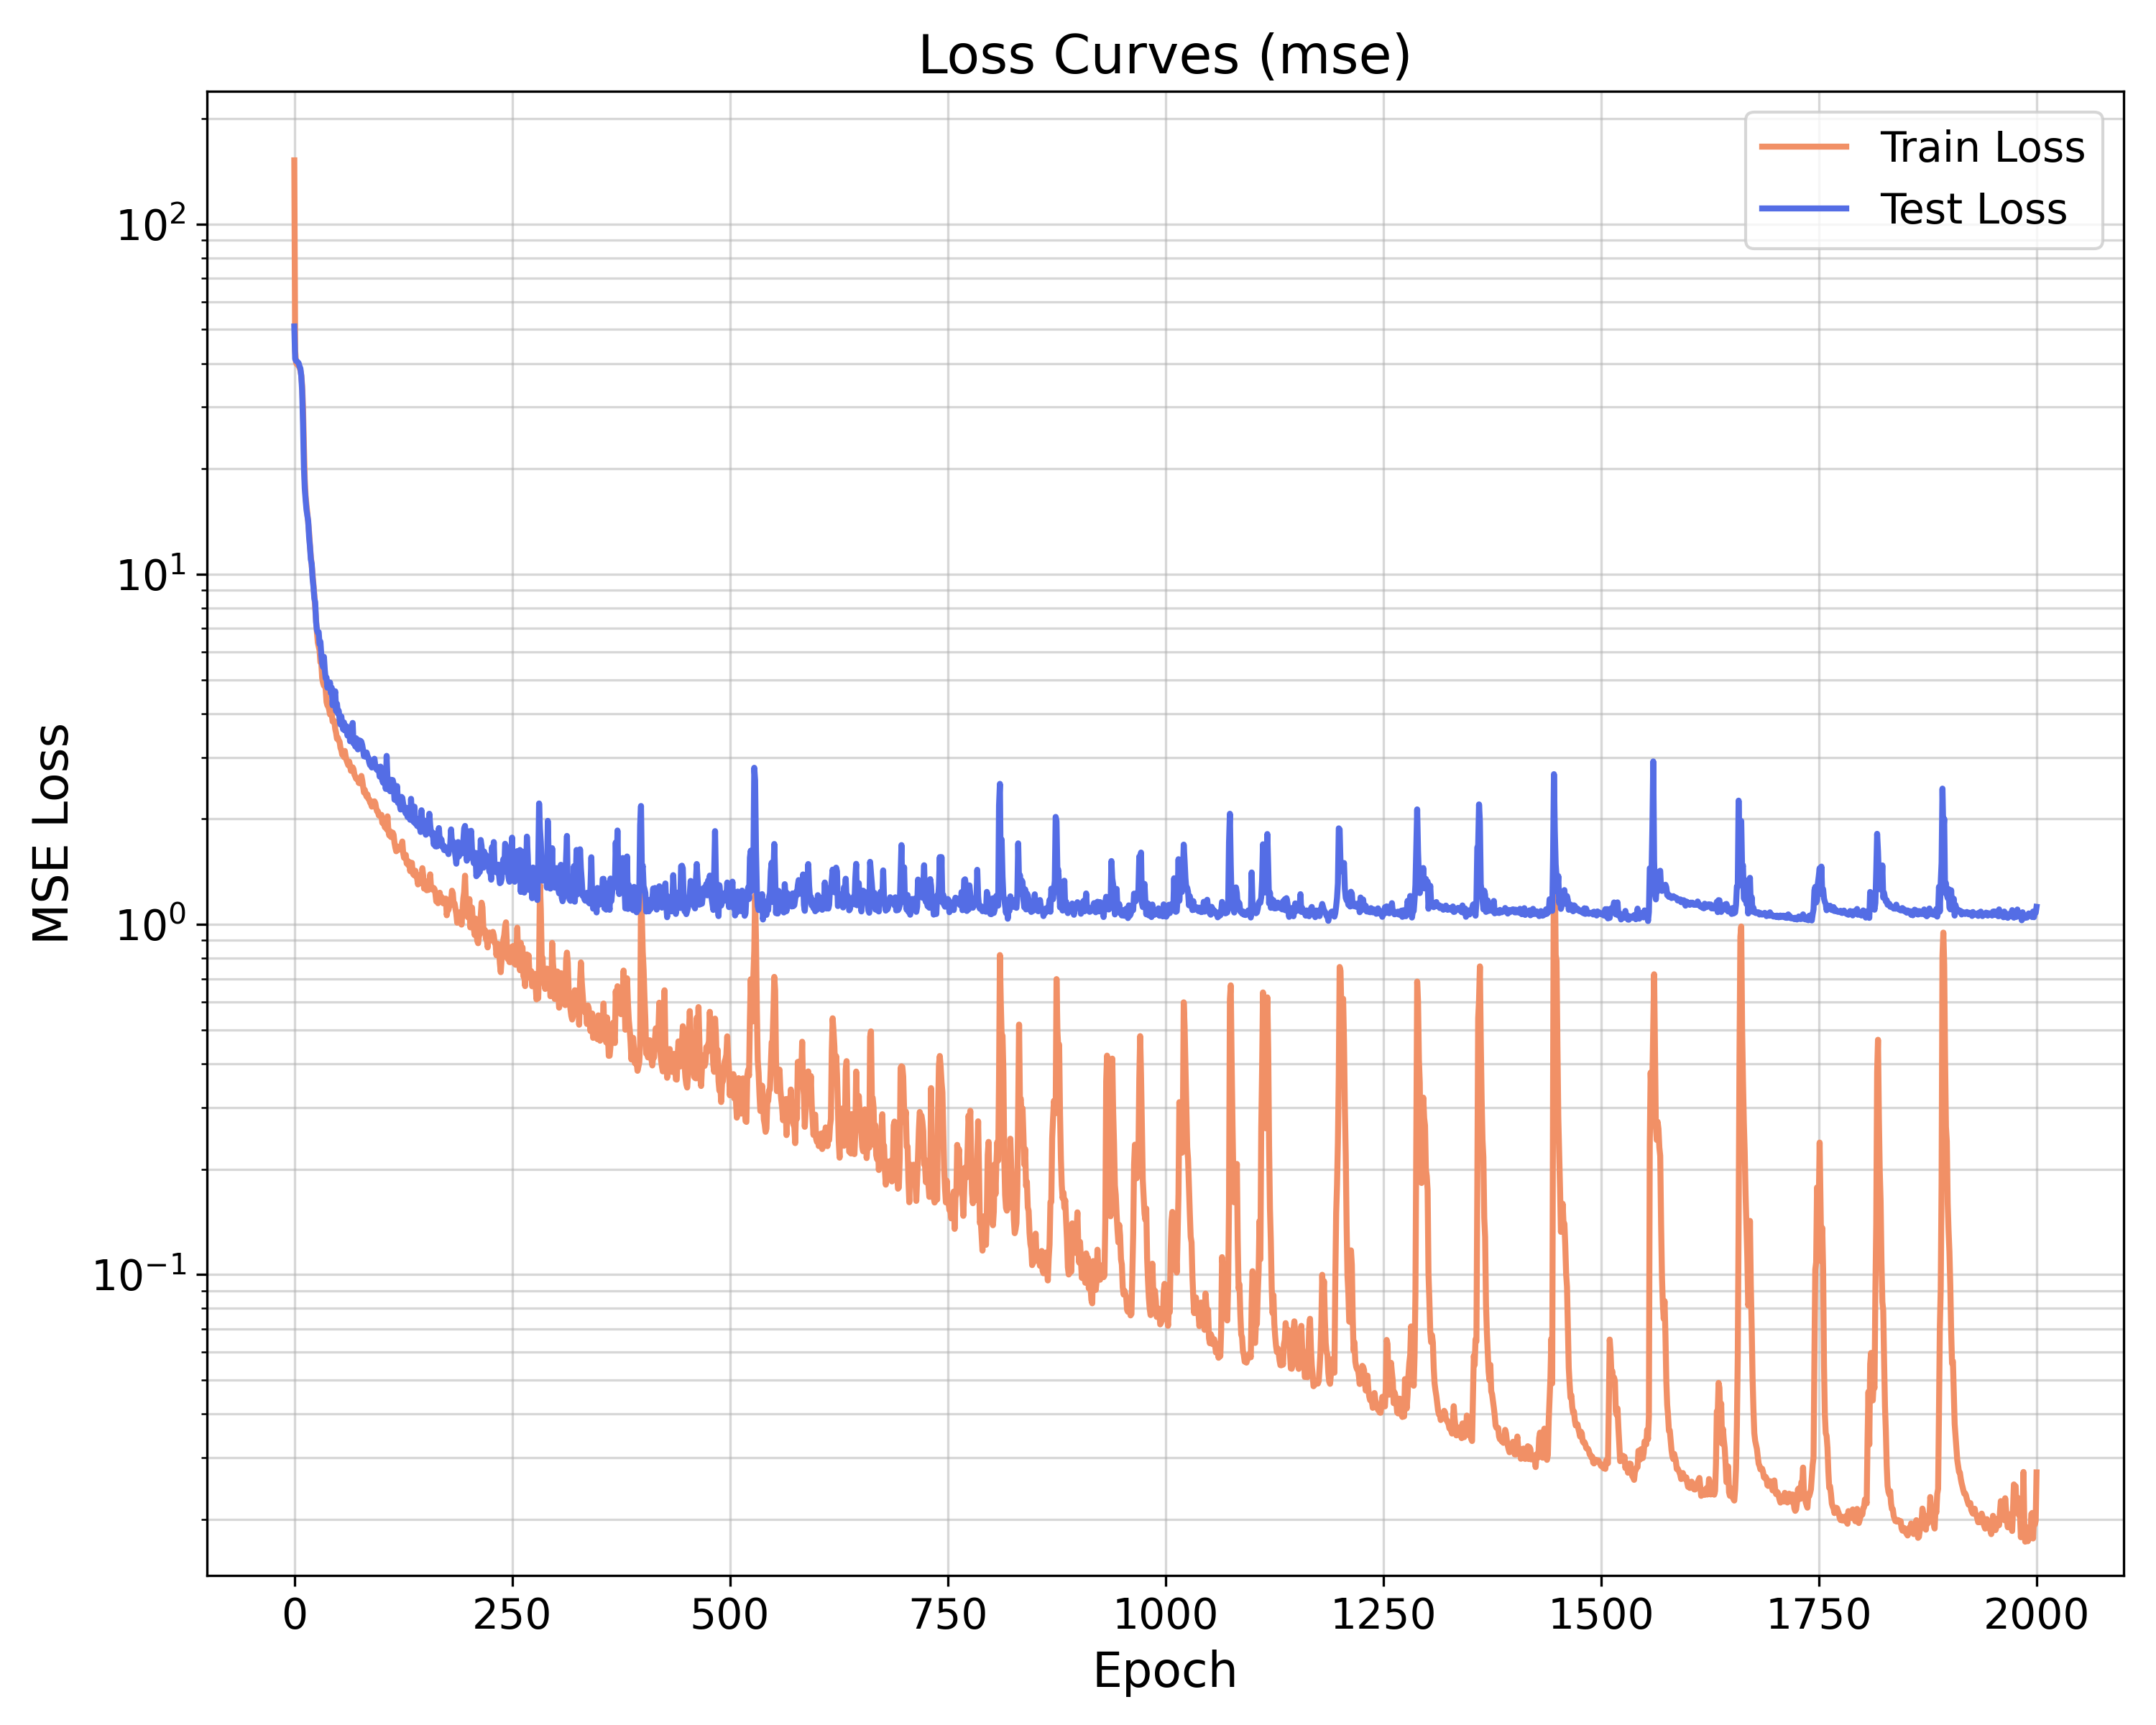
\includegraphics[width=\textwidth]{img/FH_model/ER_Network/FNO/loss_plot_fixed_N=600.png}
        \caption{$N=600$}
    \end{subfigure}
    \hfill
    \begin{subfigure}[b]{0.32\textwidth}
        \centering
        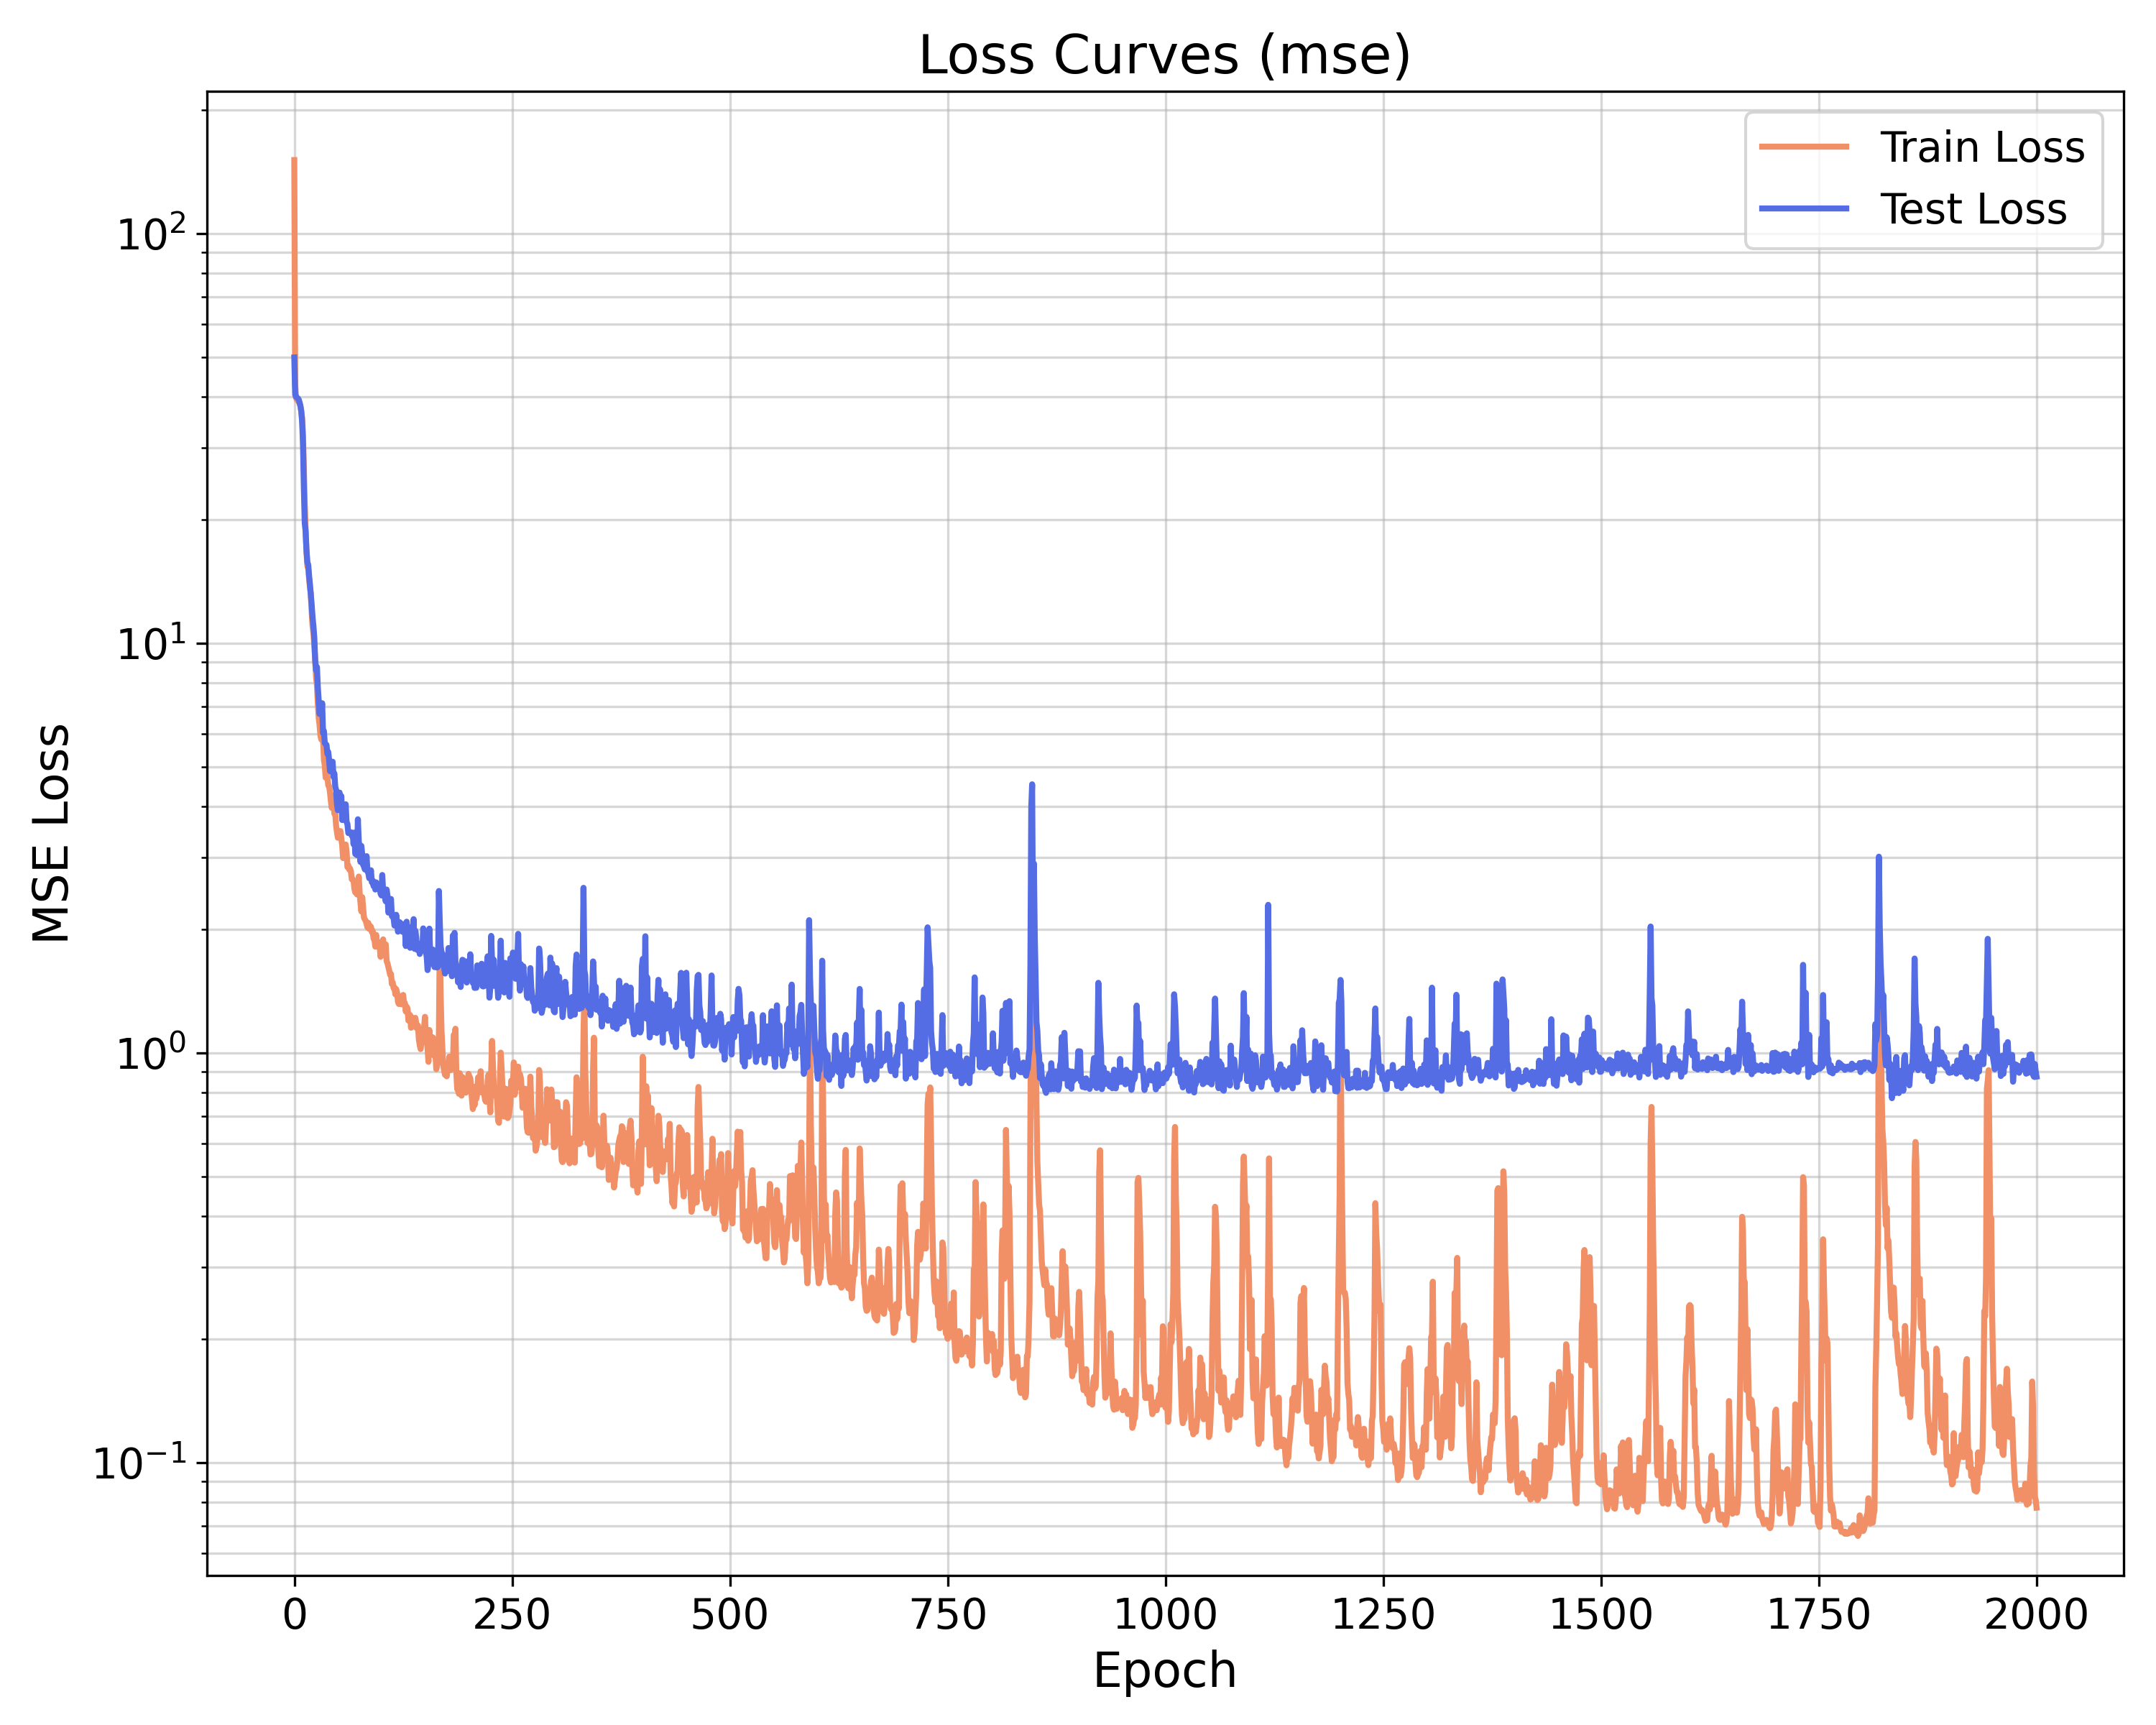
\includegraphics[width=\textwidth]{img/FH_model/ER_Network/FNO/loss_plot_fixed_N=700.png}
        \caption{$N=700$}
    \end{subfigure}
    \hfill
    \begin{subfigure}[b]{0.32\textwidth}
        \centering
        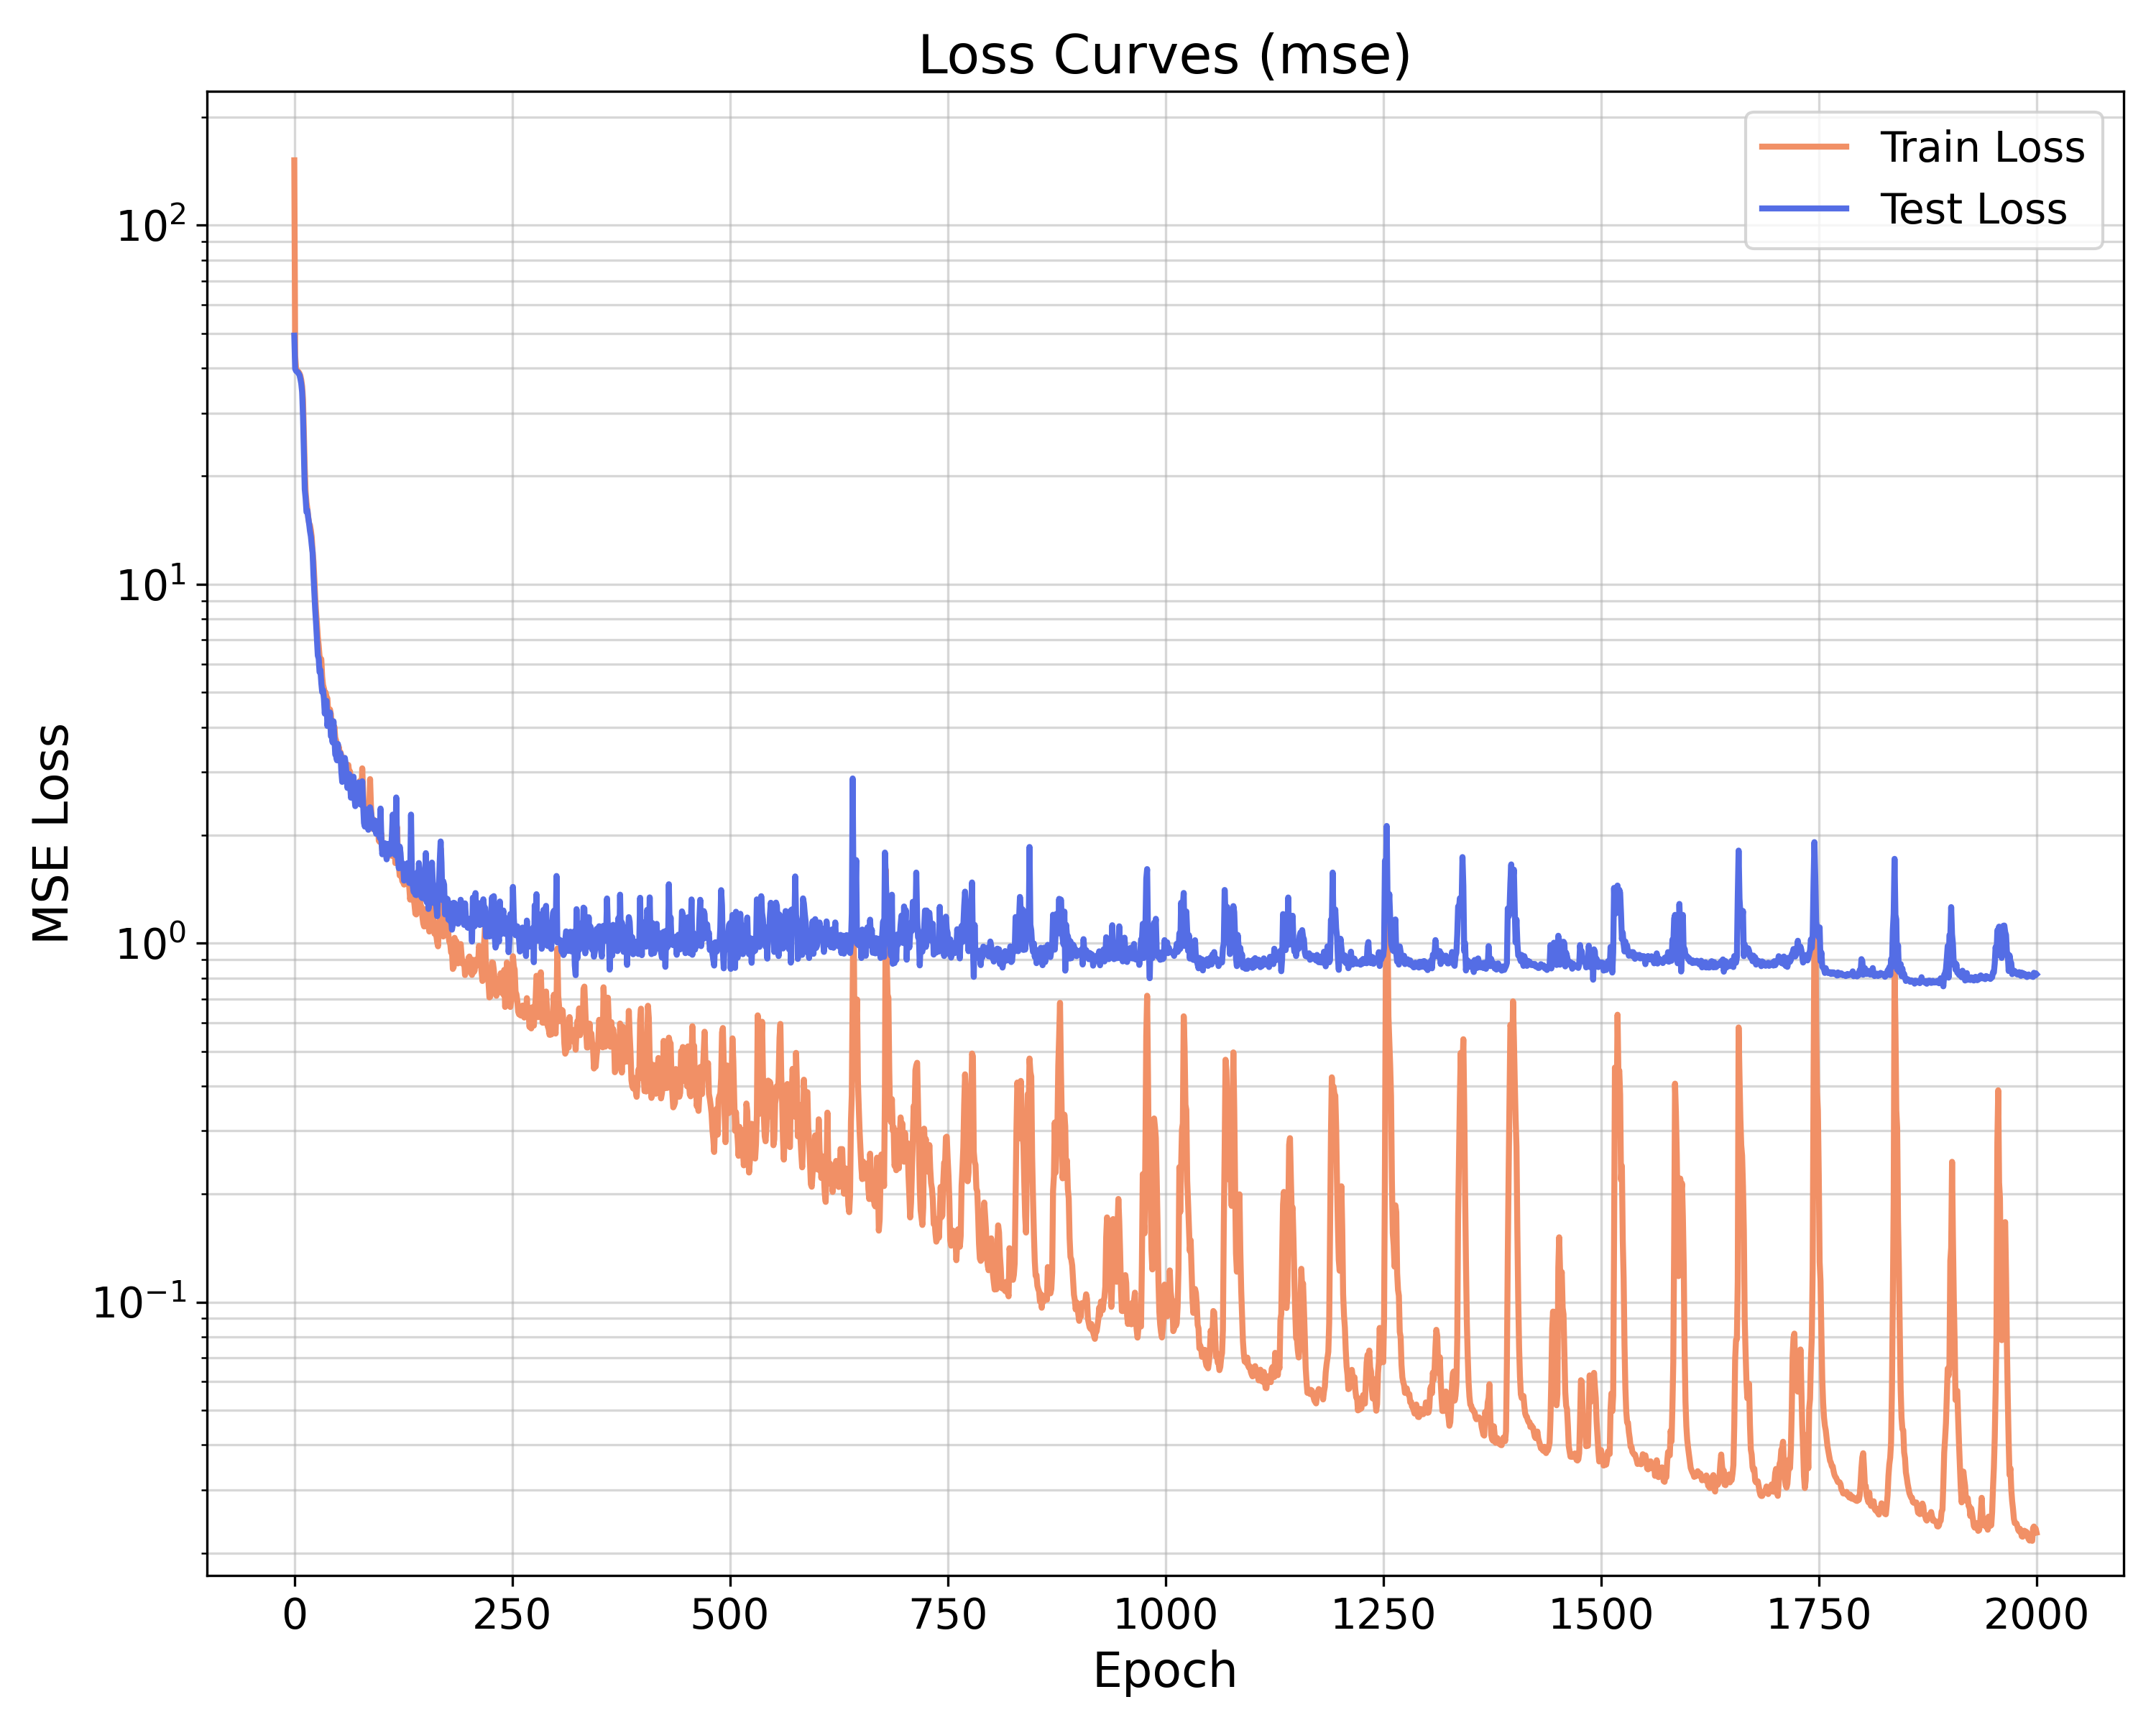
\includegraphics[width=\textwidth]{img/FH_model/ER_Network/FNO/loss_plot_fixed_N=800.png}
        \caption{$N=800$}
    \end{subfigure}
    
    \vspace{0.4cm}
    
    % --- Quarta riga ---
    \begin{subfigure}[b]{0.32\textwidth}
        \centering
        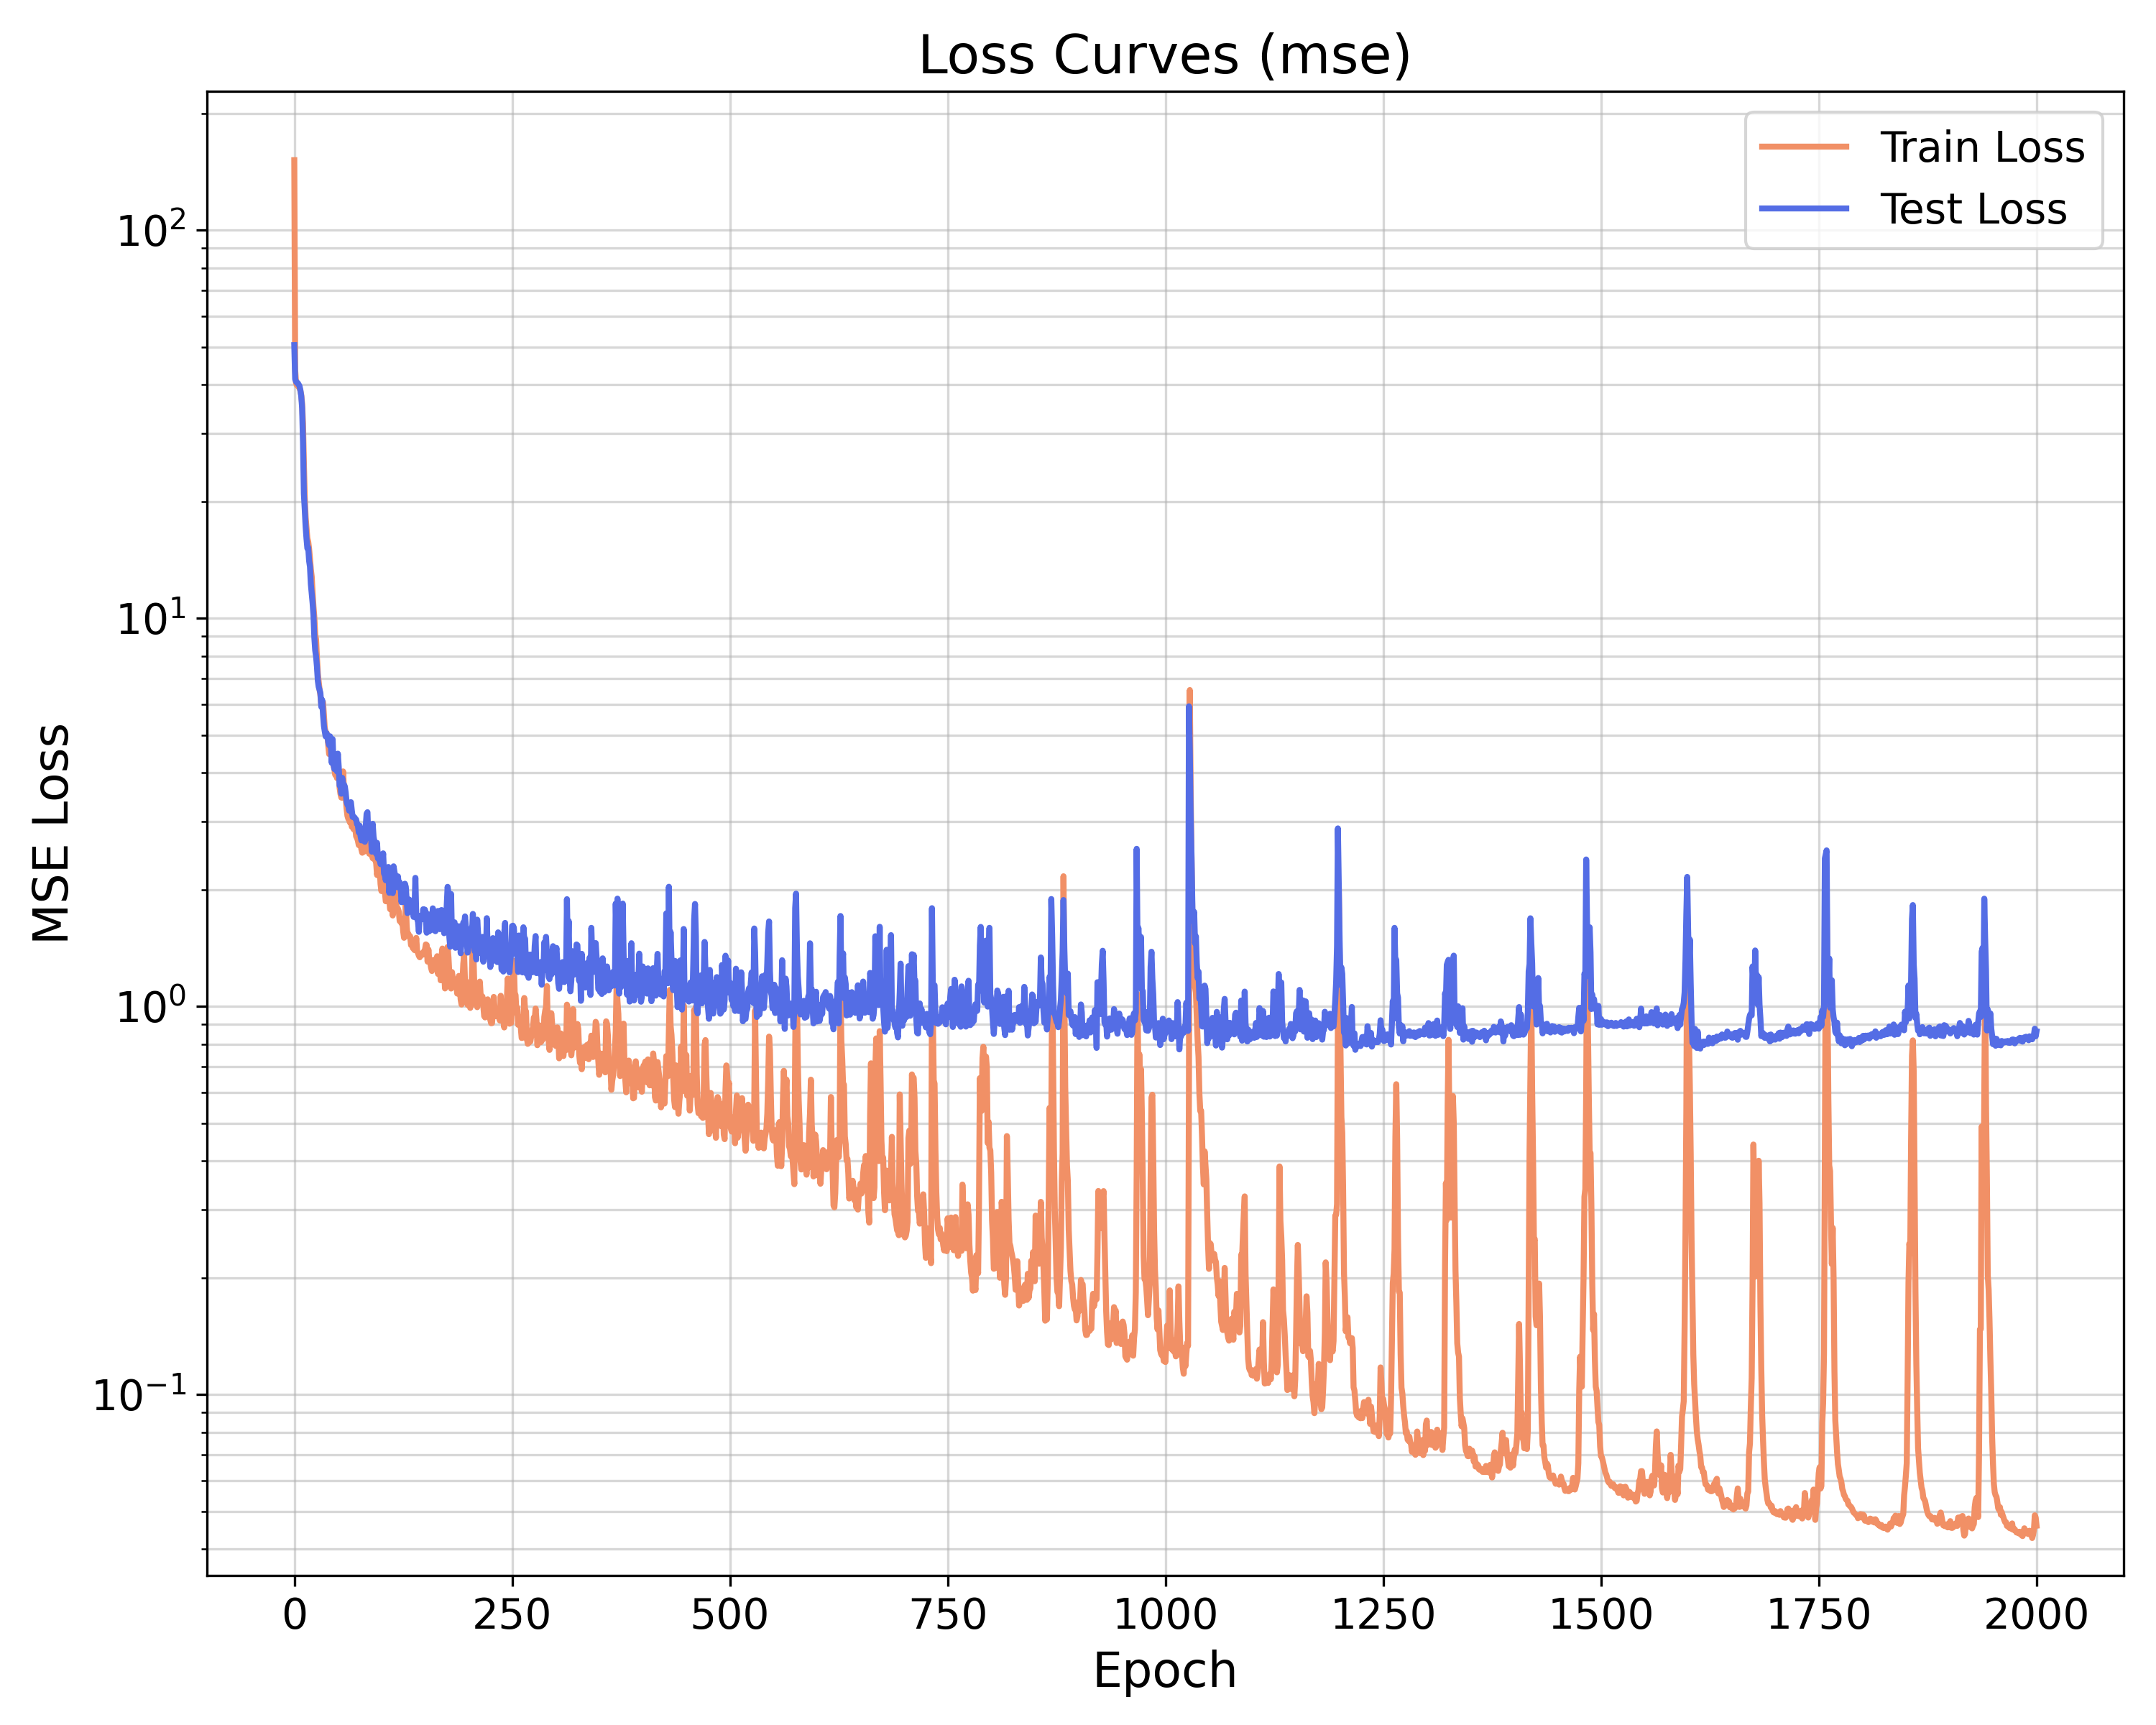
\includegraphics[width=\textwidth]{img/FH_model/ER_Network/FNO/loss_plot_fixed_N=900.png}
        \caption{$N=900$}
    \end{subfigure}
    \hfill
    \begin{subfigure}[b]{0.32\textwidth}
        \centering
        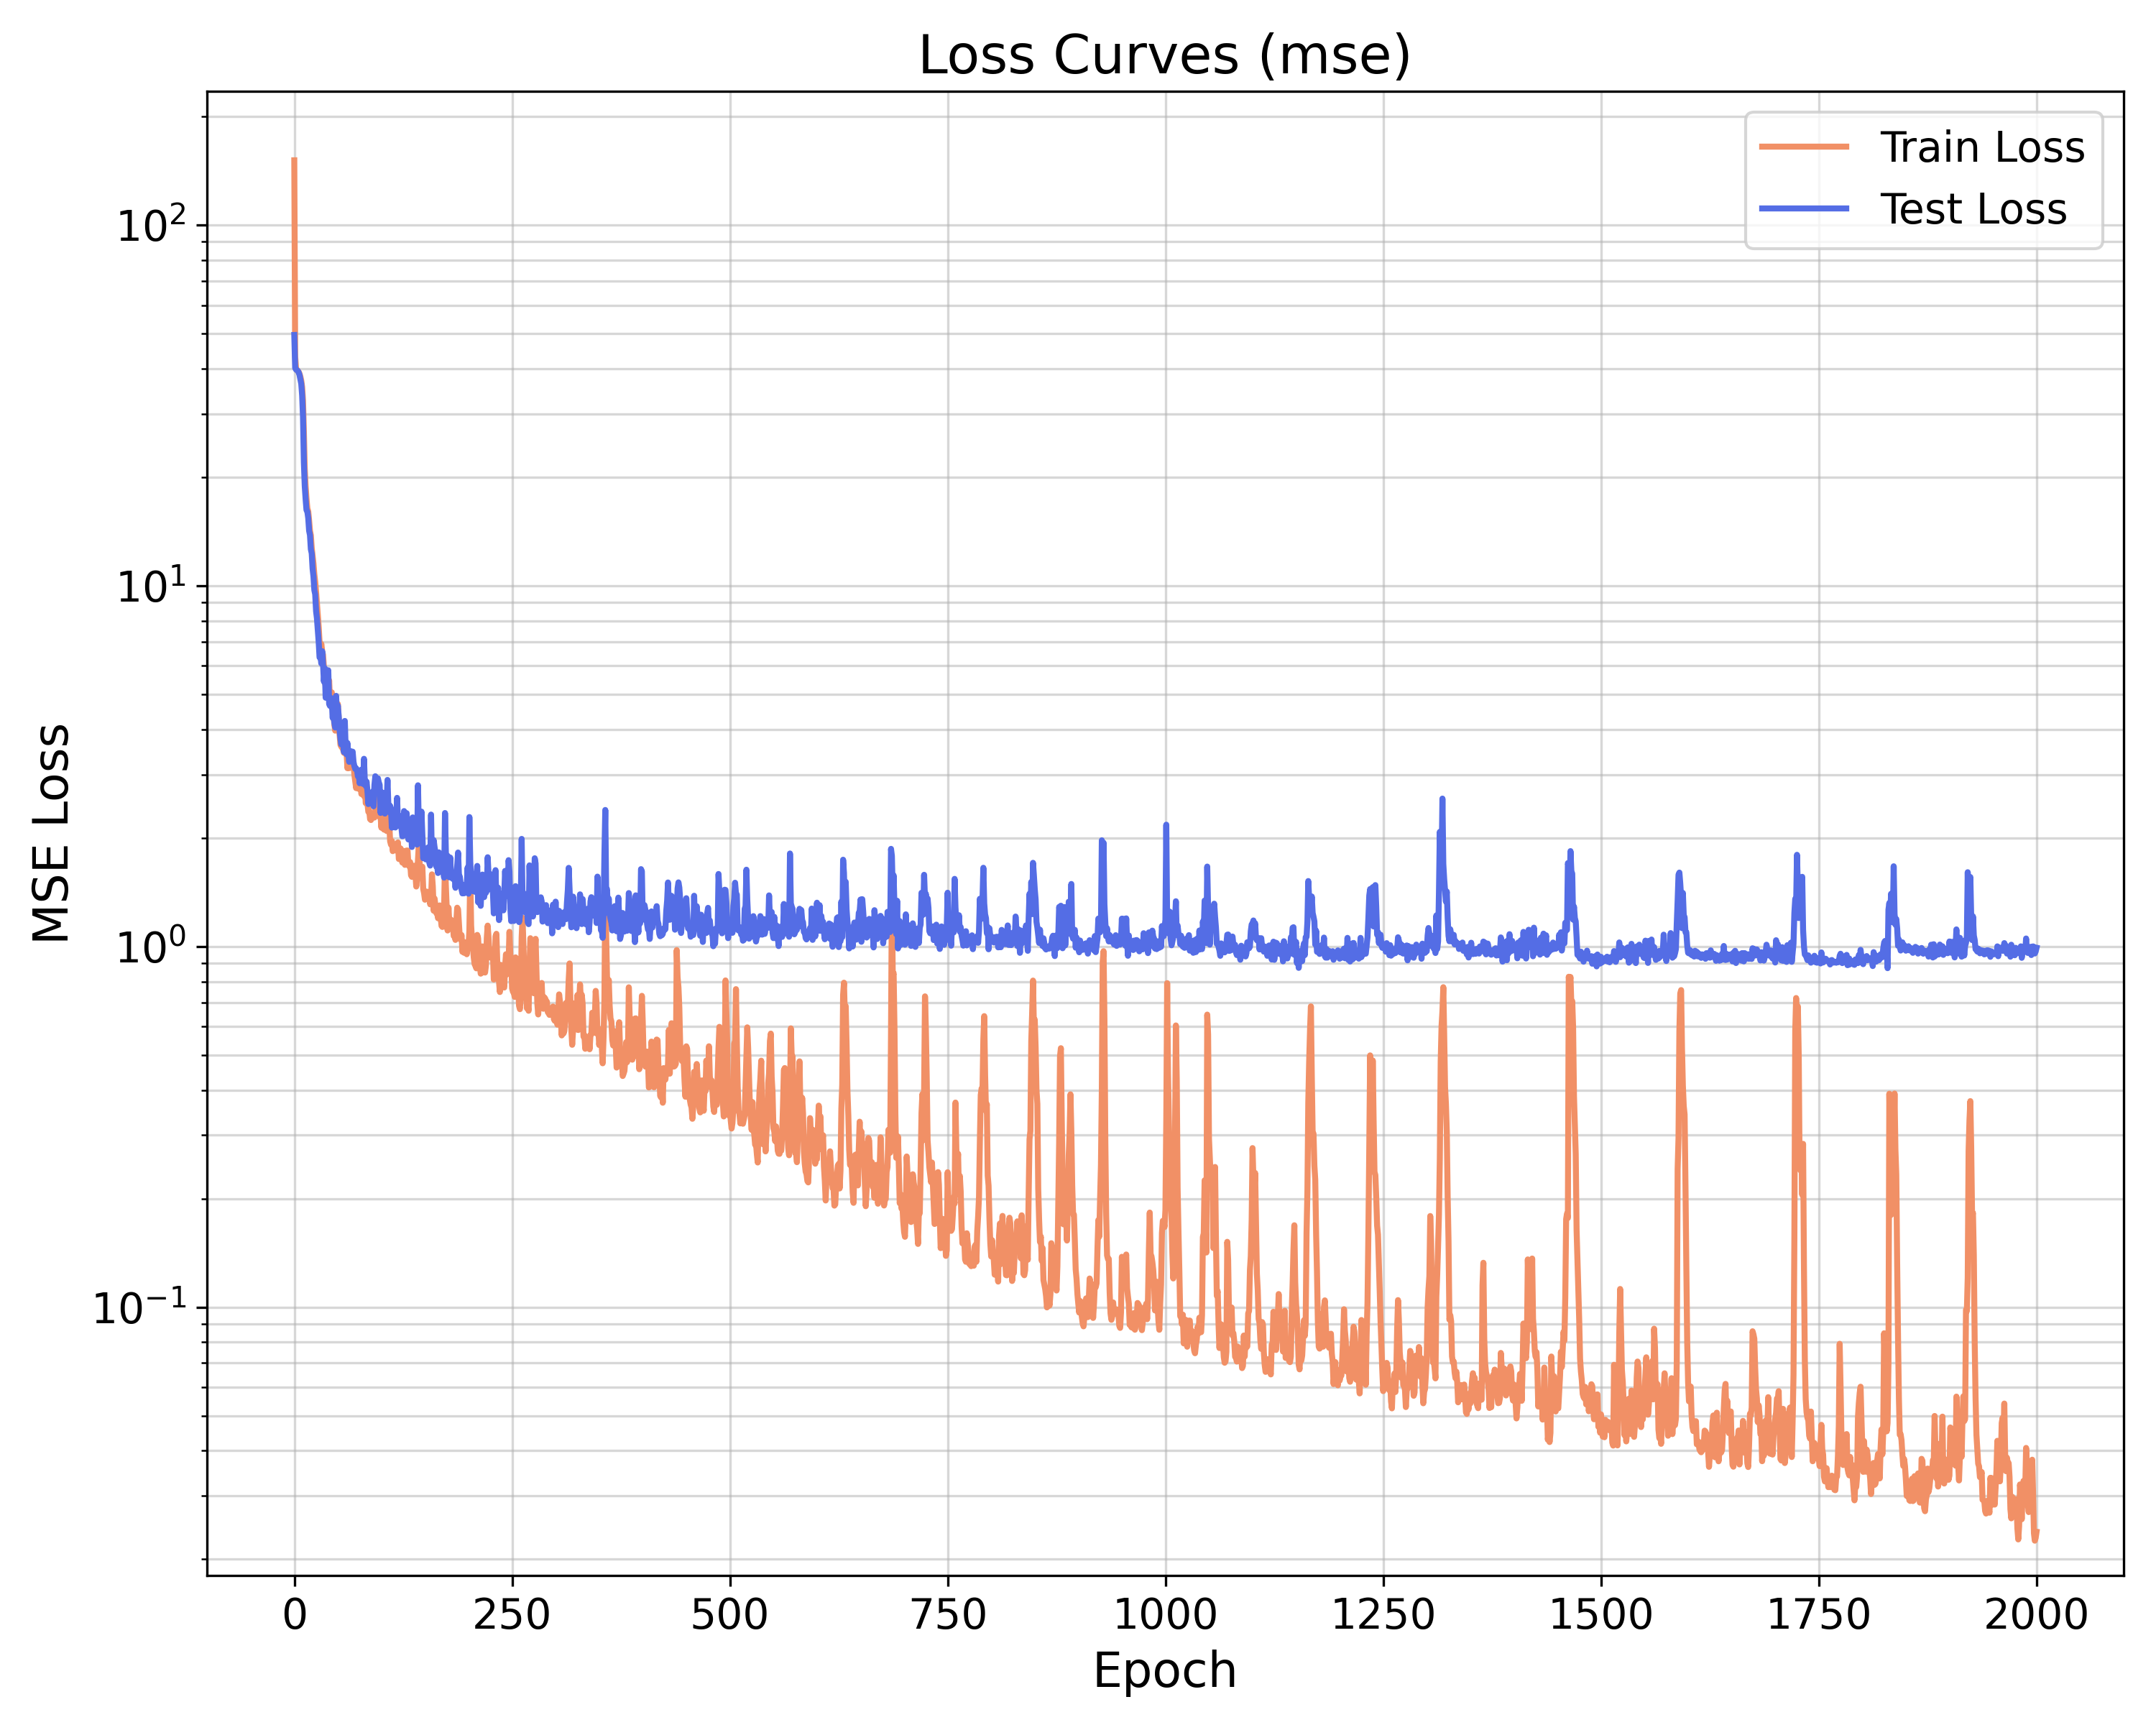
\includegraphics[width=\textwidth]{img/FH_model/ER_Network/FNO/loss_plot_fixed_N=1000.png}
        \caption{$N=1000$}
    \end{subfigure}
    \hfill
    \begin{subfigure}[b]{0.32\textwidth}
        \centering
        
\includegraphics[width=\textwidth]{img/FH_model/ER_Network/FNO/loss_plot_fixed_N=2000.png}
        \caption{$N=2000$}
    \end{subfigure}
    
    \caption{Training and test loss convergence for different Erd\H{o}s-R\'enyi network sizes ($N$).}
    \label{fig:er_loss_grid}
\end{figure}

\subsection{BA network}

Before detailing the results, it is worth briefly recalling that a Barab\'asi-Albert (BA) network is a widely used model for generating random scale-free networks. It relies on a preferential attachment mechanism, meaning that new nodes are more likely to establish connections with existing nodes that already have a high degree.
Due to the particular structure of this family of networks, we defined the hubs as the nodes whose degree exceeds the 95th percentile (representing the top 5\% most connected nodes in the graph). Consequently, we opted to randomly connect the input and output nodes exclusively to one of these hubs.
In this way we greatly reduced the variability of the dynamics due to the seed.

Following the same rationale as the previous section, we proceeded to observe if the performance of FNO degraded with the growing size ($N$) of the hidden network. To conduct this experiment we performed our analysis for different sizes of the BA network: $N= 10,100,200,300,400,500,600,700,800,900,1000,2000$. 
Since the input and output nodes are randomly chosen, we repeated each experiment with different seeds ($0, 42, 100$) to distinguish whether specific effects are intrinsic to the topology or merely due to the chance of the particular sampling of input/output nodes.

Here we reported only figures for the seed $S=42$.

As a representative example of the system's setup, Figure \ref{fig:ba_setup_100} reports the network topology for a BA graph of size $N=100$.

\begin{figure}[htbp]
    \centering
    
\includegraphics[width=\textwidth]{img/FH_model/BA_Network/network_plot_BA_N=100.png}
    \caption{Our setup for a Barab\'asi-Albert network of size $N=100$.}
    \label{fig:ba_setup_100}
\end{figure}


%%%
%%%
% ==========================================
% GRIGLIA 1: PEAKS (Estensione .png)
% ==========================================
\begin{figure}[htbp]
    \centering
    % --- Prima riga ---
    \begin{subfigure}[b]{0.32\textwidth}
        \centering
        
\includegraphics[width=\textwidth]{img/FH_model/BA_Network/FNO/HHpeaks_S=42_N=10.png}
        \caption{$N=10$}
    \end{subfigure}
    \hfill
    \begin{subfigure}[b]{0.32\textwidth}
        \centering
        
\includegraphics[width=\textwidth]{img/FH_model/BA_Network/FNO/HHpeaks_S=42_N=100.png}
        \caption{$N=100$}
    \end{subfigure}
    \hfill
    \begin{subfigure}[b]{0.32\textwidth}
        \centering
        
\includegraphics[width=\textwidth]{img/FH_model/BA_Network/FNO/HHpeaks_S=42_N=200.png}
        \caption{$N=200$}
    \end{subfigure}
    
    \vspace{0.4cm}
    
    % --- Seconda riga ---
    \begin{subfigure}[b]{0.32\textwidth}
        \centering
        
\includegraphics[width=\textwidth]{img/FH_model/BA_Network/FNO/HHpeaks_S=42_N=300.png}
        \caption{$N=300$}
    \end{subfigure}
    \hfill
    \begin{subfigure}[b]{0.32\textwidth}
        \centering
        
\includegraphics[width=\textwidth]{img/FH_model/BA_Network/FNO/HHpeaks_S=42_N=400.png}
        \caption{$N=400$}
    \end{subfigure}
    \hfill
    \begin{subfigure}[b]{0.32\textwidth}
        \centering
        
\includegraphics[width=\textwidth]{img/FH_model/BA_Network/FNO/HHpeaks_S=42_N=500.png}
        \caption{$N=500$}
    \end{subfigure}
    
    \vspace{0.4cm}
    
    % --- Terza riga ---
    \begin{subfigure}[b]{0.32\textwidth}
        \centering
        
\includegraphics[width=\textwidth]{img/FH_model/BA_Network/FNO/HHpeaks_S=42_N=600.png}
        \caption{$N=600$}
    \end{subfigure}
    \hfill
    \begin{subfigure}[b]{0.32\textwidth}
        \centering
        
\includegraphics[width=\textwidth]{img/FH_model/BA_Network/FNO/HHpeaks_S=42_N=700.png}
        \caption{$N=700$}
    \end{subfigure}
    \hfill
    \begin{subfigure}[b]{0.32\textwidth}
        \centering
        
\includegraphics[width=\textwidth]{img/FH_model/BA_Network/FNO/HHpeaks_S=42_N=800.png}
        \caption{$N=800$}
    \end{subfigure}
    
    \vspace{0.4cm}
    
    % --- Quarta riga ---
    \begin{subfigure}[b]{0.32\textwidth}
        \centering
        
\includegraphics[width=\textwidth]{img/FH_model/BA_Network/FNO/HHpeaks_S=42_N=900.png}
        \caption{$N=900$}
    \end{subfigure}
    \hfill
    \begin{subfigure}[b]{0.32\textwidth}
        \centering
        
\includegraphics[width=\textwidth]{img/FH_model/BA_Network/FNO/HHpeaks_S=42_N=1000.png}
        \caption{$N=1000$}
    \end{subfigure}
    \hfill
    \begin{subfigure}[b]{0.32\textwidth}
        \centering
        
\includegraphics[width=\textwidth]{img/FH_model/BA_Network/FNO/HHpeaks_S=42_N=2000.png}
        \caption{$N=2000$}
    \end{subfigure}
    
    \caption{Some instances of the test set for different Barab\'asi-Albert network sizes ($N$). For each column we can see the applied input current (bottom) with its corresponding potential response (top): the blue line represents the result of the simulations, whereas the dotted red line indicates the output of the NN.}
    \label{fig:ba_peaks_grid}
\end{figure}

%%%
% ==========================================
% GRIGLIA 2: MSE HISTOGRAMS (Estensione .png)
% ==========================================

\begin{figure}[htbp]
    \centering
    % --- Prima riga ---
    \begin{subfigure}[b]{0.32\textwidth}
        \centering
        
\includegraphics[width=\textwidth]{img/FH_model/BA_Network/FNO/L2histoFNO_S=42_N=10.png}
        \caption{$N=10$}
    \end{subfigure}
    \hfill
    \begin{subfigure}[b]{0.32\textwidth}
        \centering
        
\includegraphics[width=\textwidth]{img/FH_model/BA_Network/FNO/L2histoFNO_S=42_N=100.png}
        \caption{$N=100$}
    \end{subfigure}
    \hfill
    \begin{subfigure}[b]{0.32\textwidth}
        \centering
        
\includegraphics[width=\textwidth]{img/FH_model/BA_Network/FNO/L2histoFNO_S=42_N=200.png}
        \caption{$N=200$}
    \end{subfigure}
    
    \vspace{0.4cm}
    
    % --- Seconda riga ---
    \begin{subfigure}[b]{0.32\textwidth}
        \centering
        
\includegraphics[width=\textwidth]{img/FH_model/BA_Network/FNO/L2histoFNO_S=42_N=300.png}
        \caption{$N=300$}
    \end{subfigure}
    \hfill
    \begin{subfigure}[b]{0.32\textwidth}
        \centering
        
\includegraphics[width=\textwidth]{img/FH_model/BA_Network/FNO/L2histoFNO_S=42_N=400.png}
        \caption{$N=400$}
    \end{subfigure}
    \hfill
    \begin{subfigure}[b]{0.32\textwidth}
        \centering
        
\includegraphics[width=\textwidth]{img/FH_model/BA_Network/FNO/L2histoFNO_S=42_N=500.png}
        \caption{$N=500$}
    \end{subfigure}
    
    \vspace{0.4cm}
    
    % --- Terza riga ---
    \begin{subfigure}[b]{0.32\textwidth}
        \centering
        
\includegraphics[width=\textwidth]{img/FH_model/BA_Network/FNO/L2histoFNO_S=42_N=600.png}
        \caption{$N=600$}
    \end{subfigure}
    \hfill
    \begin{subfigure}[b]{0.32\textwidth}
        \centering
        
\includegraphics[width=\textwidth]{img/FH_model/BA_Network/FNO/L2histoFNO_S=42_N=700.png}
        \caption{$N=700$}
    \end{subfigure}
    \hfill
    \begin{subfigure}[b]{0.32\textwidth}
        \centering
        
\includegraphics[width=\textwidth]{img/FH_model/BA_Network/FNO/L2histoFNO_S=42_N=800.png}
        \caption{$N=800$}
    \end{subfigure}
    
    \vspace{0.4cm}
    
    % --- Quarta riga ---
    \begin{subfigure}[b]{0.32\textwidth}
        \centering
        
\includegraphics[width=\textwidth]{img/FH_model/BA_Network/FNO/L2histoFNO_S=42_N=900.png}
        \caption{$N=900$}
    \end{subfigure}
    \hfill
    \begin{subfigure}[b]{0.32\textwidth}
        \centering
        
\includegraphics[width=\textwidth]{img/FH_model/BA_Network/FNO/L2histoFNO_S=42_N=1000.png}
        \caption{$N=1000$}
    \end{subfigure}
    \hfill
    \begin{subfigure}[b]{0.32\textwidth}
        \centering
        
\includegraphics[width=\textwidth]{img/FH_model/BA_Network/FNO/L2histoFNO_S=42_N=2000.png}
        \caption{$N=2000$}
    \end{subfigure}
    
    \caption{MSE error distributions across the test set for different Barab\'asi-Albert network sizes ($N$).}
    \label{fig:ba_histo_grid}
\end{figure}

% ==========================================
% GRIGLIA 3: LOSS PLOTS (Estensione .png)
% ==========================================
\begin{figure}[htbp]
    \centering
    % --- Prima riga ---
    \begin{subfigure}[b]{0.32\textwidth}
        \centering
        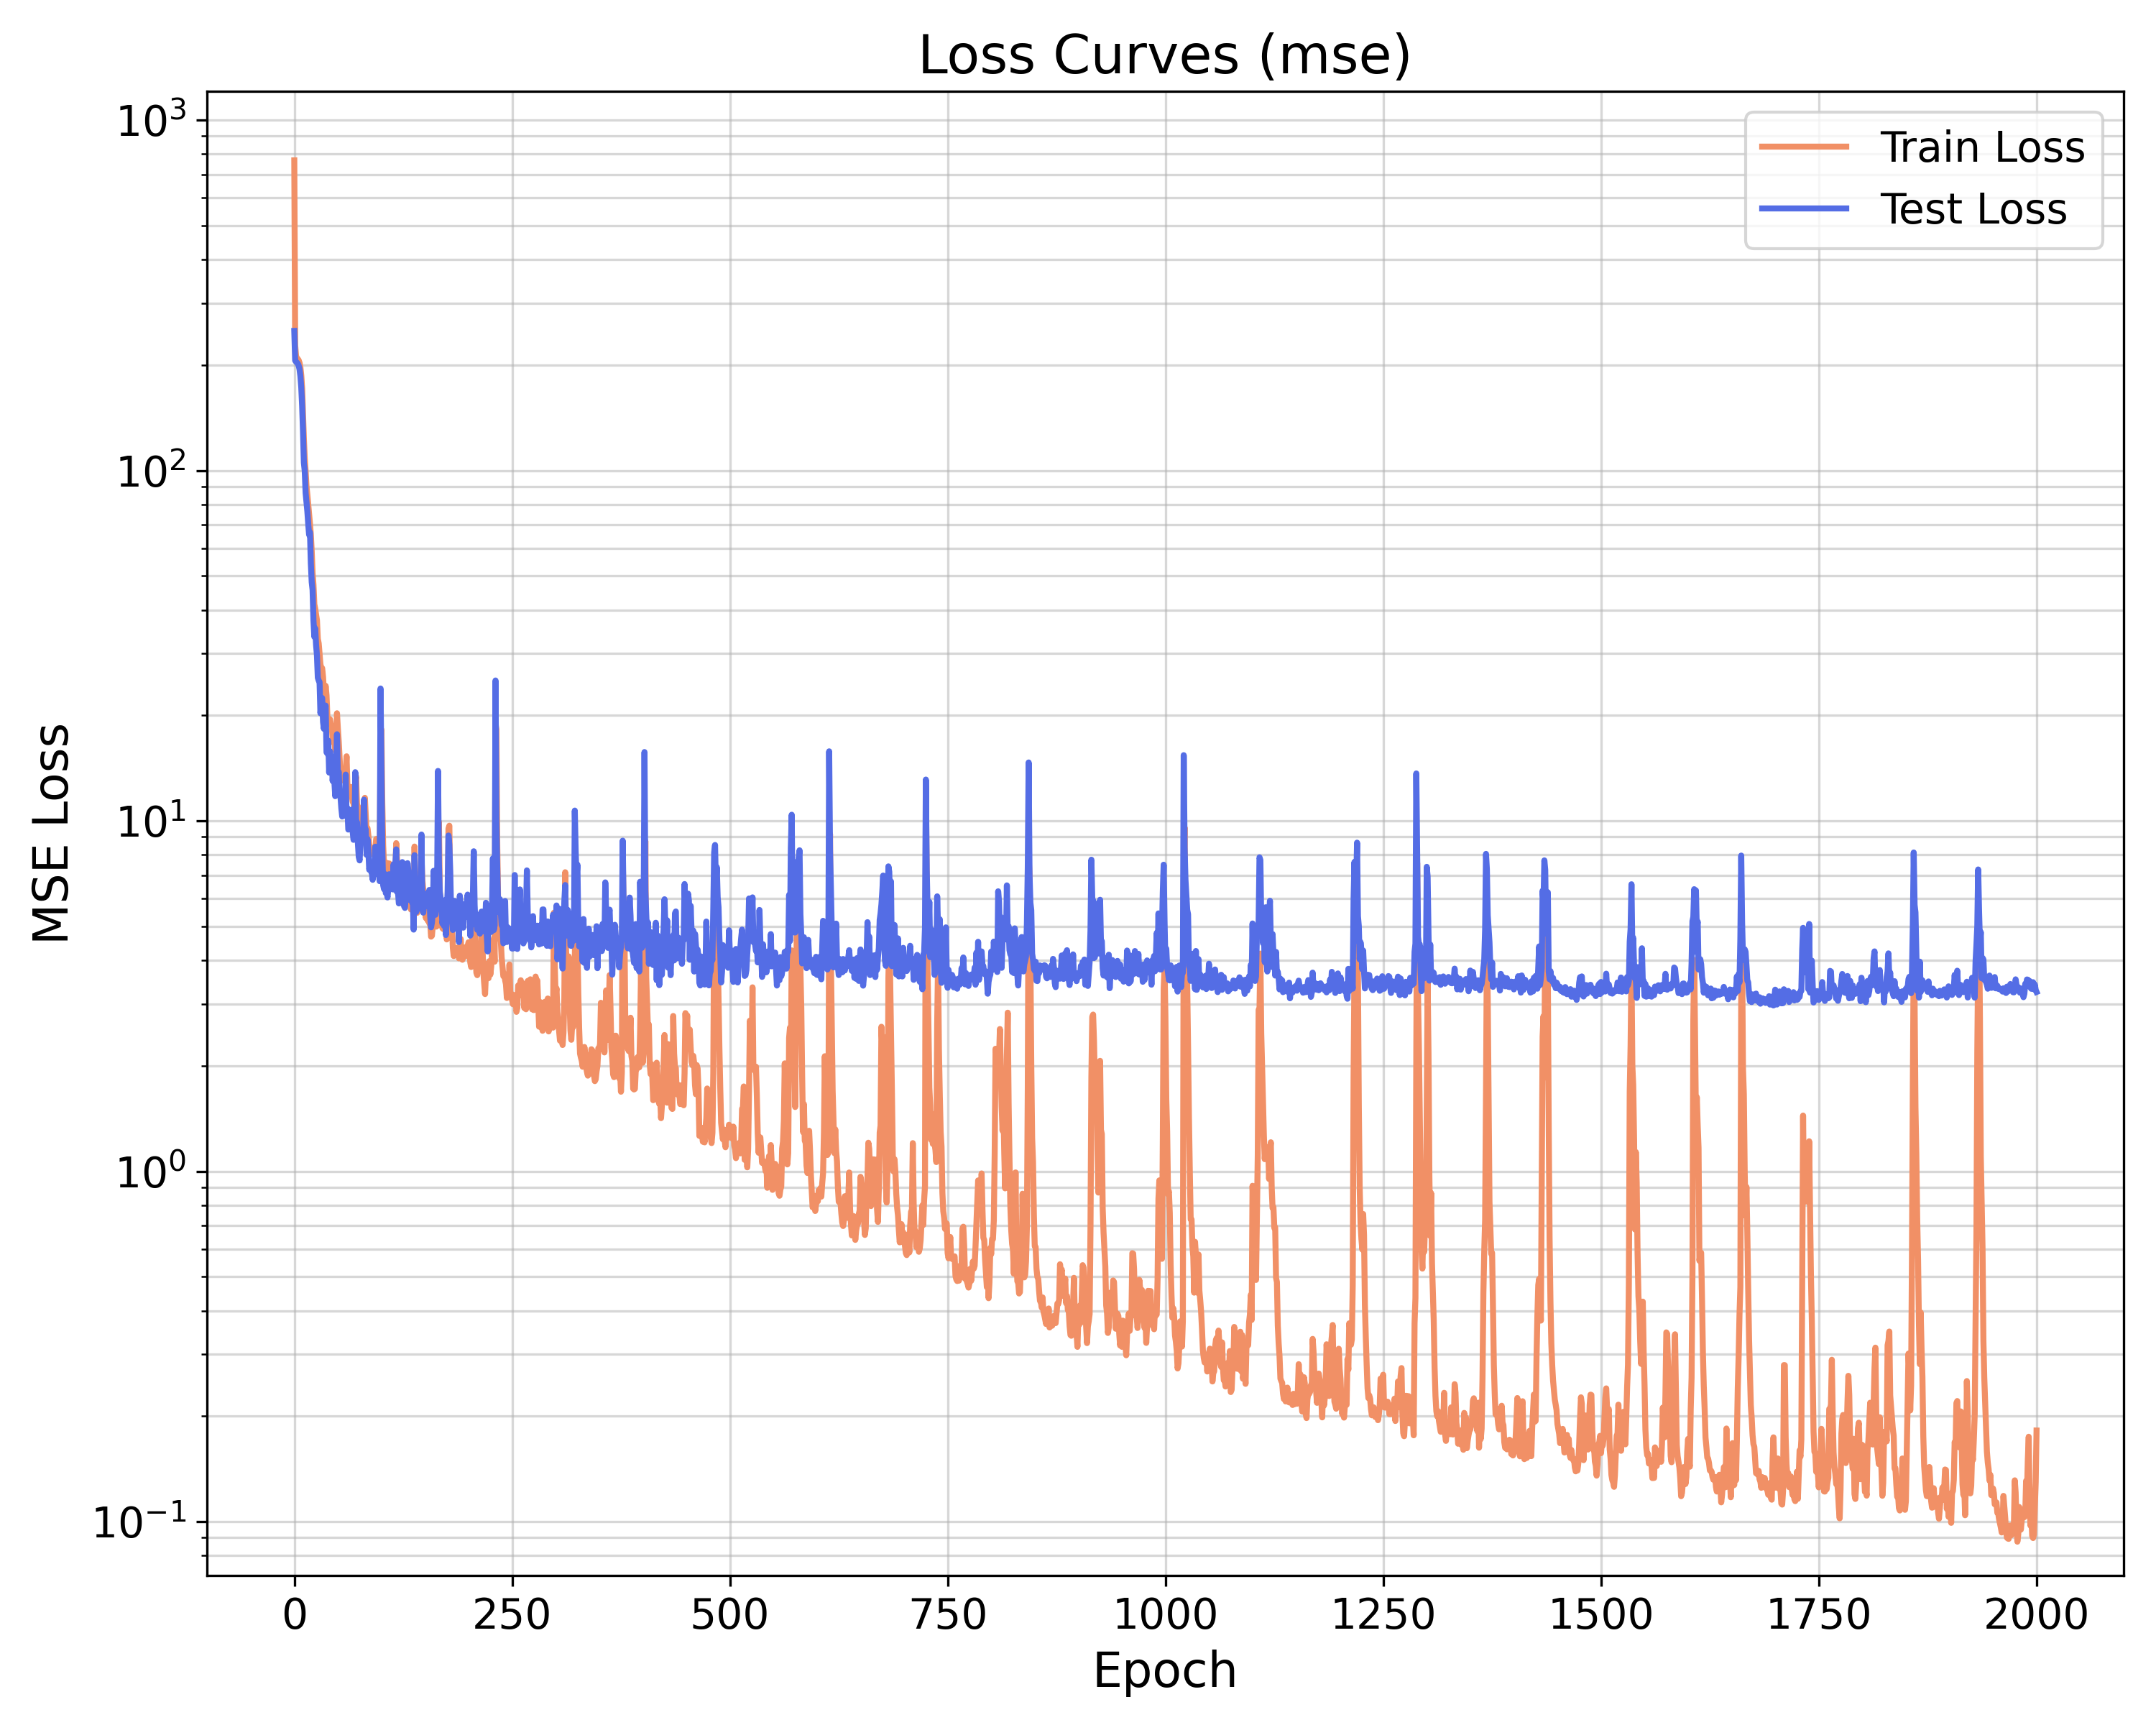
\includegraphics[width=\textwidth]{img/FH_model/BA_Network/FNO/loss_plot_fixed_S=42_N=10.png}
        \caption{$N=10$}
    \end{subfigure}
    \hfill
    \begin{subfigure}[b]{0.32\textwidth}
        \centering
        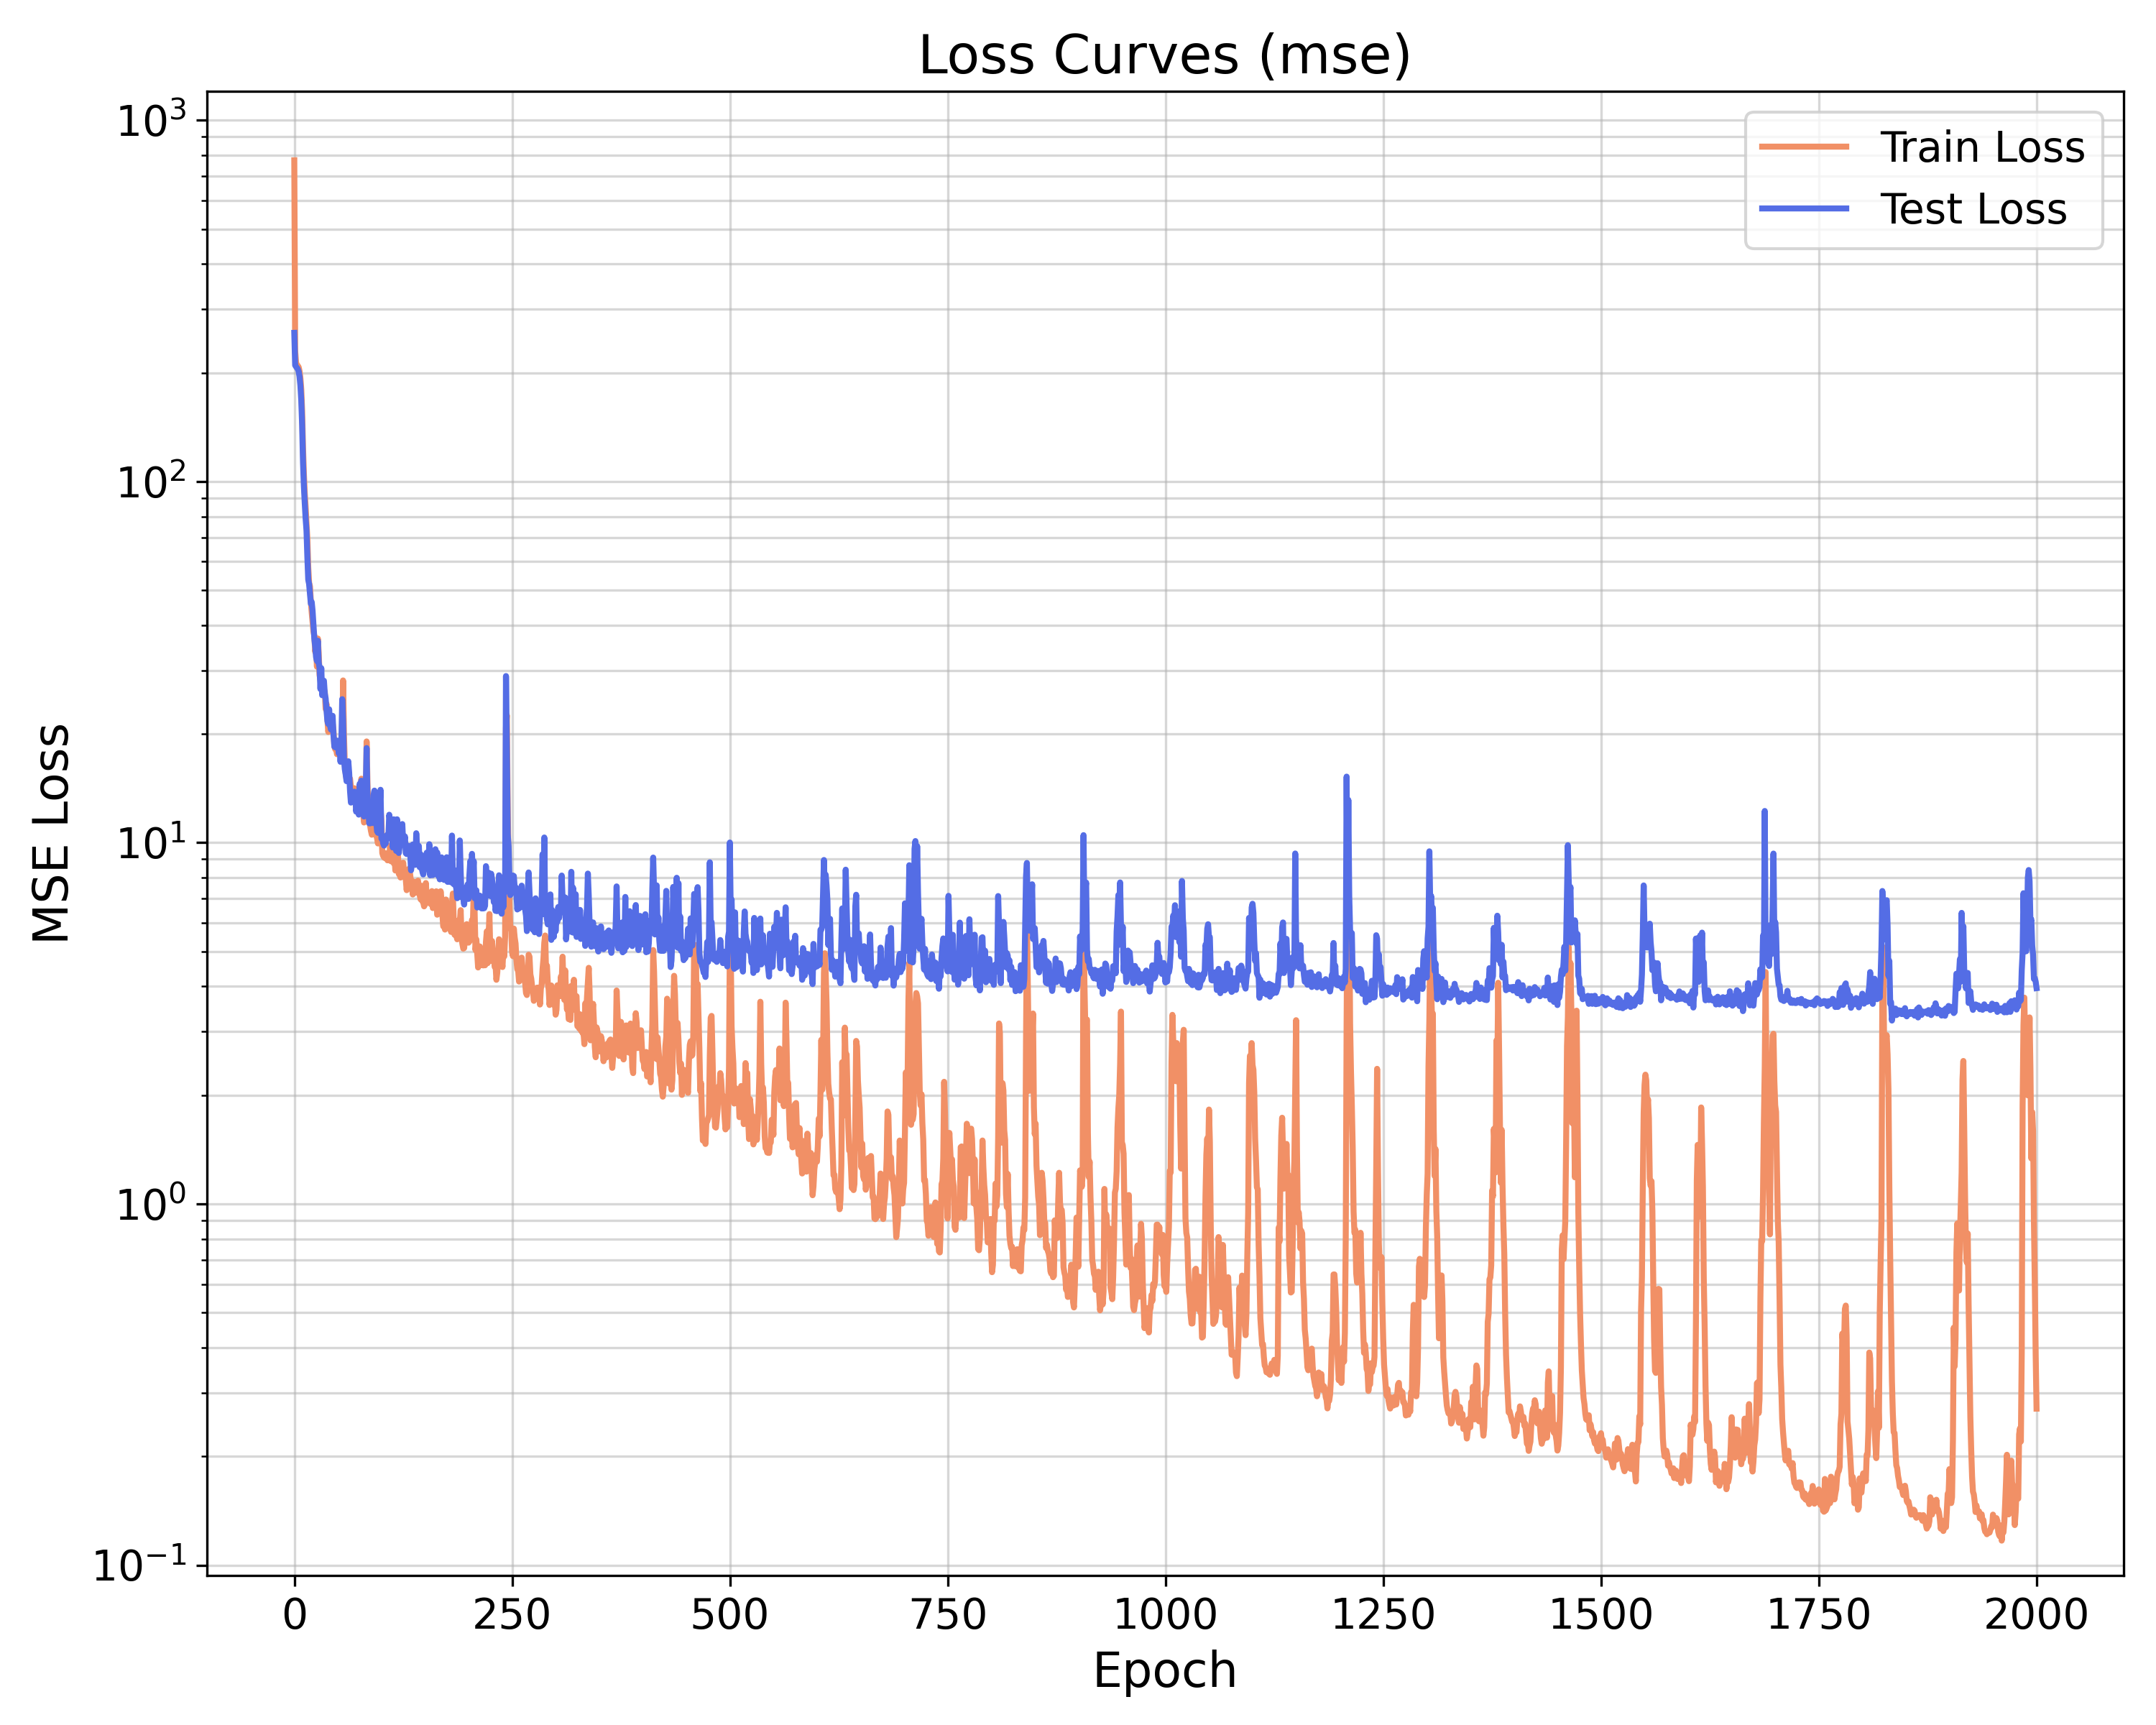
\includegraphics[width=\textwidth]{img/FH_model/BA_Network/FNO/loss_plot_fixed_S=42_N=100.png}
        \caption{$N=100$}
    \end{subfigure}
    \hfill
    \begin{subfigure}[b]{0.32\textwidth}
        \centering
        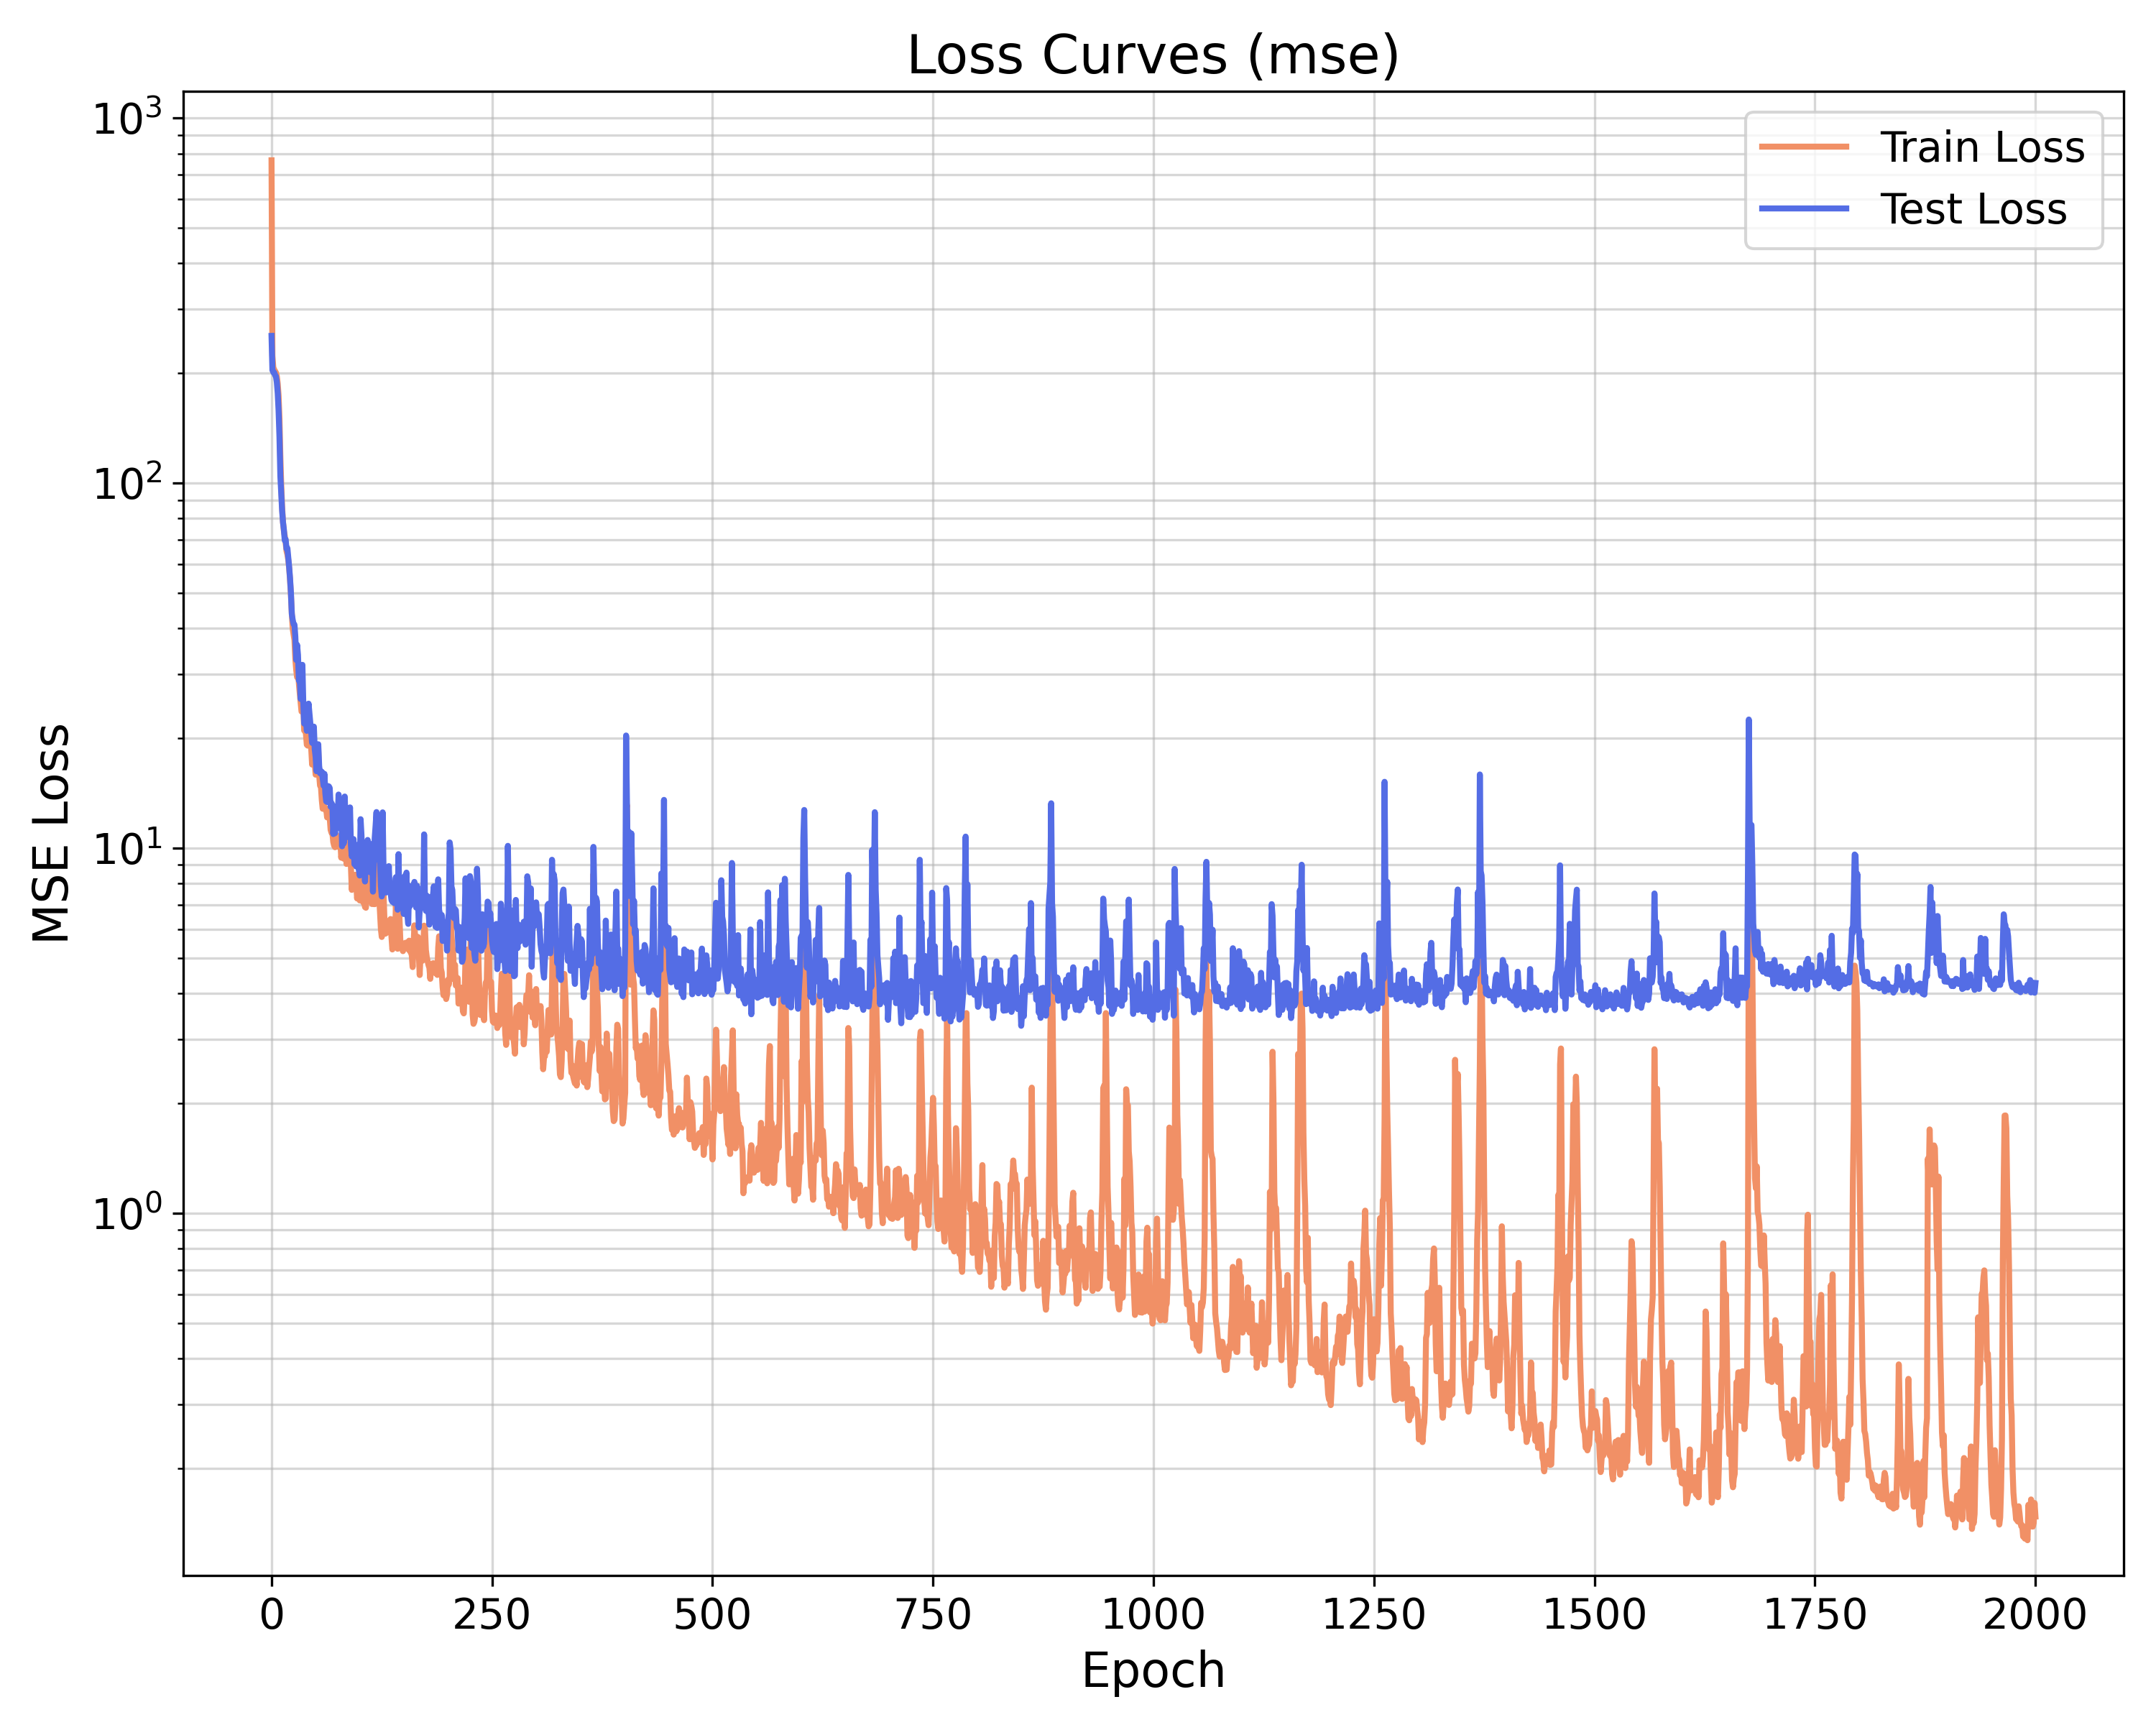
\includegraphics[width=\textwidth]{img/FH_model/BA_Network/FNO/loss_plot_fixed_S=42_N=200.png}
        \caption{$N=200$}
    \end{subfigure}
    
    \vspace{0.4cm}
    
    % --- Seconda riga ---
    \begin{subfigure}[b]{0.32\textwidth}
        \centering
        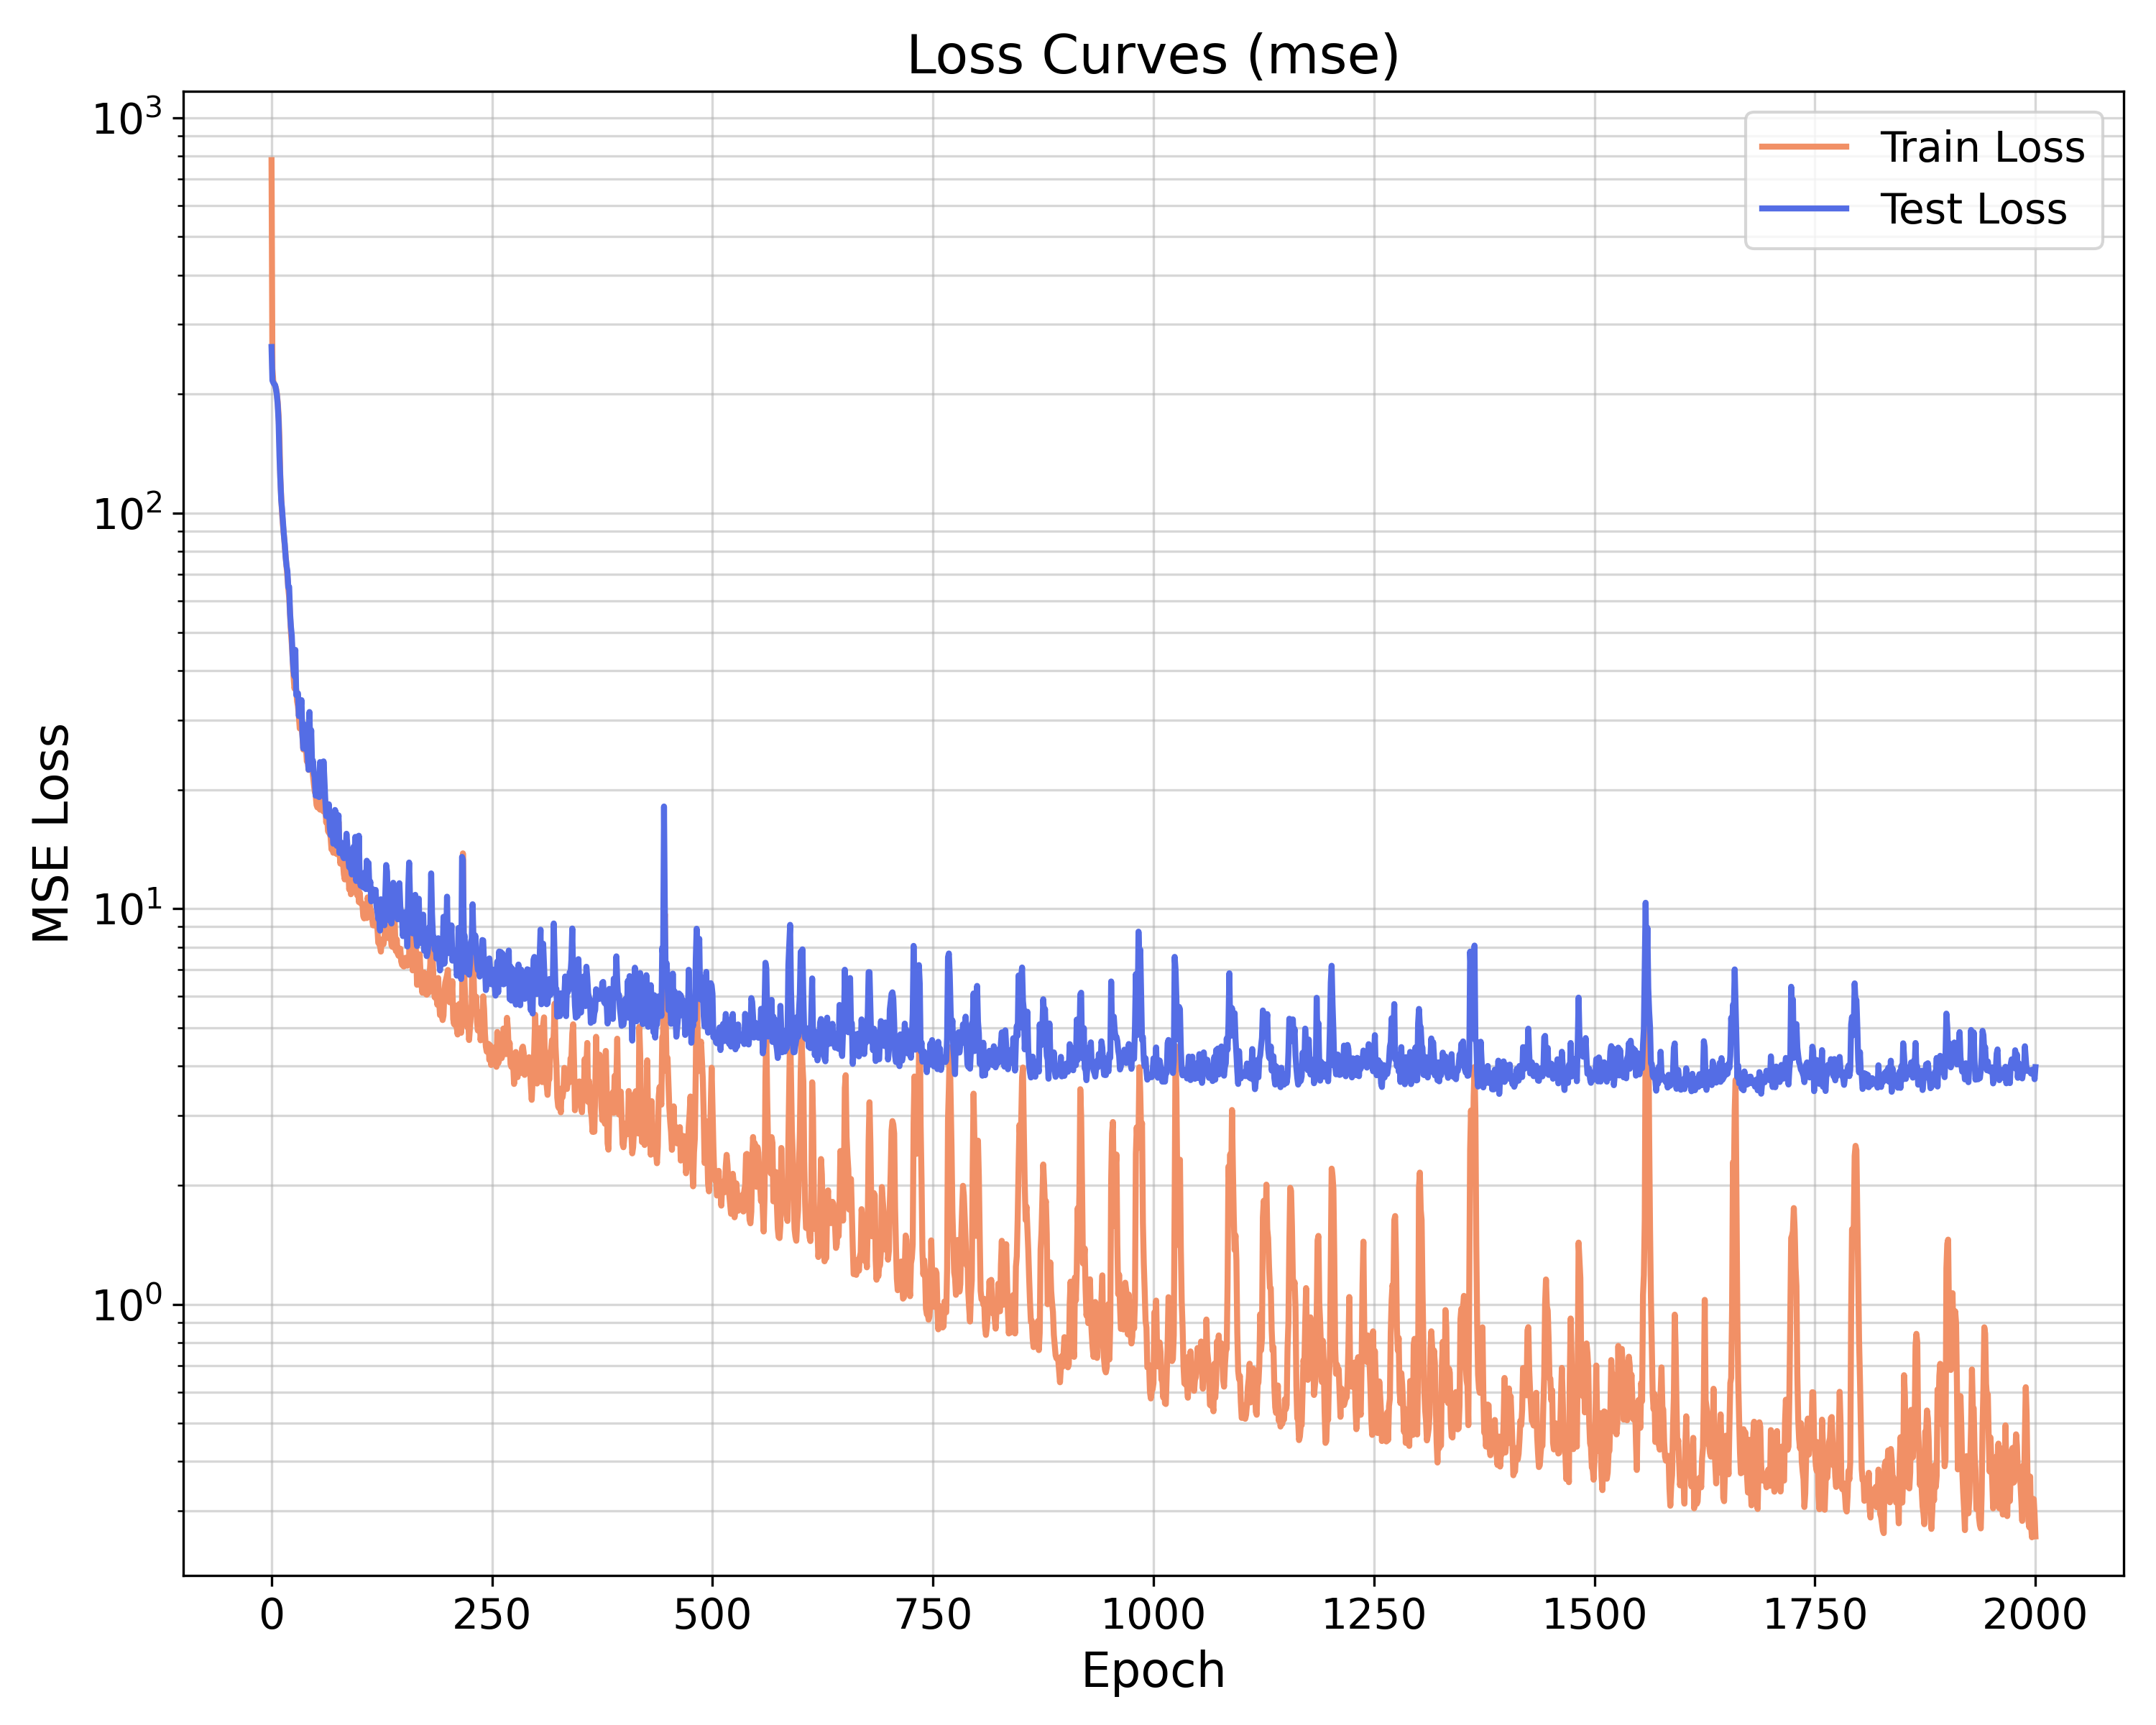
\includegraphics[width=\textwidth]{img/FH_model/BA_Network/FNO/loss_plot_fixed_S=42_N=300.png}
        \caption{$N=300$}
    \end{subfigure}
    \hfill
    \begin{subfigure}[b]{0.32\textwidth}
        \centering
        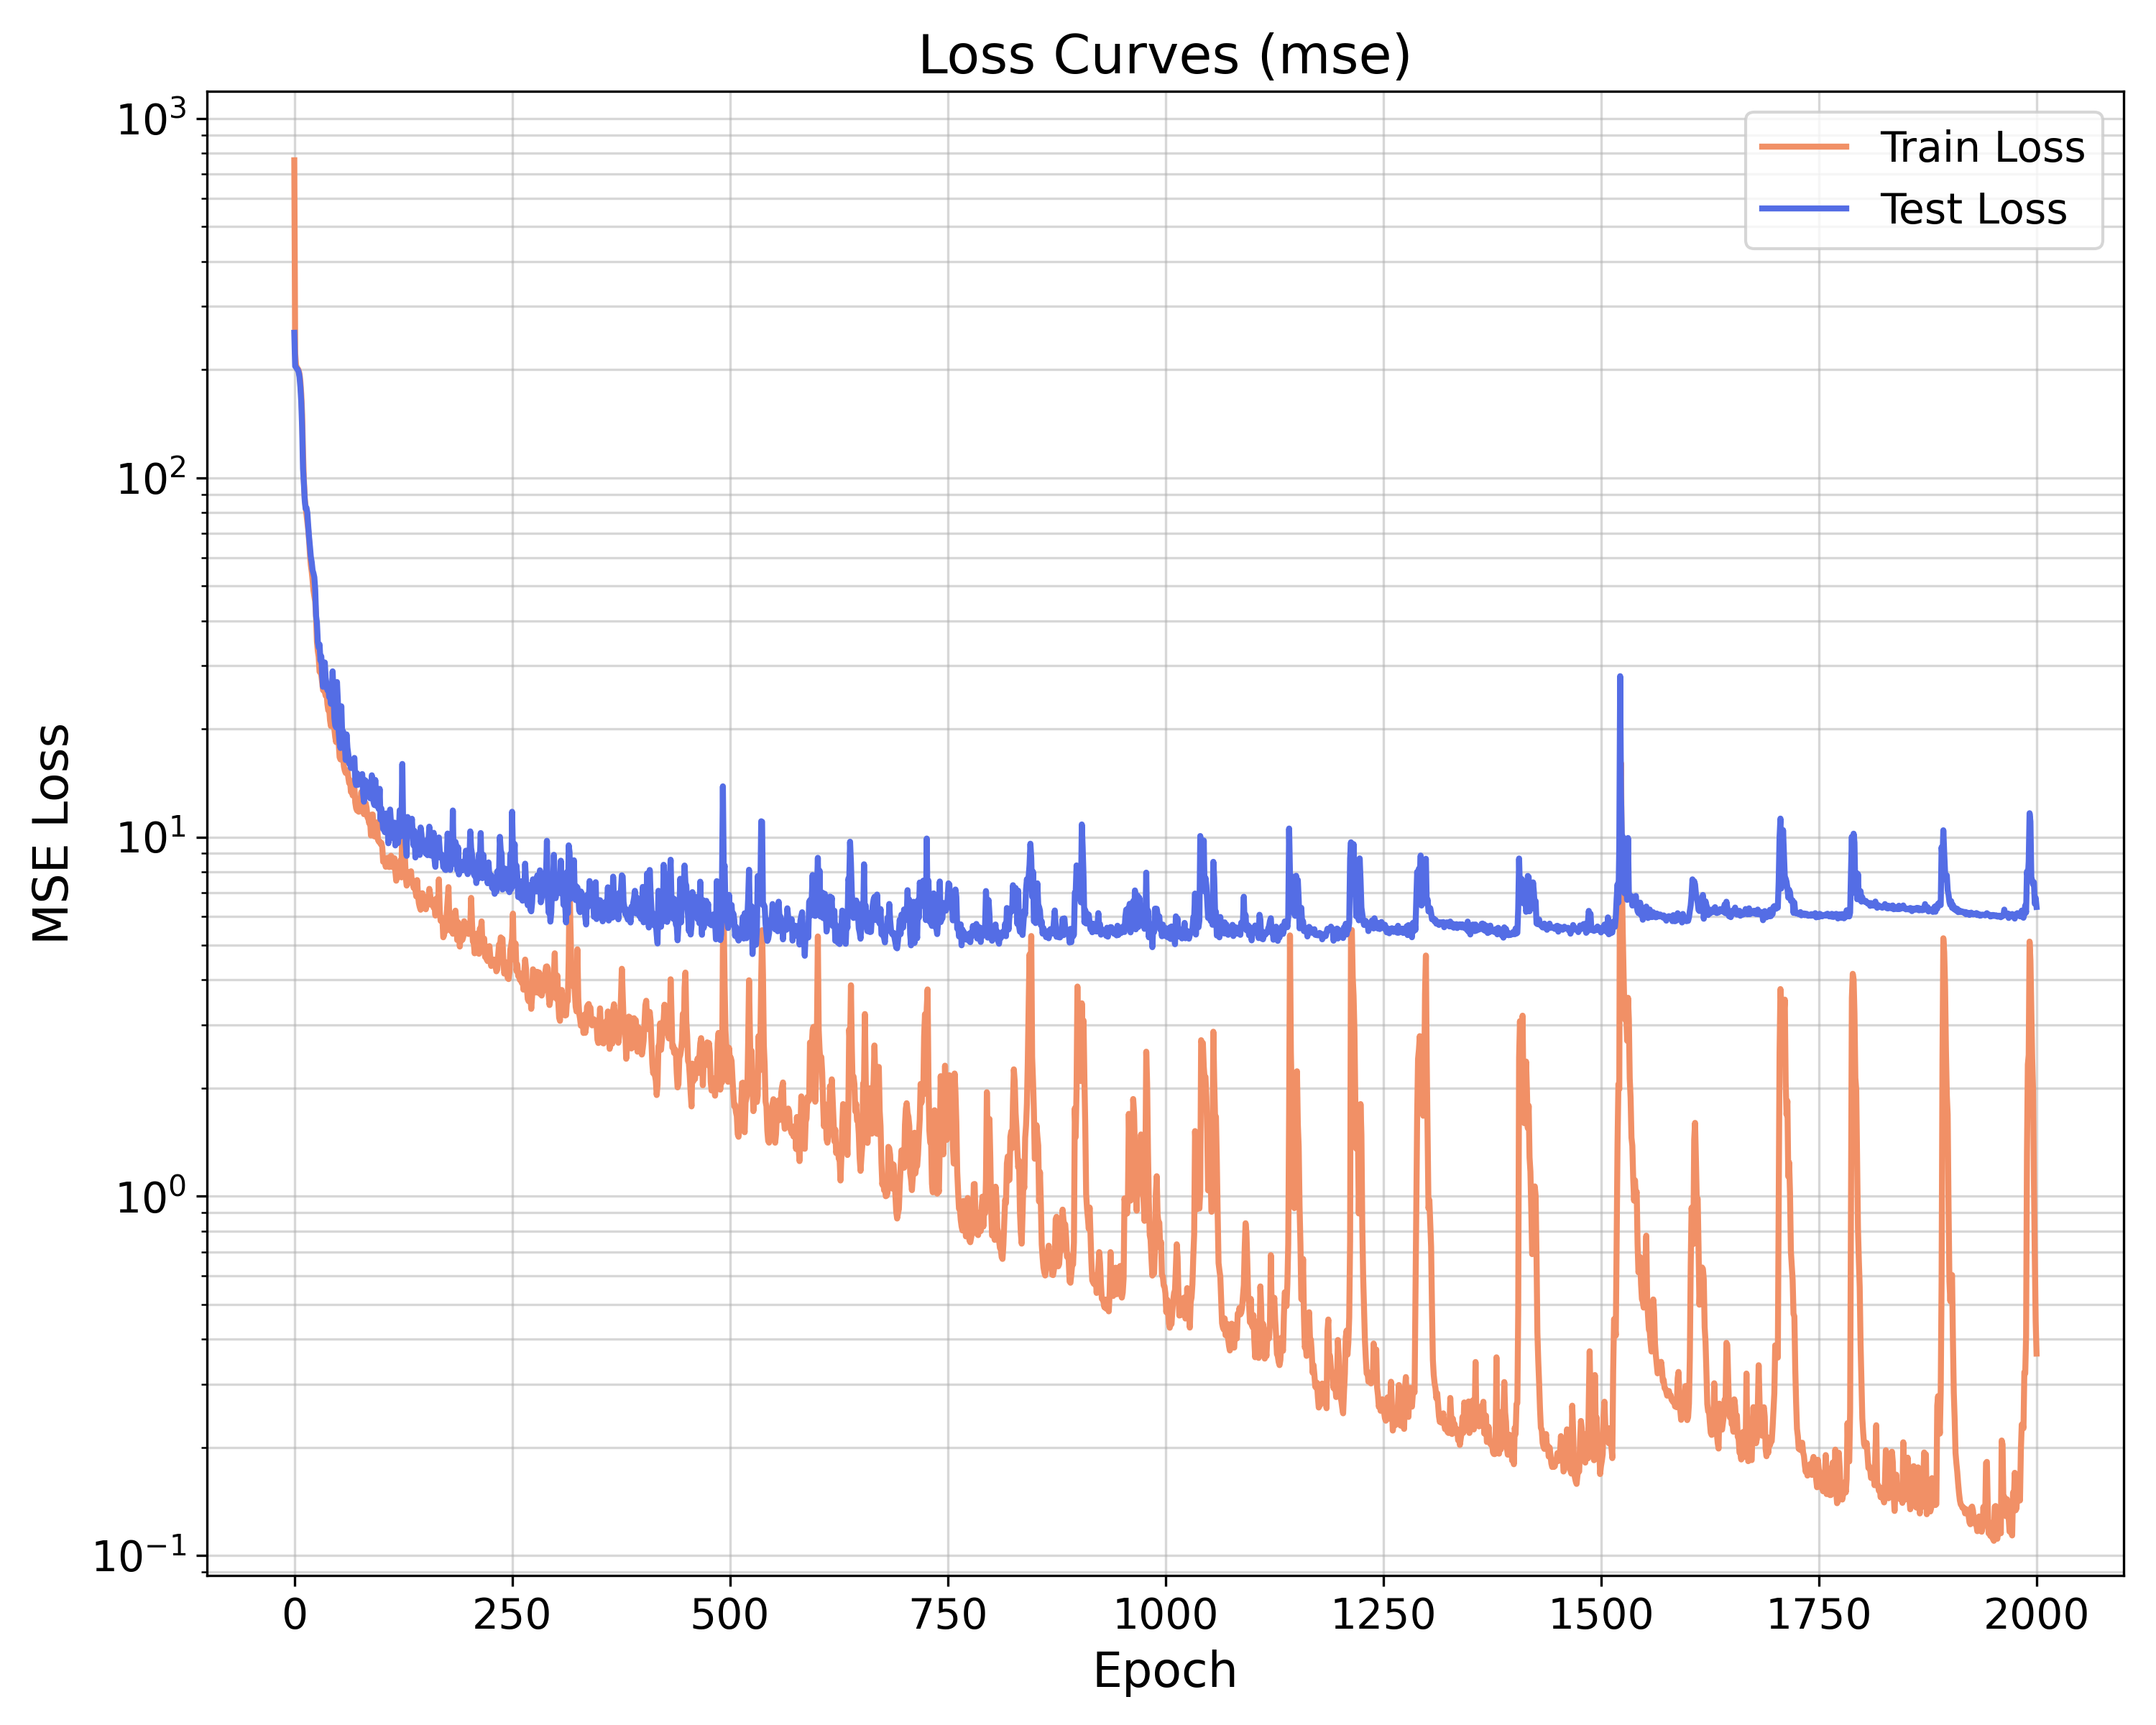
\includegraphics[width=\textwidth]{img/FH_model/BA_Network/FNO/loss_plot_fixed_S=42_N=400.png}
        \caption{$N=400$}
    \end{subfigure}
    \hfill
    \begin{subfigure}[b]{0.32\textwidth}
        \centering
        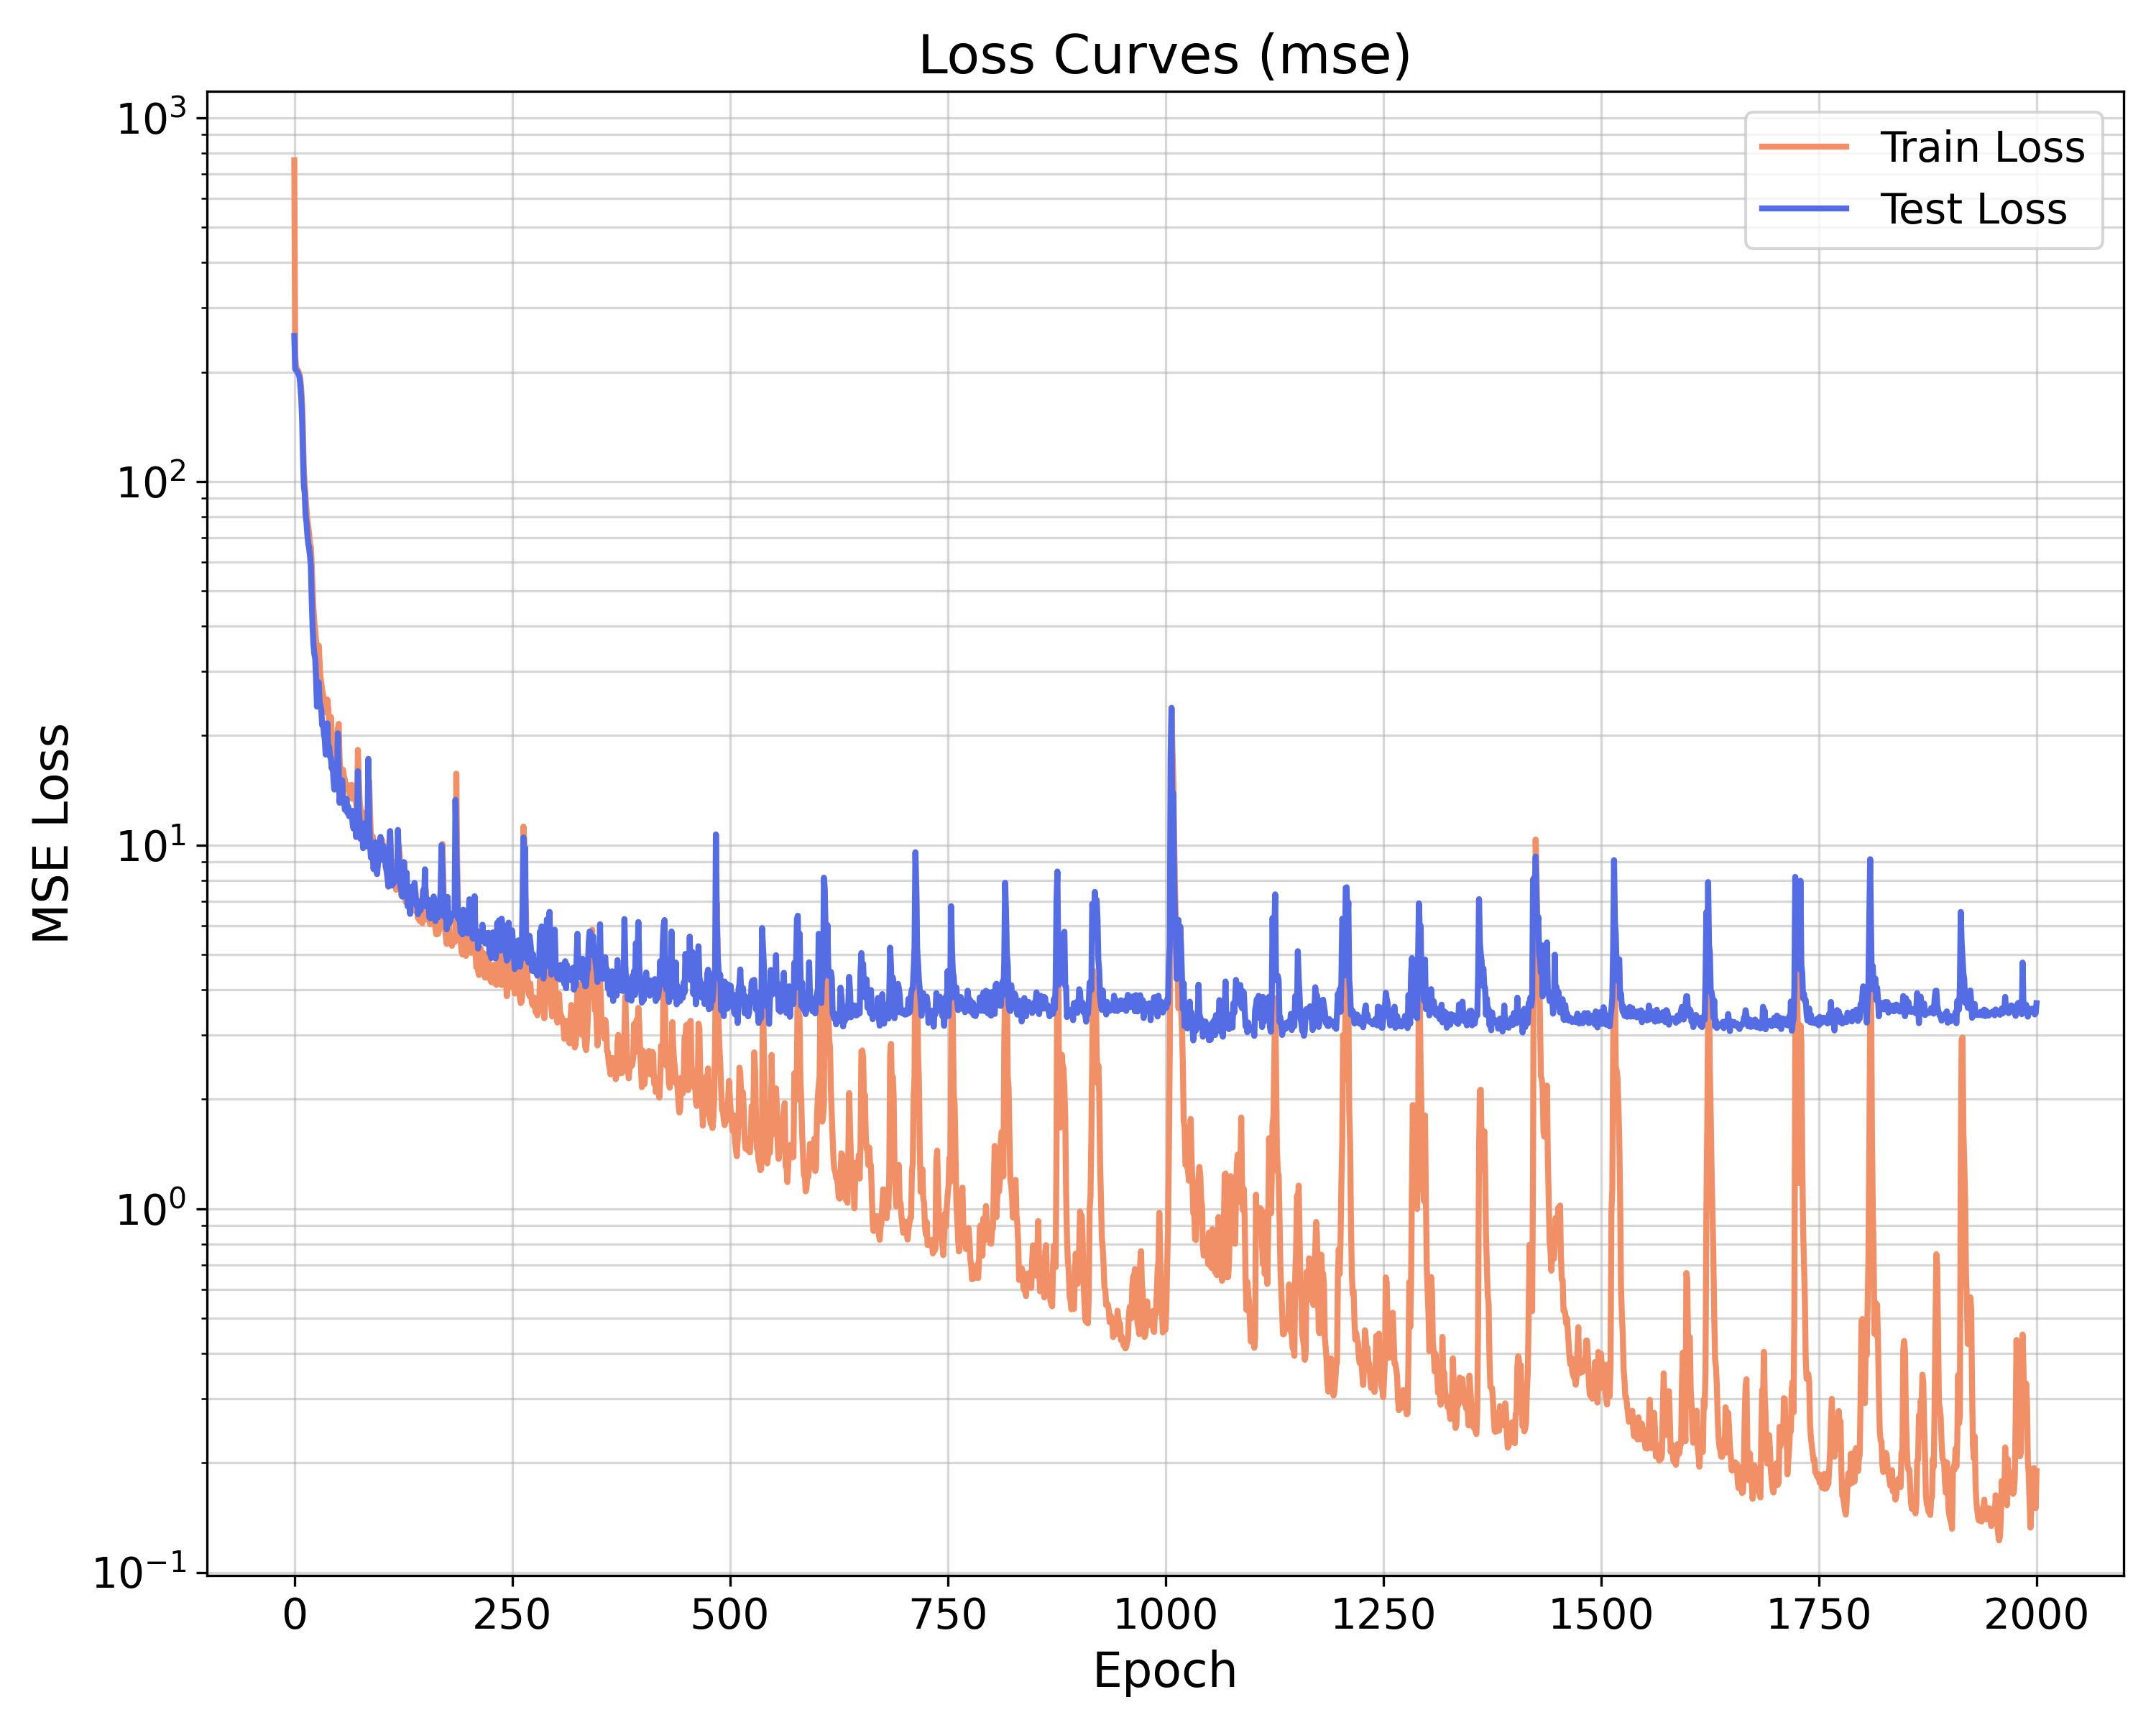
\includegraphics[width=\textwidth]{img/FH_model/BA_Network/FNO/loss_plot_fixed_S=42_N=500.png}
        \caption{$N=500$}
    \end{subfigure}
    
    \vspace{0.4cm}
    
    % --- Terza riga ---
    \begin{subfigure}[b]{0.32\textwidth}
        \centering
        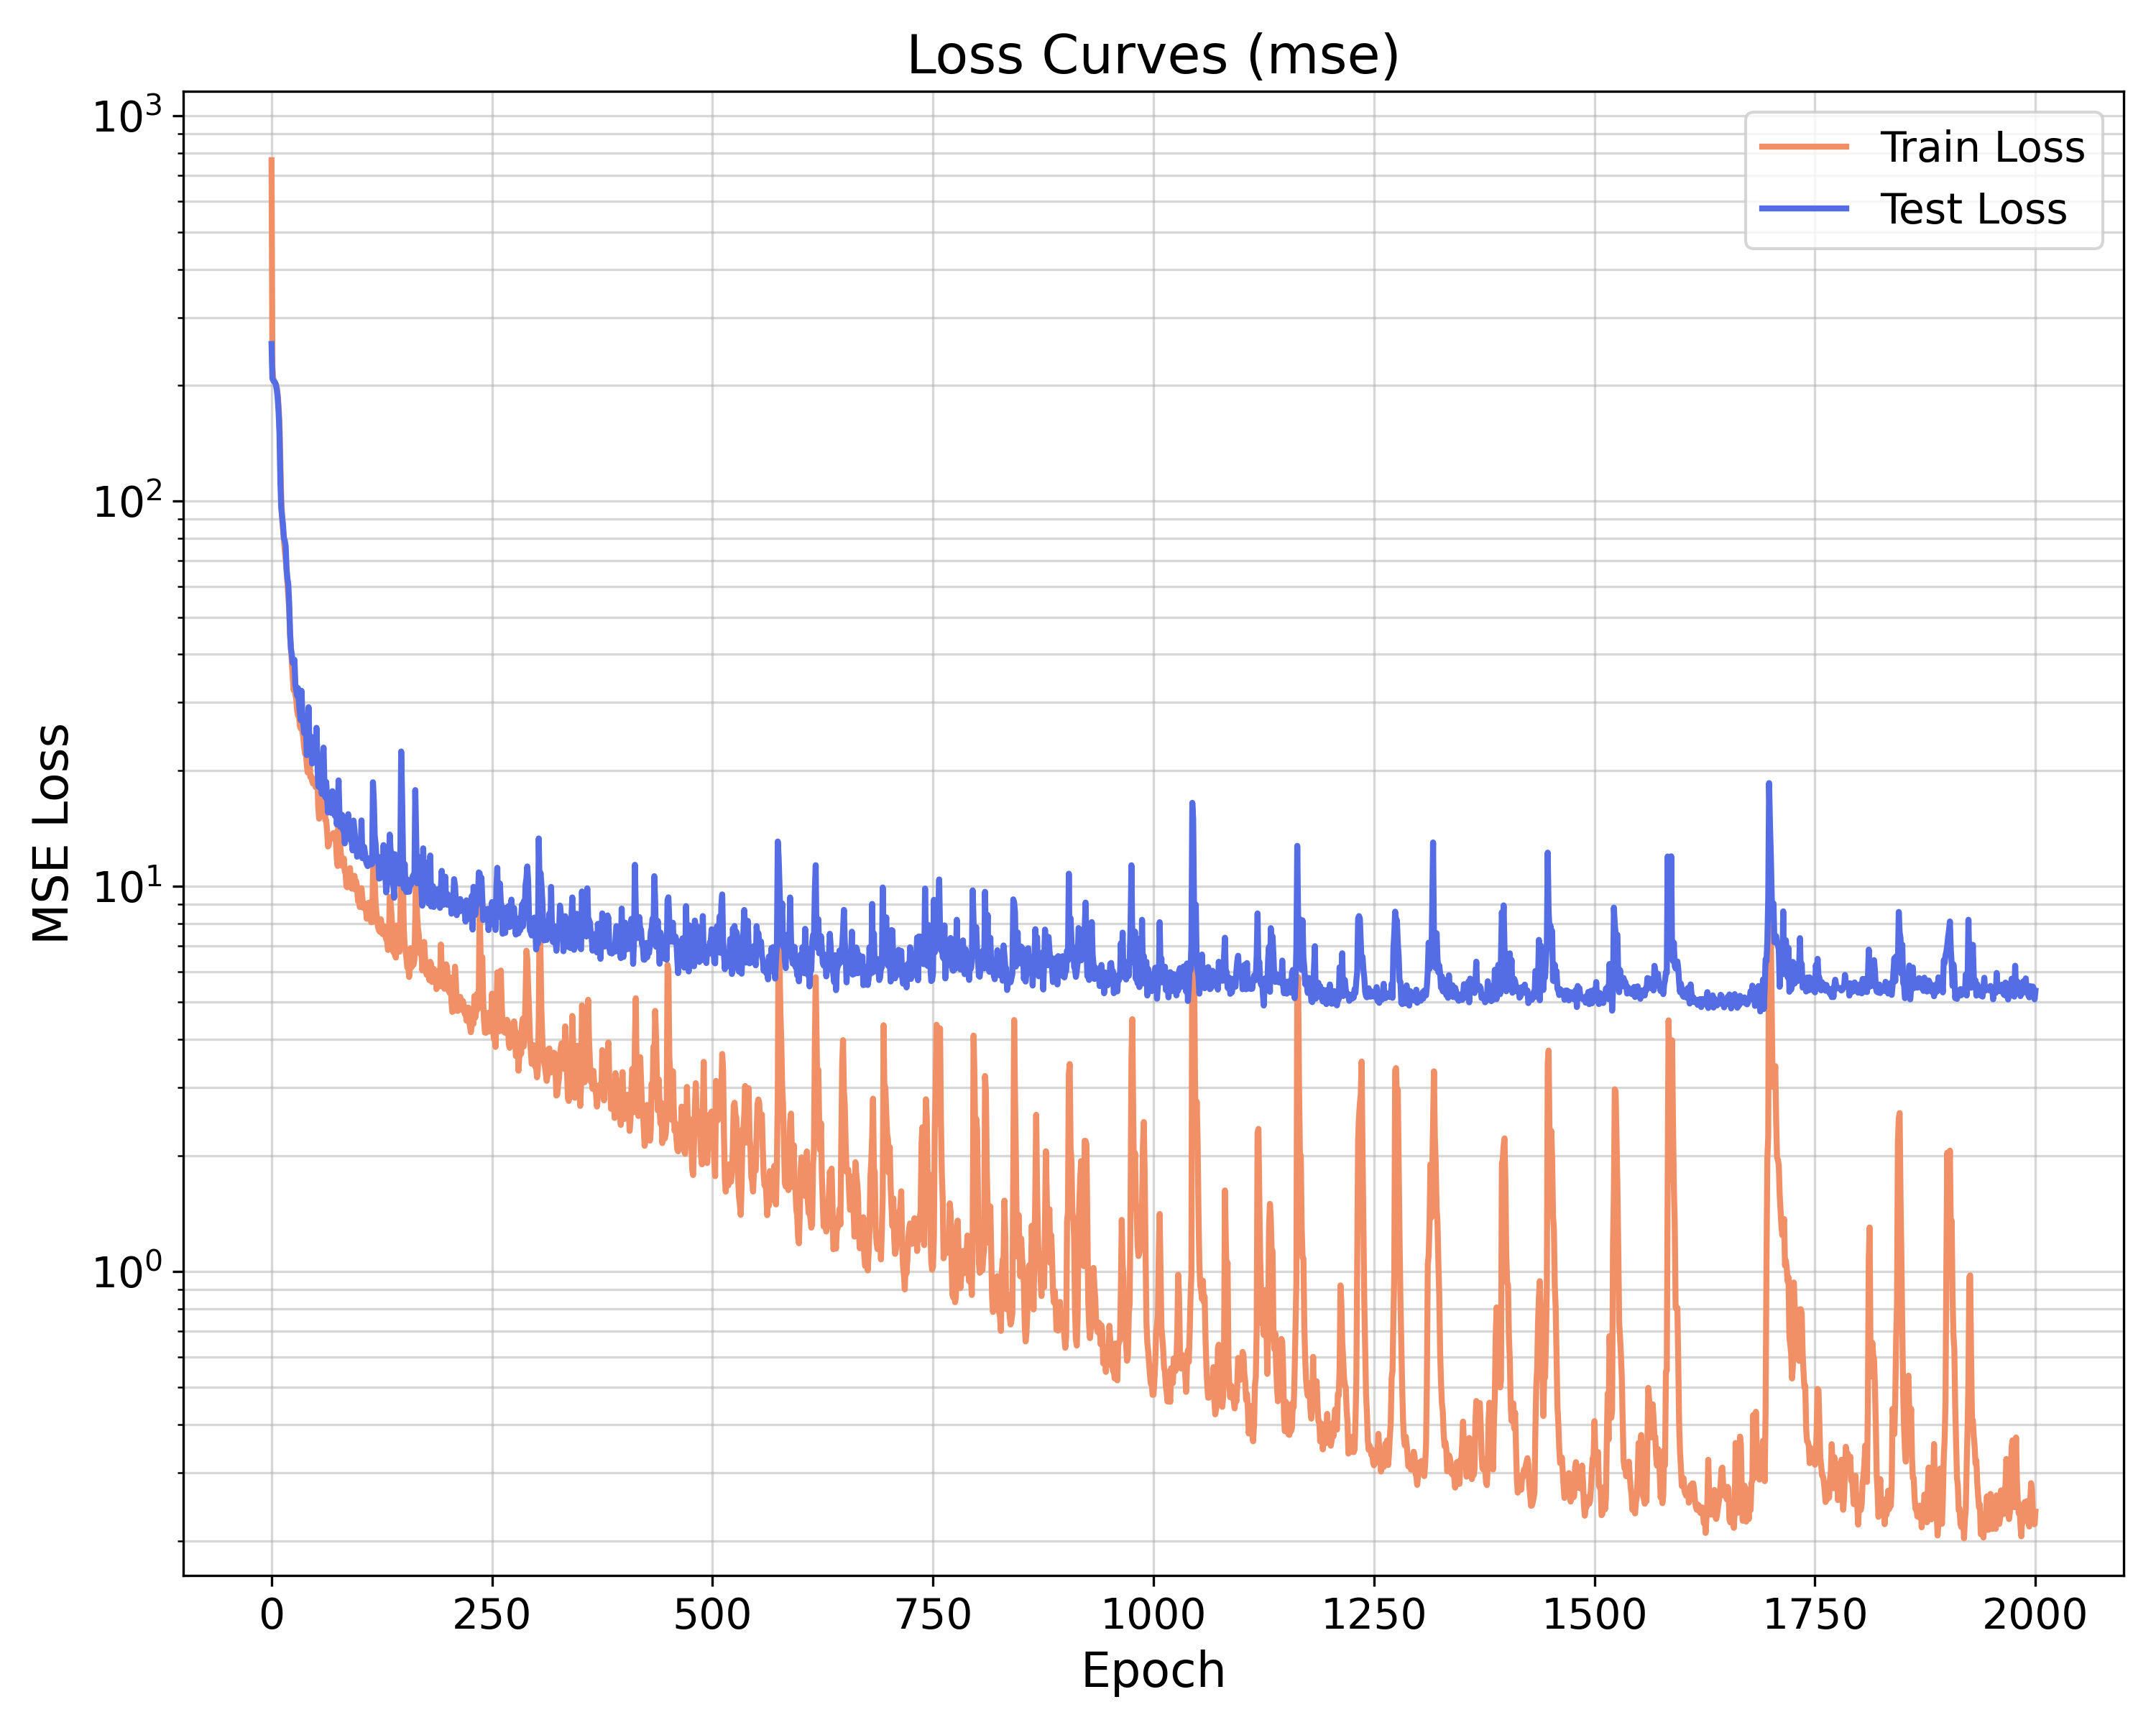
\includegraphics[width=\textwidth]{img/FH_model/BA_Network/FNO/loss_plot_fixed_S=42_N=600.png}
        \caption{$N=600$}
    \end{subfigure}
    \hfill
    \begin{subfigure}[b]{0.32\textwidth}
        \centering
        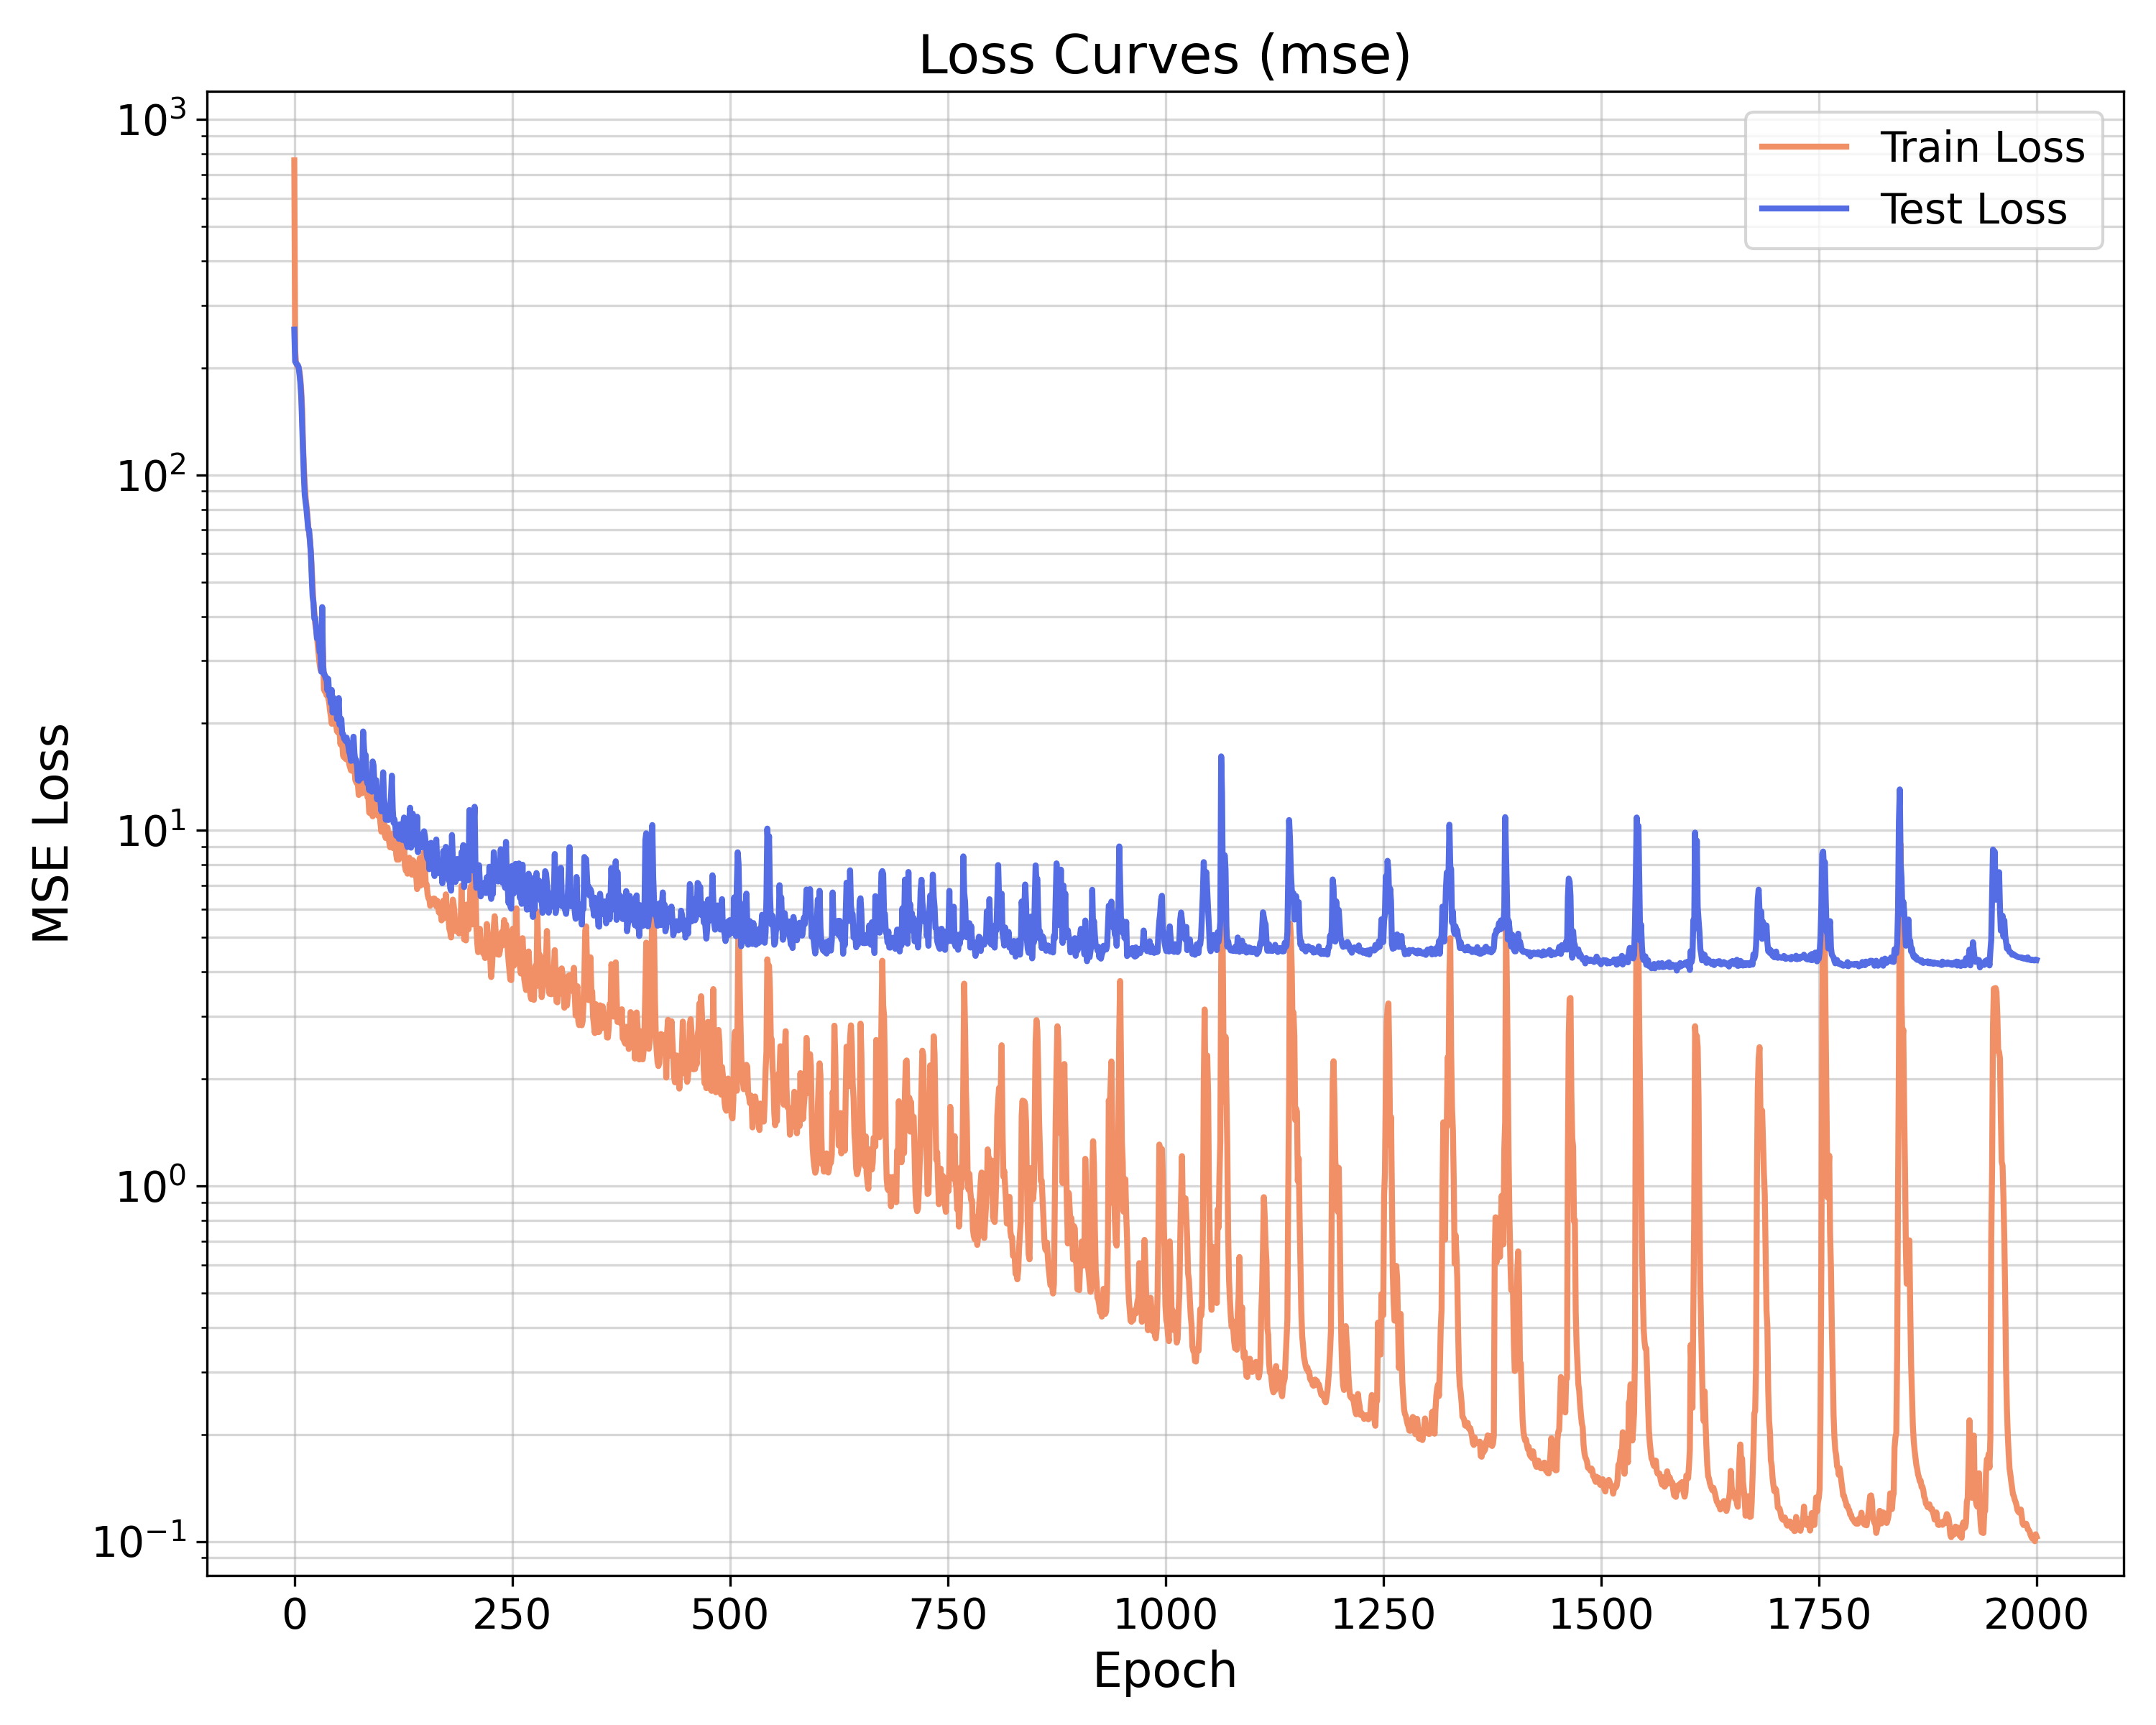
\includegraphics[width=\textwidth]{img/FH_model/BA_Network/FNO/loss_plot_fixed_S=42_N=700.png}
        \caption{$N=700$}
    \end{subfigure}
    \hfill
    \begin{subfigure}[b]{0.32\textwidth}
        \centering
        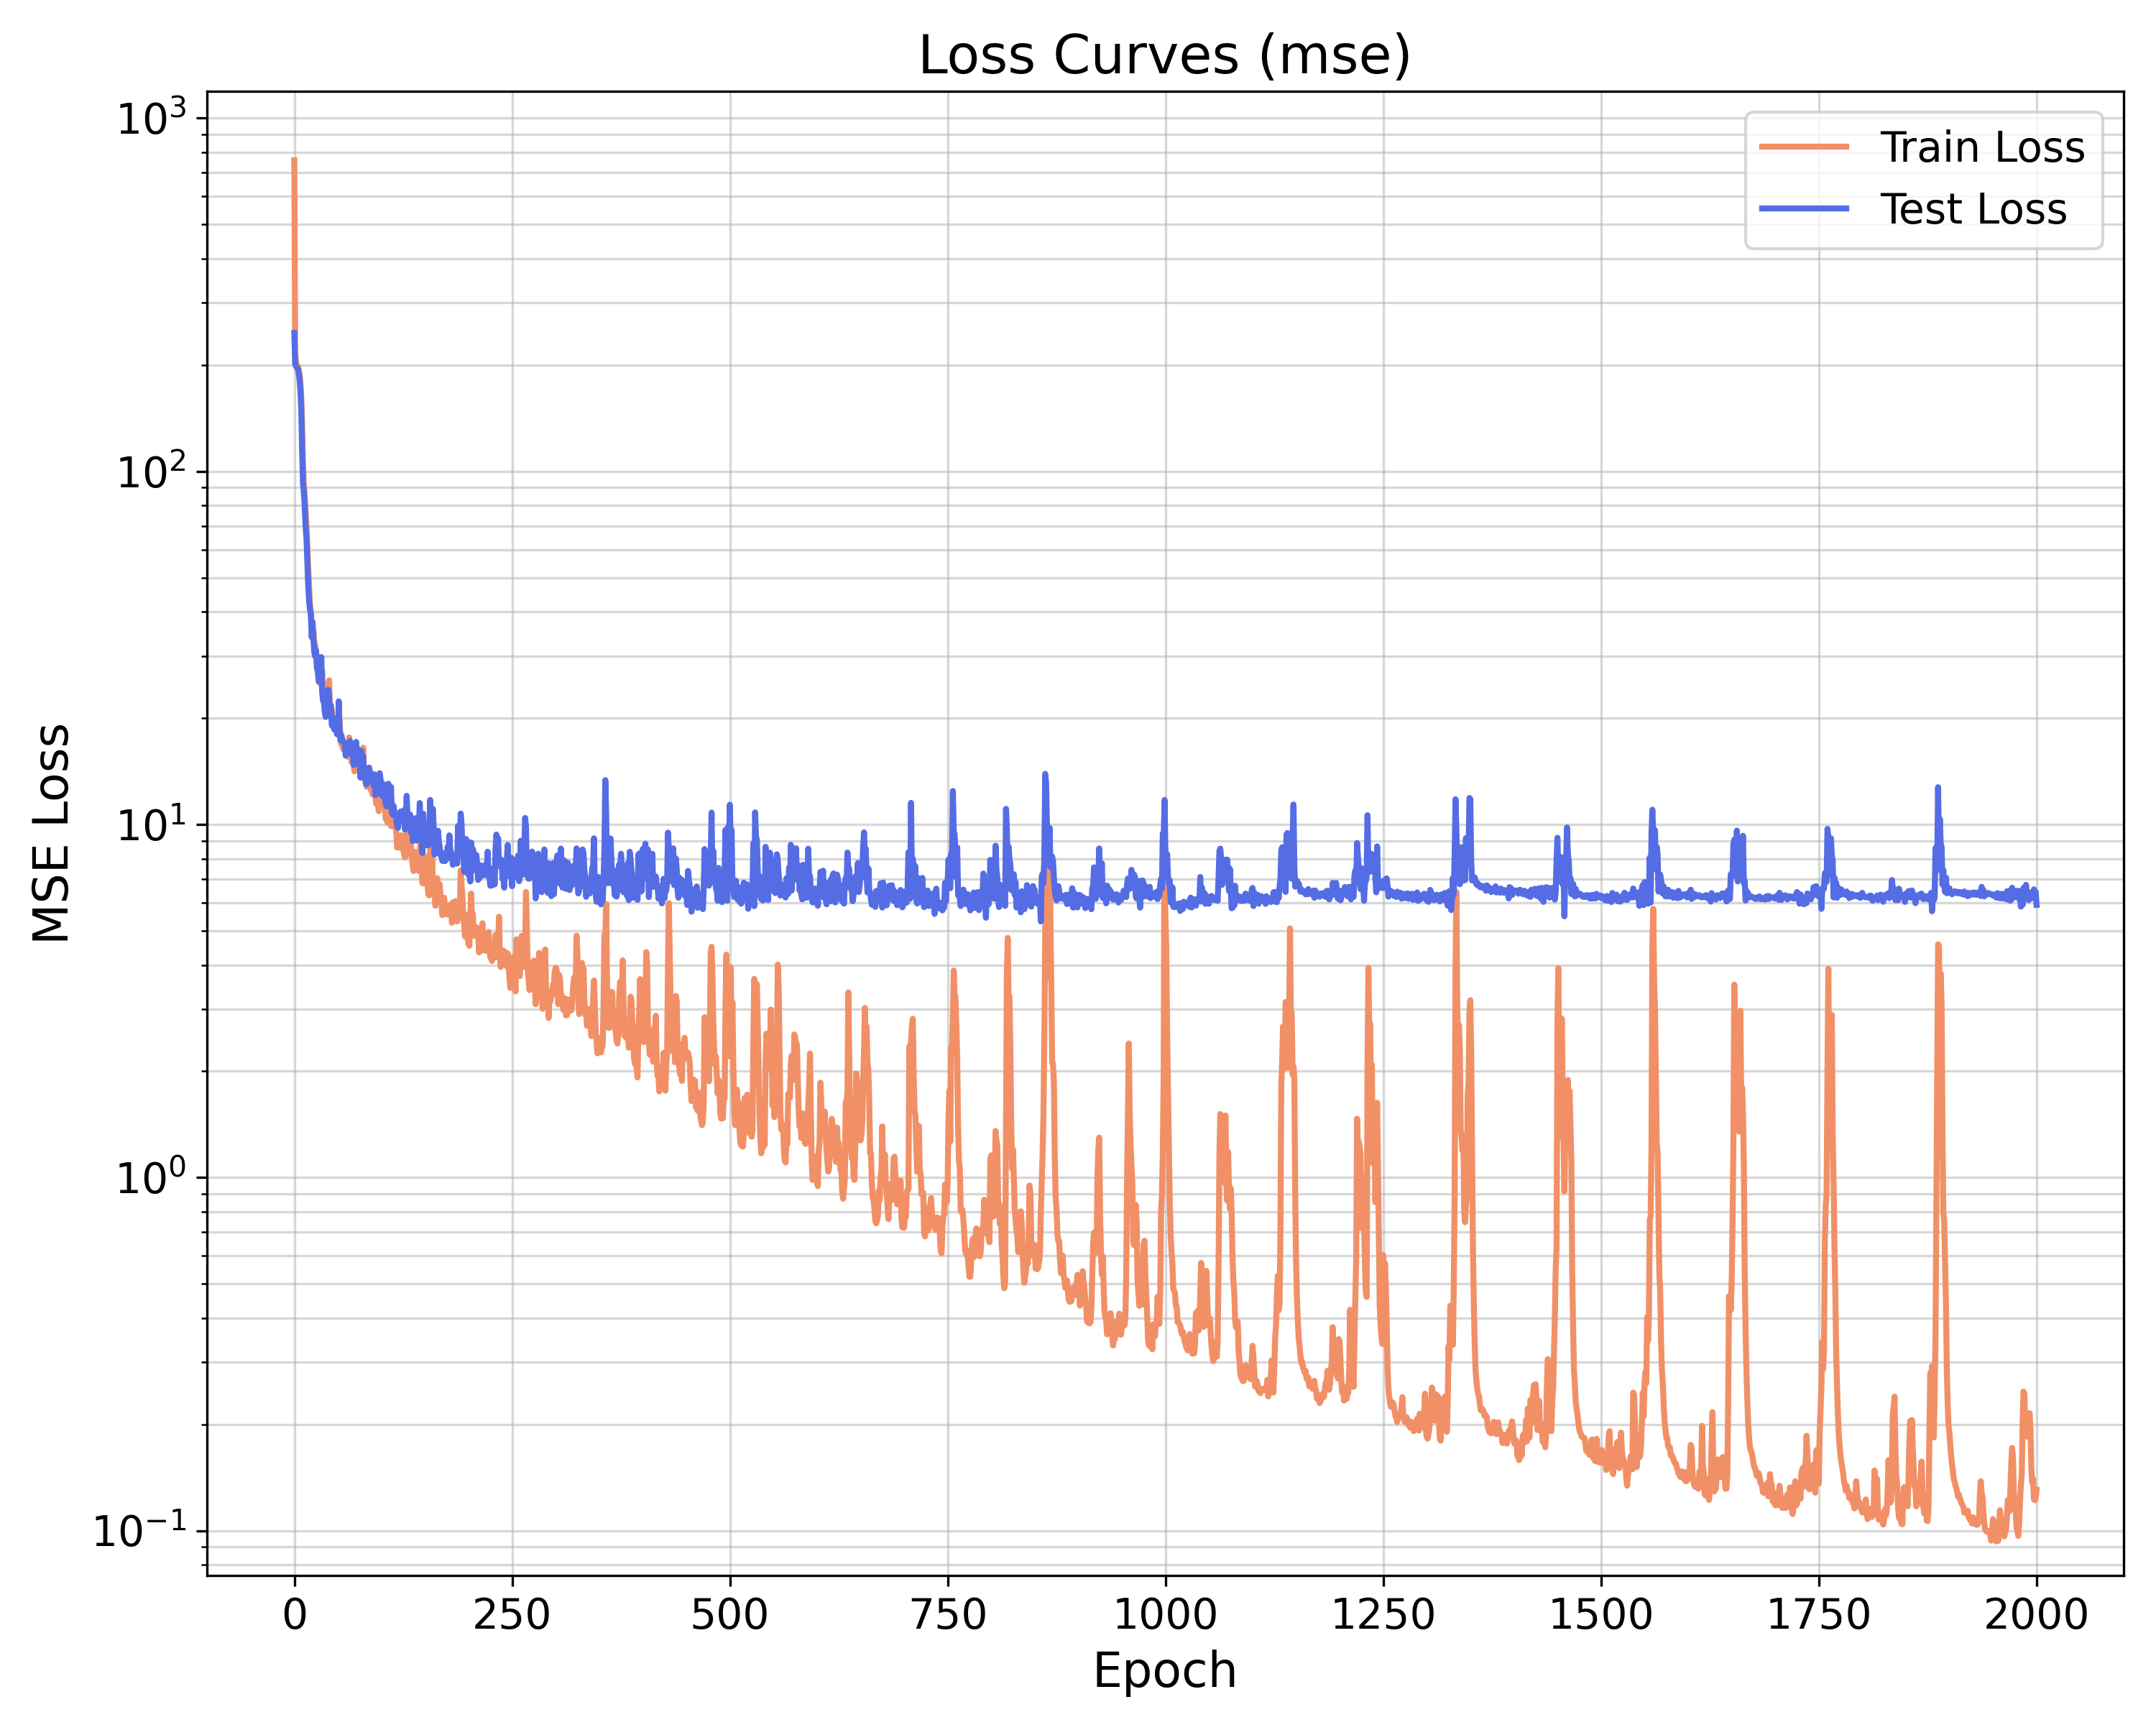
\includegraphics[width=\textwidth]{img/FH_model/BA_Network/FNO/loss_plot_fixed_S=42_N=800.png}
        \caption{$N=800$}
    \end{subfigure}
    
    \vspace{0.4cm}
    
    % --- Quarta riga ---
    \begin{subfigure}[b]{0.32\textwidth}
        \centering
        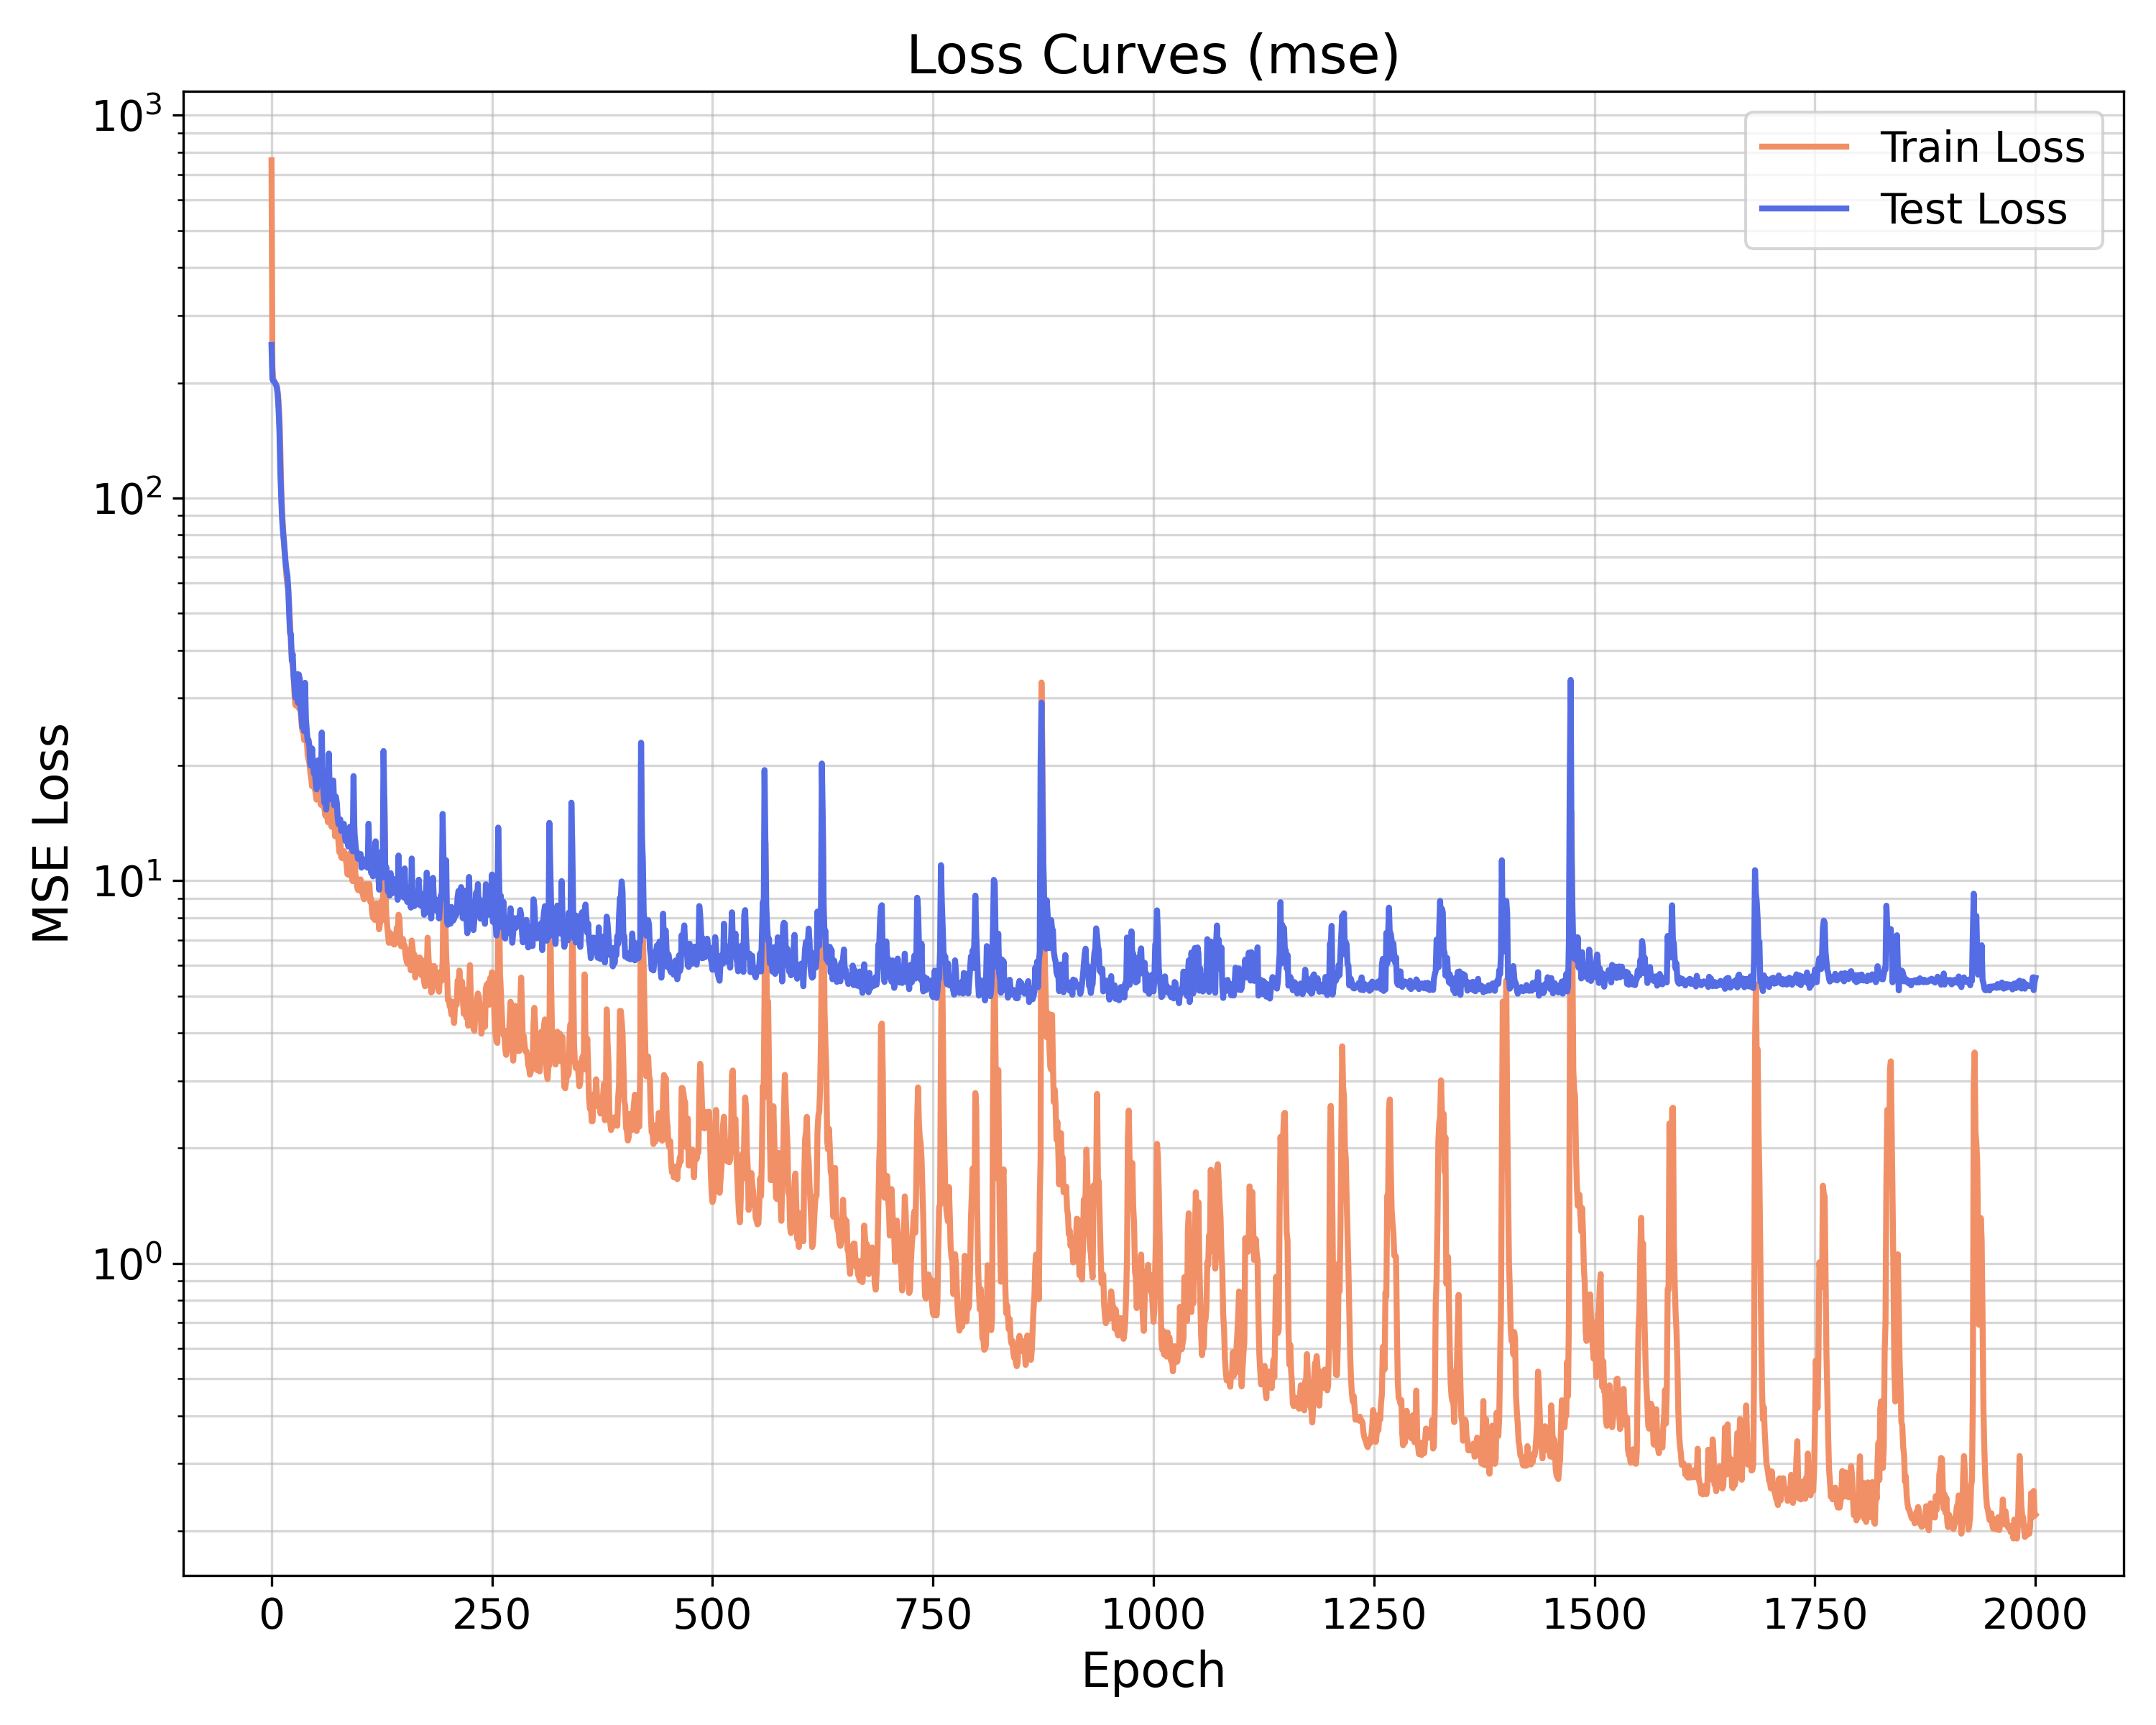
\includegraphics[width=\textwidth]{img/FH_model/BA_Network/FNO/loss_plot_fixed_S=42_N=900.png}
        \caption{$N=900$}
    \end{subfigure}
    \hfill
    \begin{subfigure}[b]{0.32\textwidth}
        \centering
        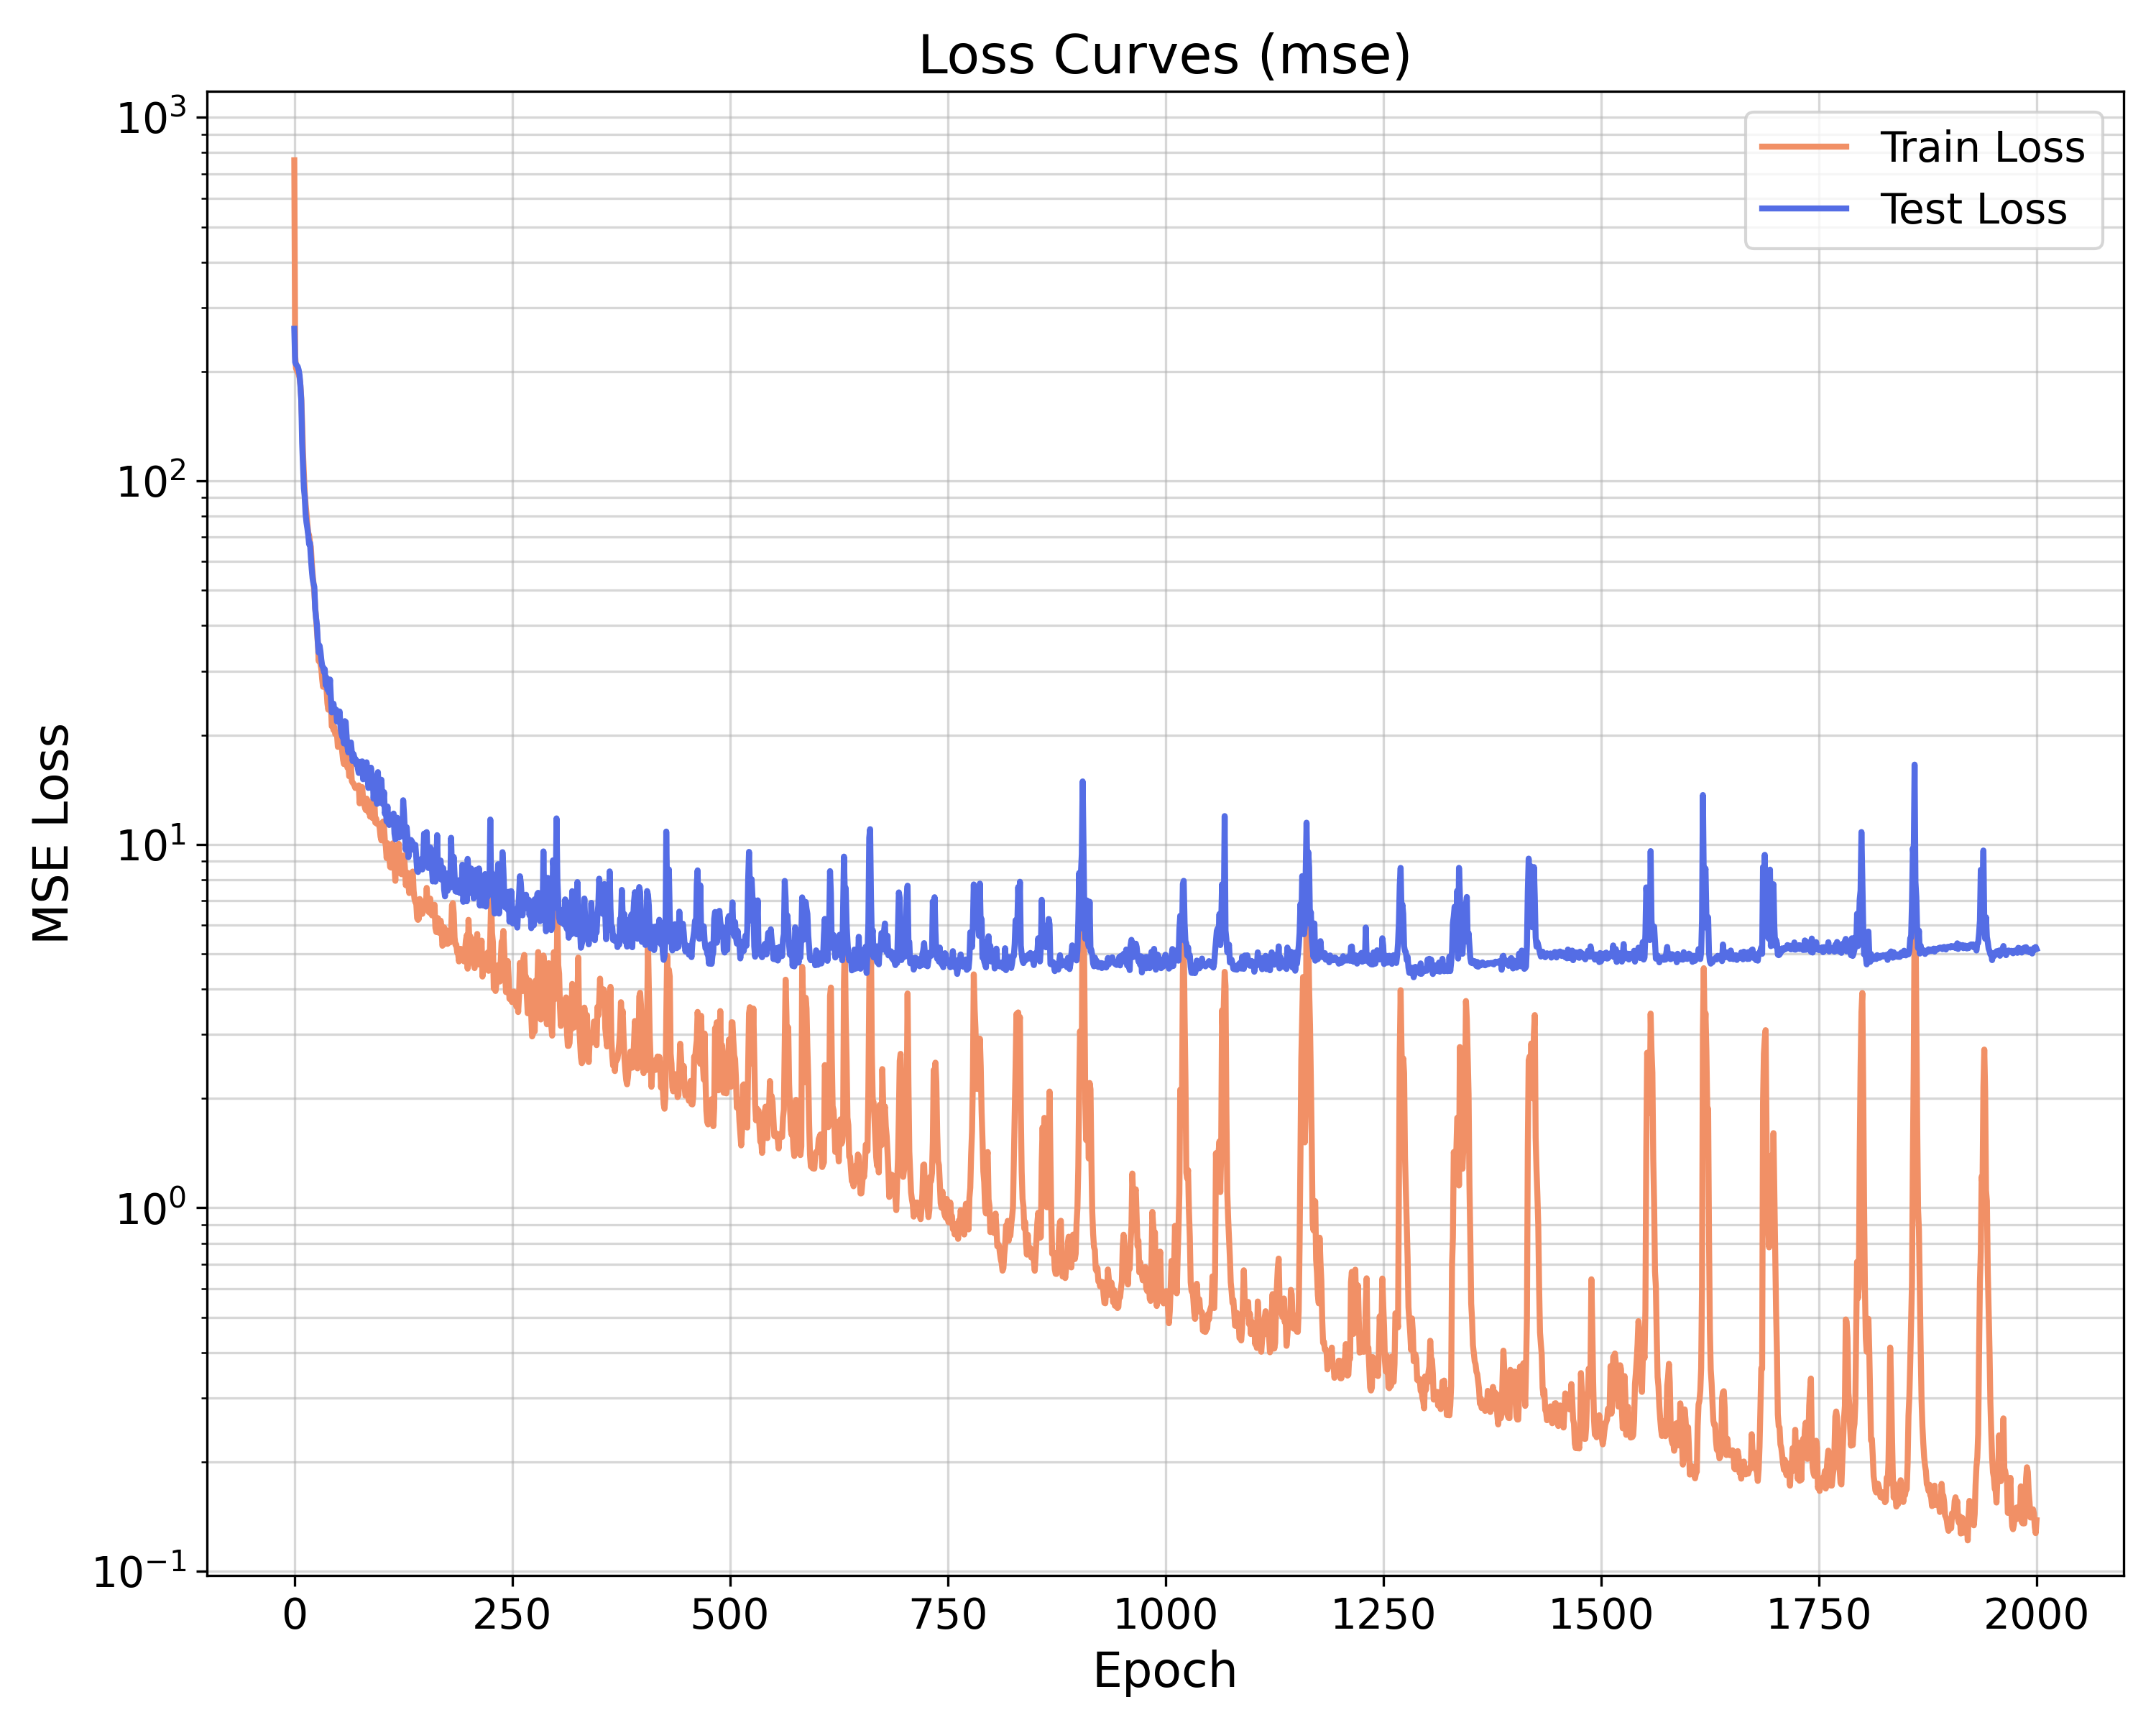
\includegraphics[width=\textwidth]{img/FH_model/BA_Network/FNO/loss_plot_fixed_S=42_N=1000.png}
        \caption{$N=1000$}
    \end{subfigure}
    \hfill
    \begin{subfigure}[b]{0.32\textwidth}
        \centering
        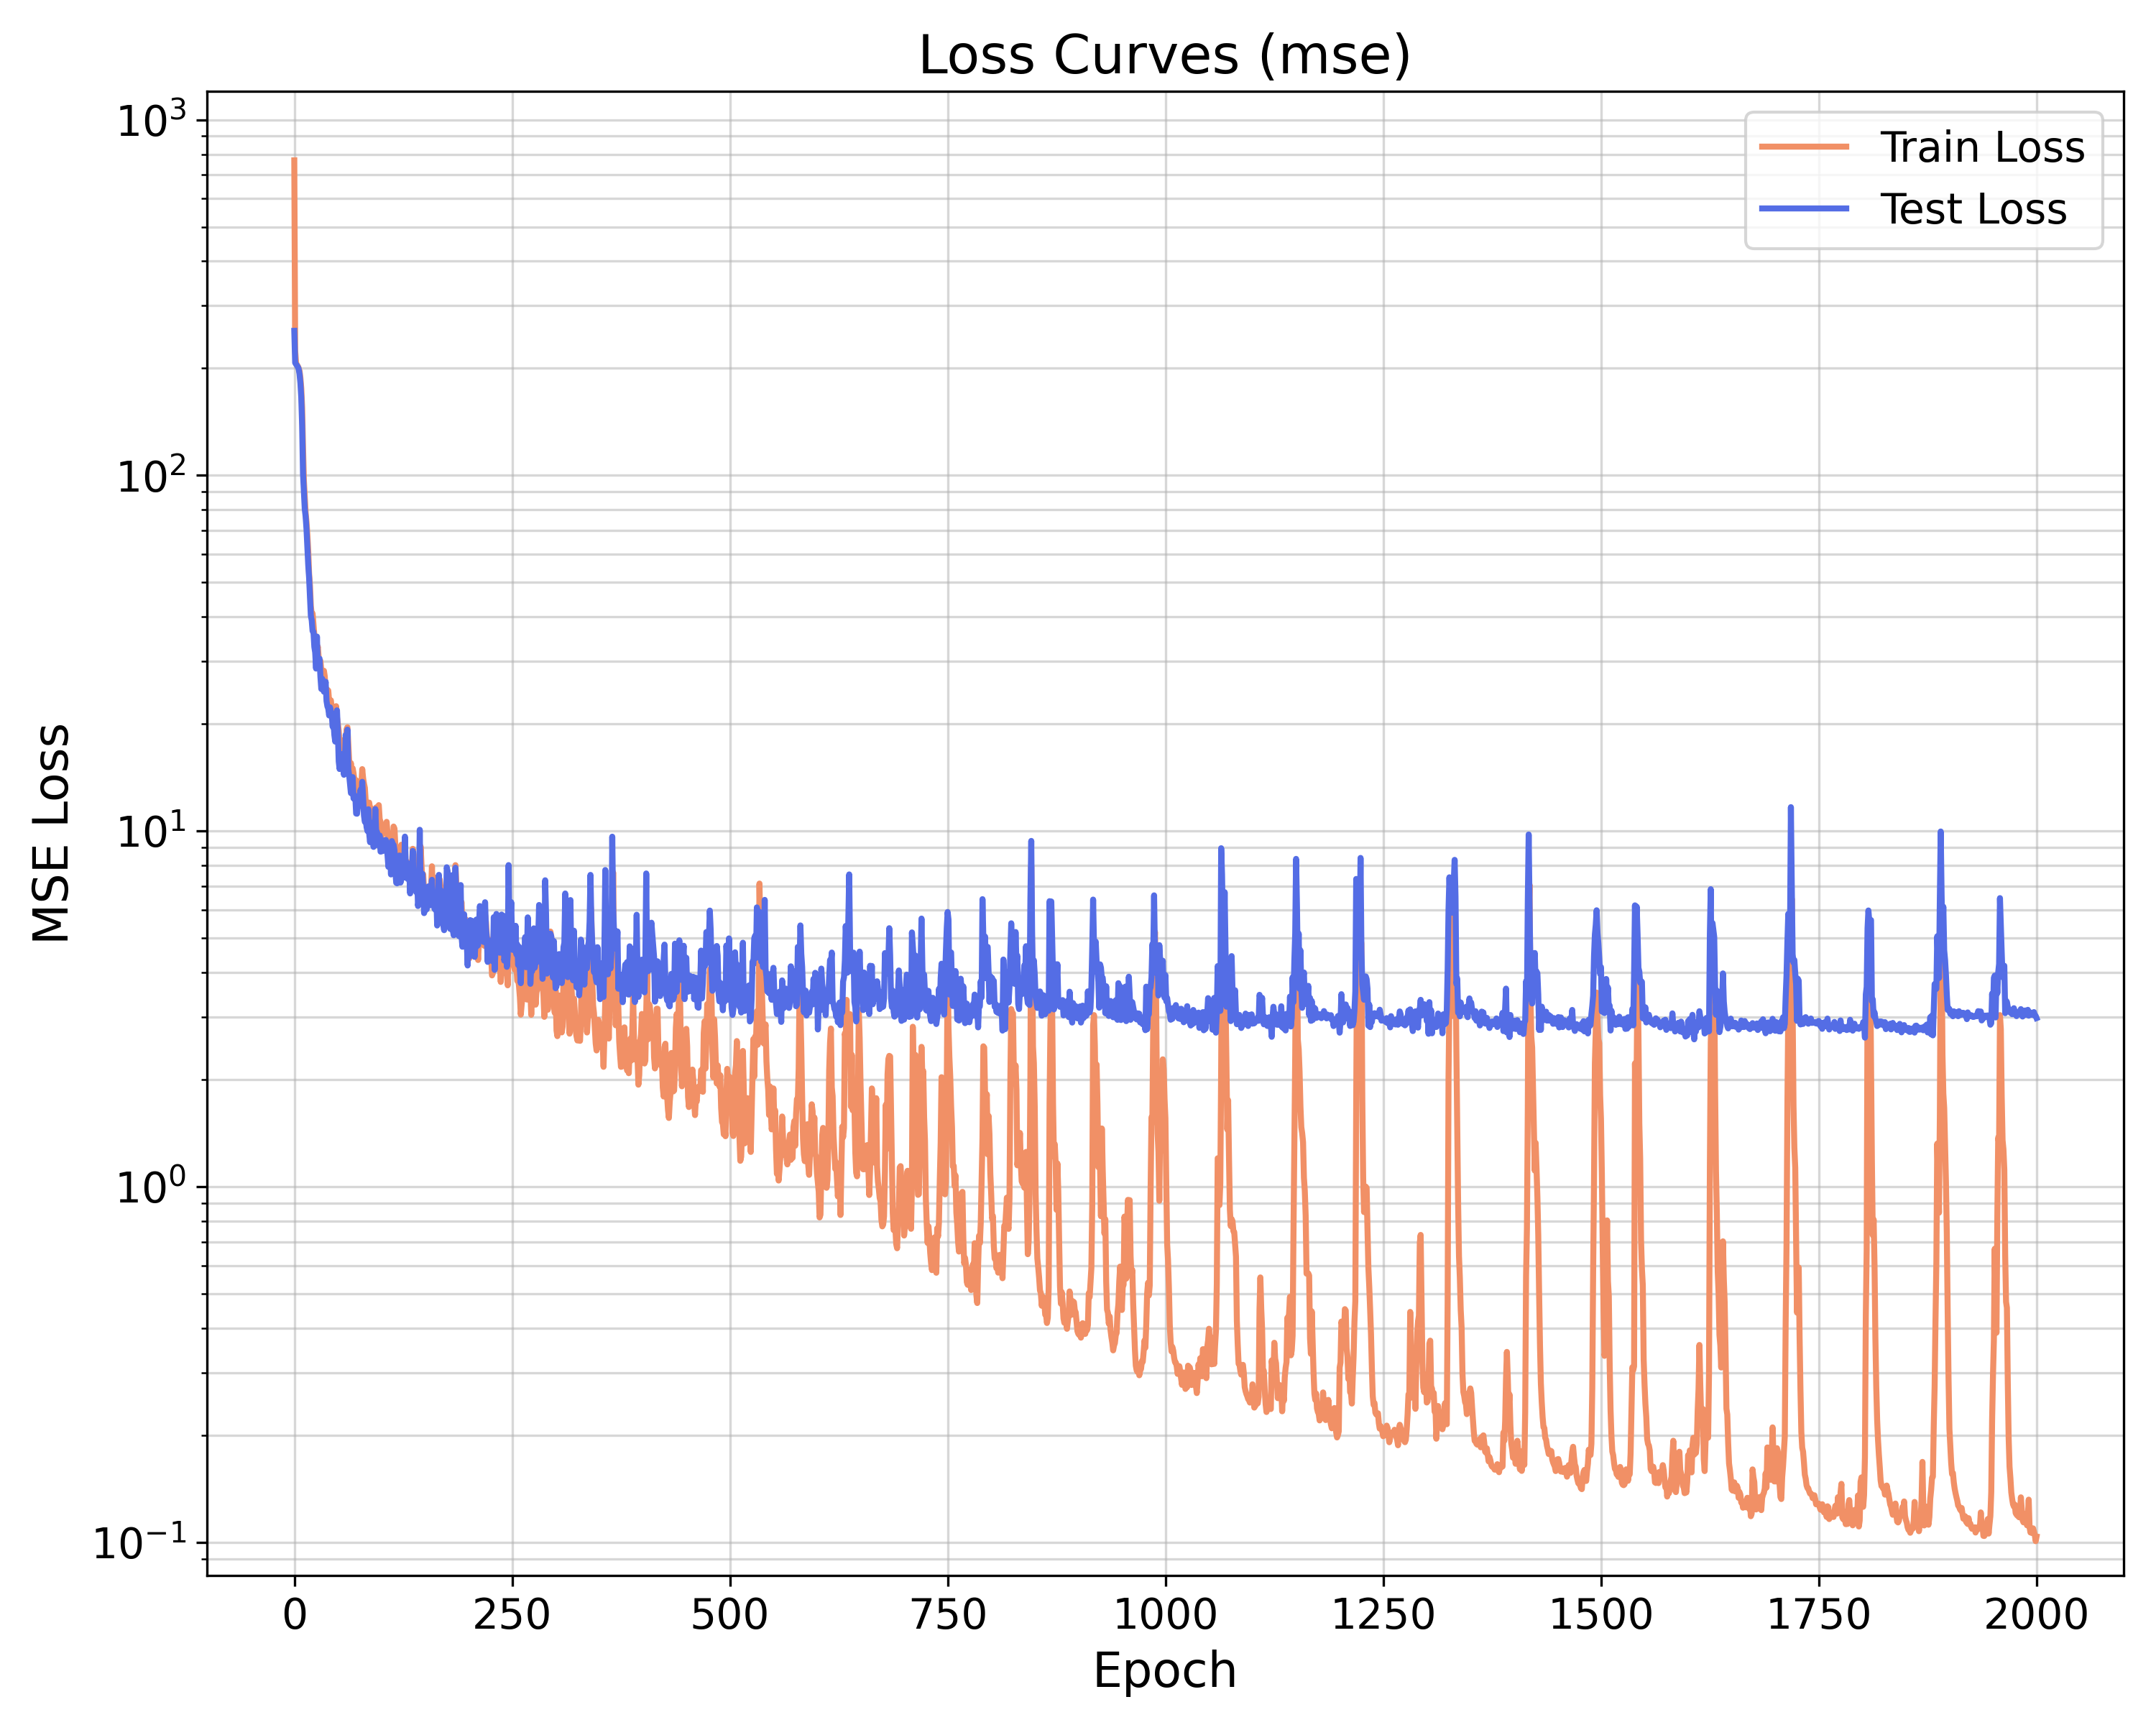
\includegraphics[width=\textwidth]{img/FH_model/BA_Network/FNO/loss_plot_fixed_S=42_N=2000.png}
        \caption{$N=2000$}
    \end{subfigure}
    
    \caption{Training and test loss convergence for different Barab\'asi-Albert network sizes ($N$).}
    \label{fig:ba_loss_grid}
\end{figure}


%% Il caso N=100 mi sembra un po' diverso dagli altri. Devo commentarlo? Forse c'è un path più breve tra input ed output.

\subsubsection{Performance across different sizes of the hidden network: Conclusion}

As we could see in the previous graphs, and in the summary Figure \ref{fig:fno_scaling_error} below, we can deduce that (at least for the sizes considered) the FNO generalizes well the deterministic dynamics. This remarkable scalability may also be due to the discretization-invariant nature of this architecture.
% In fact we performed some test where we trained on a dataset with hidden network size $N_1$ and tested on another $N_2$ and we still got good results.
A future extension could be to investigate if this good behavior persists even if noise is introduced into the system.

\begin{figure}[htbp]
    \centering
    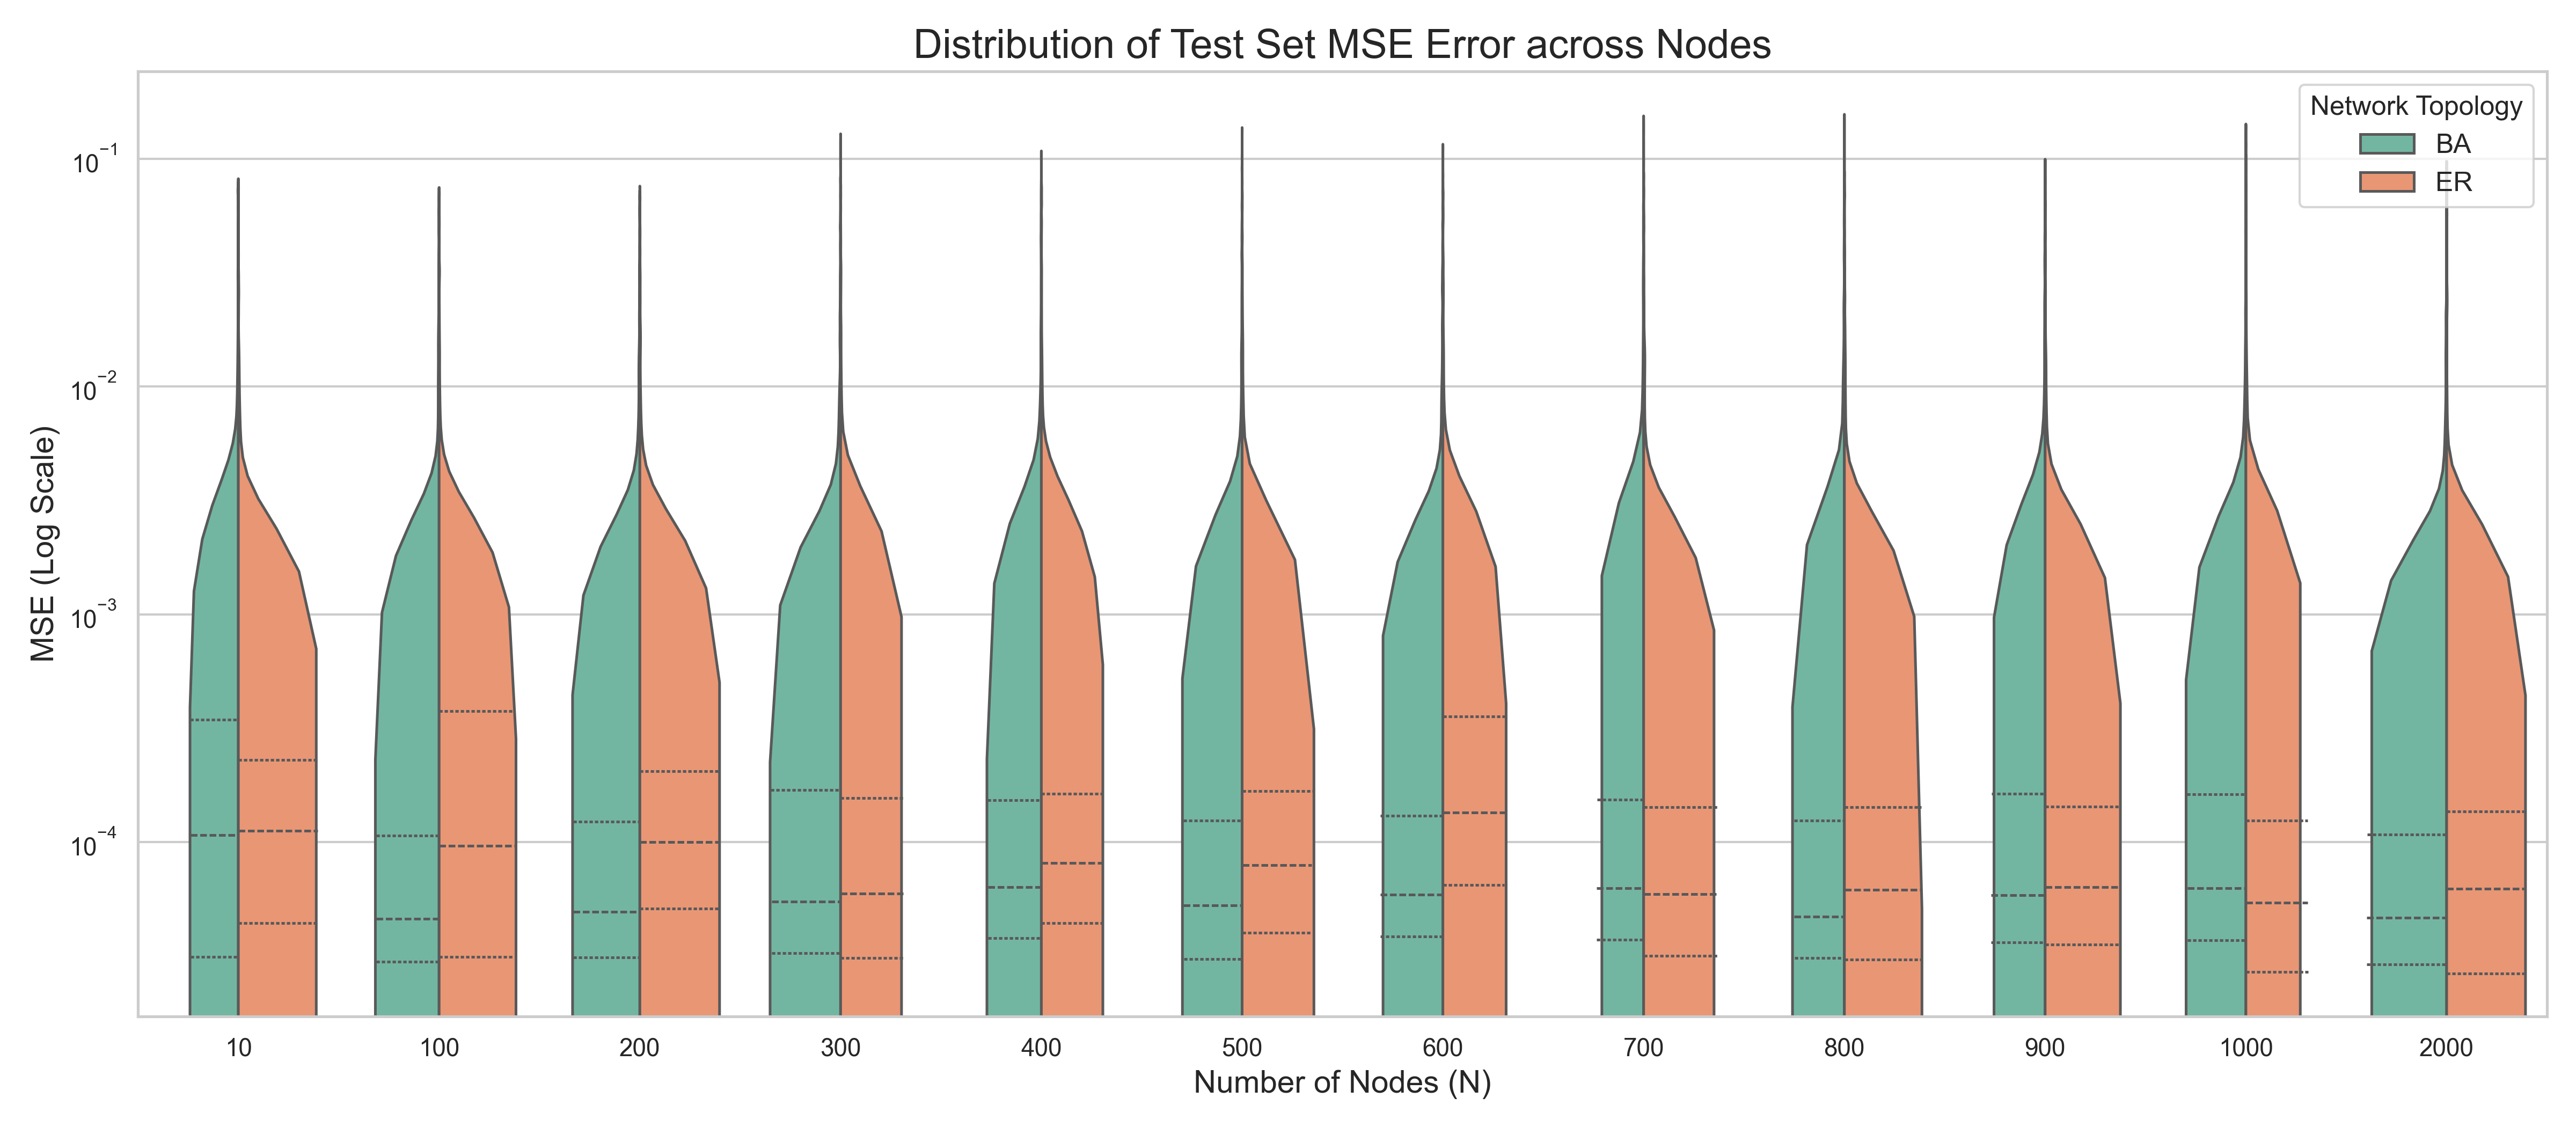
\includegraphics[width=0.8\textwidth]{img/FH_model/error_FNO_scalingN.png}
    \caption{Summary of the FNO performance across different network sizes ($N$). The plot compares the mean error scaling for both Erd\H{o}s-R\'enyi (ER) and Barab\'asi-Albert (BA) topologies, demonstrating the robustness and scalability of the architecture.}
    \label{fig:fno_scaling_error}
\end{figure}

%Test statistico?

%Collegamento con il teorema di Takens?

\subsection{C. Elegans connectonome}

\section{Dependence on the diffusion coefficient $\sigma$}

During the experiments presented in the previous sections, it became essential to understand how to appropriately tune the diffusion coefficient $\sigma$ as a function of the hidden network size $N$. In fact, if we maintain $\sigma$ fixed while $N$ increases, the transmitted energy dissipates and the output signal progressively attenuates until it completely dies out (a phenomenon akin to dynamical quenching). An initial numerical investigation suggested that the correct scaling to preserve the macroscopic dynamical regime is $\sigma = \mathcal{O}(N)$.

% Anche qui mi sa che dovrei rigenerare il grafico con le label in inglese
\begin{figure}[htbp]
    \centering
    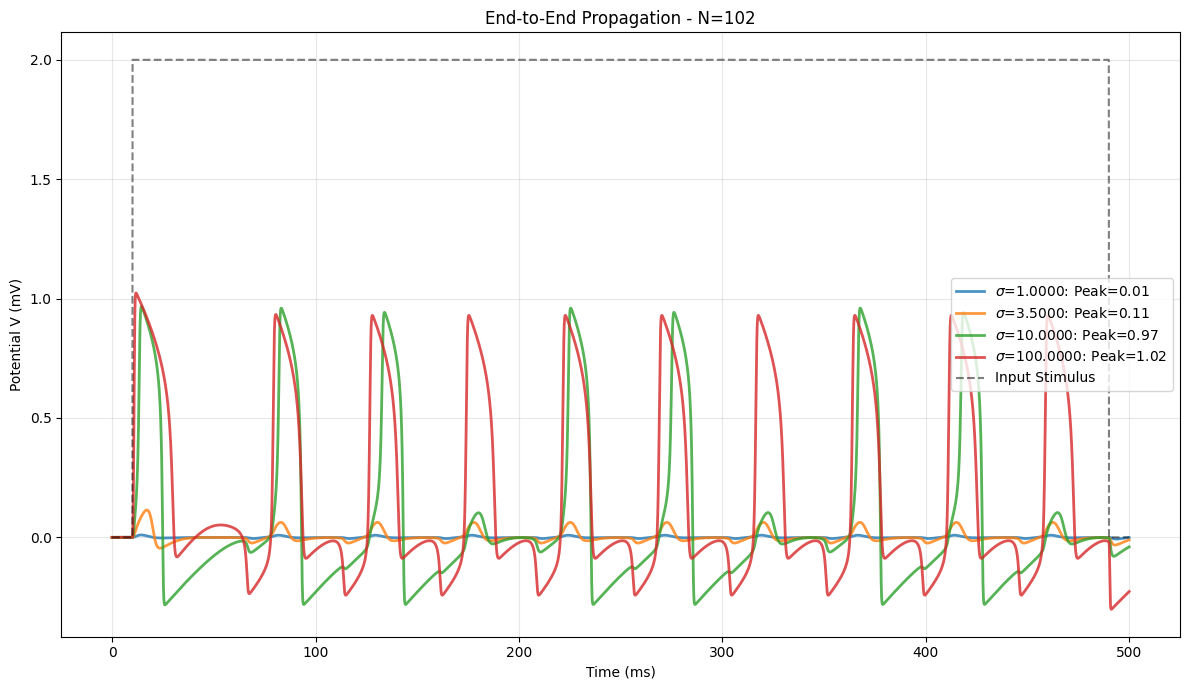
\includegraphics[width=0.8\textwidth]{img/FH_model/BA_Network/diffusion_coeff_BA_N=100.png}
    \caption{Dynamical transition of the neural network as the diffusion coefficient $\sigma$ varies. For low values of $\sigma$, the signal fails to propagate efficiently, whereas a critical threshold allows for coherent signal transmission.}
    \label{fig:diffusion_transition}
\end{figure}

%Dovrei studiare qual è la critical treshold per cui il segnale passa?

This empirical observation is rigorously supported by the numerical study of the spectral gap of the network's directed Laplacian, specifically the first non-zero real part of the eigenvalues, $\text{Re}(\lambda_2)$. In networked dynamical systems, the global synchronization and the ability of a perturbation to travel across the graph without quenching are governed by the effective macroscopic diffusion rate, which is proportional to the product $\sigma \text{Re}(\lambda_2)$ \cite{barrat2008dynamical}. 

Although standard Erdős–Rényi (ER) and Barabási-Albert (BA) graphs typically exhibit a spectral gap that decays logarithmically as $\mathcal{O}((\ln N)^{-1})$ due to their small-world properties, the strict structural bottleneck introduced by our specific boundary conditions (forcing the flow through a single input node and a single output node) profoundly alters the transport topology. This boundary constraint effectively forces the energy flow into a quasi-one-dimensional transport regime. As a result, our numerical spectral analysis demonstrates that $\text{Re}(\lambda_2)$ collapses linearly, scaling exactly as $\mathcal{O}(N^{-1})$ for both the ER and BA setups.

\begin{figure}[htbp]
    \centering
    \begin{minipage}{0.49\textwidth}
        \centering
        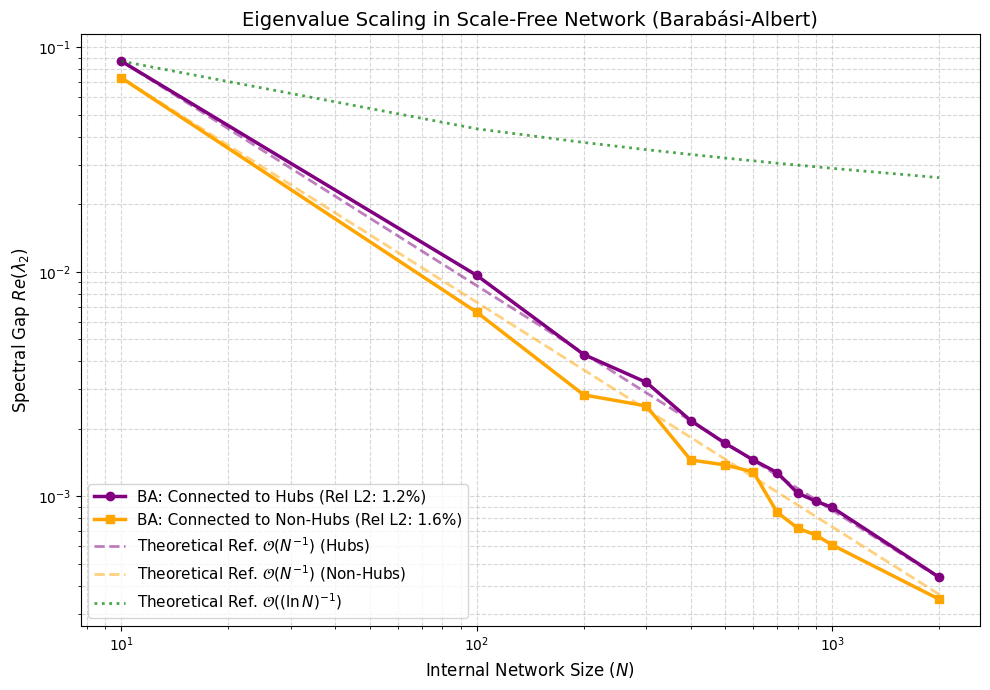
\includegraphics[width=\textwidth]{img/FH_model/BA_Network/Spectral_gap_BA.png}
        \caption{Scaling of the spectral gap $\text{Re}(\lambda_2)$ as a function of $N$ for the Barabási-Albert (BA) topology, showing the $\mathcal{O}(N^{-1})$ decay.}
        \label{fig:spectral_gap_ba}
    \end{minipage}\hfill
    \begin{minipage}{0.49\textwidth}
        \centering
        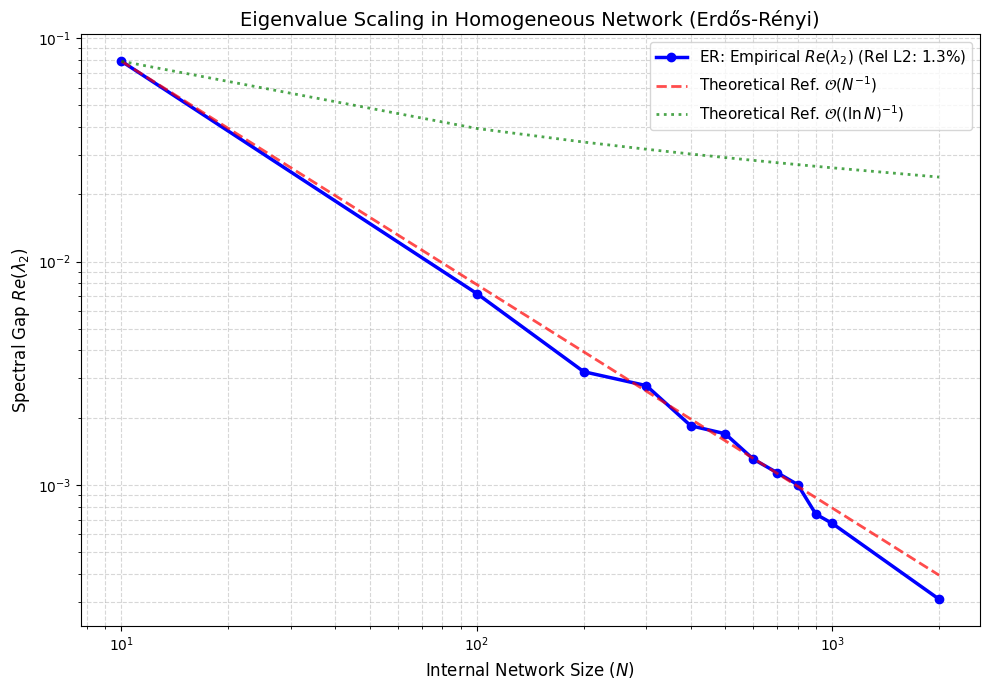
\includegraphics[width=\textwidth]{img/FH_model/ER_Network/Spectral_gap_ER.png}
        \caption{Scaling of the spectral gap $\text{Re}(\lambda_2)$ as a function of $N$ for the Erdős–Rényi (ER) topology, confirming the identical $\mathcal{O}(N^{-1})$ decay limit.}
        \label{fig:spectral_gap_er}
    \end{minipage}
\end{figure}

Therefore, to maintain a constant effective macroscopic coupling ($\sigma \text{Re}(\lambda_2) \approx \text{constant}$) and ensure that the operator learns a consistent continuous continuum limit regardless of the spatial discretization size $N$, the physical diffusion coefficient must systematically scale as $\sigma \propto N$.

%Let's focus on the case of the ER network. Here, since the connection probability is $p=\frac{3}{N}$ the average degree is fixed: $\lt k\gt = 3$.

For our experiments we chose $\sigma=0.1*N$.

%%%%%%%%%%%%%%%%%%%%%%%%%%%%%%%%%%%%%%%%
%REAL DATA
%%%%%%%%%%%%%%%%%%%%%%%%%%%%%%%%%%%%%%%%

\newpage
\section{Real data}
\subsection{The dataset}
After validating the Operator Learning approach on synthetic data generated by deterministic models (Hodgkin-Huxley and FitzHugh-Nagumo) and on complex networks, we now extend the analysis to real electrophysiological data.

The transition from the simulated to the biological domain introduces significant challenges. In synthetic models, the cause-and-effect relationship is well-defined: a known input current $I_{app}(t)$ produces a deterministic (or stochastic with controlled noise) voltage response. 

In real experimental data, however, the observed neuronal response is the result of the integration of multiple signals: not only the sensory stimulus controlled by the experimenter, but also feedback signals, the internal state of the animal, attention, preparatory motor activity, and intrinsic background noise. 

Consequently, the fundamental assumption of Operator Learning---namely, the existence of an operator $G: u \to v$ that uniquely maps a single input to the observed response---is a simplification. In this work, we will nevertheless assume this framework to be valid, treating the unobserved variables as stochastic noise that the neural network must filter out in order to learn the average dynamics induced by the stimulus.

%We now delve into the application of our machinery to a real neural system.
%In particular, we wanted to preserve the point of view of an emulation of an unknown underlying neural network.
The dataset employed in this work originates from the classic vibrotactile discrimination experiments conducted by Romo's group \cite{Romo_1999_Nature}.
The experiment consists of a working memory task performed by trained macaques. The protocol, termed \textit{two-alternative forced-choice} (2AFC), is structured into the following phases:
\begin{enumerate}
    \item \textbf{Stimulus 1 ($f_1$):} A probe vibrates on the monkey's fingertip at a frequency $f_1$ for 500 ms.
    \item \textbf{Delay:} A delay period (typically 3-6 seconds) during which no stimulus is presented. The monkey must maintain the memory trace of $f_1$.
    \item \textbf{Stimulus 2 ($f_2$):} A second vibration with frequency $f_2$ is presented for 500 ms.
    \item \textbf{Decision:} The monkey must indicate, by pressing one of two buttons, whether $f_2 > f_1$ or vice versa.
\end{enumerate}


\begin{figure}[htbp]
    \centering
    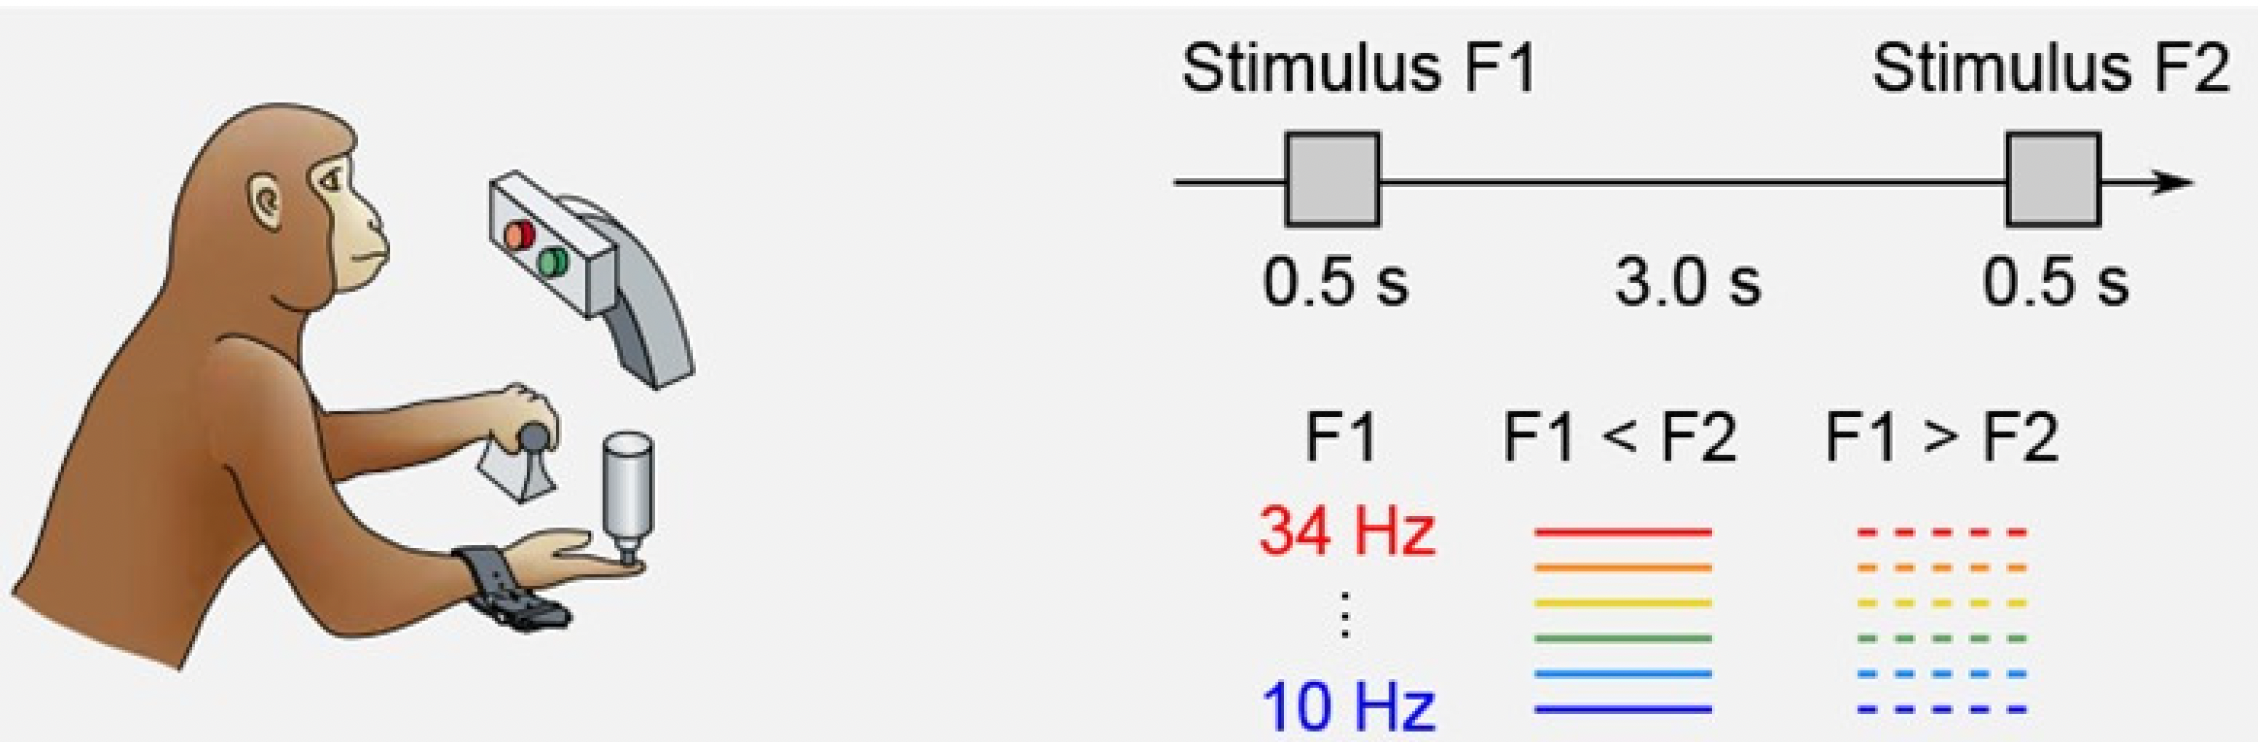
\includegraphics[width=0.85\textwidth]{img/Real_Data/Romo_task.png}
    \caption{Sequence of events in the vibrotactile two-alternative forced-choice (2AFC) task. The monkey perceives the first mechanical stimulus ($f_1$), maintains its trace in working memory during the delay period, and compares it against the second stimulus ($f_2$) to execute the motor decision.}
    \label{fig:romo_task}
\end{figure}

The possible choices for frequences $f_1$ and $f_2$ are {10,
14, 18, 26, 30, 34}.
Moreover, the data consist of extracellular recordings of individual neurons (Single Unit Activity) from the ventral prefrontal cortex (VPC), a crucial area for the maintenance of short-term memory and decision-making processes.

\subsection{First preprocessing}
The raw data consist of \textit{spike trains}, which are discrete temporal sequences indicating the exact moments a neuron generates an action potential. Since FNO (and in general Neural Operators) operate on continuous functions, a preprocessing step is required to transform these discrete events into continuous \textit{firing rates}.

The preprocessing involved the following steps:
\begin{enumerate}
    \item \textbf{Instantaneous Firing Rate Calculation:} The spike trains were convolved with a Gaussian kernel ($\sigma = 50$ ms) and sampled at $100$ Hz to obtain a continuous estimate of the firing probability density over time.
    \item \textbf{Time Warping and Alignment:} Since the duration of the experimental phases can vary slightly across trials, and the neuronal response can exhibit variable latencies, the data were temporally aligned (\textit{time-warped}) using a piecewise-linear transformation. Specifically, we defined key alignment events based on the task structure, such as the onset and offset of the first ($f_1$) and second ($f_2$) vibratory stimuli. Mathematically, let $t_i$ be the exact times of these specific events in a given trial, and $T_i$ be the median times of those same events computed across all trials. The instantaneous firing rate $x(t)$ was stretched or compressed along the time axis such that each trial-specific event $t_i$ was mapped precisely to the global median time $T_i$. This guarantees that the stimulus phases coincide perfectly across all samples, which is a crucial requirement to allow the neural network to learn consistent temporal patterns.
    \item \textbf{Filtering and Normalization:} To stabilize the variance and avoid numerical artifacts, neurons with atypically high mean firing rates (above $50$ Hz) were excluded from the dataset. Finally, the data matrix was mean-centered by subtracting the overall mean firing rate from the individual neural responses before further analysis. Moreover, since the overall error rate was 6\%, we analyzed only correct trials. 
\end{enumerate}

Figure \ref{fig:preprocessing_rates} shows an example of the preprocessed firing rates for different trials. The high trial-to-trial variability ("noise") typical of \textit{in vivo} recordings is clearly noticeable (in particular a correlation between stimulus and output is hardly noticeable), making the direct learning of the single-neuron dynamics with respect to the stimulus a highly challenging task.

\begin{figure}[H]
    \centering
    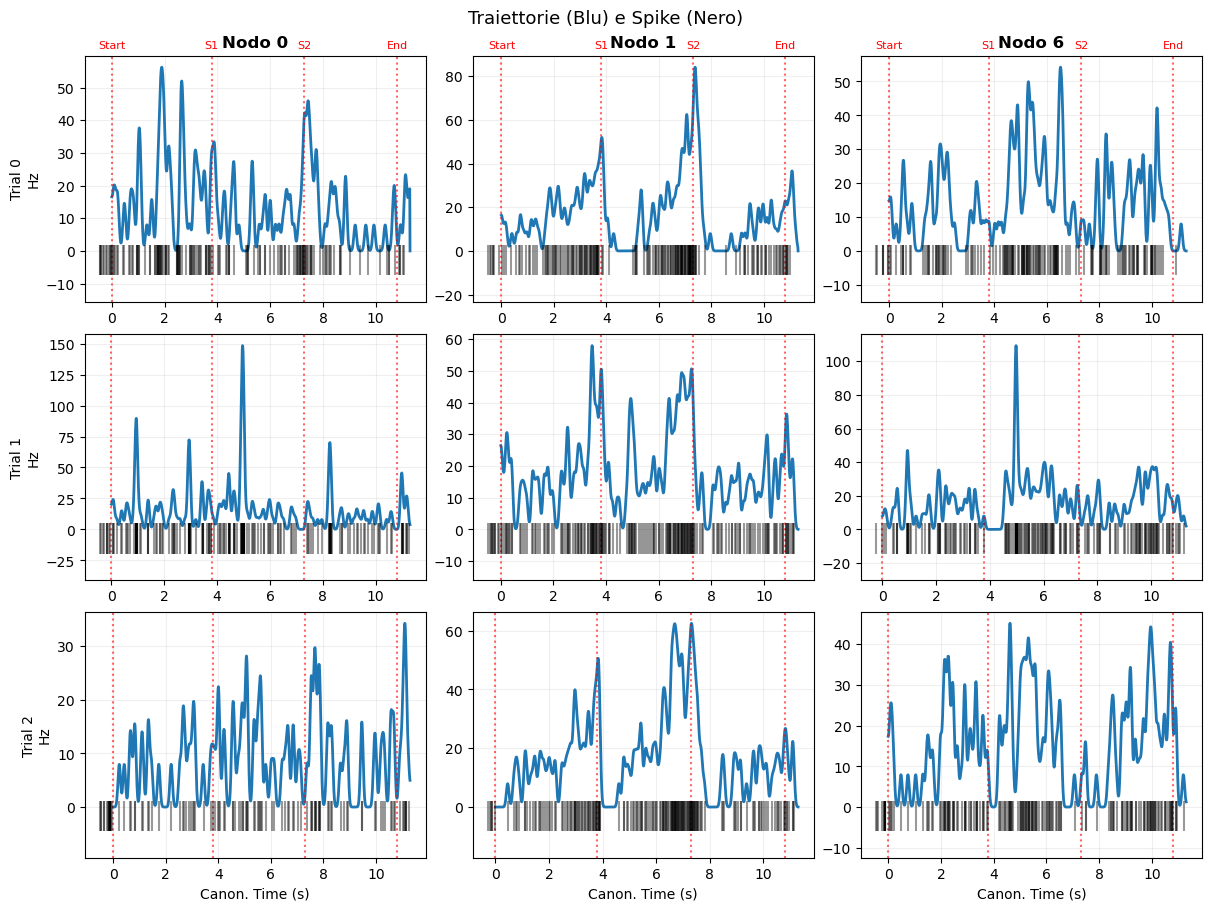
\includegraphics[width=0.8\textwidth]{img/Real_Data/Monkey_output_semi_raw.png}
    \caption{Example of preprocessed neuronal activity for a single neuron across multiple trials. The curves represent the \textit{warped firing rate}. Note the significant variability in the response even to the exact same stimulus, which is due to intrinsic noise and unobserved dynamics.}
    \label{fig:preprocessing_rates}
\end{figure}

\subsection{Second preprocessing: dPCA}
Given the noisy and high-dimensional nature of the population activity (hundreds of recorded neurons), training a neural operator on the single raw channels is highly ineffective. To extract the task-relevant latent dynamics, we applied \textbf{Demixed Principal Component Analysis (dPCA)} \cite{Kobak_2016_dPCA}.

Unlike standard PCA, which maximizes the total variance of the data without taking the experimental condition labels into account, dPCA decomposes the total variance into marginal components attributable to specific task parameters. In our case, given the neural activity tensor $\mathbf{X}$ (a multidimensional array containing the instantaneous firing rates of $N$ neurons across $S$ stimuli, $Q$ decisions, $K$ trials, and $T$ time points), the data variance is mathematically partitioned into five parts: condition-independent, stimulus-dependent, decision-dependent, stimulus-decision interaction, and trial-to-trial noise. 

dPCA seeks a transformation matrix that projects the data into a latent space where the meaningful components are "demixed", isolating:
\begin{itemize}
    \item \textbf{Condition-independent (Temporal) Component:} Captures the dynamics common to all trials, representing the general temporal evolution of the task irrespective of the condition.
    \item \textbf{Stimulus-dependent Component:} Captures the variations in neural activity that depend exclusively on the sensory stimulus (i.e., the values of the frequencies $f_1$ and $f_2$).
    \item \textbf{Decision-dependent Component:} Captures the variance related to the animal's choice or motor response.
    \item \textbf{Interaction Component:} Captures the variance arising from the non-linear interaction between the stimulus and the decision.
\end{itemize}

The trial-to-trial variability is treated mathematically as a \textbf{Noise} term in the variance decomposition, which the dPCA loss function is explicitly designed to penalize and filter out during the dimensionality reduction process.

Formally, the objective is to find a decoder matrix $\mathbf{D}$ and an encoder matrix $\mathbf{F}$ that minimize the reconstruction error evaluated on the data marginalizations \cite{Kobak_2016_dPCA}. For the implementation, we utilized the official library provided by the authors\footnote{Code available on GitHub: \url{https://github.com/machenslab/dPCA}}.

Mathematically, let $\mathbf{X}$ be the centered data matrix containing the single-trial instantaneous firing rates of all $N$ recorded neurons. The marginalization procedure decomposes this matrix into a sum of parameter-specific averages (the marginalizations) and a trial-to-trial noise term:
$$ \mathbf{X} = \sum_{\phi} \mathbf{X}_{\phi} + \mathbf{X}_{noise} $$
where $\phi$ iterates over the relevant task parameters (e.g., condition-independent time, stimulus, decision, and their interactions). Each term $\mathbf{X}_\phi$ captures the portion of the data variance exclusively attributable to that specific parameter.

The core objective of dPCA is to find a set of decoder matrices $\mathbf{D}_\phi$ and encoder matrices $\mathbf{F}_\phi$ for each marginalization $\phi$. The decoders linearly project the full neural activity $\mathbf{X}$ into a low-dimensional latent space, while the encoders map this latent representation back to reconstruct the parameter-specific target $\mathbf{X}_\phi$. These matrices are obtained by minimizing the following loss function:
$$ L = \sum_{\phi} L_{\phi} = \sum_{\phi} ||\mathbf{X}_{\phi} - \mathbf{F}_{\phi} \mathbf{D}_{\phi} \mathbf{X}||^{2} $$

In experimental scenarios with unbalanced data (e.g., varying number of trials per condition, aborted trials, or self-paced tasks), this formulation is adapted to operate on trial-averaged firing rates (PSTHs), denoted as $\tilde{\mathbf{X}}$. By introducing a regularization parameter $\mu$ to prevent overfitting and a noise covariance matrix $\tilde{\mathbf{C}}_{noise}$, the objective function for each component is adjusted to:
$$ L_{\phi} = ||\tilde{\mathbf{X}}_{\phi} - \mathbf{F}_{\phi} \mathbf{D}_{\phi} \tilde{\mathbf{X}}||^{2} + SQT ||\mathbf{F}_{\phi} \mathbf{D}_{\phi} \tilde{\mathbf{C}}_{noise}^{1/2}||^{2} + \mu ||\mathbf{F}_{\phi} \mathbf{D}_{\phi}||^{2} $$
where $S$, $Q$, and $T$ represent the number of stimuli, decisions, and time points, respectively. This optimization problem amounts to a Reduced-Rank Regression (RRR) and can be efficiently solved analytically via Singular Value Decomposition (SVD).

For the training of our Neural Operator, we specifically selected the projection of the test set onto the decoder axis $\mathbf{d}$ corresponding to the \textit{first stimulus component}. This provides a one-dimensional, continuous latent trajectory $u(t)$ that represents the "pure response" of the neural network to the vibrotactile stimulus, efficiently filtered from noise and non-pertinent dynamics.

\begin{figure}[htbp]
    \centering
    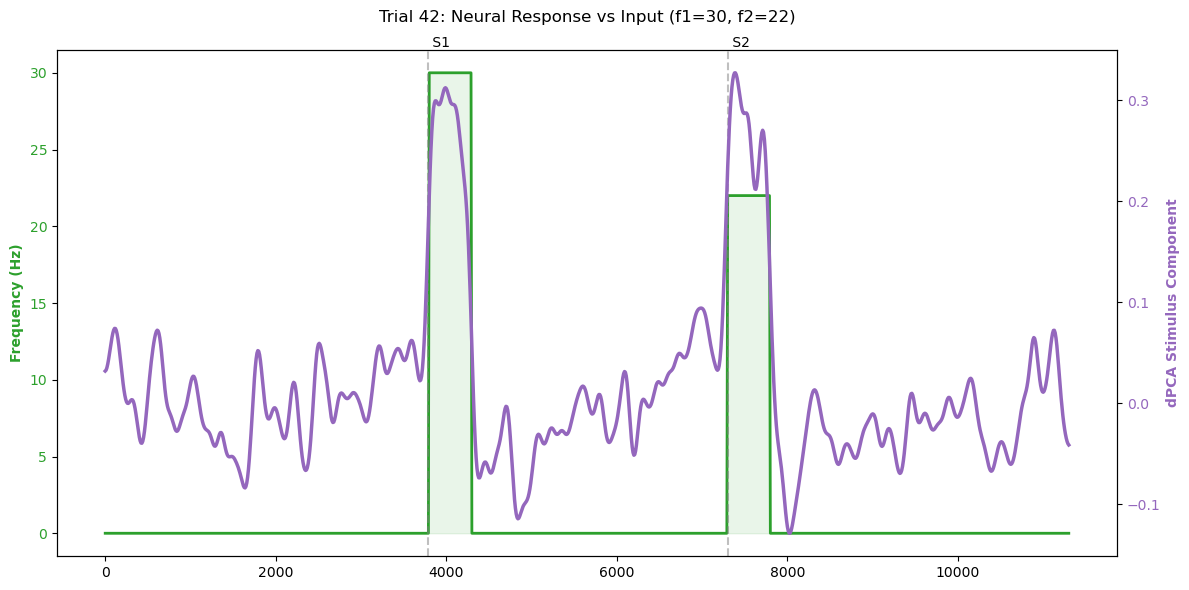
\includegraphics[width=\textwidth]{img/Real_Data/Monkey_dPCA.png}
    \caption{First stimulus dPCA component for an exemplary trial ($f_1 = 30$ Hz, $f_2 = 22$ Hz). The solid green line represents the applied stimulus frequency (left axis), while the solid purple line displays the corresponding projection of the population activity onto the first stimulus-dependent dPCA axis (right axis). Note how the latent neural trajectory reflects the stimulus presentation phases.}
    \label{fig:monkey_dpca_stimulus}
\end{figure}


\subsubsection{Comparison: PCA vs dPCA}

To better understand the advantage of dPCA, it is useful to compare it with standard Principal Component Analysis (PCA) and Linear Discriminant Analysis (LDA), as illustrated in Figure \ref{fig:pca_vs_dpca}.

Standard PCA is an unsupervised dimensionality reduction technique. It compresses the data by finding orthogonal axes (principal components) that maximize the explained variance and minimize the overall reconstruction error. However, because it is entirely blind to the experimental task parameters, the resulting components often exhibit mixed selectivity. Consequently, the temporal dynamics, stimulus information, and decision variables remain entangled within the same latent projections (Figure \ref{fig:pca_vs_dpca}c, d).

Conversely, LDA is a supervised method explicitly designed to find an axis that maximally separates different classes (e.g., different stimuli). While LDA perfectly demixes the task parameters, it does not attempt to preserve the original geometry of the data or minimize the reconstruction error, often leading to a distorted representation of the underlying neural population dynamics (Figure \ref{fig:pca_vs_dpca}a, b).

dPCA bridges the gap between these two approaches. By explicitly partitioning the data variance into marginalizations based on the task parameters (Figure \ref{fig:pca_vs_dpca}g), dPCA enforces a demixing constraint. Crucially, it gains additional flexibility by utilizing separate decoder and encoder matrices ($\mathbf{D}$ and $\mathbf{F}$). The decoder projects the data onto an axis that separates the task parameters (similar to LDA), while the encoder reconstructs the original class means, thereby preserving the structural geometry and minimizing the reconstruction error (similar to PCA) (Figure \ref{fig:pca_vs_dpca}e, f, h).

\begin{figure}[htbp]
    \centering
    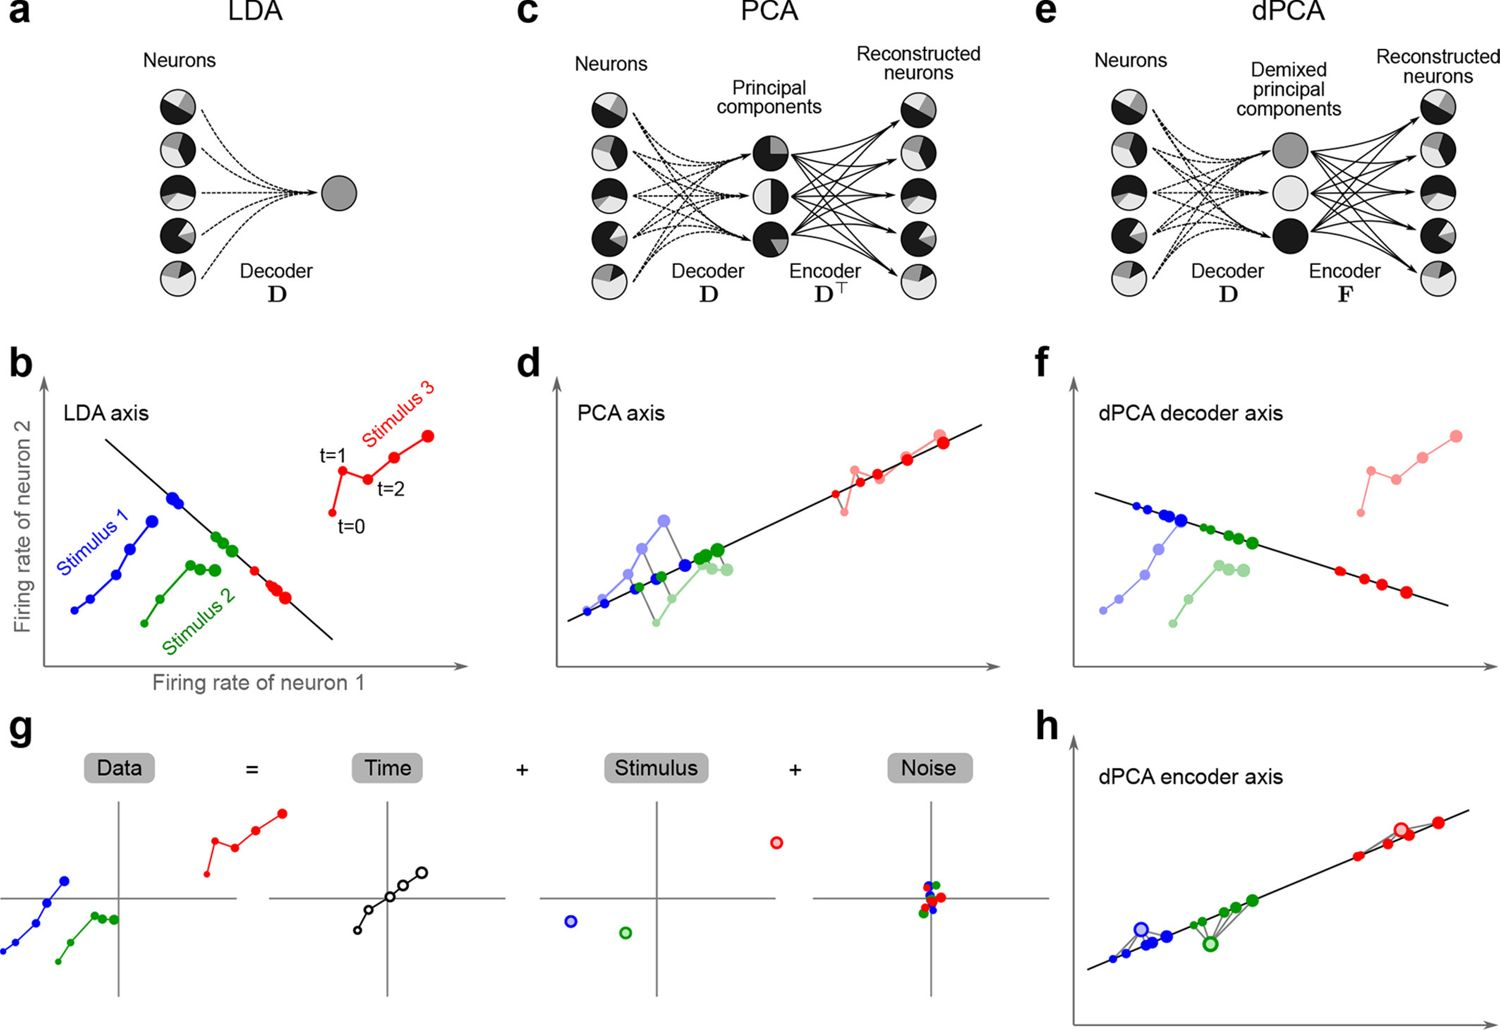
\includegraphics[width=\textwidth]{img/Real_Data/PCA vs dPCA.jpg}
    \caption{Comparison of Linear Discriminant Analysis (LDA), Principal Component Analysis (PCA), and demixed Principal Component Analysis (dPCA). (a, b) LDA separates the classes but distorts the geometric distances between them. (c, d) PCA accurately reconstructs the data and preserves distances but mixes the task parameters. (e-h) dPCA utilizes separate decoder and encoder matrices to effectively demix the task parameters while simultaneously preserving the original data geometry and minimizing reconstruction error.}
    \label{fig:pca_vs_dpca}
\end{figure}

\newpage
\subsection{Results with FNO}

In this section, we present the results of applying the Fourier Neural Operator (FNO) to learn the mapping from the sensory input to the latent neural dynamics. The input to the network was modeled as a simple square wave function: its amplitude represents the frequency of the applied vibrotactile stimulus, and its non-zero width corresponds to the true duration of the signal. The target output during training was the first stimulus-dependent latent trajectory extracted via dPCA, as described in the previous section.

Figure \ref{fig:fno_latent_results} illustrates the performance of the FNO in the latent space. Considering that the network is tasked with reproducing an entire, complex stimulus-driven neural dynamics from merely two macroscopic parameters (stimulus frequency and duration), the fits are remarkably accurate. The FNO successfully captures the transient peaks, the latency of the response, and the overall temporal evolution of the latent trajectory.

\begin{figure}[htbp]
    \centering
    \begin{subfigure}[b]{0.8\textwidth}
        \centering
        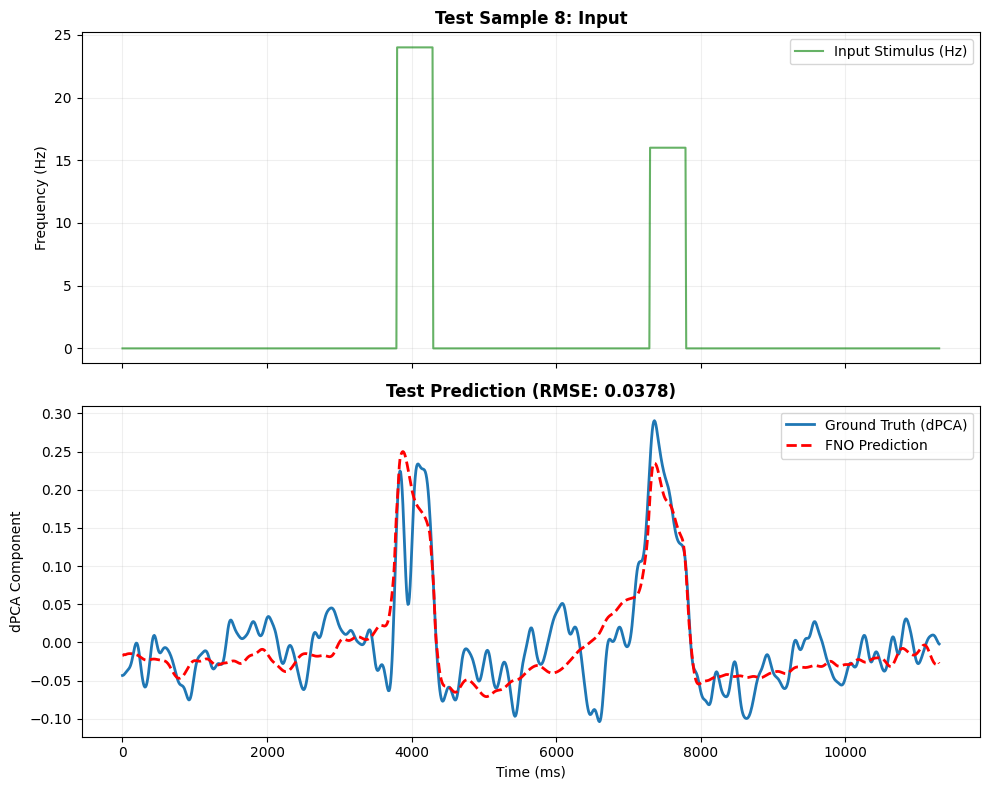
\includegraphics[width=\textwidth]{img/Real_Data/monkey_test_figure.png}
        \caption{Example of FNO prediction vs Ground Truth (1st stimulus dPC) for a test sample.}
    \end{subfigure}
    
    \vspace{0.4cm}
    
    \begin{subfigure}[b]{0.8\textwidth}
        \centering
        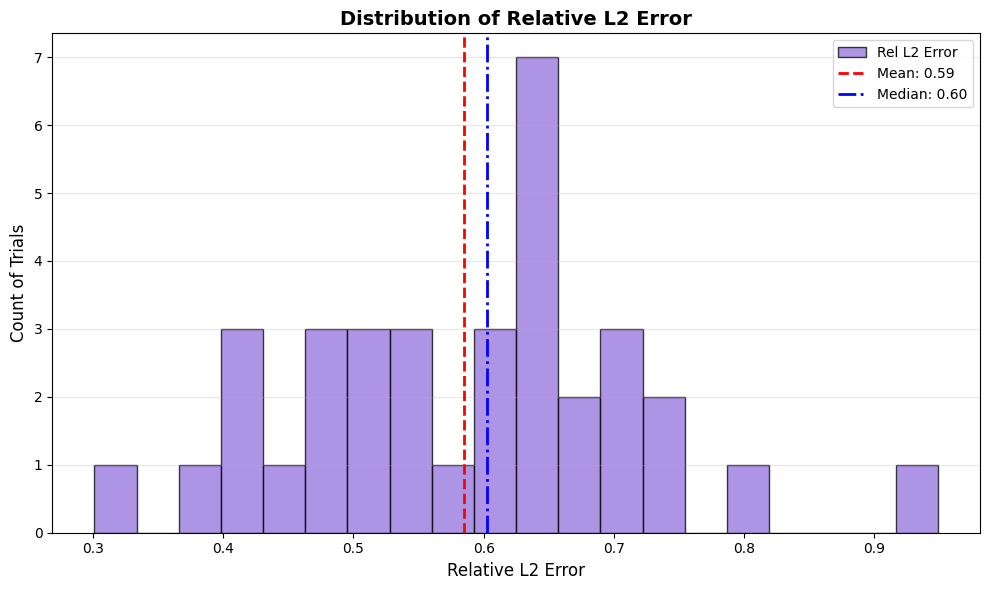
\includegraphics[width=\textwidth]{img/Real_Data/monkey_hist_test_set.png}
        \caption{Distribution of the relative $L_2$ error across the entire test set.}
    \end{subfigure}
    \caption{Performance of the FNO in predicting the latent stimulus dynamics.}
    \label{fig:fno_latent_results}
\end{figure}

To evaluate the predictive power of the model in the original physiological space, we performed the inverse transformation. This involved applying the inverse dPCA (multiplying the latent predictions by the corresponding encoder matrix $\mathbf{F}$) and subsequently reversing the time-warping procedure (de-warping) to restore the original trial timeframes. 

However, evaluating the model by reconstructing the total firing rate presents a visualization challenge. If we add back all the other marginalized components (such as the condition-independent baseline, decision, and interaction components) to our predicted stimulus component, the differences between the FNO prediction and the ground truth become virtually imperceptible. This occurs because the variance of the stimulus component is drastically smaller than the overall baseline and condition-independent activity (Figure \ref{fig:reprojection_total}). The stimulus-induced modulations are "masked" by the dominant task-general dynamics.

\begin{figure}[htbp]
    \centering
    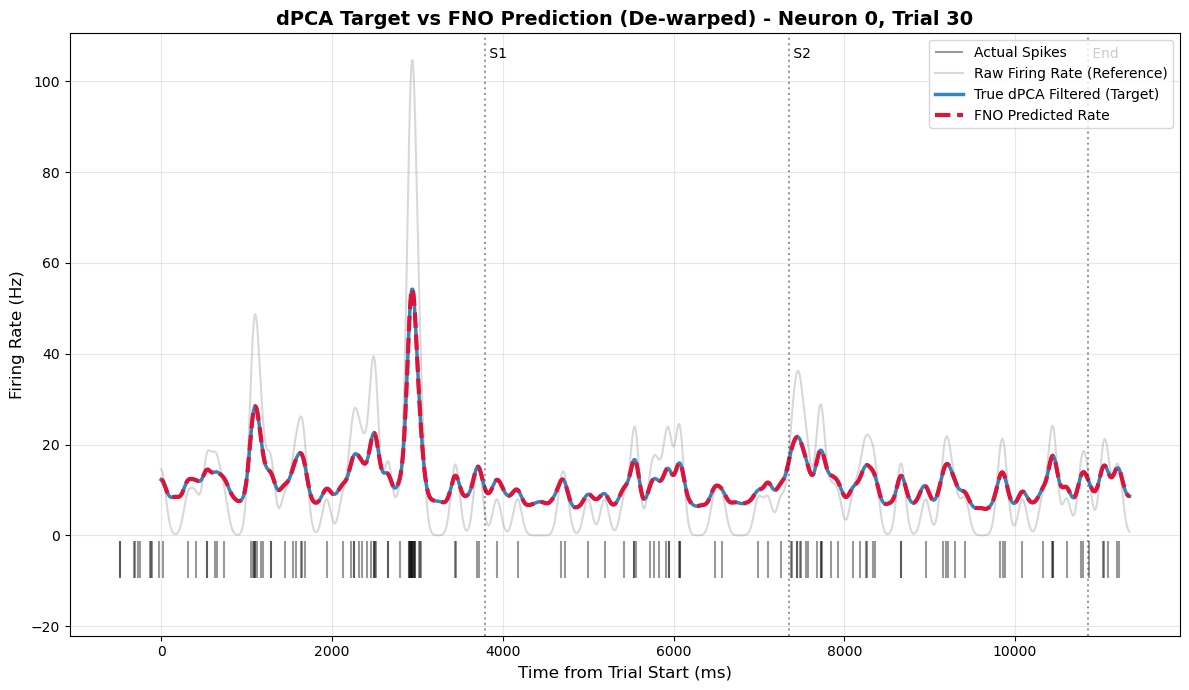
\includegraphics[width=0.9\textwidth]{img/Real_Data/Reprojection (total).png}
    \caption{Total reconstructed firing rate for a sample neuron (Neuron 0). When the predicted stimulus component is added back to the other task marginalizations, the overall predicted rate (dashed red line) almost perfectly overlaps the target (solid blue line), masking the specific contribution of the FNO due to the large scale of the condition-independent baseline.}
    \label{fig:reprojection_total}
\end{figure}

Therefore, a much more informative way to assess the FNO's performance in the direct space is to isolate and compare \textit{only} the pure stimulus component for individual neurons, ignoring the other marginalizations. 

Figure \ref{fig:reprojection_stimulus} shows this direct-space comparison for Neuron 8. This specific neuron was selected because it possesses the highest absolute weight in the encoder matrix corresponding to the first stimulus dPC. In biological terms, Neuron 8 is the unit within the recorded population that responds most strongly to the stimulus variations. The plot demonstrates that the FNO is highly capable of predicting the specific, real-space firing rate modulations induced by the vibrotactile stimuli, correctly locating the peaks corresponding to the $f_1$ and $f_2$ stimulation phases.

\begin{figure}[htbp]
    \centering
    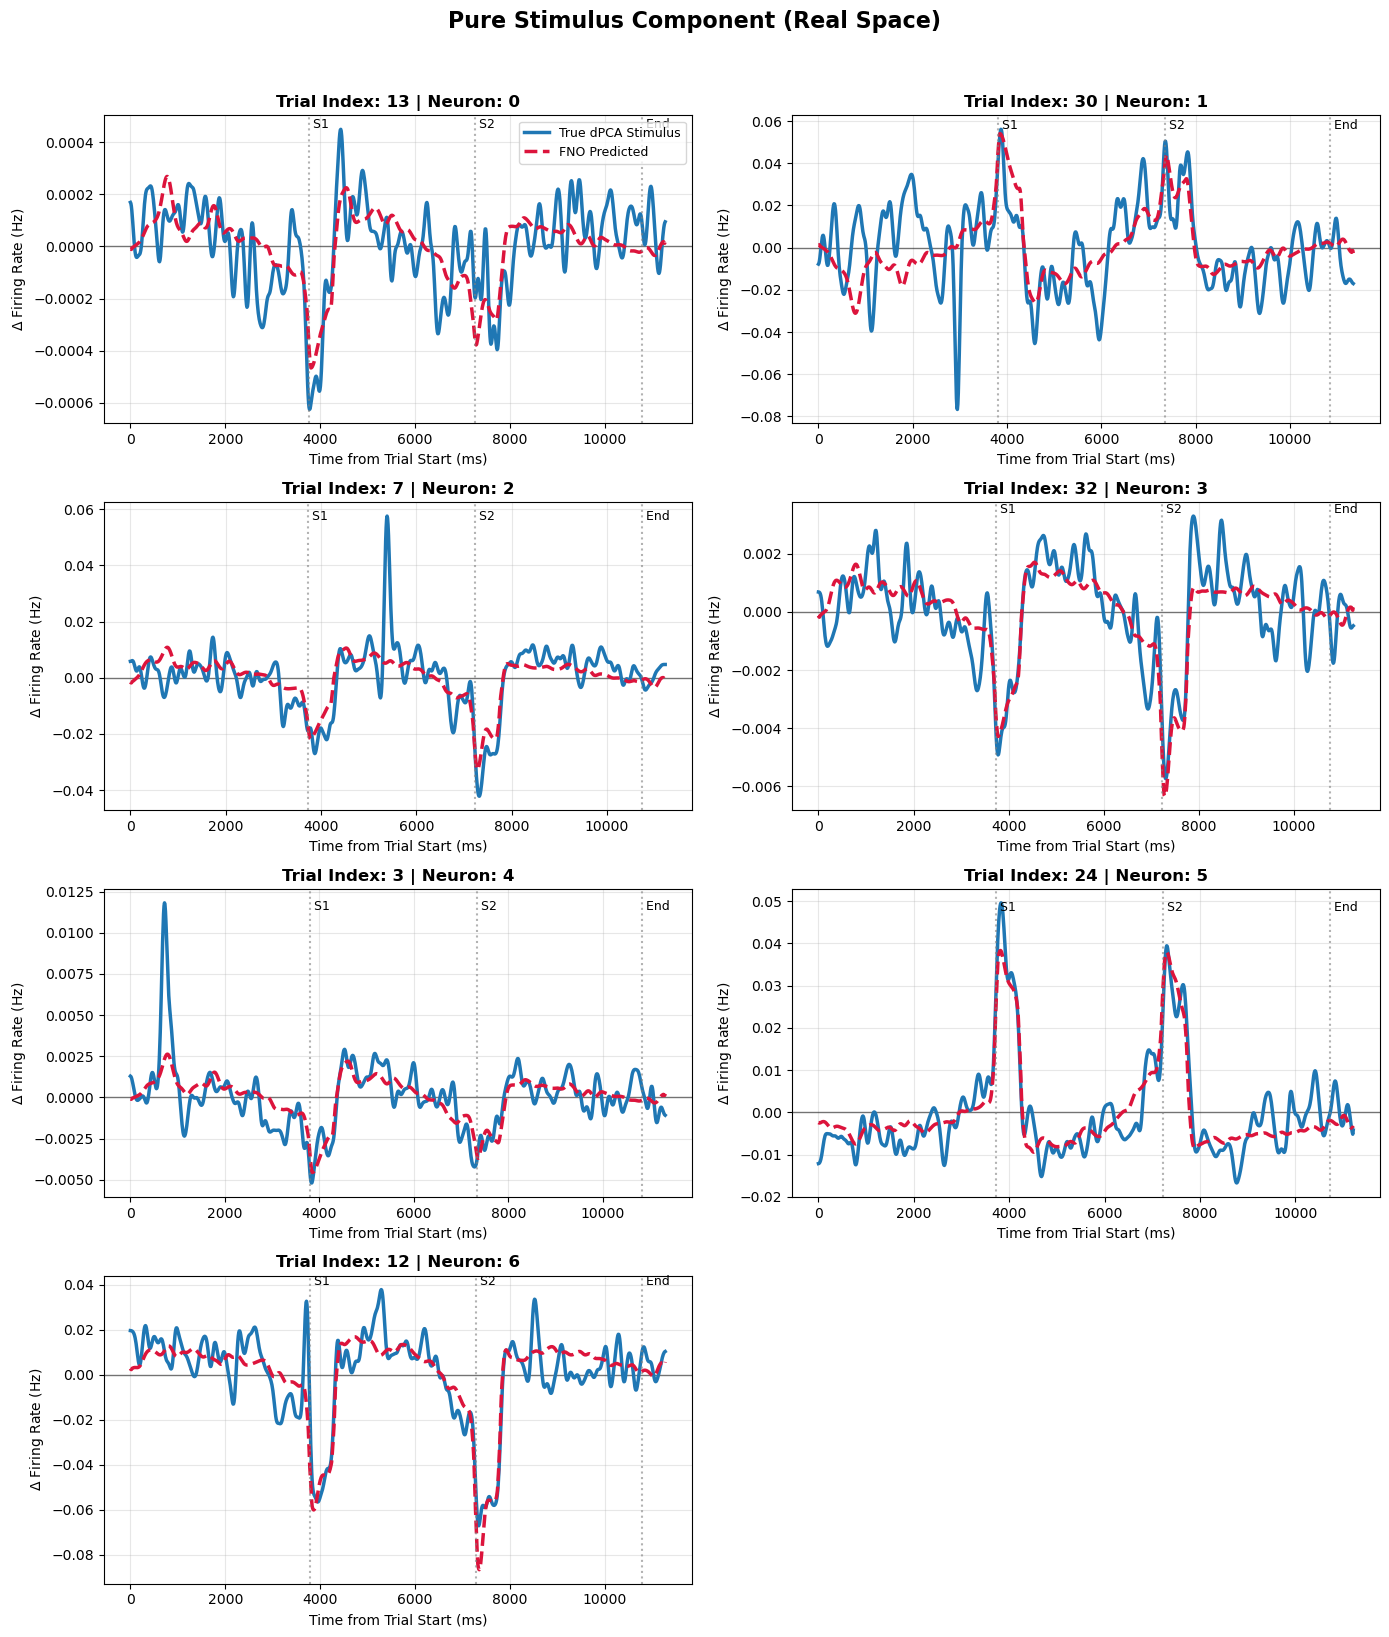
\includegraphics[width=0.9\textwidth]{img/Real_Data/Reprojection (stimulus) - multiple.png}
    \caption{Pure stimulus component in real space for Neuron 8 (the neuron with the highest encoder weight for the stimulus dPC). By isolating the stimulus effect from the overall baseline, we can clearly observe how well the FNO predicts the actual firing rate modulations during the $S_1$ and $S_2$ presentation windows.}
    \label{fig:reprojection_stimulus}
\end{figure}

\begin{table}[htbp]
\centering
\caption{dPCA Encoder weights for the first stimulus component ($f_1, f_2$). Neuron 1 exhibits the largest absolute weight, indicating the strongest firing rate modulation in response to the stimulus.}
\label{tab:encoder_weights}
\begin{tabular}{|l|c|}
\hline
\textbf{Neuron} & \textbf{Encoder Weight} \\ \hline
Neuron 0        & -0.0036                     \\
\textbf{Neuron 1} & \textbf{0.4141}           \\
Neuron 2        & -0.1695                     \\
Neuron 3        & -0.0273                     \\
Neuron 4        & -0.0349                     \\
Neuron 5        & 0.1287                      \\
Neuron 6        & -0.2490                     \\ \hline
\end{tabular}
\end{table}

 %   \input{chapters/demo-basic}
    % NOTE: I suggest to create a file for each chapter, like the previous \input{}.


    % --------------------------
    \part{\label{prt:Second section}Finding the Reaction Term in a Reaction-Diffusion System} % NOTE: dividing in parts is optional
    \chapter{Chapter 4}

In this final chapter we will first introduce reaction-diffusion equations in continuous and discrete domains. We will then present a hierarchy of progressively more sophisticated architectures to emulate such systems. We will test these architectures on a simple one dimensional system and on the FH two-dimensional model on a BA network. Finally, we will introduce a method to extract the phase diagram of the reaction potentials of these equations purely from data.

\section{Problem definition}
\subsection{Reaction-diffusion dynamics on complex networks}

Reaction-Diffusion (RD) systems constitute a cornerstone of mathematical physics, 
providing a fundamental framework to describe processes where the distribution of substances changes due to two competing mechanisms: 
local chemical reactions and spatial diffusion. Classically defined on continuous Euclidean domains $\Omega \subset \mathbb{R}^d$, 
these systems are governed by parabolic partial differential equations of the form:
\begin{equation}
    \frac{\partial \mathbf{u}}{\partial t} = \nu \Delta \mathbf{u} + \mathbf{f}(\mathbf{u}),
\end{equation}
where $\mathbf{u}(\mathbf{x},t)$ represents the state vector (e.g., chemical concentrations), $\nu$ is the diffusion coefficient, $\Delta = \nabla^2$ is the
Laplacian operator representing spatial diffusion, and $\mathbf{f}(\mathbf{u})$ describes the non-linear reaction kinetics. 
These dynamics are renowned for generating complex spatio-temporal patterns, such as Turing patterns, traveling waves, and spirals \cite{turing1952chemical,nakao2010turing}

Recent advances in Operator Learning have focused on learning these dynamics efficiently in continuous domains. Notably, Wang and Hao \cite{wang2025laplacian} proposed 
a \textit{Laplacian Eigenfunction-Based Neural Operator} (LE-NO). Their approach exploits the spectral decomposition of the continuous 
Laplacian to efficiently approximate the non-linear reaction term, demonstrating that spectral information is critical for learning accurate operators in 
reaction-diffusion problems.

However, many real-world complex systems—such as social networks, connectomes, and power grids—are 
intrinsically discrete and topologically irregular. On these \textit{Complex Networks}, 
the notion of continuous space is replaced by a graph topology $\mathcal{G} = (\mathcal{V}, \mathcal{E})$, consisting of $N$ nodes. Consequently, 
the continuous Laplacian operator is replaced by the \textbf{Graph Laplacian matrix} $\mathbf{L} \in \mathbb{R}^{N \times N}$, defined as:
\begin{equation}
    \mathbf{L} = \mathbf{D} - \mathbf{A},
\end{equation}
where $\mathbf{A}$ is the adjacency matrix and $\mathbf{D}$ is the diagonal degree matrix. The reaction-diffusion dynamics on the network are then governed by a system of coupled Ordinary Differential Equations (ODEs):
\begin{equation}
    \frac{d \mathbf{U}}{dt} = - \nu \mathbf{L} \mathbf{U} + \mathbf{F}(\mathbf{U}),
    \label{eq:react_diff_on_net}
\end{equation}
where $\mathbf{U}(t) \in \mathbb{R}^{N \times d_u}$ is the state of all nodes at time $t$. The term $- \mathbf{L} \mathbf{U}$ captures the diffusion process across the edges of the graph, driving the system towards consensus, while $\mathbf{F}(\mathbf{U})$ applies the non-linear reaction independently at each node.

While the spectral properties of $\mathbf{L}$ are well-studied in network science, the application of Operator Learning to predict these dynamics on complex graphs 
remains underexplored. 
The shift from the continuous paradigm to the discrete domain has diverse implications. For instance the advantage of Operator architectures becomes less clear, since we don't have anymore a continuous domain on which we can exploit the discretization-invariance property. However, we believe that this feature could be still useful when analyzing networks of varying sizes.
Specifically, the challenge lies in whether Neural Operators can effectively learn these dynamics "blindly" from nodal time-series, 
or if explicitly informing the network with the spectral geometry of $\mathbf{L}$ (via its eigendecomposition) provides a necessary inductive bias for generalization.

% Questo lo lascio alla fine come spunto futuro ?
Another interesting aspect, that is an original contibution of this thesis, is the possibility to derive a phase portrait from the distribution of $\mathbf{F}(\mathbf{U})$ learned by the neural network.

\section{Methodology}

\subsection{Problem formulation}
We consider a dynamical system defined on a graph $\mathcal{G} = (\mathcal{V}, \mathcal{E})$, whose state $\mathbf{u}(t) \in \mathbb{R}^N$ evolves
according to Eq. \eqref{eq:react_diff_on_net}. 
Our aim was to predict an approximation of the \textbf{time-stepper operator} $\Psi_{\Delta t}$, which maps the system state from time $t$ to time $t + \Delta t$.
%on an undirected, connected graph $\mathcal{G} = (\mathcal{V}, \mathcal{E})$ with $N = |\mathcal{V}|$ nodes. 
%The state $\mathbf{u}(t) \in \mathbb{R}^N$ evolves according to a semi-linear PDE discretized on the graph:


\subsubsection{Experimental design: hierarchy of inductive bias}
\label{sec:exp_design}
To systematically evaluate the impact of physical and topological information on learning performance, we compared three architectures with increasing levels of "inductive bias".

\subsubsection{Level 1: totally blind (black-box)}
This baseline represents the purely data-driven approach. The model ignores both the diffusion physics and the graph topology. It attempts to learn the discrete time-stepper operator $\Psi_{\Delta t}$ end-to-end:
\begin{equation}
    \mathbf{u}^{n+1} \approx \text{Net}_{\theta}(\mathbf{u}^n)
\end{equation}
Here, the network must implicitly learn both the diffusion operator $-\nu \mathbf{L}$ and the reaction operator $\mathbf{F}$ simultaneously from data. This implies that the network must statistically reconstruct the graph structure solely from the propagation of signals, a task that typically requires massive amounts of training data. Moreover, we decided, to compare the same families of architectures and further analyze the importance of using topological information for the prediction, to use continuous operator network, which required us to embed the graphs in a continuous spatial domains. This first level is the only approach which does not require topological information.

\subsubsection[Level 2: physics-informed (hybrid nodal)]{Level 2: Physics-Informed\footnote{We chose this name given the strong connection with the Physics Informed Neural Networks (PINNs) family.} (Hybrid Nodal)}
In this approach, we injected physical knowledge by using an \textbf{Implicit-Explicit (IMEX)} solver \footnote{see Appendix \ref{app:C}.}. We assume the linear diffusion term $-\nu \mathbf{L}$ is known, and the network is tasked \textit{only} with approximating the reaction term $\mathbf{F}(\mathbf{u})$.

The update rule enforces the diffusion physics exactly:
\begin{equation}
    (\mathbf{I} + \Delta t \nu \mathbf{L}) \mathbf{u}^{n+1} = \mathbf{u}^n + \Delta t \cdot \text{Net}_{\theta}(\mathbf{u}^n)
    \label{eq:imex_update}
\end{equation}
%While "Physics-Informed", this model remains \textbf{"Topologically Blind"} regarding the reaction learning: the network approximates $\mathbf{F}(\mathbf{u})$ node-wise using a normalized coordinate system, ignoring the graph's symmetries and spectral clusters.


%

%\newline 
While the diffusion coefficient $\nu$ can be treated as a known physical prior, it can also be discovered directly from observational data. In our experiments, we cast this as a joint system identification problem: $\nu$ is initialized as a differentiable scalar variable and optimized end-to-end alongside the neural network weights $\theta$ via gradient descent.
It is worth noting that the neural network $\text{Net}_{\theta}(\mathbf{u})$ remains \textbf{"topologically blind"}. As in Level 1, it relies on embedding the discrete graph into an artificial continuous domain. However, this limitation is less detrimental in this hybrid formulation: since the target reaction term is strictly local (acting node-wise), explicitly capturing the spatial relations between nodes becomes less critical for the network. Nevertheless, this architectural flaw will be fully addressed in Level 3.

\subsubsection{Level 3: topology-informed (hybrid spectral)}
Here the model leveraged both physical and topological priors.
The diffusion operator was enforced exactly via the IMEX scheme as in Level 2.

Although the "Physics-Informed" approach ensures that the linear diffusion process is efficiently resolved by the numerical solver, the neural network $\text{Net}_{\theta}$ responsible for learning the non-linear reaction remains fundamentally \textbf{"topologically blind"}. While the exact mathematical formulation of the reaction term $\mathbf{F}(\mathbf{U})$ is intrinsically local (acting node-wise), learning this operator from observational data poses a severely ill-posed inverse problem. The temporal snapshots $\mathbf{u}^n$ embed global spatial correlations generated by the continuous diffusion process, and numerical approximations of time-derivatives inevitably amplify high-frequency noise. If $\text{Net}_{\theta}$ relies on a standard node-wise Multilayer Perceptron (MLP) or conventional operator architectures (such as standard FFT-based Fourier Neural Operators or Euclidean DeepONets), it processes the state variables using arbitrary or grid-based coordinates. Consequently, it completely ignores the true connectivity, symmetries, and spectral clusters of the complex network, making the learning process susceptible to local noise and spatial overfitting. To robustly decouple the local reaction kinetics from the inherent noise, it is necessary to explicitly embed the topological information of the Graph Laplacian $\mathbf{L}$ directly into the neural architecture. By doing so, for instance by using Laplacian eigenvectors to define the spectral layer in a LFNO, or substituting the trunk network of a DeepONet with Laplacian eigenfunctions as proposed in continuous domains by Wang and Hao \cite{wang2025laplacian}, the learning process is projected onto the graph's intrinsic, low-dimensional spectral manifold. This topological injection acts as a powerful structural prior: it regularizes the optimization landscape, naturally filters out non-physical, topology-violating noise, and enables the model to accurately recover the underlying local kinetics from globally coupled observations.
%However, the neural network approximated the reaction term in the \textit{graph spectral domain}, utilizing the eigenbasis $\mathbf{\Phi}$ of the Graph Laplacian $\mathbf{L}$.

\begin{comment}
One of our proposed methods, the \textbf{Laplacian Eigenfunction Neural Operator (LENO) on Network}, incorporates both physical and topological priors.
It operates in a \textit{truncated} spectral domain defined by the eigenvectors of the Laplacian.
Specifically, we select the matrix $\mathbf{\Phi}_p \in \mathbb{R}^{N \times p}$ containing only the eigenvectors corresponding to the $p$ smallest eigenvalues $0 \le \lambda_1 \le \dots \le \lambda_p$ (low-frequency modes), where $p < N$ is a hyperparameter chosen during training.

\begin{enumerate}
    \item \textbf{Projection:} Inputs are projected to low-dimensional spectral coefficients $\boldsymbol{\beta}^n = \mathbf{\Phi}_p^T \mathbf{u}^n \in \mathbb{R}^p$.
    \item \textbf{Learning:} A Network predicts the spectral residual of the reaction term: $\hat{\mathbf{R}} = \text{Net}_{\theta}(\boldsymbol{\beta}^n)$.
    \item \textbf{Update:} The next state is computed via the exact spectral IMEX scheme for the first $p$ modes:
    \begin{equation}
        \beta_k^{n+1} = \frac{\beta_k^n + \Delta t \hat{R}_k}{1 + \Delta t \nu \lambda_k}, \quad k=1,\dots,p
    \end{equation}
    The physical state is finally reconstructed as $\mathbf{u}^{n+1} \approx \mathbf{\Phi}_p \boldsymbol{\beta}^{n+1}$.
\end{enumerate}
%This model is \textbf{"Fully Informed"}: it leverages the exact solver for diffusion and the truncated native eigenbasis of the graph for efficient representation.
It is important to note that, since we posed the problem in the right coordinates, usually a simple MLP suffices to learn the coupling between modes, 
without the need for complex architectures (as we will see in the next section).
\end{comment}


\subsection{Training objective: composite loss strategy}
For the informed architectures (Levels 2 and 3), the learning task has been reframed: instead of predicting the state evolution directly, the networks approximated the non-linear reaction term $\mathbf{F}(\mathbf{u})$. To ensure both temporal stability and physical consistency, we employed a composite loss function consisting of two terms:
 a \textbf{Trajectory Loss} and a \textbf{Physics (Residual) Loss}.


\subsection{Ground truth reaction extraction}
Since the dataset contains state snapshots $\mathbf{u}$ but not explicit values for the reaction $\mathbf{F}(\mathbf{u})$, we first extracted the "ground truth" reaction target, denoted as $\mathbf{R}_{GT}$, by inverting the numerical scheme used for data generation.
Given the IMEX structure, the effective reaction responsible for the transition $\mathbf{u}^n \to \mathbf{u}^{n+1}$ is:
\begin{equation}
    \mathbf{R(u)}_{GT}^n = \underbrace{\frac{\mathbf{u}^{n+1} - \mathbf{u}^n}{\Delta t}}_{\text{Finite Difference}} + \underbrace{\nu \mathbf{L} \mathbf{u}^{n+1}}_{\text{Implicit Diffusion}}
\end{equation}
For Level 3, the target was the approximation $\mathbf{{R}_{GT}}^{n}_{p} = \mathbf{\Phi}_p^T \mathbf{R}_{GT}^n \mathbf{\Phi}_p$, or the projection onto the spectral domain: ${\hat{\mathbf{R}}_{GT}}^{n}_{p} = \mathbf{\Phi}_p^T \mathbf{R}_{GT}^n$, where the matrix $\mathbf{\Phi}_p \in \mathbb{R}^{N \times p}$ contains only the eigenvectors corresponding to the $p$ smallest eigenvalues $0 \le \lambda_1 \le \dots \le \lambda_p$ (low-frequency modes).

\subsubsection{Loss components}
The total loss $\mathcal{L}$ was defined as a weighted sum:
\begin{equation}
    \mathcal{L} = \mathcal{L}_{traj} + \lambda_{phys} \mathcal{L}_{phys}
\end{equation}
where $\lambda_{phys}$ is a balancing hyperparameter \footnote{in our experiments, we tuned $\lambda_{phys}$ as an hyperparameter of the model, before training.}
\footnote{For the blind architectures we used only the trajectory loss.}.

\begin{enumerate}
    \item \textbf{Physics (residual) loss ($\mathcal{L}_{phys}$):} 
    This term provided instantaneous supervision, forcing the neural network $\text{Net}_\theta$ to learn the local physical law governing the reaction.
\begin{equation}
    \mathcal{L}_{phys} = \frac{1}{N_{res}} \sum_{j=1}^{N_{res}} \| \text{Net}_\theta(\mathbf{x}_j) - \mathbf{R}_{GT}(\mathbf{x}_j) \|_2
\end{equation}
where $\mathbf{x}_j = \mathbf{u}_j^{m\left( j \right)}$ represents a single state snapshot for the $j$-th sample at a randomly sampled time step $m$ (different for each $j$) and $N_{res}$ is the batch size for the physical loss. Inputs $\mathbf{x}$ and targets $\mathbf{R}$ can be in nodal space or in spectral space (only for LENO).
\newline
    It is worth noting that this term acted analogously to the PDE residual loss ($\mathcal{L}_{PDE}$) found in classical Physics-Informed Neural Networks (PINNs), as it penalizes deviations from the governing equation.
    \footnote{However, unlike standard PINNs where the entire PDE is enforced via optimization (soft constraint), our hybrid framework enforced the diffusion
     operator exactly via the numerical architecture (hard constraint), leaving the loss function responsible solely for the reaction dynamics.}

\item \textbf{Relative trajectory loss ($\mathcal{L}_{traj}$):}
This term measured the relative error of the integrated next-step state. Normalizing by the ground truth magnitude ensured the loss is scale-invariant and prevented the model from biasing towards high-amplitude regions.
\begin{equation}
    \mathcal{L}_{traj} = \frac{1}{N_{traj} N_T} \sum_{i=1}^{N_{traj}} \sum_{n=0}^{N_T-1} \frac{\| \Psi_{\Delta t}(\hat{\mathbf{u}}^n_i, \theta) - \mathbf{u}^{n+1}_{true, i} \|_2}{\| \mathbf{u}^{n+1}_{true, i} \|_2 + \epsilon}
\end{equation}
where $\Psi_{\Delta t}$ represents the differentiable IMEX solver layer, $\hat{\mathbf{u}}^n_i$ is the predicted state at step $n$ (with $\hat{\mathbf{u}}^0_i = \mathbf{u}^0_{true, i}$), $\epsilon=10^{-6}$ is a small constant for numerical stability, $N_{traj}$ is the batch size for the trajectory, and $N_T$ is the total number of time steps.

    For the trajectory term we considered the relative L2 term for scale-invariance and better interpretability. However, during training, 
    we found that using the absolute L2 norm for the physics term provided better convergence properties \footnote{This particular choice depends on the specific problem. In section \ref{sec:Example 2} we used the relative loss also for the physics term.}.
\end{enumerate}



\subsection{Neural architectures implementation}

We instantiated the hierarchy of inductive biases defined in Sec. \ref{sec:exp_design} using the following specific architectures. All models were implemented in PyTorch.

\begin{itemize}
    \item \textbf{Level 1: black-box baselines.} (see Chapter \ref{Chp:2}) %Devo ancora creare la sezione di introduzione su ML e Neural Operators
    \begin{itemize}
        \item \textbf{Blind DeepONet:} In this baseline implementation, a \textit{Branch Net} (MLP) encoded the full global state vector, while a \textit{Trunk Net} (MLP) evaluated spatial basis functions at normalized coordinates $y \in [0,1]$. Crucially, these coordinates were assigned based solely on the node's arbitrary position within the 1D input data array (effectively mapping the $i$-th node in the dataset to the spatial coordinate $i/N$). By computing the final prediction through the dot product of these latent features, the architecture forced the discrete complex network onto a continuous 1D Euclidean domain. Consequently, it treated the graph nodes as uniformly spaced points on a line, restricting their spatial proximity to their arbitrary data storage order rather than their true topological connectivity.
        \item \textbf{Blind FNO:} A standard Fourier Neural Operator relying on the Fast Fourier Transform (FFT).
        Since the standard FFT cannot operate directly on non-Euclidean graph domains, the baseline FNO treated the node features as a flattened 1D sequence. This implicitly forced the network onto a uniformly spaced closed loop, where nodes are artificially connected based solely on their arbitrary array indices, completely ignoring the true graph topology.
         We truncated the frequency modes passed.
    \end{itemize}


\item \textbf{Level 2: physics-informed (hybrid)}\\
This tier decoupled physical laws from topological structure. Both architectures leveraged the \textbf{exact Graph-Spectral IMEX solver} for time-stepping, ensuring perfect diffusion dynamics via the true Graph Laplacian eigenvalues. However, the neural networks approximating the reaction term $\mathcal{N}(u)$ remained \textbf{topologically blind}, treating the graph signal as an Euclidean sequence.
\begin{itemize}
    \item \textbf{PI-DeepONet:} Utilized the standard Branch/Trunk architecture (same architecture as in level 1) to map the full state vector to the reaction residual.
    % It acted node-wise without explicit neighborhood information.
    \item \textbf{PI-FNO:} Used the FNO backbone (same architecture as in level 1) to predict the reaction vector. 
\end{itemize}

    \item \textbf{Level 3: topology-informed (spectral).}
    \begin{itemize}
        \item \textbf{Laplacian Eigenfunction Neural Operator (LENO) on network:} 
        This method operated in a \textit{truncated} spectral domain defined by the eigenvectors of the Laplacian.
Specifically, we selected the matrix $\mathbf{\Phi}_p \in \mathbb{R}^{N \times p}$ containing only the eigenvectors corresponding to the $p$ smallest eigenvalues $0 \le \lambda_1 \le \dots \le \lambda_p$ (low-frequency modes), where $p < N$ is a hyperparameter chosen during training.

\begin{enumerate}
    \item \textbf{Projection:} Inputs were projected to low-dimensional spectral coefficients $\boldsymbol{\beta}^n = \mathbf{\Phi}_p^T \mathbf{u}^n \in \mathbb{R}^p$.
    \item \textbf{Learning:} A Network predicted the spectral residual of the reaction term: $\hat{\mathbf{R}} = \text{Net}_{\theta}(\boldsymbol{\beta}^n)$.
    \item \textbf{Update:} The next state was computed via the exact spectral IMEX scheme for the first $p$ modes:
    \begin{equation}
        \beta_k^{n+1} = \frac{\beta_k^n + \Delta t \hat{R}_k}{1 + \Delta t \nu \lambda_k}, \quad k=1,\dots,p
    \end{equation}
    The physical state was finally reconstructed as $\mathbf{u}^{n+1} \approx \mathbf{\Phi}_p \boldsymbol{\beta}^{n+1}$.
\end{enumerate}
%This model is \textbf{"Fully Informed"}: it leverages the exact solver for diffusion and the truncated native eigenbasis of the graph for efficient representation.
It is important to note that, since we posed the problem in the right coordinates, usually a simple MLP suffices to learn the coupling between modes, 
without the need for complex architectures.

    \item \textbf{Graph (Laplacian)-FNO (ours):} It operated in a similar way to LENO.
    However it built on the standard FNO, so it replaced FFT/IFFT operations with the Graph Fourier Transform (GFT, where the input is projected onto the first $p$ eigenvectors of the Graph Laplacian ($\mathbf{\Phi}_p$)).
    
   The primary distinction between LFNO and LENO lies in the domain where the objective function is evaluated. While LENO minimizes the error directly on the transformed spectral coefficients, LFNO projects the latent representation back into the physical space via the inverse GFT, penalizing the reaction term directly at the nodal level.
    
        
        
%The proposed spectral residual learner. 
%Unlike deep FNOs, the core reaction approximation is handled by a concise MLP operating directly on the spectral coefficients $\boldsymbol{\beta}$, 
%leveraging the exact IMEX solver for the diffusion update.
    \end{itemize}
\end{itemize}

%\paragraph{Implementation Note.} 
%A key distinction from classical PINNs lies in constraint enforcement. While PINNs minimize the PDE residual as a soft loss term ($\mathcal{L}_{PDE}$), our Level 3 framework enforces the diffusion operator exactly via the numerical architecture (hard constraint) as shown in Eq. (\ref{eq:imex_update}). This strictly reduces the hypothesis space to physically valid diffusion processes on the graph.

%%%%%%%%%%%
\subsection{Training details}
All models were implemented in PyTorch and trained on an NVIDIA Quadro RTX 5000 GPU. To ensure reproducibility, fixed random seeds ($42$) were used for all experiments.

The network parameters were optimized using the Adam algorithm with a weight decay of $10^{-4}$ and a gradient clipping threshold of $1.0$ to ensure numerical stability
\footnote{Only for levels $2\&3$, since the loss can be more prone to stiffness and exploding gradients due to the inclusion of physical constraints and solver dynamics.}.
% We employed a mini-batch strategy with a batch size of $128$ for the trajectory data.

To select the optimal configuration, we performed an automated hyperparameter search using the \textit{Optuna} framework. To efficiently explore the search space, we utilized a \textit{Median Pruner} to early-stop unpromising trials. The search space included common parameters across all models and architecture-specific ones:
\begin{itemize}
    \item Learning rate: $\eta \in [10^{-5}, 5\cdot 10^{-3}]$ (log-uniform sampling);
    \item Physics penalty weight \footnote{Only for levels $2\&3$\label{fn:levels}}: $\lambda_{\text{phys}} \in [10^{-5}, 10.0]$ (log-uniform sampling);
    \item Initial guess for square root of the diffusion coefficient ($\nu= \varepsilon^2$)\textsuperscript{\ref{fn:levels}}: $\varepsilon_{\text{init}} \in [0.5, 2.0]$;
    \item Architecture-specific hyperparameters (e.g., hidden layer width, number of modes) were optimized within ranges appropriate for each specific model.
\end{itemize}

Once the best hyperparameters were identified, the final models were trained for $500$ epochs. The learning rate was scheduled to decrease by a factor of $\gamma = 0.5$ every $300$ epochs. 
To prevent overfitting, we monitored the error on a validation set and saved the model weights and fitted $\epsilon$, corresponding to the epoch with the lowest validation loss.

\section{Example 1: Allen-Cahn on graph (hierarchy of inductive bias)}

\subsection{Data generation}
To evaluate the proposed methods, we simulated the \textbf{Allen-Cahn equation} on a complex network. 
%The Allen-Cahn equation is a well-known reaction-diffusion model used in phase-transition problems.

%%%%%%%%%%%%%%%%%%%%%%%%%%%
The Allen-Cahn equation describes a reaction-diffusion process governed by the gradient flow of a Ginzburg-Landau free energy functional~\cite{allen1979microscopic}.
 While its primary application lies in predicting microstructural evolution during phase transitions in materials~\cite{chen2002phase},
  its ability to drive systems toward stable stationary states makes it a versatile tool. 
  Applications range from geometrical image segmentation~\cite{benes2004geometrical} to finding minimal cuts in graph theory and analyzing community structures
   in complex networks~\cite{bertozzi2012diffuse}.
%%%%%%%%%%%%%%%%%%%%%%%%%%%%
\subsection{Graph topology}
We generated a scale-free network using the \textbf{Barabási-Albert (BA)} model to mimic realistic topological features such as hubs and clusters.
\begin{itemize}
    \item \textbf{Nodes:} $N = 1000$.
    \item \textbf{Attachment:} $m = 2$ (each new node attaches to 2 existing nodes).
\end{itemize}

\subsection{Dynamics: Allen-Cahn on graphs}
The specific form of the reaction term for the Allen-Cahn equation is cubic:
\begin{equation}
    \mathbf{F}(\mathbf{u}) = \mathbf{u} - \mathbf{u}^3
\end{equation}
The system evolved from an initial condition of $50$, randomly selected, active nodes.
We generated a training dataset of $15000$ trajectories ($10000$ for training, $3000$ for validation and $2000$ for testing) by numerically integrating the system using 
a spectral IMEX solver \footnote{details in Appendix \ref{app:C}.},
 subsampling the snapshots at time intervals $\Delta=0.05 t$ for 21 time steps to create the input-target pairs. In Figure \ref{fig:experimental_design} we can observe the evolution of the node dynamics.

\begin{figure}
    \centering
    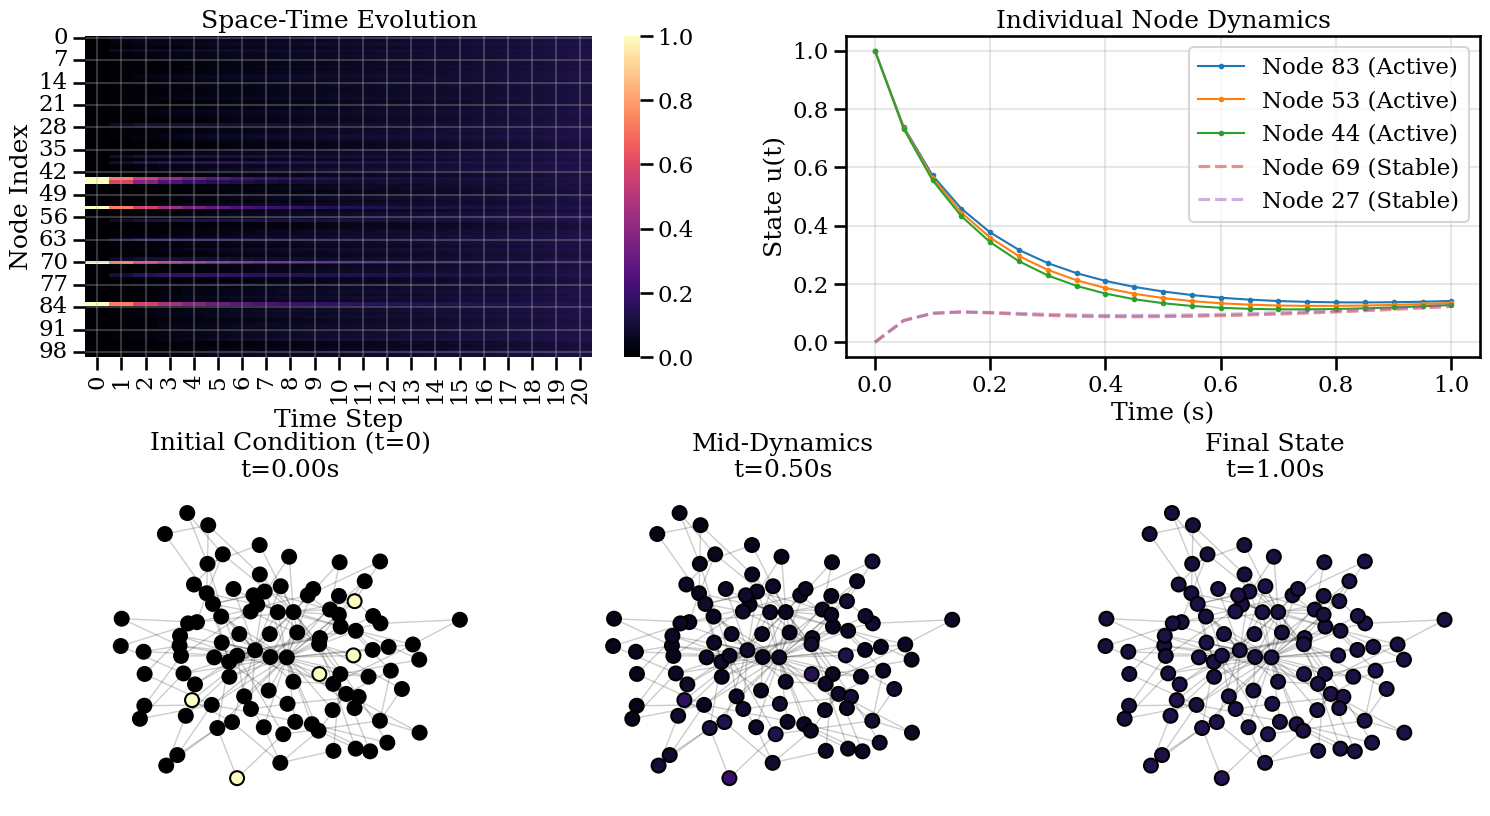
\includegraphics[width=1.0\textwidth]{img/Allen-Cahn/dynamics_Allen_Cahn_v2.png}
    \caption{Simulation of Allen-Cahn dynamics on a Barabási-Albert graph with $N=100$ nodes and $m=2$. The figure illustrates the evolution of all node states (top left, bottom) over time, and a focus on some representative nodes (top right), showcasing both the reaction and diffusive processes.}
    \label{fig:experimental_design}
\end{figure}

%%%%%%%%%

\subsection{Results and discussion}

\subsubsection{Quantitative analysis: error distribution}
We begin our analysis by examining the distribution of the relative $L_2$ errors on the test set (2000 trajectories). 
Figure \ref{fig:error_matrix} presents a systematic comparison of the test errors arranged by model family (columns) and inductive bias level (rows).
On the other hand Figure \ref{fig:heatmap_vertical_stack} shows an absolute error comparison between the same models, however it rearranges the two columns representing the families of architectures on the same page.

This visualization highlights the progressive improvement in generalization performance as we move from "Blind" models to "Topology-Informed" architectures.

%%%%%%%%%%%%%%%%%%%%%%%%%%%%%%
\begin{figure}[htbp]
    % Usiamo makebox per centrare la figura sforando i margini della pagina
    \makebox[\textwidth][c]{%
        % Aumenta o diminuisci 1.15 per gestire la grandezza totale (1.15 = 115% della larghezza del testo)
        \begin{minipage}{1.4\textwidth} 
            
            % --- HEADERS ---
            \begin{minipage}{0.05\textwidth} 
                \hfill 
            \end{minipage}
            \hfill 
            \begin{minipage}{0.46\textwidth} 
                \centering \textbf{DeepONet Family}
            \end{minipage}
            \hfill 
            \begin{minipage}{0.46\textwidth} 
                \centering \textbf{FNO Family}
            \end{minipage}
            \par\medskip

            % --- ROW 1: LEVEL 1 (BLIND) ---
            \begin{minipage}[c]{0.05\textwidth}
                \centering 
                \rotatebox{90}{\parbox{2.5cm}{\centering \textbf{Level 1} \\ (Blind)}}
            \end{minipage}
            \hfill
            \begin{minipage}[c]{0.46\textwidth}
                \centering
                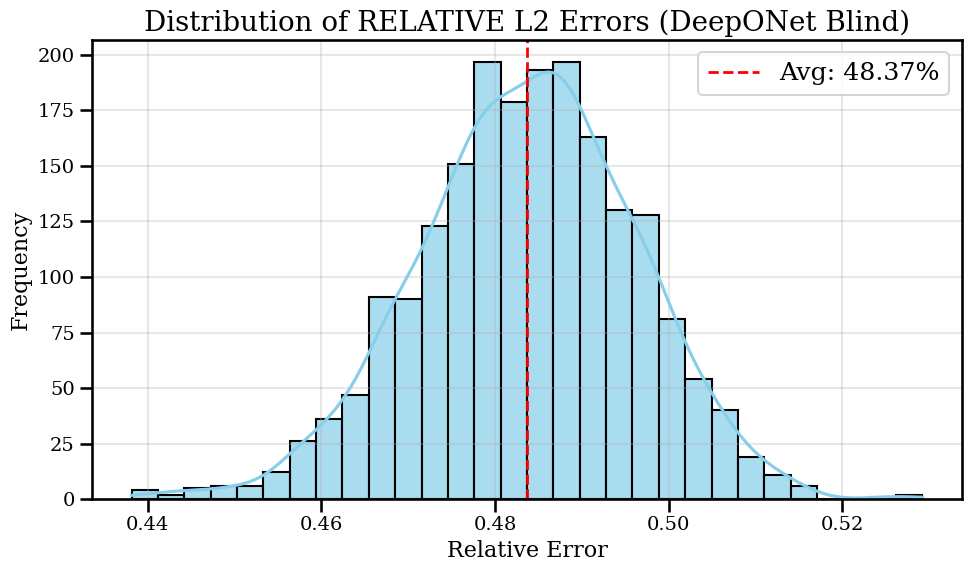
\includegraphics[width=\linewidth]{img/Allen-Cahn/Histograms/hist_test_set_deeponet_blind_v2.png}
            \end{minipage}
            \hfill
            \begin{minipage}[c]{0.46\textwidth}
                \centering
                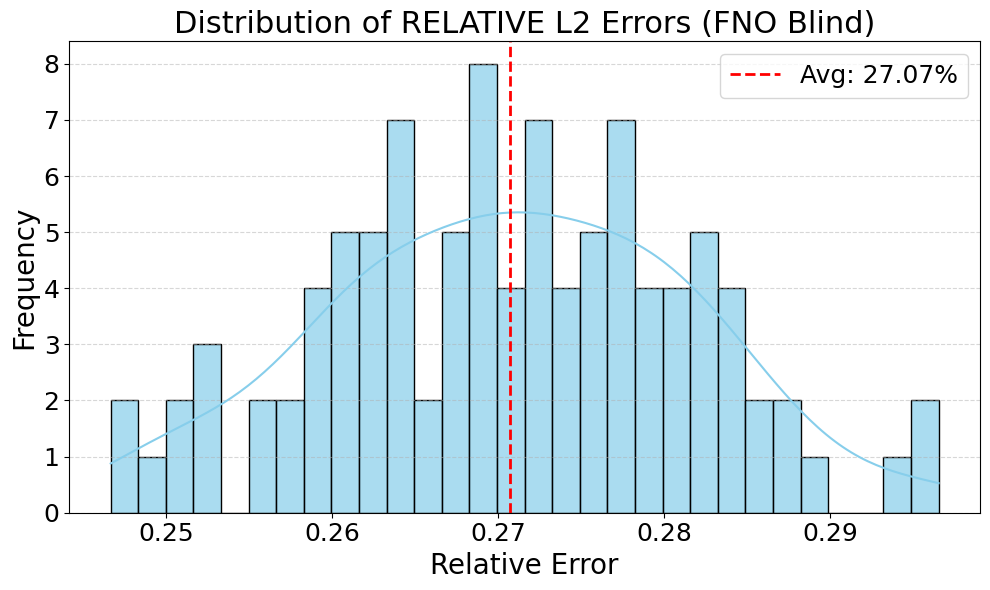
\includegraphics[width=\linewidth]{img/Allen-Cahn/Histograms/hist_test_set_FNO_blind_v2.png}
            \end{minipage}
            \par\bigskip 

            % --- ROW 2: LEVEL 2 (PHYSICS-INFORMED) ---
            \begin{minipage}[c]{0.05\textwidth}
                \centering 
                \rotatebox{90}{\parbox{2.5cm}{\centering \textbf{Level 2} \\ (Physics)}}
            \end{minipage}
            \hfill
            \begin{minipage}[c]{0.46\textwidth}
                \centering
                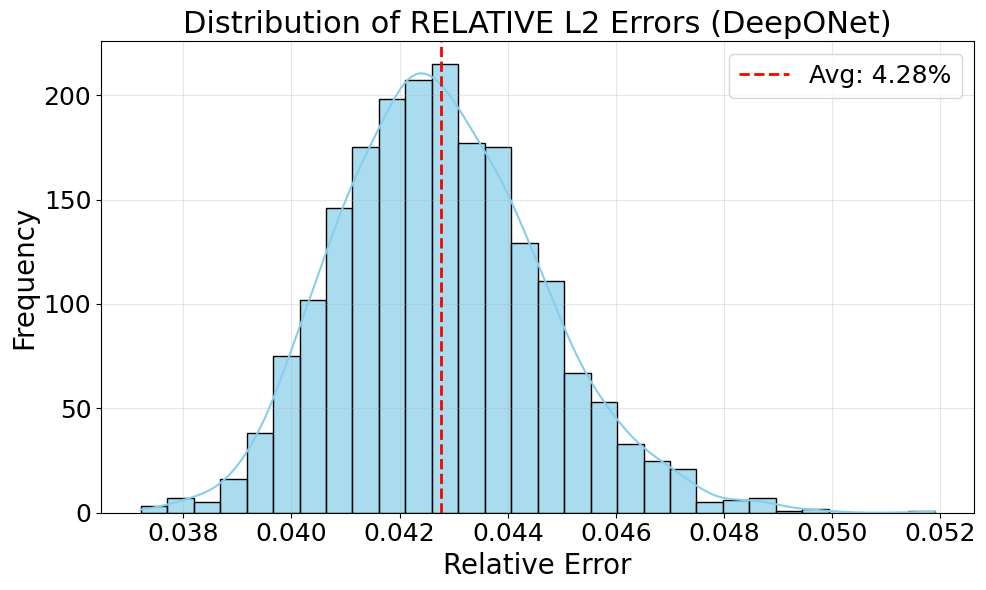
\includegraphics[width=\linewidth]{img/Allen-Cahn/Histograms/hist_test_set_deeponet_v2.png}
            \end{minipage}
            \hfill
            \begin{minipage}[c]{0.46\textwidth}
                \centering
                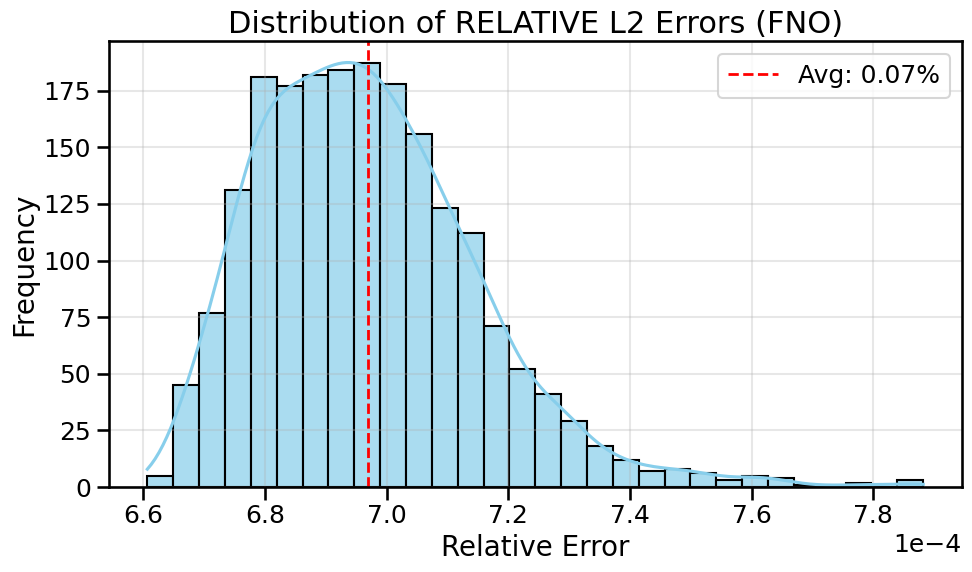
\includegraphics[width=\linewidth]{img/Allen-Cahn/Histograms/hist_test_set_FNO_v2.png}
            \end{minipage}
            \par\bigskip

            % --- ROW 3: LEVEL 3 (TOPOLOGY-INFORMED) ---
            \begin{minipage}[c]{0.05\textwidth}
                \centering 
                \rotatebox{90}{\parbox{2.5cm}{\centering \textbf{Level 3} \\ (Topology)}}
            \end{minipage}
            \hfill
            \begin{minipage}[c]{0.46\textwidth}
                \centering
                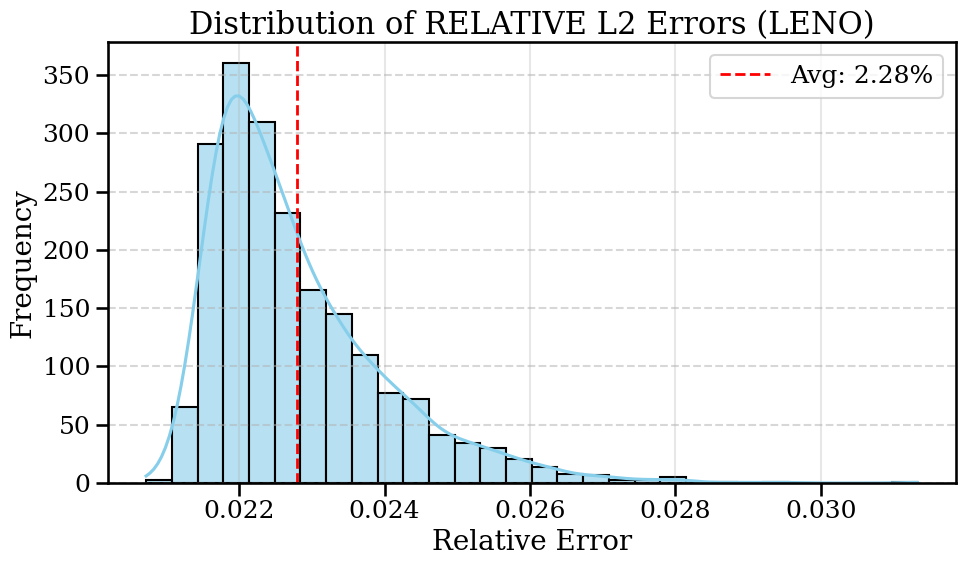
\includegraphics[width=\linewidth]{img/Allen-Cahn/Histograms/hist_test_set_leno_v2.png}
                \subcaption*{LENO}
            \end{minipage}
            \hfill
            \begin{minipage}[c]{0.46\textwidth}
                \centering
                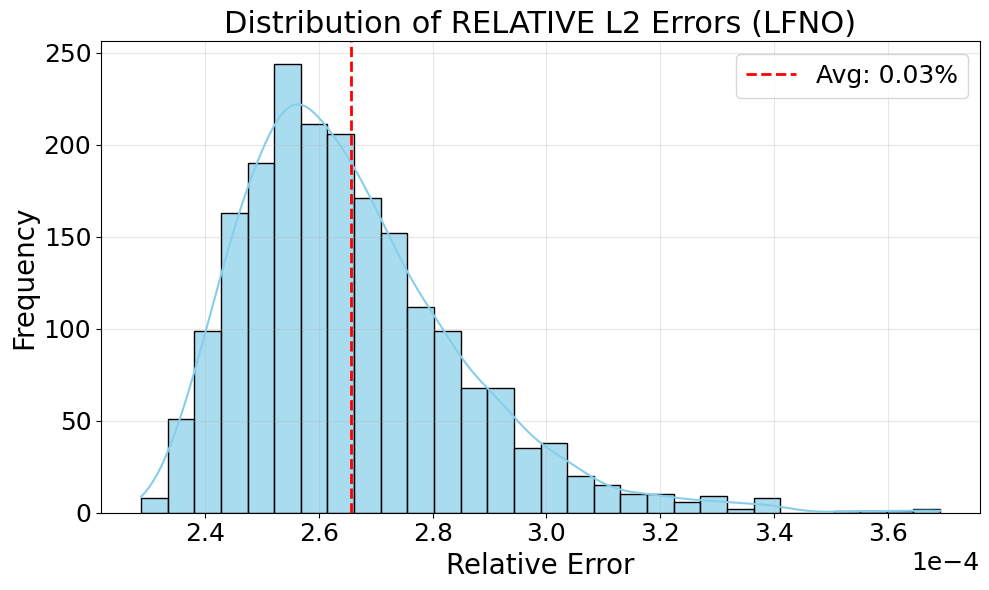
\includegraphics[width=\linewidth]{img/Allen-Cahn/Histograms/hist_test_set_LFNO_v2.png}
                \subcaption*{LFNO}
            \end{minipage}
            
        \end{minipage}
    } % Fine makebox
    
\caption{Matrix of Relative $L_2$ Error distributions on the test set.
    \textbf{Columns} distinguish between Nodal architectures (DeepONet family)%\protect\footnotemark 
     and Spectral architectures (FNO family). 
    \textbf{Rows} represent the hierarchy of inductive bias: Level 1 (Totally Blind), Level 2 (Physics-Informed), and Level 3 (Topology-Informed). 
    The red dashed line indicates the mean error. Note how the LFNO model (bottom right) achieves the lowest error variance and mean.}
    \label{fig:error_matrix}
\end{figure}



\begin{comment}
\begin{figure}[htbp]
    \centering
    
    % --- HEADERS (Struttura identica alle righe sotto) ---
    % 1. Spacer per l'etichetta verticale (0.05)
    \begin{minipage}{0.05\textwidth} 
        \hfill 
    \end{minipage}
    \hfill % <--- QUESTO MANCAVA! Allinea con lo spazio delle righe sotto
    % 2. DeepONet Title (0.46)
    \begin{minipage}{0.46\textwidth} 
        \centering \textbf{DeepONet Family}
    \end{minipage}
    \hfill % Spazio tra le due colonne principali
    % 3. FNO Title (0.46)
    \begin{minipage}{0.46\textwidth} 
        \centering \textbf{FNO Family}
    \end{minipage}
    \par\medskip

    % --- ROW 1: LEVEL 1 (BLIND) ---
    \begin{minipage}[c]{0.05\textwidth}
        \centering 
        \rotatebox{90}{\parbox{2.5cm}{\centering \textbf{Level 1} \\ (Blind)}}
    \end{minipage}
    \hfill
    \begin{minipage}[c]{0.46\textwidth}
        \centering
        
\includegraphics[width=\linewidth]{img/Allen-Cahn/Histograms/hist_test_set_deeponet_blind.png}
    \end{minipage}
    \hfill
    \begin{minipage}[c]{0.46\textwidth}
        \centering
        
\includegraphics[width=\linewidth]{img/Allen-Cahn/Histograms/hist_test_set_FNO_blind.png}
    \end{minipage}
    \par\bigskip 

    % --- ROW 2: LEVEL 2 (PHYSICS-INFORMED) ---
    \begin{minipage}[c]{0.05\textwidth}
        \centering 
        \rotatebox{90}{\parbox{2.5cm}{\centering \textbf{Level 2} \\ (Physics)}}
    \end{minipage}
    \hfill
    \begin{minipage}[c]{0.46\textwidth}
        \centering
        
\includegraphics[width=\linewidth]{img/Allen-Cahn/Histograms/hist_test_set_deeponet.png}
    \end{minipage}
    \hfill
    \begin{minipage}[c]{0.46\textwidth}
        \centering
        
\includegraphics[width=\linewidth]{img/Allen-Cahn/Histograms/hist_test_set_FNO.png}
    \end{minipage}
    \par\bigskip

    % --- ROW 3: LEVEL 3 (TOPOLOGY-INFORMED) ---
    \begin{minipage}[c]{0.05\textwidth}
        \centering 
        \rotatebox{90}{\parbox{2.5cm}{\centering \textbf{Level 3} \\ (Topology)}}
    \end{minipage}
    \hfill
    \begin{minipage}[c]{0.46\textwidth}
        \centering
        
\includegraphics[width=\linewidth]{img/Allen-Cahn/Histograms/hist_test_set_leno.png}
        \subcaption*{LENO}
    \end{minipage}
    \hfill
    \begin{minipage}[c]{0.46\textwidth}
        \centering
        
\includegraphics[width=\linewidth]{img/Allen-Cahn/Histograms/hist_test_set_LFNO.png}
        \subcaption*{LFNO}
    \end{minipage}
    
\caption{Matrix of Relative $L_2$ Error distributions on the test set.
    \textbf{Columns} distinguish between Nodal architectures (DeepONet family)%\protect\footnotemark 
     and Spectral architectures (FNO family). 
    \textbf{Rows} represent the hierarchy of inductive bias: Level 1 (Totally Blind), Level 2 (Physics-Informed), and Level 3 (Topology-Informed). 
    The red dashed line indicates the mean error. Note how the LFNO model (bottom right) achieves the lowest error variance and mean.}
    \label{fig:error_matrix}
\end{figure}
\end{comment}
%\footnotetext{\cite{wang2025laplacian} states that "our approach can be viewed as a variant of DeepONet, in which the trunk network is replaced by Laplacian eigenfunctions, while the branch network remains a linear functional approximated by a neural network."}
%%%%%%%%%%%%%%%%%%%%%%%%%%%%%%

The summary of the quantitative results is reported in Table \ref{tab:error_comparison}.


\begin{table}[htbp]
    \centering
    \begin{threeparttable} % <--- AGGIUNGI QUESTO WRAPPER
        \caption{Comparison of Mean Relative $L_2$ Errors on test set across all architectures. 
        The transition from Level 1 to Level 3 yields a massive error reduction (orders of magnitude). 
        Spectral methods (FNO family) generally outperform Nodal methods (DeepONet family).}
        \label{tab:error_comparison}

        \renewcommand{\arraystretch}{1.3}
        \setlength{\tabcolsep}{12pt}
        
        \begin{tabular}{lccc}
            \toprule
            \textbf{Inductive bias} & \textbf{Level} & \textbf{DeepONet family}\tnote{a} & \textbf{FNO family} \\ % Usa \tnote{a}
            \midrule
            
            \textbf{Totally blind} & 1 & $48 \pm 1$ \% & $27 \pm 1$\% \\
            \arrayrulecolor{black!30}\midrule 
            
            \textbf{Physics-informed} & 2 & $4.3 \pm 0.2$ \% & $0.070 \pm 0.002$ \% \\
            \arrayrulecolor{black!30}\midrule
    
            \textbf{Topology-informed} & 3 & $2.2 \pm 0.1$ \% \footnotesize{(LENO)} & $\mathbf{0.027 \pm 0.002}$ \textbf{\%} \footnotesize{(LFNO)} \\
            
            \arrayrulecolor{black}\bottomrule
        \end{tabular}
        
        % QUI DEFINISCI LA NOTA
        \begin{tablenotes}
            \small
            \item[a] LENO is effectively part of the DeepONet Family, since \cite{wang2025laplacian} states "our approach can be viewed as a variant of DeepONet, in which the trunk network is replaced by Laplacian eigenfunctions, while the branch network remains a linear functional approximated by a neural network."
        \end{tablenotes}
    \end{threeparttable}
\end{table}


%%%%%%%%%%%%%%%%%%%%%%%%%%
\begin{figure}[p] 
    \centering
    \setlength{\fboxsep}{0pt}
    
    % ==========================================
    % FAMILY 1: DeepONet
    % ==========================================
    
    % !!! FIX QUI: Titolo allineato alla colonna destra !!!
    % Usiamo una minipage vuota a sx per "spingere" il titolo al posto giusto
    \begin{minipage}{0.15\textwidth}
        \hfill % Vuoto
    \end{minipage}%
    \hspace{0.02\textwidth}%
    \begin{minipage}{0.75\textwidth}
        \centering
        \textbf{\large DeepONet family}
    \end{minipage}
    \par\vspace{0.2cm}
    
    % --- L1 ---
    \begin{minipage}{0.15\textwidth}
        \flushright \small \textbf{Level 1} \\ (Blind)
    \end{minipage}%
    \hspace{0.02\textwidth}%
    \begin{minipage}{0.75\textwidth}
        \centering
        
\includegraphics[height=0.135\textheight, keepaspectratio]{img/Allen-Cahn/Heatmaps/heatmap_DeepONet_Blind.png}
    \end{minipage}
    \par\vspace{0.1cm}
    
    % --- L2 ---
    \begin{minipage}{0.15\textwidth}
        \flushright \small \textbf{Level 2} \\ (Physics)
    \end{minipage}%
    \hspace{0.02\textwidth}%
    \begin{minipage}{0.75\textwidth}
        \centering
        
\includegraphics[height=0.135\textheight, keepaspectratio]{img/Allen-Cahn/Heatmaps/heatmap_DeepONet.png}
    \end{minipage}
    \par\vspace{0.1cm}

    % --- L3 ---
    \begin{minipage}{0.15\textwidth}
        \flushright \small \textbf{Level 3} \\ (Topology)
    \end{minipage}%
    \hspace{0.02\textwidth}%
    \begin{minipage}{0.75\textwidth}
        \centering
        
\includegraphics[height=0.135\textheight, keepaspectratio]{img/Allen-Cahn/Heatmaps/heatmap_leno.png}
        \\ \small \textit{LENO}
    \end{minipage}
    
    \par\vspace{0.4cm} % Separatore verticale tra le famiglie

    % ==========================================
    % FAMILY 2: FNO
    % ==========================================

    % !!! FIX QUI: Titolo allineato alla colonna destra !!!
    \begin{minipage}{0.15\textwidth}
        \hfill % Vuoto
    \end{minipage}%
    \hspace{0.02\textwidth}%
    \begin{minipage}{0.75\textwidth}
        \centering
        \textbf{\large FNO family}
    \end{minipage}
    \par\vspace{0.2cm}

    % --- L1 ---
    \begin{minipage}{0.15\textwidth}
        \flushright \small \textbf{Level 1} \\ (Blind)
    \end{minipage}%
    \hspace{0.02\textwidth}%
    \begin{minipage}{0.75\textwidth}
        \centering
        
\includegraphics[height=0.135\textheight, keepaspectratio]{img/Allen-Cahn/Heatmaps/heatmap_FNO_blind.png}
    \end{minipage}
    \par\vspace{0.1cm}

    % --- L2 ---
    \begin{minipage}{0.15\textwidth}
        \flushright \small \textbf{Level 2} \\ (Physics)
    \end{minipage}%
    \hspace{0.02\textwidth}%
    \begin{minipage}{0.75\textwidth}
        \centering
        
\includegraphics[height=0.135\textheight, keepaspectratio]{img/Allen-Cahn/Heatmaps/heatmap_FNO.png}
    \end{minipage}
    \par\vspace{0.1cm}

    % --- L3 ---
    \begin{minipage}{0.15\textwidth}
        \flushright \small \textbf{Level 3} \\ (Topology)
    \end{minipage}%
    \hspace{0.02\textwidth}%
    \begin{minipage}{0.75\textwidth}
        \centering
        
\includegraphics[height=0.135\textheight, keepaspectratio]{img/Allen-Cahn/Heatmaps/heatmap_LFNO.png}
        \\ \small \textit{LFNO}
    \end{minipage}

    \par\vspace{0.2cm}
    
    \caption{Sequential comparison of Error Heatmaps. Top block: DeepONet architectures; Bottom block: FNO architectures.}
    \label{fig:heatmap_vertical_stack}
\end{figure}



%%%%%%%%%%%%%%%%%%%%%%%%%%
\begin{table}[htbp]
    \centering
    \renewcommand{\arraystretch}{1.3} 
    \setlength{\tabcolsep}{14pt} 
    
    \begin{tabular}{lcc}
        \toprule
        \multirow{2.5}{*}{\textbf{Inductive bias}} & \multicolumn{2}{c}{\textbf{Learned} $\boldsymbol{\nu}$} \\
        \cmidrule(lr){2-3} % Linea che copre solo le colonne dei dati
        & \textbf{DeepONet family} & \textbf{FNO family} \\
        \textit{(Level)}\\
        \midrule
        
        \textbf{Physics-informed} & \multirow{2}{*}{$3.334$} & \multirow{2}{*}{$4.002$} \\
        (Level 2) & & \\
        
        \arrayrulecolor{black!30}\midrule 
        
        \textbf{Topology-informed} & \multirow{2}{*}{$3.526$} & \multirow{2}{*}{$\mathbf{3.998}$} \\
        (Level 3) & \small{\textit{(LENO)}} & \small{\textit{(LFNO)}} \\
        
        \arrayrulecolor{black}\bottomrule
    \end{tabular}
    
    \caption{System Identification Results. Comparison of the learned diffusion coefficient $\nu$ (Ground Truth $\nu = 4.000$). 
    Values are rounded to 4 significant figures. 
    Spectral architectures (FNO family) successfully identify the correct physical parameter with high precision, 
    whereas Nodal architectures (DeepONet family) tend to underestimate it.}
    \label{tab:learned_coeffs}
\end{table}
%%%%%%%%%%%%%%%%%%%%%%%%%%

%%%%%%%%%%%%%%%%%%%%%%%%%%%%%%%%%%%%%%%%%%%%%%%%
\newpage

\subsection{Discussion}

The results presented in this section clearly demonstrate the significant impact of incorporating inductive biases into neural operator architectures
 for learning dynamics on complex networks.

 In fact both blind architectures (Level 1) exhibit poor generalization capabilities, with mean relative $L_2$ errors of $48\%$ (DeepONet) and $27\%$ (FNO).

On the other hand, adding physical information (Level 2) drastically reduced the error by orders of magnitude.
Evidently, embedding the underlying physics of the system into the learning process is crucial for accurate predictions.

It is worth noting that in Level 2, even if we didn't insert topological information in the neural network,
we still exploited the Laplacian operator in the integration scheme. So, if we hadn't had access to the topological features we would have needed another integration method, which probably would have lowered the performances.

This performance difference can be attributed to how the two architectures manage physical and spectral representations. The FNO family inherently leverages a dual-domain representation: it receives physical nodal features as input, processes them within an internal spectral representation (the hidden layers utilizing the FFT/ GFT), and crucially, projects the output back via the inverse FFT/ GFT to compute the loss directly in the physical domain. In contrast, the evaluated DeepONet architectures are restricted to a single domain during optimization: standard DeepONets (Levels $1$ and $2$) operate exclusively on artificial spatial coordinates, while the baseline LE-NO (Level $3$) computes both its predictions and its loss entirely within the spectral domain, losing direct supervision on the physical nodal states.


\section{Example 2: the case of FitzHugh-Nagumo}
\label{sec:Example 2}
\subsection{Motivation}
After this first implementation we asked ourselves two questions: Can we generalize this architecture to more than one variable? 
Is it possible to extract information about $\mathbf{F}(\mathbf{u})$ from the trained NN?
\newline
%Scriverò qualcosa a proposito nell'introduzione
In particular this last problem is part of the \textbf{PDE discovery}, mentioned in Chapter \ref{Chp:2}.

In this section we considered again our neural system, described by Eq. \eqref{eq:coupled_FHN}.

However we changed the setup by \textbf{removing the input current} and randomly uniform initial state $\left( V_i\left( 0 \right), w_i\left( 0 \right) \right) \in \left[-1, 1  \right]^2$ for each node $i$.

Then, given a graph $\mathcal{G} = (\mathcal{V}, \mathcal{E})$:
\begin{equation}
\label{eq:coupled_FHN2}
\begin{aligned}
\frac{dV_i}{dt} &= b V_i (V_i - \beta)(\delta - V_i) - c w_i - D_V \sum_{j=1}^{|\mathcal{V}|} L_{ij} V_j \\
\frac{dw_i}{dt} &= \epsilon (V_i - \gamma w_i) \\
V_i\left( 0 \right) &= V_i^0 \\
w_i\left( 0 \right) &= w_i^0
\end{aligned}
\end{equation}

Where the parameters are $b = 5$, $c = 1$, $\beta = 0.1$, $\delta = 1$, $\epsilon = 0.1$, $\gamma = 0.25$, as in \cite{centofanti2024comconf} and $i \in \{1, \dots, |\mathcal{V}|\}$ represents the node of interest.


\subsection{Graph topology}
We generated a scale-free network using the \textbf{Barabási-Albert (BA)} model to mimic realistic topological features such as hubs and clusters.
\begin{itemize}
    \item \textbf{Nodes:} $N = 1000$.
    \item \textbf{Attachment:} $m = 2$.
\end{itemize}

\subsection{Dynamics: FitzHugh-Nagumo on graphs}
The reaction kinetics for the two-variable FHN model, consisting of an activator $V$ and an inhibitor $w$, are defined by (as in Eq. \eqref{eq:coupled_FHN2}):
\begin{equation}
\begin{aligned}
    \mathbf{F}_V(V, w) &= b V (V - \beta)(\delta - V) - c w \\
    \mathbf{F}_w(V, w) &= \epsilon (V - \gamma w)
\end{aligned}
\end{equation}

Diffusion was applied solely to the activator variable ($D_V = 0.01$), while the inhibitor remained strictly localized ($D_w = 0$).

The system evolved from random initial conditions, with both $V$ and $w$ independently sampled from a uniform distribution $\mathcal{U}(-1, 1)$ across all nodes. We generated a large-scale dataset of $15000$ trajectories ($10000$ for training, $2000$ for validation, $1000$ for hyperparameter tuning, and $2000$ for testing). The system was numerically integrated over $150$ time steps with a temporal resolution of $\Delta t = 0.05$ (yielding a total simulation time of $T=7.5$s) to create the input-target pairs.
In Figure \ref{fig:fhn_dynamics} we can observe the evolution of the system. Note that for both variables $V$ and $w$ the system creates spatial patters of zones at different equilibria.

\begin{figure}[htbp]
    \centering
    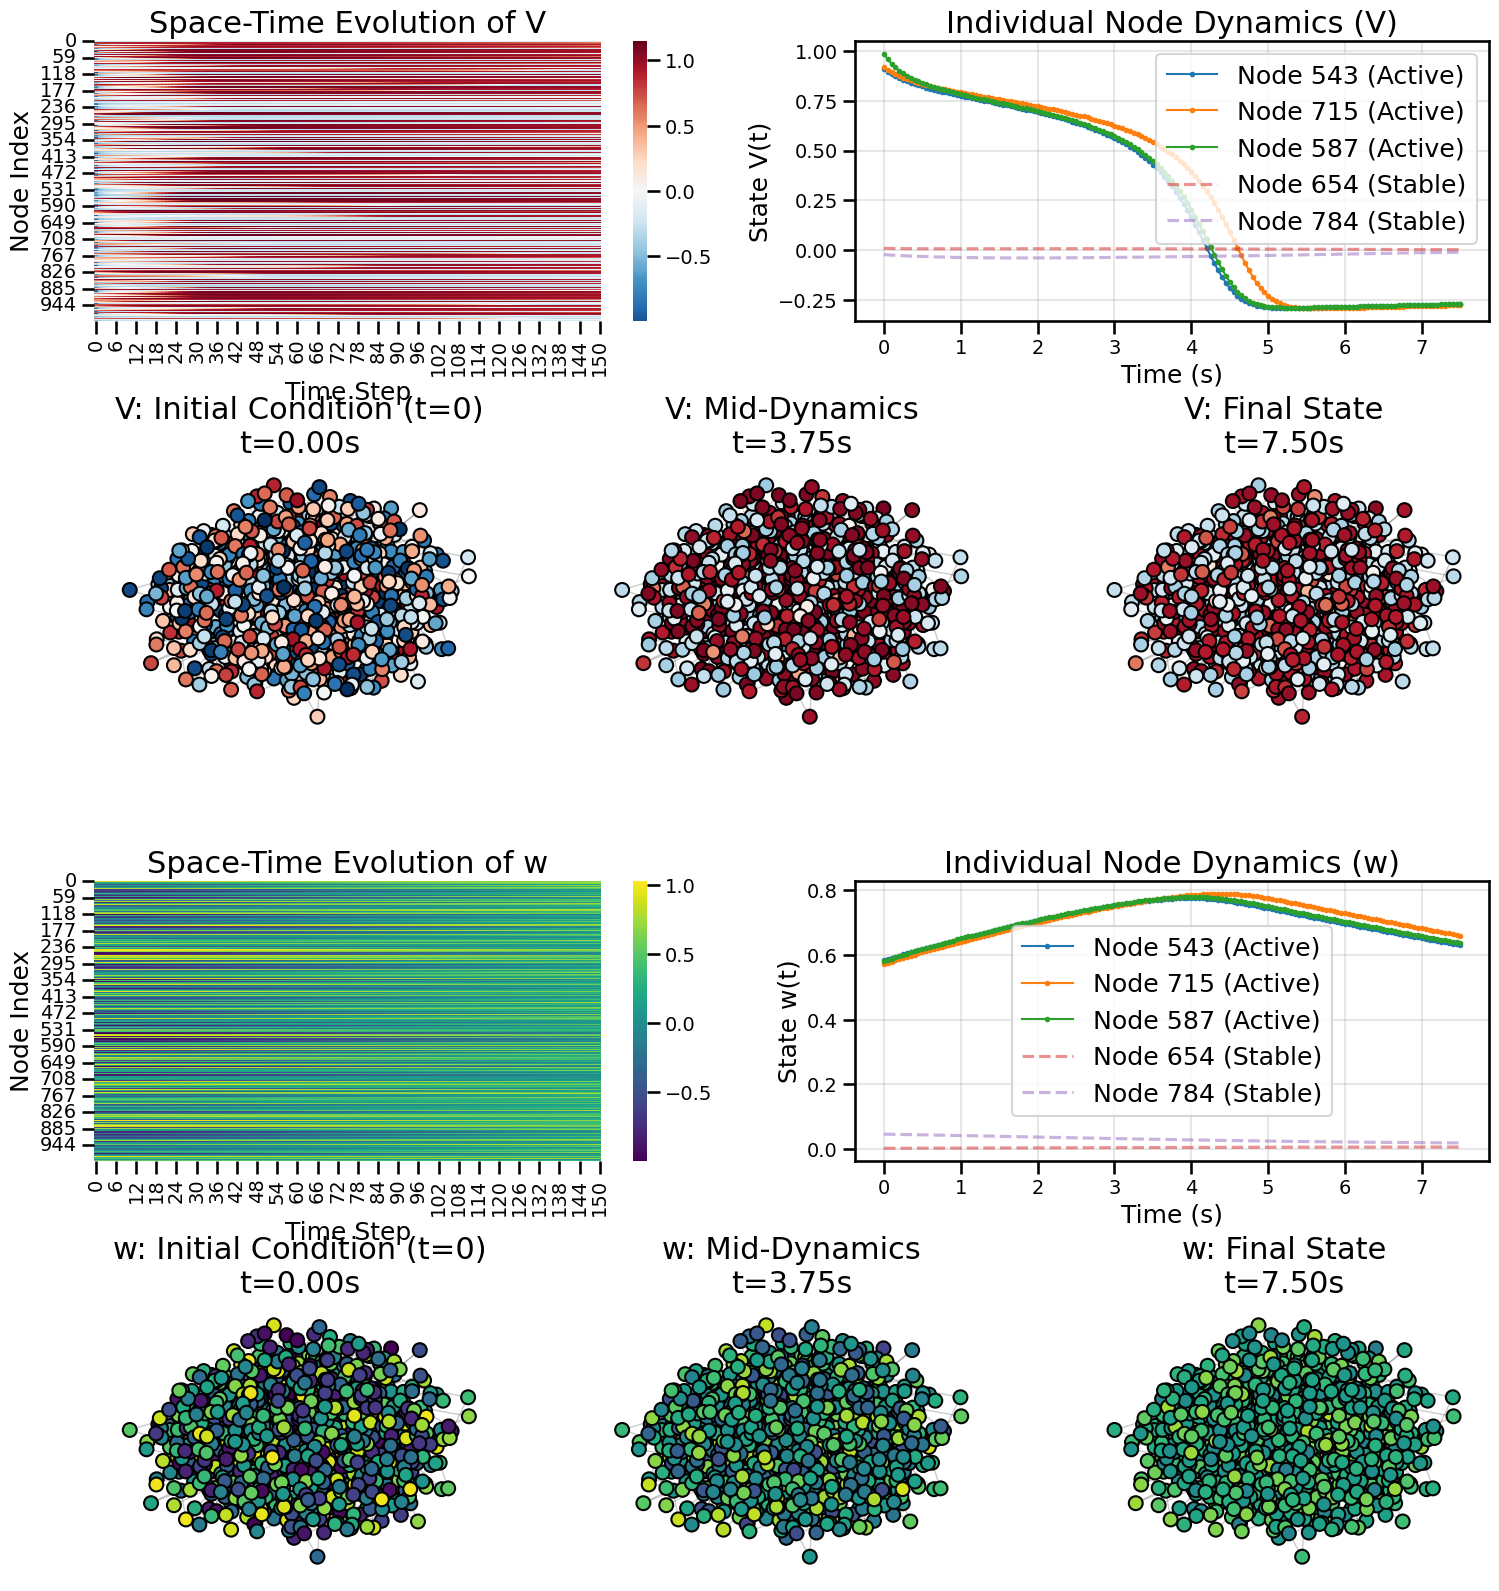
\includegraphics[width=1.0\textwidth]{img/LFNO_FH/dynamics.png}
    \caption{Simulation of the coupled FitzHugh-Nagumo dynamics on a Barabási-Albert graph ($N=1000$, $m=2$). The figure illustrates the space-time evolution, individual node trajectories, and network-wide states for both the activator ($V$, top rows) and inhibitor ($w$, bottom rows) variables, highlighting the distinct non-linear coupled behavior over the $7.5$s simulation window.}
    \label{fig:fhn_dynamics}
\end{figure}

\newpage
\subsection{Training details}
All models were implemented in PyTorch and trained on a dedicated GPU to accelerate tensor operations and spectral transformations. To ensure strict reproducibility, fixed global random seeds ($42$) were explicitly enforced across all data generation and training experiments.

The network parameters were optimized using the Adam algorithm with a weight decay of $10^{-4}$ and a gradient clipping threshold of $1.0$ to ensure numerical stability.
To efficiently manage memory and computational load during the full-horizon rollout, we employed a dual mini-batch strategy: a batch size of $32$ was used for unrolling the trajectory, while a larger batch of $1024$ points was sampled to evaluate the physics-informed residual loss. Both the trajectory tracking and the PDE residual objectives were computed using a relative $L_2$ norm metric to equally balance the contribution of the two FHN variables \footnote{This is consistent with the best found prefactor for the physics loss term $\lambda_{phys}=1$}.

To select the optimal configuration, we performed an automated hyperparameter search using the \textit{Optuna} framework, utilizing a \textit{Median Pruner} to early-stop unpromising trials. Based on this search, the selected hyperparameter configuration for the coupled FitzHugh-Nagumo system was set as follows:
\begin{itemize}
    \item Initial learning rate: $\eta = 7 \cdot 10^{-4}$;
    \item Physics penalty weight: $\lambda_{\text{phys}} = 1.0$;
    \item Initial guesses for the simultaneous system identification of the diffusion coefficients ($D = \varepsilon^2$): we initialized $\varepsilon_{V,\text{init}} = 0.5$ for the activator and $\varepsilon_{w,\text{init}} = 0.3$ for the inhibitor;
    \item Architecture-specific hyperparameters: the spectral layers were configured to retain $330$ Fourier modes with a hidden channel width of $64$.
\end{itemize}

Once the best hyperparameters were identified, the final model was trained for $100$ epochs. The learning rate was scheduled to decay by a factor of $\gamma = 0.5$ every $30$ epochs to refine the convergence. 
To prevent overfitting, we continuously monitored the relative error on the validation set, ensuring that the model weights and the learned physical parameters ($\varepsilon_V, \varepsilon_w$) were saved precisely at the epoch that yielded the lowest validation loss.



\subsection{Results}

The training dynamics of the two-variable LFNO model demonstrate stable and robust convergence. As depicted in the learning curves (Figure \ref{fig:lfno_loss}), both the training and validation losses decrease monotonically on a logarithmic scale. The validation-based checkpointing successfully prevented overfitting, identifying epoch $96$ as the optimal state of the network with the lowest validation error. Since this value is close to the total number of epochs $100$, it is probable that the model could find an even better optimum with a higher number of iterations.

In addition to accurate trajectory prediction, the proposed Operator Learning framework naturally supports \textit{System Identification}. Because the physical diffusion operator is explicitly embedded within the spectral layers, the diffusion coefficients ($\varepsilon_V$ and $\varepsilon_w$) can be simply treated as learnable parameters rather than fixed constants. As illustrated in Figure \ref{fig:lfno_diffusion}, these parameters rapidly converge to their true physical values (accurate to four decimal places) within the very first epochs. The network correctly identifies that the activator $V$ diffuses with $D_V = 0.01$, while accurately recognizing that the inhibitor $w$ is strictly localized ($D_w = 0.00$).

\begin{figure}[htbp]
    \centering
    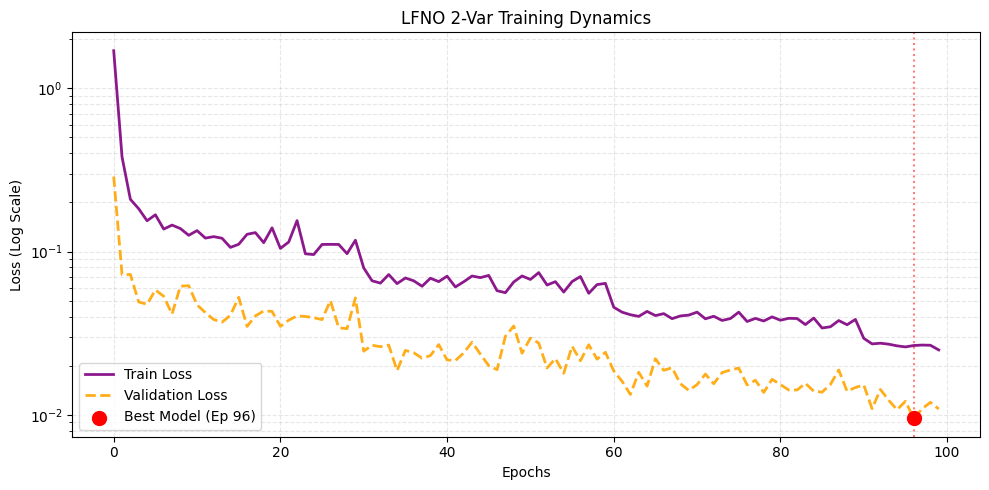
\includegraphics[width=0.85\textwidth]{img/LFNO_FH/loss.png}
    \caption{Training and validation loss curves (MSE). The optimal model weights were extracted at epoch 96 (red marker).}
    \label{fig:lfno_loss}
\end{figure}

\begin{figure}[htbp]
    \centering
    \begin{minipage}{0.48\textwidth}
        \centering
        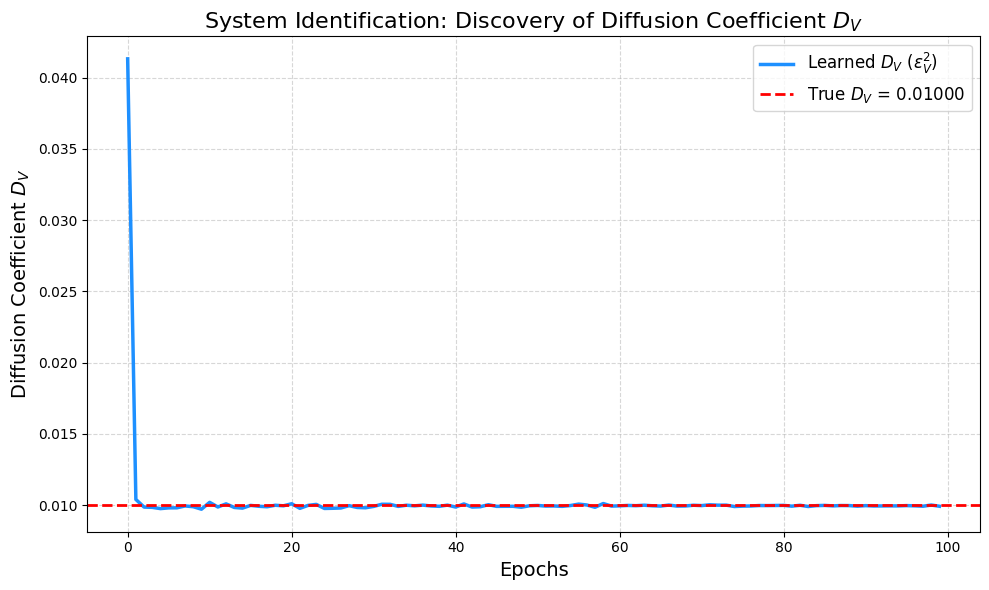
\includegraphics[width=\textwidth]{img/LFNO_FH/Diffusion_coefficient_V.png}
    \end{minipage}\hfill
    \begin{minipage}{0.48\textwidth}
        \centering
        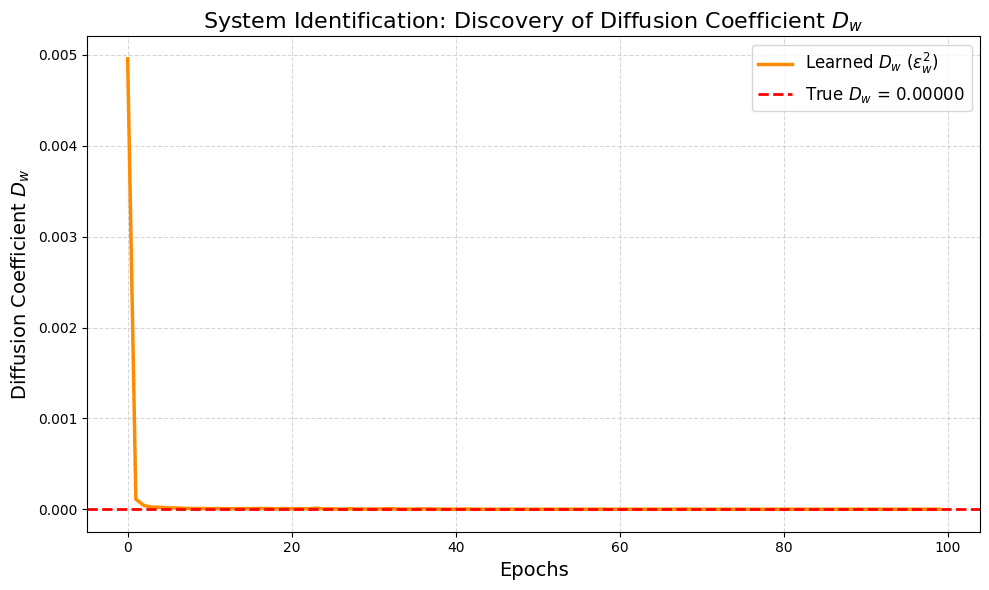
\includegraphics[width=\textwidth]{img/LFNO_FH/Diffusion_coefficient_w.png}
    \end{minipage}
    \caption{System identification of the diffusion coefficients. The network accurately discovers both $D_V = 0.01$ (left) and $D_w = 0.0$ (right) in less than 5 epochs.}
    \label{fig:lfno_diffusion}
\end{figure}

To quantitatively assess the generalization capabilities of the trained model, we evaluated it on a strictly held-out test set. The histogram of the relative $L_2$ errors (figure \ref{fig:lfno_hist}) exhibits a very low mean and variance. The model achieves an outstanding average relative $L_2$ error of just $(0.8 \pm 0.4)\%$, confirming that the LFNO has successfully learned the continuous operator mapping rather than merely memorizing the training trajectories.

\begin{figure}[htbp]
    \centering
    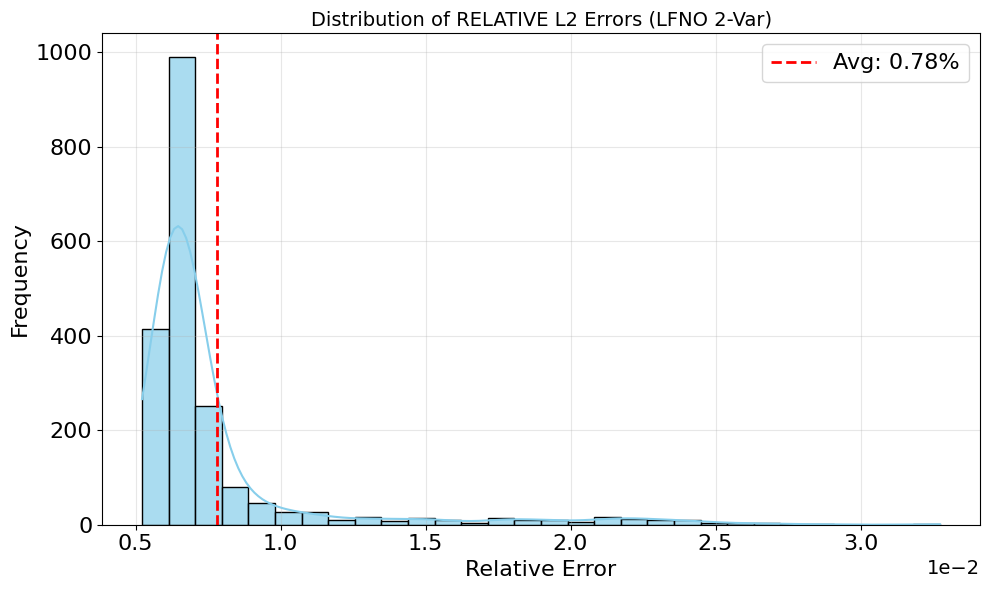
\includegraphics[width=0.75\textwidth]{img/LFNO_FH/Hist_test_set.png}
    \caption{Distribution of the Relative $L_2$ errors evaluated on the unseen test trajectories. The extremely low average error highlights the strong predictive power of the model.}
    \label{fig:lfno_hist}
\end{figure}

Finally, qualitative assessments further validate the numerical results. The space-time heatmaps (Figure \ref{fig:lfno_heatmaps}) show a near-perfect visual overlap between the ground truth and the LFNO predictions for both the activator and the inhibitor variables across the entire network. The absolute error maps remain orders of magnitude lower than the signal amplitude (Mean Absolute Error of $1.09 \times 10^{-3}$ for $V$ and $4.85 \times 10^{-4}$ for $w$). This high fidelity is also evident when zooming in on the continuous dynamics of individual nodes (Figure \ref{fig:lfno_nodes}), where the predicted trajectories (dashed lines) seamlessly track the non-linear physiological behavior of the exact simulated system without any phase shifts or amplitude degradation.

\begin{figure}[htbp]
    \centering
    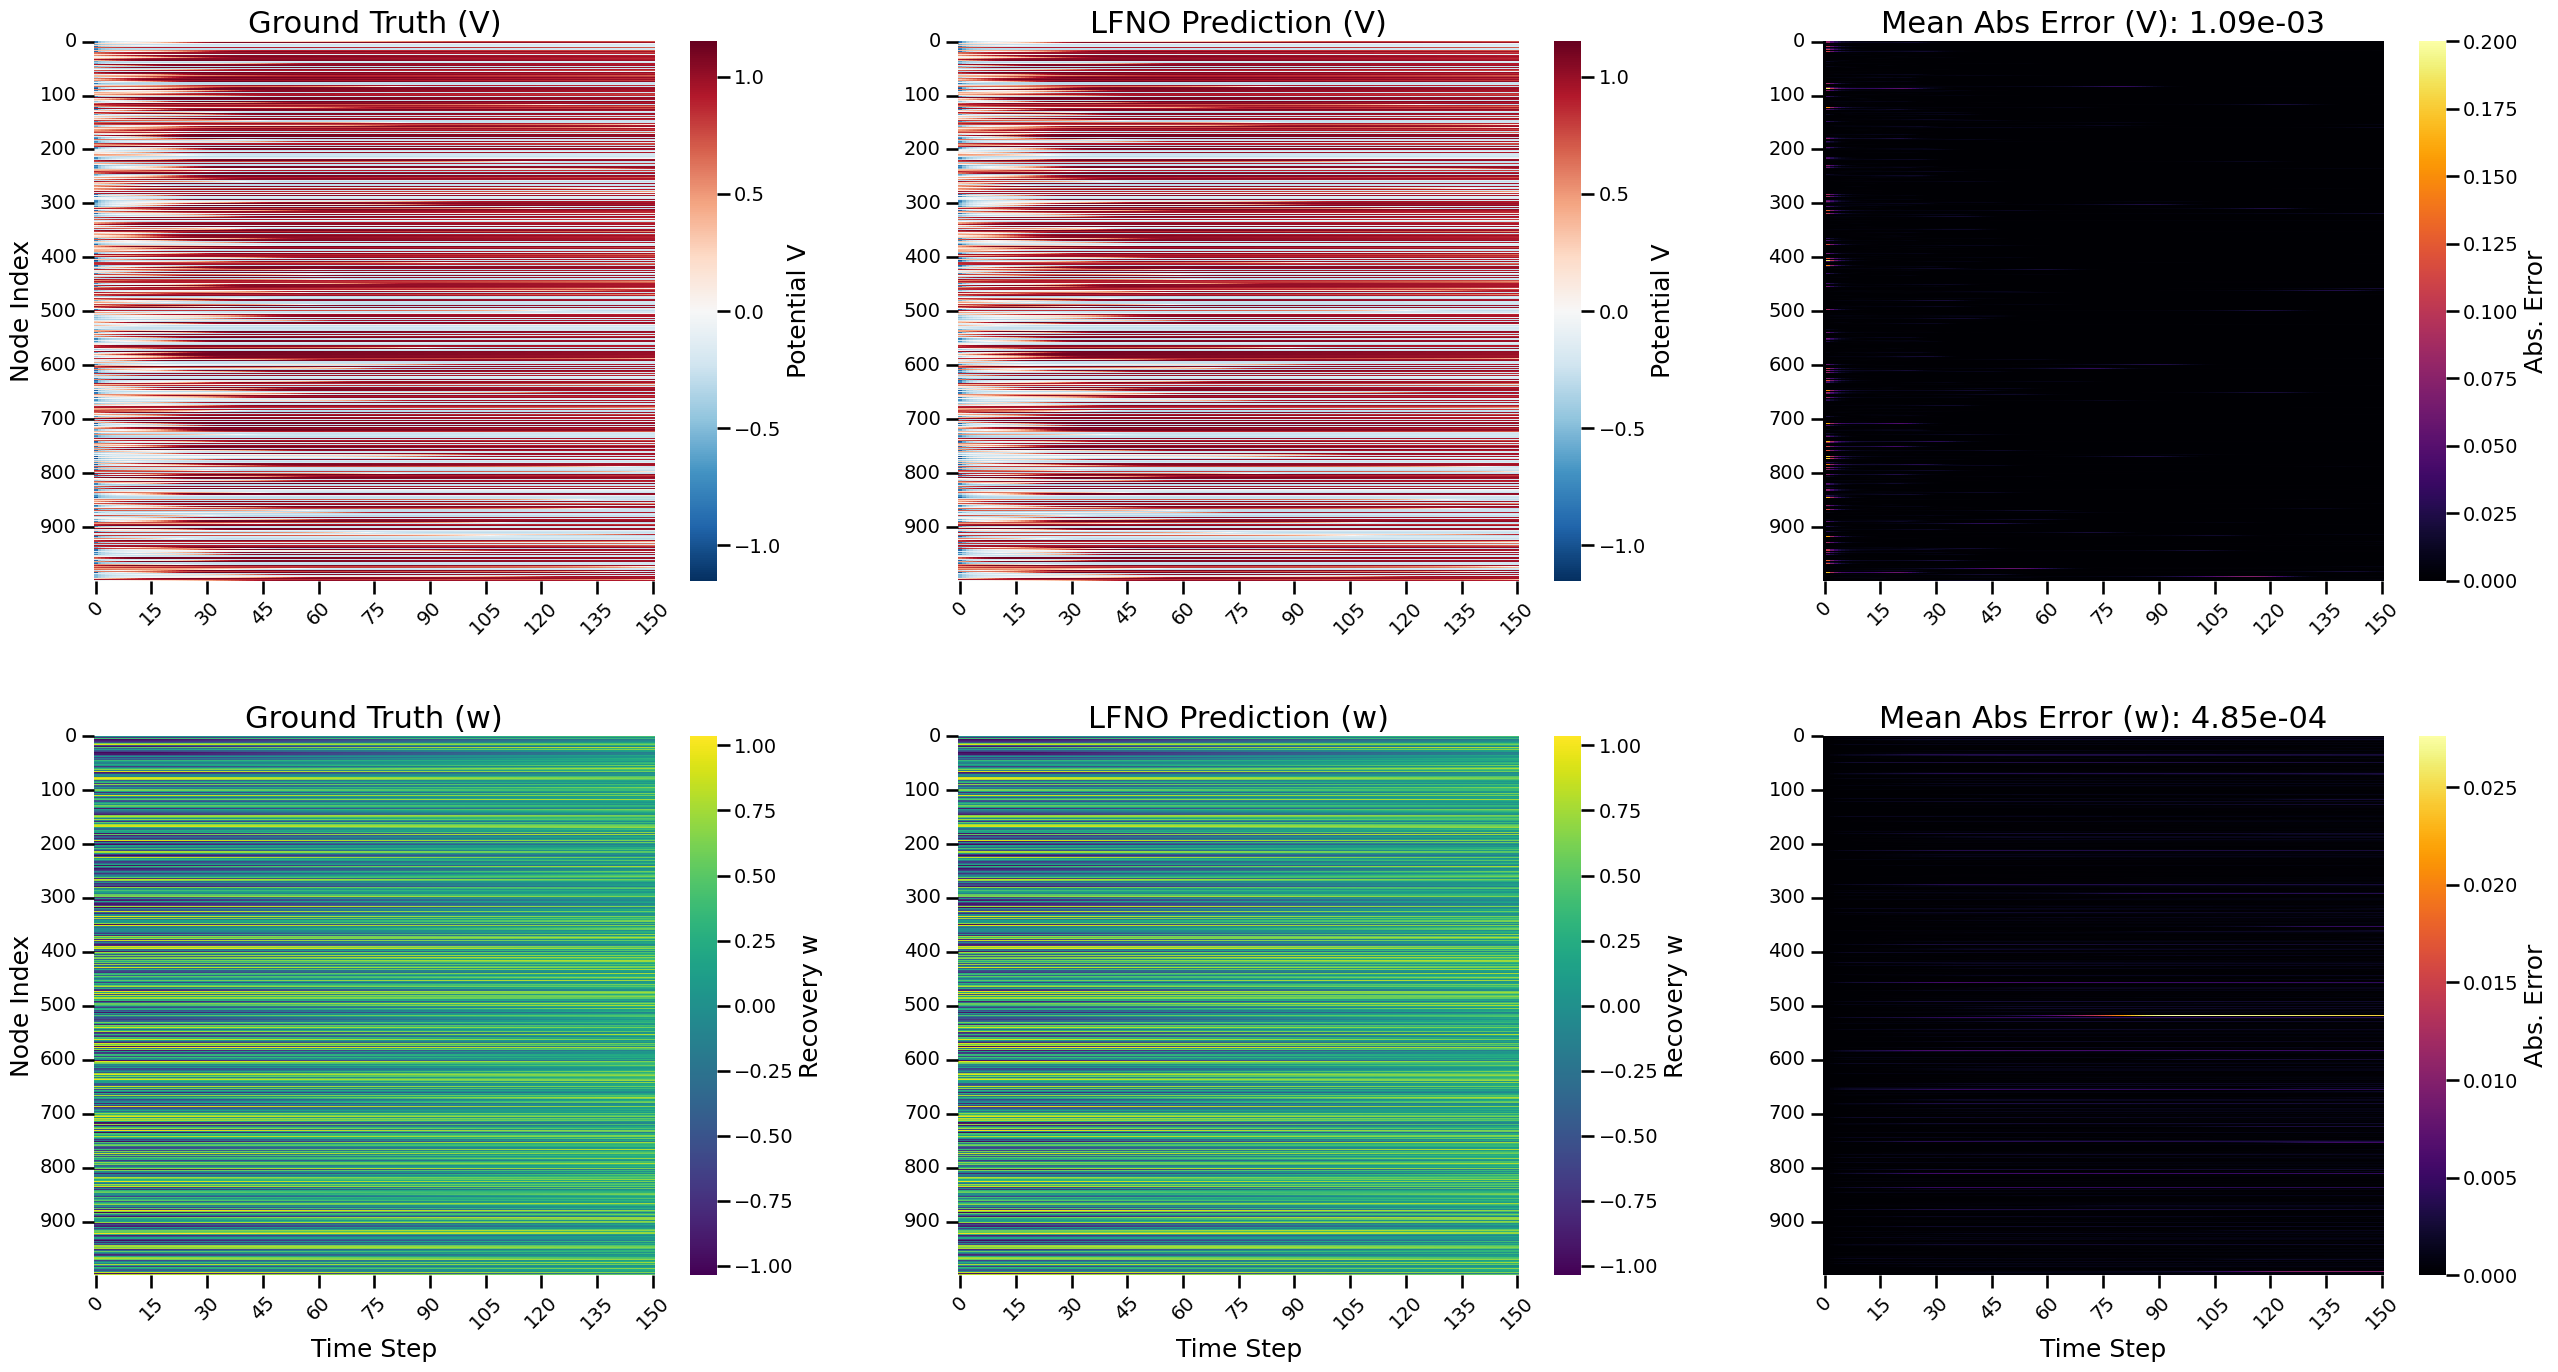
\includegraphics[width=\textwidth]{img/LFNO_FH/Results_test_set.png}
    \caption{Space-time evolution of a typical test trial. The LFNO reconstructions (center) are virtually indistinguishable from the ground truth (left). The absolute error (right) is negligible.}
    \label{fig:lfno_heatmaps}
\end{figure}

\begin{figure}[htbp]
    \centering
    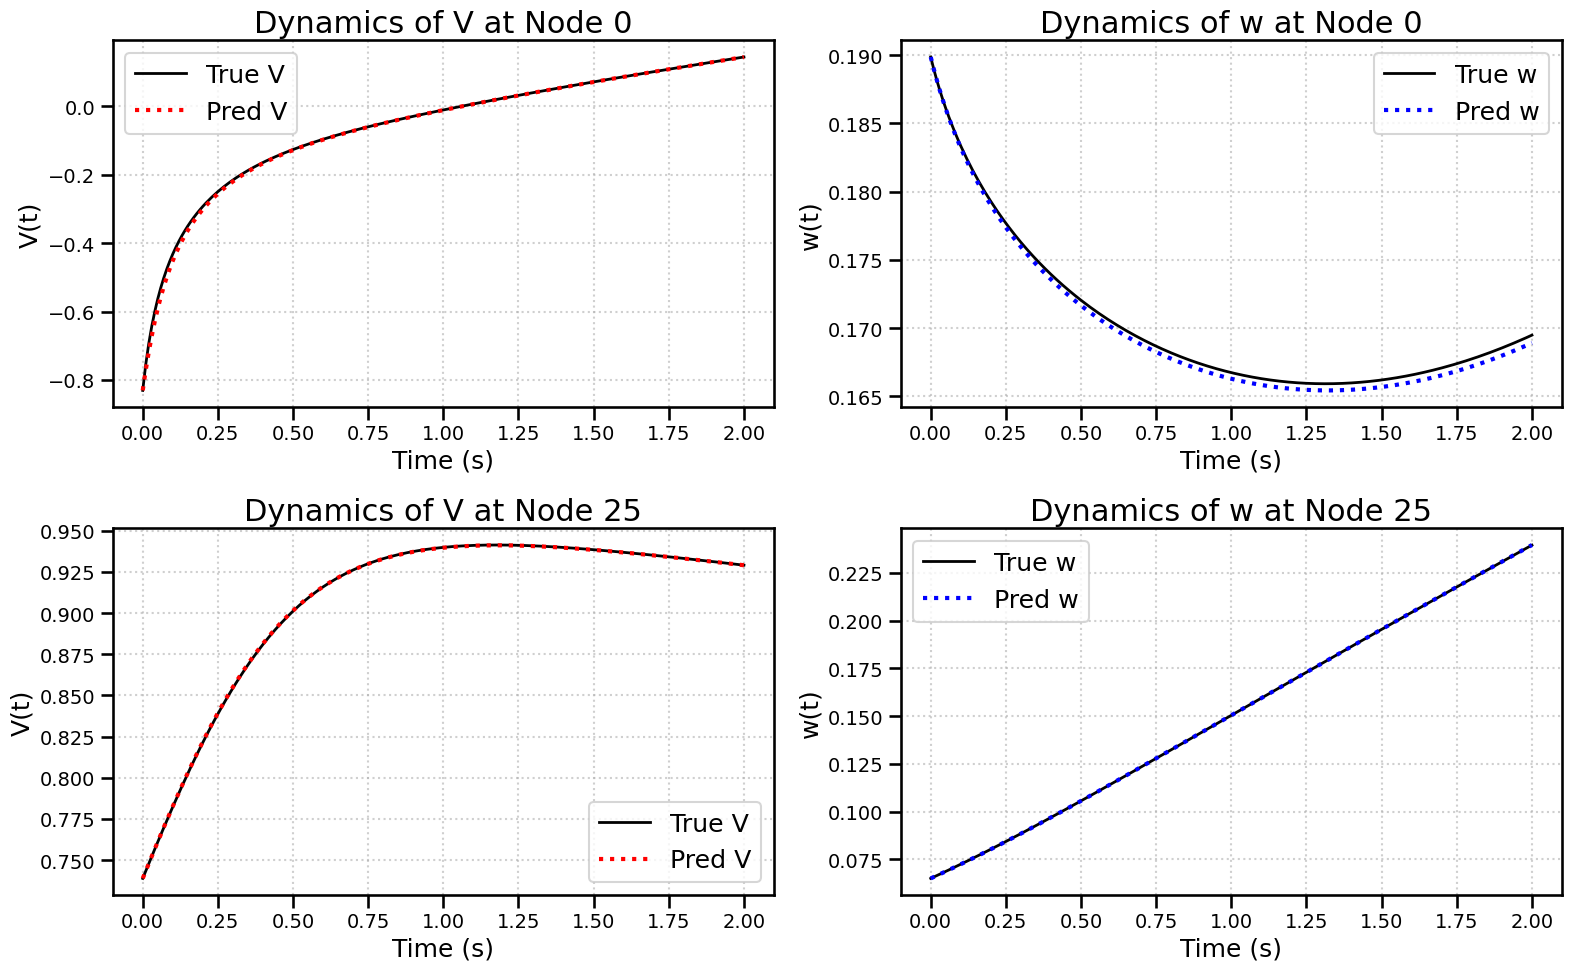
\includegraphics[width=0.9\textwidth]{img/LFNO_FH/Results_single_nodes_test_set_v2.png}
    \caption{Continuous temporal dynamics of individual selected nodes. The LFNO predictions perfectly capture the non-linear, coupled evolution of both $V$ and $w$.}
    \label{fig:lfno_nodes}
\end{figure}

\newpage
\subsection{The inverse problem}
\label{sec:Inverse Problem}

Beyond forward trajectory prediction and system identification of scalar parameters, the proposed architecture allows us to inspect the learned continuous operators. This direction, to our knowledge, has not been explored in the literature yet. 
\newline
Specifically, we can isolate the non-linear reaction terms learned by the network and evaluate them on a discrete 2D grid of $(V, w)$ phase space, comparing them directly against the exact analytical functions $F_V(V, w)$ and $F_w(V, w)$. 

As shown in Figure \ref{fig:lfno_reactions}, the network successfully reconstructs the reaction surfaces. On the naturally explored phase space, the model achieves a relative $L_2$ error of $3.89\%$ for the activator kinetics $F_V(V,w)$ and $1.08\%$ for the inhibitor kinetics $F_w(V,w)$. These low error margins demonstrate that the network is genuinely solving the inverse problem by discovering the underlying governing equations.

However, the metrics reported above are calculated on a grid spanning the specific domain of states predominantly visited during the simulated time horizon, which is not symmetrically distributed. If the learned reaction function $F_V(V,w)$ is evaluated uniformly over the entire $[-1, 1] \times [-1, 1]$ domain, its performance degrades significantly in the negative extreme. In fact if we look at Figure \ref{fig:lfno_reactions2} we can note that the error increases to $23.94\%$ for $F_V(V,w)$, while it remains at $3.45\%$ for $F_w(V,w)$.
\newline
 This limitation is physically grounded: as previously observed in the spatio-temporal dynamics, the $V=-1$ region represents a highly unstable region of the FitzHugh-Nagumo phase portrait. Consequently, the training trajectories rapidly transition away from these states, leaving the neural network with a severe lack of data support in that specific region \footnote{We suppose this doesn't happen around the $V=1$ region both because of the specific initialization and because the gradient is less steep. Morover, increasing the temporal resolution of the simulation may solve this problem. This theory will be subject of future investigations.}. Without sufficient observations, the model cannot accurately extrapolate the cubic curvature of $F_V$, highlighting a fundamental limitation of data-driven inverse modeling in strictly transient or unstable regimes.


\begin{figure}[htbp]
    \centering
    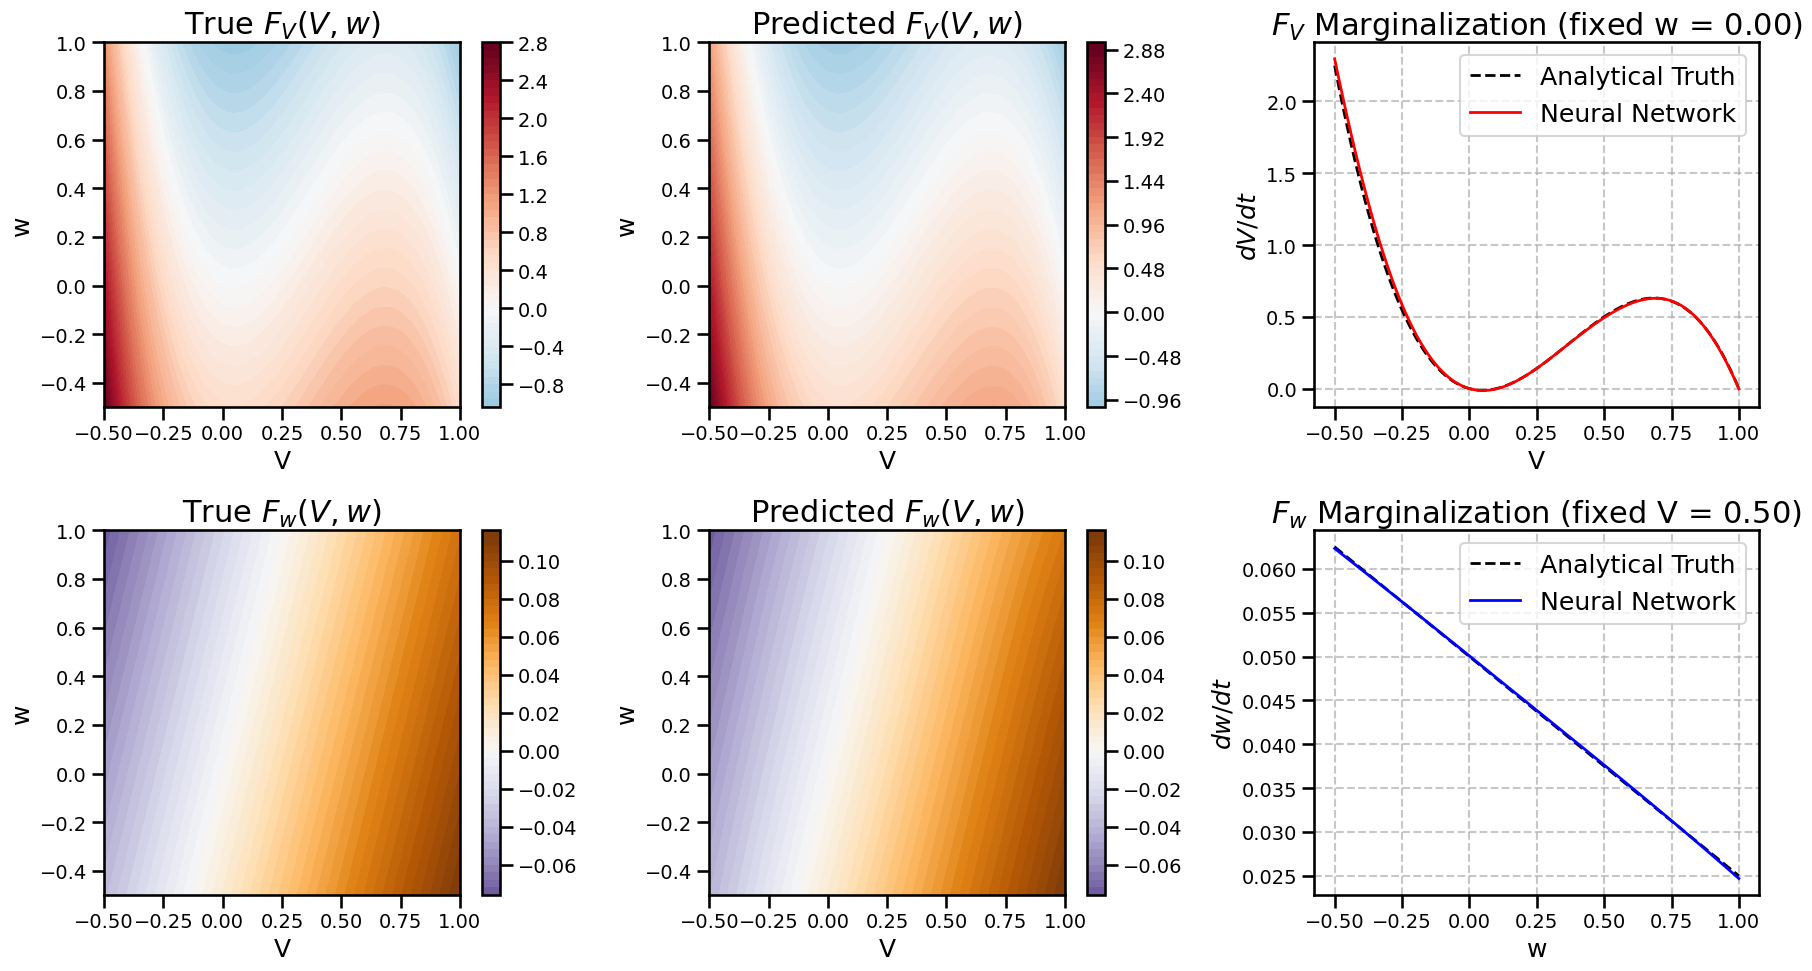
\includegraphics[width=\textwidth]{img/LFNO_FH/Reactions_fit.png}
    \caption{Analytical vs. Learned reaction functions evaluated on the 2D phase space grid $[-0.5,1]^2$}
    \label{fig:lfno_reactions}
\end{figure}

\begin{figure}[htbp]
    \centering
    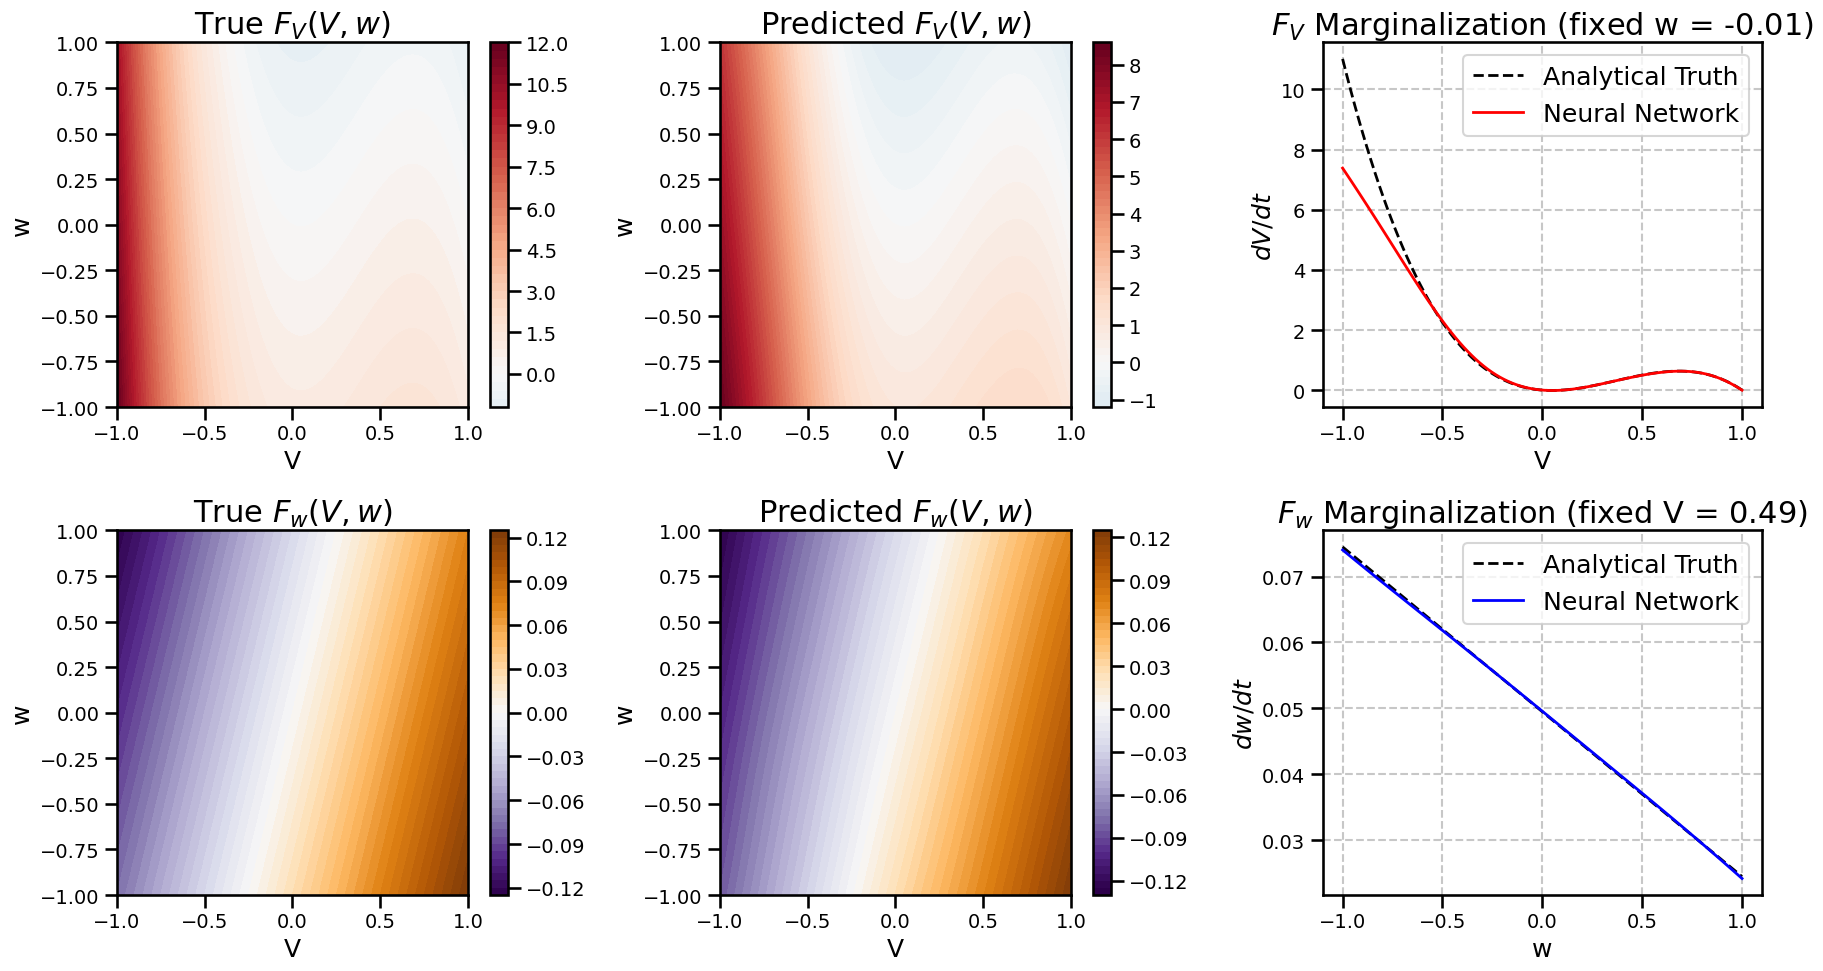
\includegraphics[width=\textwidth]{img/LFNO_FH/Reactions_fit_[-1,1].png}
    \caption{Analytical vs. Learned reaction functions evaluated on the 2D phase space grid $[-1,1]^2$. While the network accurately captures the governing equations in the highly sampled regions, the approximation degrades in the unstable, sparsely sampled domains (e.g., near $V=-1$).}
    \label{fig:lfno_reactions2}
\end{figure}
    
 %   \input{chapters/demo-filler}

    % conclusion ---------------
    %!TEX root = ../main.tex

\chapter*{\label{ch:conclusions}Conclusions}
\markboth{Conclusions}{}
\addcontentsline{toc}{chapter}{Conclusions} 
% NOTE: Introduction and Conclusions are special chapters: they are not
%       marked by a section number, so we need to add it manually to the
%       ToC, as done above.

Building upon the theoretical foundations of neuroscientific models (Chapter 1) and Scientific Machine Learning (Chapter 2), Chapter 3 demonstrated the expressive fitting power of Operator Learning on both synthetic and empirical data. Regarding the synthetic approach, an interesting avenue for future research would be to determine the maximum network size, $N$, up to which the performance of our setup remains stable. Conversely, concerning real-world applications, future efforts should focus on refining neural operator architectures to achieve the quantitative precision required for clinical translation. Specifically, minimizing this error profile will enable the development of model-free anomaly detection systems. Trained exclusively on baseline data from healthy subjects, these refined operators could identify subtle, statistically significant deviations in neural output, thereby serving as non-invasive diagnostic tools for neurological disorders. Furthermore, the generalizability of these models warrants testing across adjacent domains, including computational social science and bioinformatics.

Finally, Chapter 4 demonstrated that expressive power and interpretability can successfully coexist. In this context, an important benchmark omitted from this study is the Graph Neural Network (GNN), which naturally processes network structures via message-passing operations. It would be valuable to evaluate whether the LFNO outperforms the GNN when both are deployed within our framework. Furthermore, due to time constraints, the performance of the LFNO has yet to be benchmarked against empirical datasets. A key milestone for future research will be validating the LFNO framework on large-scale real-world data, such as modeling epidemic propagation across the complex network of Italian regional connections.

Crucially, the most promising and mathematically profound extension of this work lies in the reverse-engineering of underlying physical laws directly from observational data (Section \ref{sec:Inverse Problem}). By exploiting the trained LFNO, we reconstructed the reaction potentials of interacting species, mapping the data onto an empirical hypersurfaces within the system's phase space. Through the subsequent application of symbolic regression, we anticipate distilling these learned hypersurfaces into explicit, closed-form analytical expressions derived purely from data. In an epidemiological context, this translates to discovering the exact functional forms of transmission and recovery rates directly from noisy surveillance data, without relying on prior mechanistic assumptions. Beyond this inverse problem, future projects will explore inferring hidden network topologies when reaction terms are known, quantifying the model's robustness against topological uncertainties, and extending the LFNO mathematical framework from undirected graphs to complex directed networks.

    
    % appendices ---------------
    \begin{appendices}
        %!TEX root = ../main.tex

%%%
\chapter{Numerical Integration}
\label{app:A}
Here we analyze the numerical techniques we used to efficiently integrate system \eqref{eq:coupled_FHN}.
First, we should preface that this system is stiff \cite{hairer1996solving}. In the context of numerical analysis, a system is considered stiff when it exhibits dynamics acting on widely different time scales (such as the fast action potential spikes and the slow recovery phases in electrophysiological models). This property causes standard explicit numerical methods to become unstable unless prohibitively small time steps are used. Therefore, finding an adequate numerical algorithm that scales well with the size of the network is a non-trivial task.

To overcome the stability constraints imposed by the stiff diffusion term while avoiding the computational burden of solving non-linear algebraic systems at each time step, we adopted an Implicit-Explicit (IMEX) integration scheme \cite{ascher1995implicit, hundsdorfer2003numerical}. Specifically, we employed a first-order semi-implicit Euler method, which treats the local non-linear reaction kinetics explicitly and the linear spatial coupling implicitly. 

Let us rewrite the networked system defined in Equation \eqref{eq:coupled_FHN} in a compact vector notation. Let $\mathbf{V}(t) = [V_1(t), \dots, V_{|\mathcal{V}|}(t)]^T$ and $\mathbf{w}(t) = [w_1(t), \dots, w_{|\mathcal{V}|}(t)]^T$ be the state vectors of the network at time $t$. The dynamics can be separated as follows:
\begin{equation}
\label{eq:vector_system}
\begin{aligned}
\frac{d\mathbf{V}}{dt} &= \mathbf{F}(\mathbf{V}, \mathbf{w}, t) - \sigma \mathbf{L} \mathbf{V} \\
\frac{d\mathbf{w}}{dt} &= \mathbf{G}(\mathbf{V}, \mathbf{w})
\end{aligned}
\end{equation}
where $\mathbf{F}(\mathbf{V}, \mathbf{w}, t)$ incorporates the non-linear local FitzHugh-Nagumo dynamics and the external applied current, while $\mathbf{G}(\mathbf{V}, \mathbf{w})$ represents the linear dynamics of the recovery variables.

In our IMEX formulation, given a time step $\Delta t = t_{n+1} - t_n$, the temporal update from step $n$ to $n+1$ is performed in two stages. First, we evaluate the explicit forward Euler step \footnote{The use of a Runge-Kutta method would be a more rigorous approach to the problem; however since our main aim was to test the performance of FNO and not to analyze this particular system, we preferred this faster integration technique} for the local reaction terms to compute an intermediate predictor state $\mathbf{V}^*$, alongside the full update for the recovery variables $\mathbf{w}^{n+1}$:
\begin{equation}
\label{eq:imex_explicit}
\begin{aligned}
\mathbf{V}^* &= \mathbf{V}^n + \Delta t \mathbf{F}(\mathbf{V}^n, \mathbf{w}^n, t_n) \\
\mathbf{w}^{n+1} &= \mathbf{w}^n + \Delta t \mathbf{G}(\mathbf{V}^n, \mathbf{w}^n)
\end{aligned}
\end{equation}

Subsequently, the implicit backward Euler step is applied exclusively to the linear diffusion term. The final potential $\mathbf{V}^{n+1}$ is obtained by solving:
\begin{equation}
\label{eq:imex_implicit_1}
\mathbf{V}^{n+1} = \mathbf{V}^* - \Delta t \sigma \mathbf{L} \mathbf{V}^{n+1}
\end{equation}

By rearranging Equation \eqref{eq:imex_implicit_1}, we isolate the unknown vector $\mathbf{V}^{n+1}$:
\begin{equation}
\label{eq:imex_implicit_2}
\left( \mathbf{I} + \Delta t \sigma \mathbf{L} \right) \mathbf{V}^{n+1} = \mathbf{V}^*
\end{equation}
where $\mathbf{I}$ is the $|\mathcal{V}| \times |\mathcal{V}|$ identity matrix. 

A standard fully implicit method would require assembling and inverting a Jacobian matrix at every time step due to the non-linearities. Conversely, in our IMEX splitting, the matrix $\mathbf{M} = \left( \mathbf{I} + \Delta t \sigma \mathbf{L} \right)$ governing the implicit update is completely linear and time-invariant. Consequently, its inverse $\mathbf{M}^{-1}$ \footnote{Since, unlike $\mathbf{M}$, $\mathbf{M}^{-1}$ is a dense matrix, solving system \eqref{eq:imex_implicit_2} in this way is not recommendable for very large graphs (i.e.: $N > 50000$)} can be pre-computed exactly once before the start of the temporal integration loop. The implicit update then reduces to a simple matrix-vector multiplication:
\begin{equation}
\label{eq:imex_final}
\mathbf{V}^{n+1} = \mathbf{M}^{-1} \mathbf{V}^*
\end{equation}


Instead of simulating single trajectories sequentially, this formulation allowed us to process large batches simultaneously, directly leveraging the massive parallelization capabilities of a Graphics Processing Unit (GPU)\footnote{All simulations were run on an NVIDIA Quadro RTX 5000 with 16 GB of VRAM.}.

A fundamental advantage of this semi-implicit formulation resides in its stability properties. If a standard fully explicit forward Euler scheme had been applied to the entire system \eqref{eq:coupled_FHN}, the integration time step $\Delta t$ would have been strictly constrained by the absolute stability region of the diffusion term. Specifically, for a diffusion process governed by a graph Laplacian, the stability condition requires $\Delta t \le \frac{2}{\sigma \lambda_{\text{max}}(\mathbf{L})}$, where $\lambda_{\text{max}}(\mathbf{L})$ is the largest eigenvalue of the Laplacian matrix  \cite{obrien1950study}. Since $\lambda_{\text{max}}(\mathbf{L})$ grows with the maximum degree of the network, an explicit method implies that $\Delta t \propto \mathcal{O}\left( \frac{1}{\sigma d_{\text{max}}} \right)$.

Consequently, without the IMEX approach, analyzing networks with denser connectivity or increasing the global diffusion intensity $\sigma$ would have forced the integration step size to decrease drastically, leading to prohibitively long simulation times. 

In contrast, the implicit backward Euler step applied to the linear diffusion operator is unconditionally stable. By decoupling the spatial coupling from the explicit update, the stability of the diffusion term is no longer a limiting factor. This mathematical property allowed us to safely maintain a fixed, relatively large integration time step of $\Delta t = 0.04$ \footnote{For our configuration of $T=[0,100]$ and a number of samples per function $= 2500$} across all simulations, completely independent of $\sigma$ or the underlying graph topology. The step size becomes constrained solely by the accuracy requirements of the fast local reaction kinetics of the FitzHugh-Nagumo model, guaranteeing both robust convergence and highly efficient dataset generation.

%This mathematical property is crucial for the computational scalability of our dataset generation. By expressing the network's spatial coupling as a dense, pre-computed inverse evolution matrix $\mathbf{M}^{-1}$, we mapped the entire solver onto heavily parallelized tensor operations via PyTorch. Instead of simulating single trajectories sequentially, which can leverage the use of a Graphics Processing Unit (GPU) \foonote{We used an NVIDIA QUADRO RTX 5000 with 16 GB of RAM}. 





        \include{chapters/appendixB}
        \chapter{Numerical Integration 2}
\label{app:C}

\section{IMEX scheme}
Here we describe an IMEX integration scheme, as in appendix \ref{app:A}, to solve a system that is numerically stiff:

\begin{equation}
    \frac{d\mathbf{u}}{dt} = -D \mathcal{L} \mathbf{u} + \mathbf{F}(\mathbf{u})
\end{equation}
where $\mathbf{u} \in \mathbb{R}^N$ is the state vector, $\mathcal{L}$ is the graph Laplacian, $D=\epsilon^2$ is the diffusion coefficient, and $\mathbf{F}(\mathbf{u}) = \mathbf{u} - \mathbf{u}^3$ is the element-wise cubic reaction term.


To balance stability and computational efficiency, we again employ a first-order \textbf{Implicit-Explicit (IMEX) Euler scheme}. We treat the linear diffusive part implicitly and the non-linear reactive part explicitly:
\begin{equation}
    \frac{\mathbf{u}_{n+1} - \mathbf{u}_n}{\Delta t} = -D \mathcal{L} \mathbf{u}_{n+1} + \mathbf{F}(\mathbf{u}_n)
\end{equation}
Rearranging to isolate the future state $\mathbf{u}_{n+1}$, we obtain a linear system:
\begin{equation}
    (\mathbf{I} + \Delta t D \mathcal{L}) \mathbf{u}_{n+1} = \mathbf{u}_n + \Delta t \mathbf{F}(\mathbf{u}_n)
    \label{eq:imex_linear}
\end{equation}
Solving Eq. \eqref{eq:imex_linear} directly would require inverting the matrix $(\mathbf{I} + \Delta t D \mathcal{L})$ at each time step, which scales as $O(N^3)$. To accelerate this, we utilize the spectral decomposition of the Laplacian, $\mathcal{L} = \mathbf{\Phi} \mathbf{\Lambda} \mathbf{\Phi}^T$, where $\mathbf{\Lambda} = \text{diag}(\lambda_1, \dots, \lambda_N)$ contains the eigenvalues and $\mathbf{\Phi}$ the eigenvectors.

The integration step is performed in the spectral domain as follows:
\begin{enumerate}
    \item \textbf{Explicit Update:} Compute the intermediate state $\mathbf{u}^*$ based on the current state and reaction term:
    \begin{equation}
        \mathbf{u}^* = \mathbf{u}_n + \Delta t \mathbf{F}(\mathbf{u}_n)
    \end{equation}
    \item \textbf{Graph Fourier Transform (GFT):} Project $\mathbf{u}^*$ onto the eigenbasis of $\mathcal{L}$:
    \begin{equation}
        \hat{\mathbf{u}}^* = \mathbf{\Phi}^T \mathbf{u}^*
    \end{equation}
    \item \textbf{Spectral Implicit Solve:} Solve the diagonal system (element-wise division):
    \begin{equation}
        \hat{u}_{n+1}^{(k)} = \frac{\hat{u}^{*(k)}}{1 + \Delta t D \lambda_k}, \quad k=1,\dots,N
    \end{equation}
    \item \textbf{Inverse GFT:} Reconstruct the physical state:
    \begin{equation}
        \mathbf{u}_{n+1} = \mathbf{\Phi} \hat{\mathbf{u}}_{n+1}
    \end{equation}
\end{enumerate}
This spectral approach reduces the complexity of the implicit step to $O(N)$ (once the eigendecomposition is precomputed), ensuring both numerical stability and efficient data generation.


%Non c'è una ragione (che mi venga in mente) perché questo mertodo non potesse essere applicato anche nell'appendice A, semplicemente all'epoca non mi era venuto in mente (e forse che L in quel caso non è proprio simmetrica, quindi forse non è diagonalizzabile).
    \end{appendices}

    % glossary, bibliography, acknowledges
    \backmatter

\end{document}